% Monograph LaTeX Template for UFSC based on:
%
% 1. https://github.com/royertiago/tcc
% 2. http://portal.bu.ufsc.br/normalizacao/
% 3. https://github.com/AdrianoRuseler/abntex2-ufsc

% You need to run `pdfTeX` 5 times on the following order: 1. `pdfTeX`, 2. `biber`, 3. `pdfTeX` 4.
% `pdfTeX` 5. `pdfTeX` 6. `biber` 7. `pdfTeX`, when the bibliography includes a cyclic reference to
% another bibliography, so we need a last pass to fix the bibliography undefined references.

% Includes and fixes several `abntex2` class problems
% Must be included before loading class
%----------------------------------------------------------------------------------------
%   PACKAGES AND OTHER DOCUMENT CONFIGURATIONS BEFORE LOADING abntex2
%----------------------------------------------------------------------------------------

% Uncomment the line `\englishtrue` to set the document default language to english.
%
% Is it possible to keep my translation together with original text?
% https://tex.stackexchange.com/questions/5076/is-it-possible-to-keep-my-translation-together-with-original-text
\newif\ifenglish\englishfalse
% \englishtrue

% How to expand \ifthenelse so that it can be used in \parshape?
% https://tex.stackexchange.com/questions/131002/how-to-expand-ifthenelse-so-that-it-can-be-used-in-parshape
\newcommand{\lang}[2]{\ifenglish#1\else#2\fi}

% Disable the empty pages automatically put by memoir class, except the ones by \cleardoublepage
% \PassOptionsToClass{openany}{memoir}

% How to make \PassOptionsToPackage add the option as the last option?
% https://tex.stackexchange.com/questions/385895/how-to-make-passoptionstopackage-add-the-option-as-the-last
\ifenglish
    \newcommand{\swapcontents}[2]{#1 #2}

    \PassOptionsToPackage{language=english}{biblatex}
    \PassOptionsToPackage{brazil,main=english,spanish,french}{babel}
\else
    \newcommand{\swapcontents}[2]{#2 #1}

    \PassOptionsToPackage{language=brazil}{biblatex}
    \PassOptionsToPackage{main=brazil,english,spanish,french}{babel}
\fi




% Applying options to already loaded package
% https://tex.stackexchange.com/questions/124049/applying-options-to-already-loaded-package
%
% For web links and paths with \path{..} and \url{https://www.python.org/downloads/}
% https://tex.stackexchange.com/questions/3033/forcing-linebreaks-in-url
% ftp://tug.ctan.org/pub/tex-archive/macros/latex/contrib/hyperref/doc/options.pdf
\PassOptionsToPackage{hyphens}{url}

% Use its macro adjustwidth* to extend tables out of outer text border.
% https://tex.stackexchange.com/questions/366155/how-to-write-a-table-a-little-larger-than-the-paragraphs-with-centered-columns
\PassOptionsToPackage{strict}{changepage}

% Linked footnotes are not supported inside environment `tabularx', because they
% uses the optional argument of \footnotetext
% http://ctan.sharelatex.com/tex-archive/macros/latex/contrib/hyperref/README.pdf
\PassOptionsToPackage{hyperfootnotes=false}{hyperref}

% The class `abntex2` loads the `enumitem` package with options.
%
% With the package option shortlabels you can use an enumerate-like syntax, where A, a, I, i and 1
% stand for \Alph*, \alph*, \Roman*, \roman* and \arabic*. This is intended mainly as a sort of
% compatibility mode with the enumerate package, and therefore the following special rule applies:
% if the very first option (at any level) is not recognized as a valid key, then it will be
% considered a label with the enumerate-like syntax.
%
% No spacing between enumerated items with \usepackage{enumerate}
% https://tex.stackexchange.com/questions/119919/no-spacing-between-enumerated-items-with-usepackageenumerate
\PassOptionsToPackage{shortlabels}{enumitem}

% Fixes `pdfTeX warning (ext4): destination with the same identifier (name{figure.1.1}) has been
% already used, duplicate ignored`.
%
% The `abntex2` package loads the `hyperref` package, however there are several packages which are
% required to be loaded after and before `hyperref`.
%
% Which packages should be loaded after hyperref instead of before?
% https://tex.stackexchange.com/questions/1863/which-packages-should-be-loaded-after-hyperref-instead-of-before
%
% Hyperref is loaded by the class, and I need to load packages that are supposed to be loaded before
% https://tex.stackexchange.com/questions/50846/hyperref-is-loaded-by-the-class-and-i-need-to-load-packages-that-are-supposed-t
%
% Using \BeforePackage to load a package before hyperref does not work
% https://tex.stackexchange.com/questions/51094/using-beforepackage-to-load-a-package-before-hyperref-does-not-work
\RequirePackage{scrlfile}
\AfterClass{memoir}
{
    \RequirePackage{float}
}

% The class `abntex2` loads the package `enumitem`, but `paralist` must be loaded before it
% https://tex.stackexchange.com/questions/162799/compilation-error-when-including-enumitem-and-paralist-packages
\AfterClass{memoir}
{
    % How to make horizontal lists?
    % https://tex.stackexchange.com/questions/146306/how-to-make-horizontal-lists
    \RequirePackage{paralist}
}

% Biblatex error: Incompatible backref package
% https://tex.stackexchange.com/questions/383054/biblatex-error-incompatible-backref-package
%
% backreferencing in classicthesis package does not work
% https://tex.stackexchange.com/questions/115828/backreferencing-in-classicthesis-package-does-not-work
%
% Citação alfabética por autor-data [alf], Why my biblatex document is not accepting UTF-8 on the bibliography?
% https://tex.stackexchange.com/questions/390349/why-my-biblatex-document-is-not-accepting-utf-8-on-the-bibliography
\PassOptionsToPackage{style=abnt,backref=true,backend=biber,citecounter=true}{biblatex}
\AfterClass{memoir}
{
    \RequirePackage{biblatex}
}

% Package longtable must be put before hyperref and arydshln, hyperref after arydshln generates an error
% http://ctan.sharelatex.com/tex-archive/macros/latex/contrib/hyperref/README.pdf
\AfterClass{memoir}
{
    \RequirePackage{longtable}
}

% How to silence memoir class warning against the use of caption package?
% https://tex.stackexchange.com/questions/391993/how-to-silence-memoir-class-warning-against-the-use-of-caption-package
\RequirePackage{silence}
\WarningFilter*{memoir}{You are using the caption package with the memoir class}

% Can I silence a warning which is coming from a file like `bigfoot.sty`?
% https://tex.stackexchange.com/questions/402676/can-i-silence-a-warning-which-is-coming-from-a-file-like-bigfoot-sty
\WarningFilter*{hyperref}{Option `hyperfootnotes' has already been used}





% Uses abntex2 class
\documentclass[
10pt, %Padrão UFSC para versão final
a5paper, %Padrão UFSC para versão final
% 12pt, %Pode usar tamanho 12pt para defesa
% a4paper, %Pode usar a4 para defesa
twoside, % Impressão nos dois lados da folha
%chapter=TITLE, % Título de capítulos em caixa alta
%section=TITLE  % Título de seções em caixa alta
]{abntex2}
% The UFSC font size is 10.5, but memoir embbeded on `abntex2` only accepts 10 and 11pt. However
% this will be fixed later by the ufscthesisx package.
% You can see whether the font sizes are correct with the \f@size at the `\begin{document}`.


%----------------------------------------------------------------------------------------
%   MINOR CORRECTIONS BEFORE LOADING UFSCThesis settings
%----------------------------------------------------------------------------------------
% How can I put more space between bibliography entries (biblatex)
% https://tex.stackexchange.com/questions/19105/how-can-i-put-more-space-between-bibliography-entries-biblatex
% \setlength\bibitemsep{2.1\itemsep}


% % Reduce font size of bibliography; overfull bibliography
% % https://tex.stackexchange.com/questions/203764/reduce-font-size-of-bibliography-overfull-bibliography
% \newcommand{\bibliographyfontsize}{\fontsize{10.0pt}{10.5pt}\selectfont}
% \renewcommand*{\bibfont}{\bibliographyfontsize}

% % How to correctly insert and justify abstract paragraph on my bibliography?
% % https://tex.stackexchange.com/questions/398666/how-to-correctly-insert-and-justify-abstract
% \DeclareFieldFormat{abstract}%
% {%
%     \vspace*{-0.5mm}\par\justifying
%     \begin{adjustwidth}{1cm}{}
%         \textbf{\bibsentence\bibstring{abstract}:} #1
%     \end{adjustwidth}
% }

% \renewbibmacro*{finentry}%
% {%
%     \iffieldundef{abstract}
%     {\finentry}
%     {\finentrypunct
%         \printfield{abstract}%
%         \renewcommand*{\finentrypunct}{}%
%         \finentry
%     }
% }

%----------------------------------------------------------------------------------------
%   LOAD UFSCThesis style
%----------------------------------------------------------------------------------------
\usepackage{setup/ufscthesisx}
\usepackage{todonotes}


% Load all required basic packages
% Load all required basic packages
%% README.md
%% Copyright 2017 Evandro Coan
%
% This work may be distributed and/or modified under the
% conditions of the LaTeX Project Public License, either version 1.3
% of this license or (at your option) any later version.
% The latest version of this license is in
%   http://www.latex-project.org/lppl.txt
% and version 1.3 or later is part of all distributions of LaTeX
% version 2005/12/01 or later.
%
% This work has the LPPL maintenance status `maintained'.
%
% The Current Maintainer of this work is M. Y. Name.
%
% This work consists of the files:
% 1. `README.md`,
% 2. `basic.tex`,
% 3. `commands.tex`,
% 4. `commands_list.tex`
% 5. `programming.tex`
% 6. `badboxes.tex`
\makeatletter



% Please tutor the usage of patchcmd and xpatch
% https://tex.stackexchange.com/questions/152773/please-tutor-the-usage-of-patchcmd-and-xpatch
\usepackage{xpatch}

% Incompatible color definition when using tikz with color package
% https://tex.stackexchange.com/questions/150369/incompatible-color-definition-when-using-tikz-with-color-package
\usepackage{xcolor}

% Package setspace must be put before hyperref
% http://ctan.sharelatex.com/tex-archive/macros/latex/contrib/hyperref/README.pdf
\@ifclassloaded{memoir}{}{\usepackage{setspace}}

% Allows putting an [H] in \begin{figure} to specify the exact location of the figure
% https://tex.stackexchange.com/questions/8625/force-figure-placement-in-text
%
% Package float must be put before hyperref
% http://ctan.sharelatex.com/tex-archive/macros/latex/contrib/hyperref/README.pdf
\usepackage{float}

% bigfoot.sty:61: Package hyperref Warning: Option `hyperfootnotes' has already been used
% https://tex.stackexchange.com/questions/402652/bigfoot-sty61-package-hyperref-warning-option-hyperfootnotes-has-already-be
\@ifpackageloaded{hyperref}{\hypersetup{hyperfootnotes=false}}{\PassOptionsToPackage{hyperfootnotes=false}{hyperref}}
\usepackage{hyperref}


% \lettrine{O}{nce} upon a time...
% \lettrine[findent=2pt]{\fbox{\textbf{T}}}{ }his thesis deals with...
%
% https://tex.stackexchange.com/questions/164298/starting-a-paragraph-with-a-big-letter
\usepackage{lettrine}

% Required for including pictures, resizebox
\usepackage{graphicx}

% Allows in-line images such as the example fish picture
\usepackage{wrapfig}

% How to automatically force latex to not justify the text when it is not wise?
% https://tex.stackexchange.com/questions/365801/how-to-automatically-force-latex-to-not-justify-the-text-when-it-is-not-wise
\usepackage{array,ragged2e}

% Use its macro adjustwidth* to extend tables out of outer text border.
% https://tex.stackexchange.com/questions/366155/how-to-write-a-table-a-little-larger-than-the-paragraphs-with-centered-columns
%
% The `memoir` class emulates this package, so not try to load it when using `memoir`, ifpackageloaded question
% https://tex.stackexchange.com/questions/70212/ifpackageloaded-question
\@ifpackageloaded{changepage}{}{\usepackage[strict]{changepage}}

% How to make horizontal lists?
% https://tex.stackexchange.com/questions/146306/how-to-make-horizontal-lists
%
% Compilation error when including enumitem and paralist packages
% https://tex.stackexchange.com/questions/162799/compilation-error-when-including-enumitem-and-paralist-packages
\usepackage{paralist}

% Replace the `paralist` package implementation of enumerate lists
\usepackage{enumerate}

% With the package option shortlabels you can use an enumerate-like syntax, where A, a, I, i and 1
% stand for \Alph*, \alph*, \Roman*, \roman* and \arabic*. This is intended mainly as a sort of
% compatibility mode with the enumerate package, and therefore the following special rule applies:
% if the very first option (at any level) is not recognized as a valid key, then it will be
% considered a label with the enumerate-like syntax.
%
% No spacing between enumerated items with \usepackage{enumerate}
% https://tex.stackexchange.com/questions/119919/no-spacing-between-enumerated-items-with-usepackageenumerate
\usepackage[shortlabels]{enumitem}

\usepackage{tabularx}
\usepackage{multirow}



% The package supports the Text Companion fonts, which provide many text symbols (such as
% baht, bullet, copyright, musicalnote, onequarter, section, and yen), in the TS1 encoding.
%
% `LaTeX Error: Option clash for package textcomp` with the package `mathcomp`, it need to be loaded before it.
% https://tex.stackexchange.com/questions/343546/how-do-you-resolve-the-error-in-latex-option-clash-for-package-inputenc-usepa
\usepackage[full]{textcomp}
\usepackage{mathcomp}

% Manipulação de Strings
\usepackage{xstring}

% Número da última página
\usepackage{lastpage}

% Tamanho das fontes
\usepackage{anyfontsize}

% Usa a fonte Latin Modern
\usepackage{lmodern}

% Selecao de codigos de fonte
% https://tex.stackexchange.com/questions/664/why-should-i-use-usepackaget1fontenc
%
% Will allow all displayable utf8 characters to be available as input
% https://tex.stackexchange.com/questions/13067/utf8x-vs-utf8-inputenc
\usepackage[T1]{fontenc}

% Codificacao do documento (conversão automática dos acentos)
\usepackage[utf8]{inputenc}

\usepackage{graphicx}
\usepackage{pdfpages}
\usepackage{rotating}

% Needs to be loaded after hyperref
% http://ctan.sharelatex.com/tex-archive/macros/latex/contrib/hyperref/README.pdf
%
% Package incompatibilty between alphalph, and hyperref with amsmath subequations
% https://tex.stackexchange.com/questions/134665/package-incompatibilty-between-alphalph-and-hyperref-with-amsmath-subequations
\usepackage{amsmath}
\let\equation\gather
\let\endequation\endgather

\usepackage{amssymb}
\usepackage{mathrsfs}
\usepackage{pdflscape}
\usepackage{epstopdf}
\usepackage{multirow}
\usepackage{listings}

% Para incluir links
\usepackage{url}

% Pacote necessário para a lista de siglas.
\usepackage{nomencl}
\usepackage{booktabs}

% A comprehensive (SI) units package
\usepackage{siunitx}
\sisetup{detect-all}
\sisetup{scientific-notation = fixed, fixed-exponent = 0, round-mode = places,round-precision = 2,output-decimal-marker = {,} }
\DeclareSIUnit \VA {VA} % apparent power

% We need to load it after `siunitx` package, otherwise it will cause to the package `bigfoot` to throw
% the error `input stack size=5000`
% https://tex.stackexchange.com/questions/403651/while-loading-fancyvrb-siunitx-and-bigfoot-i-got-input-stack-size-5000-tex-st
\usepackage{fancyvrb}

% Memoir class conflict with datetime
% https://tex.stackexchange.com/questions/162353/memoir-class-conflict-with-datetime
% https://tex.stackexchange.com/questions/49071/difference-between-let-foo-relax-and-def-foo-for-disabling
\let\ordinal\relax
\usepackage{datetime}

% gives you the possibility to rotate any object of an arbitrary angle.
\usepackage{rotating}

% Rotação de páginas no documento pdf.
\usepackage{pdflscape}

% Customize the look of the frame
\usepackage{mdframed}

% Pacotes adicionais, usados apenas no âmbito do Modelo Canônico do abnteX2
\usepackage{tablefootnote}
\usepackage{longtable}
\usepackage{tocloft}

% LaTeX not hyphenating properly, text running off page
% https://tex.stackexchange.com/questions/28136/latex-not-hyphenating-properly-text-running-off-page
\usepackage{hyphenat}

% How to auto adjust my last table column width, and why is there Underfull \vbox badness on this table?
% https://tex.stackexchange.com/questions/387238/how-to-auto-adjust-my-last-table-column-width-and-why-is-there-underfull-vbox/387251
%
% Why ltablex package breaks the changepage package?
% https://tex.stackexchange.com/questions/404339/why-ltablex-package-breaks-the-changepage-package
% \usepackage{ltablex}\keepXColumns

% How to use \scalebox around my environment?
% https://tex.stackexchange.com/questions/387515/how-to-use-scalebox-around-my-environment
\usepackage{verbatimbox}

% LaTeX/Indexing
% https://www.sharelatex.com/learn/Indices
% https://en.wikibooks.org/wiki/LaTeX/Indexing
\usepackage{makeidx}
\makeindex

% Is it possible to keep my translation together with original text?
% https://tex.stackexchange.com/questions/5076/is-it-possible-to-keep-my-translation-together-with-original-text
\usepackage{comment}

% Scoping \raggedbottom to a single page
% https://tex.stackexchange.com/questions/226716/scoping-raggedbottom-to-a-single-page
\usepackage{afterpage}

% Logical String Length
% https://tex.stackexchange.com/questions/87638/logical-string-length
\usepackage{xstring}
\usepackage{xifthen}

% cannot use \caption under minipage
% https://tex.stackexchange.com/questions/57433/cannot-use-caption-under-minipage
\usepackage{capt-of}

% How to create my own caption type with \DeclareCaptionType on memoir class?
% https://tex.stackexchange.com/questions/391901/how-to-create-my-own-caption-type-with-declarecaptiontype-on-memoir-class
\usepackage{caption}

% Para incluir links com characteres especiais como # em URLs em `\footnote`
% https://tex.stackexchange.com/questions/12855/getting-those-signs-in-the-footnote
% https://tex.stackexchange.com/questions/299348/animate-gives-errors-when-i-also-use-bigfoot-or-cprotect
%
% Adding this will cause the warning``bigfoot.sty:61: Package hyperref Warning:
% Option `hyperfootnotes' has 1`hyperfootnotes' has already been used
% https://tex.stackexchange.com/questions/402652/bigfoot-sty61-package-hyperref-warning-option-hyperfootnotes-has-already-be
\let\truehypersetup\hypersetup
\renewcommand\hypersetup[1]{}
\usepackage{bigfoot}
\let\hypersetup\truehypersetup

% While loading fancyvrb, siunitx and bigfoot, I got input stack size=5000, TeX STOPPED: fatal errors occurred
% https://tex.stackexchange.com/questions/403651/while-loading-fancyvrb-siunitx-and-bigfoot-i-got-input-stack-size-5000-tex-st
\xpatchcmd{\FN@allmarks}{266}{256}{}{}



\makeatother



%% README.md
%% Copyright 2017 Evandro Coan
%
% This work may be distributed and/or modified under the
% conditions of the LaTeX Project Public License, either version 1.3
% of this license or (at your option) any later version.
% The latest version of this license is in
%   http://www.latex-project.org/lppl.txt
% and version 1.3 or later is part of all distributions of LaTeX
% version 2005/12/01 or later.
%
% This work has the LPPL maintenance status `maintained'.
%
% The Current Maintainer of this work is M. Y. Name.
%
% This work consists of the files:
% 1. `README.md`,
% 2. `basic.tex`,
% 3. `commands.tex`,
% 4. `commands_list.tex`
% 5. `programming.tex`
% 6. `badboxes.tex`



%
% Settings
%

% RGB colors in absolute values from 0 to 255 by using `RGB` tag
\definecolor{darkblue}{RGB}{26,13,178}

% RGB colors in percentage notation by using `rgb` tag
\definecolor{darkgreen}{rgb}{0,0.6,0}
\definecolor{gray}{rgb}{0.5,0.5,0.5}
\definecolor{mauve}{rgb}{0.58,0,0.82}

% Basic settings for hyperref package
\hypersetup{colorlinks,linkcolor=darkblue,citecolor=darkgreen}



% How could the `\everypar` justification statement be used?
% https://tex.stackexchange.com/questions/365818/how-could-the-everypar-justification-statement-be-used
\newbox\linebox \newbox\snapbox
\def\eatlines
{%
    \setbox\linebox\lastbox % check the last line
    \ifvoid\linebox
    \else % if it’s not empty
        \unskip\unpenalty % take whatever is
        {\eatlines} % above it;
        \setbox\snapbox\hbox{\unhcopy\linebox}
        \ifdim\wd\snapbox<.98\wd\linebox
            \box\snapbox % take the one or the other,
        \else \box\linebox \fi
    \fi
}



% How could the `\everypar` justification statement be used?
% https://tex.stackexchange.com/questions/365818/how-could-the-everypar-justification-statement-be-used
\everypar=
{%
    \setbox0=\lastbox \par%
    \vbox\bgroup \everypar={}\def\par{\endgraf\eatlines\egroup}%
}

% Creates a new environment which can be used as:
%
% \begin{foo}
%   Text...
%
%   Text ...
% \end{foo}
%
% https://tex.stackexchange.com/questions/62333/push-long-words-in-a-new-line
\newenvironment{foo}
{%
    \par%
    \hyphenpenalty=10000%
    \exhyphenpenalty=10000%
}
{\par}



% Some text \brkurl{http://www.example.com/this/directory/here}
%
% How to break long URLs using common hyphenation but adding a line feed indicator?
% https://tex.stackexchange.com/questions/69824/how-to-break-long-urls-using-common-hyphenation-but
\def\addurlspace#1
{%
    \ifx\relax#1%
    \else%
    \ifx/#1\space\fi%
    \ifx.#1\space\fi%
    #1%
    \ifx/#1\space\fi%
    \ifx.#1\space\fi%
    \expandafter\addurlspace%
    \fi%
}

\makeatletter
\@namedef{OT1-zwidthchar}{255}
\@namedef{T1-zwidthchar}{"17}

\def\brkurl#1
{%
    \edef\savedhchar{\the\hyphenchar\font}%
    \global\setbox1\hbox{}%
    \setbox0=\vbox
    {%
        \hsize=2pt\rightskip=0pt plus 1fill%
        \hfuzz\maxdimen%
        \tracinglostchars0%
        \overfullrule0pt%
        \hyphenchar\font=\csname \f@encoding-zwidthchar\endcsname%
        \noindent \hskip0pt \addurlspace #1\relax%
        \par%
        \loop%
        \setbox4 \lastbox%
        \ifvoid4 \else%
        \global\setbox1\hbox%
        {%
            \unhbox4\unskip\unskip\discretionary{\hbox{\rlap{$\leftarrow$}}}{}{}\unhbox1%
        }%
        \unskip%
        \unskip%
        \unpenalty%
        \unskip%
        \repeat%
    }%
    \unhbox1%
    \hyphenchar\font\savedhchar%
    \relax%
}
\makeatother



% Change background color for text block
% https://tex.stackexchange.com/questions/238294/change-background-color-for-text-block
\usepackage{framed}
\usepackage[most]{tcolorbox}
\definecolor{shadecolor}{RGB}{219, 229, 241}
\newtcolorbox{bluebox}
{%
    colback=shadecolor,
    grow to right by=-2mm,
    grow to left by=-2mm,
    boxrule=0pt,
    boxsep=0pt,
    breakable,
}



% Make first row of table all bold
%
% Usage:
% 1. Add `B` on the borders and `^` before each column definition.
% 2. `\rowstyle{\bfseries}` before the row you want to bold.
%
% Example:
% \begin{tabularx}{\linewidth}
% {|
%     *1{                 >{\RaggedRight\arraybackslash\hsize=1.1\hsize }BX       |} % Riscos
%     *3{@{\hspace{3.0pt}}>{\Centering\arraybackslash                   }^p{0.9cm}|} % Probabilidade, Impacto, Prioridade
%     *2{                 >{\RaggedRight\arraybackslash\hsize=0.95\hsize}^X       |} % Resposta, Prevenção
% }
%
% \hline
%
% \rowstyle{\bfseries}
% Riscos  & 1 & 2 & 3 & Estratégia de resposta & Ações de prevenção \\ \hline
%
%
% https://tex.stackexchange.com/questions/4811/make-first-row-of-table-all-bold
\usepackage{array}
\newcolumntype{B}{>{\global\let\currentrowstyle\relax}}
\newcolumntype{^}{>{\currentrowstyle}}
\newcommand{\rowstyle}[1]
{%
    \gdef\currentrowstyle{#1}#1\ignorespaces
}



% How to automatically put a [Go To Summary] | [Go Back] on each section?
% https://tex.stackexchange.com/questions/367859/how-to-automatically-put-a-go-to-summary-go-back-on-each-section
\definecolor{ultramarine}{RGB}{0,32,96}

\newcommand{\goToSummaryText}
{%
    \small\mdseries
    \hyperlink{summary}{\textcolor{ultramarine}{$\leftleftarrows$}}
    {$|$}
    \Acrobatmenu{GoBack}{\textcolor{ultramarine}{$\leftarrow$}}
}



% How can the go to summary be fixed so the \section[Some]{Some more} does not throw all these errors?
% https://tex.stackexchange.com/questions/388045/how-can-the-go-to-summary-be-fixed-so-the-sectionsomesome-more
%
% What is the equivalent to `\Sectionformat` on memoir class for `\Chapterformat`?
% https://tex.stackexchange.com/questions/399635/what-is-the-equivalent-to-sectionformat-on-memoir-class-for-chapterformat
\makeatletter
    \newif\ifismemoirloaded\ismemoirloadedfalse
    \@ifclassloaded{memoir}
    {%
        \ismemoirloadedtrue
    }{}
    \newcommand{\addGoToSummary}
    {%
        \renewcommand{\Sectionformat}[2]{##1 \protect\goToSummaryText}
        \ifismemoirloaded
            \let\oldprintchaptertitle\printchaptertitle
            \renewcommand{\printchaptertitle}[1]{\oldprintchaptertitle{##1} \protect\goToSummaryText}
        \else\fi
    }
    \newcommand{\removeGoToSummary}
    {%
        \renewcommand{\Sectionformat}[2]{##1}
        \ifismemoirloaded
            \let\printchaptertitle\oldprintchaptertitle
        \else\fi
    }
\makeatother

\let\oldtableofcontents\tableofcontents
\renewcommand{\tableofcontents}
{%
    % Insert internal document link
    \hypertarget{summary}%
    \oldtableofcontents%
}



%
% New commands
%

% Allow to push long words on new lines when they do not fit entirely on the current line.
% https://tex.stackexchange.com/questions/62333/push-long-words-in-a-new-line
\newcommand\lword[1]{\leavevmode\nobreak\hskip0pt plus\linewidth\penalty50\hskip0pt plus-\linewidth\nobreak{#1}}
\newcommand\lurl[1]{\leavevmode\nobreak\hskip0pt plus\linewidth\penalty50\hskip0pt plus-\linewidth\nobreak{\url{#1}}}


% For the new command \latex
\usepackage{xspace}

% Write the word LaTeX nicely.
\newcommand{\latex}{\LaTeX\xspace}

% Create a bold title all in upper case.
\newcommand{\Title}[1]{\textbf{\MakeUppercase{#1}}}

% \nameref — How to display section name AND its number
% https://tex.stackexchange.com/questions/121865/nameref-how-to-display-section-name-and-its-number
%
% Usage \fullref{fig:envinronmentHead} or \fullref{sec:some_sec}
\newcommand*{\fullref}[1]{\hyperref[{#1}]{\autoref*{#1} \nameref*{#1}}} % One single link



% Setting Entries of List of Listings in LaTeX. Package Listings
% http://tex.stackexchange.com/questions/228936/setting-entries-of-list-of-listings-in-latex-package-listings
\makeatletter
\@ifclassloaded{memoir}
{%
    \newlength\mylen

    \renewcommand\lstlistingname{Code}
    \renewcommand\lstlistlistingname{List of Codes}

    \begingroup
    \makeatletter
        \let\newcounter\@gobble\let\setcounter\@gobbletwo
        \globaldefs\@ne \let\c@loldepth\@ne
        \newlistof{listings}{lol}{\lstlistlistingname}
        \newlistof{lstlistoflistings}{lol}{\lstlistlistingname}
        \newlistentry{lstlisting}{lol}{0}
    \makeatother
    \endgroup

    % Why the empty space size is increasing each call to my calculate listing header command?
    % https://tex.stackexchange.com/questions/388411/why-the-empty-space-size-is-increasing-each-call
    \newlength\cftlstlistingoldnumwidth
    \setlength\cftlstlistingoldnumwidth{\cftlstlistingnumwidth}

    % Calculate the size of the header
    %
    % What is the use of percent signs (%) at the end of lines?
    % https://tex.stackexchange.com/questions/7453/what-is-the-use-of-percent-signs-at-the-end-of-lines
    \newcommand{\calculatelisteningsheader}
    {%
        \renewcommand\cftlstlistingpresnum{\lstlistingname~}%
        \settowidth\mylen{\cftlstlistingpresnum\cftlstlistingaftersnum}%
        \setlength\cftlstlistingnumwidth{\dimexpr\cftlstlistingoldnumwidth+\mylen}%
        \renewcommand\cftlstlistingaftersnum{\hfill\textendash\hfill}%
    }

    % Ensure it is called at least one time
    \calculatelisteningsheader
}{}
\makeatother



% How to create my own list of things
% https://tex.stackexchange.com/questions/61086/how-to-create-my-own-list-of-things
\newcommand{\mytextpreliminarylistname}{Short Table of Contents}
\newlistof{textpreliminarycontents}{tpc}{\mytextpreliminarylistname}

% Resetting counter
% https://tex.stackexchange.com/questions/66604/resetting-counter
%
% Custom list throw LaTeX Error: Command \mycustomfiction already defined?
% https://tex.stackexchange.com/questions/388489/custom-list-throw-latex-error-command-mycustomfiction-already-defined
\newlistentry{textpreliminarycounter}{tpc}{0}

% Continuing Page Numbering (Roman to Arabic)
% https://tex.stackexchange.com/questions/56131/continuing-page-numbering-roman-to-arabic
\renewcommand{\thetextpreliminarycounter}{\arabic{textpreliminarycounter}}

% Reset section numbering between unnumbered chapters
% https://tex.stackexchange.com/questions/71162/reset-section-numbering-between-unnumbered-chapters
\newcommand{\addtotextpreliminarycontent}[1]
{%
    \refstepcounter{textpreliminarycounter}%
    \addcontentsline{tpc}{textpreliminarycounter}{\protect\numberline{\thetextpreliminarycounter}#1}\par%
}



% Unable to link to inserted pages with pdfpages
% Solution from http://tex.stackexchange.com/questions/25105/unable-to-link-to-inserted-pages-with-pdfpages
\newcounter{includepdfpage}
\newcounter{currentpagecounter}

\newcommand{\addlabelstoallincludedpages}[1]
{%
    \refstepcounter{includepdfpage}%
    \stepcounter{currentpagecounter}%
    \label{#1.\thecurrentpagecounter}%
}
\newcommand{\modifiedincludepdf}[4]
{%
    \setcounter{currentpagecounter}{0}%
    \includepdf[pages=#1,pagecommand=\addlabelstoallincludedpages{#2},scale=#4]{#3}%
}



% \MakeUppercase in \section and \chapter with hyperref cause trouble
% https://tex.stackexchange.com/questions/199374/makeuppercase-in-section-and-chapter-with-hyperref-cause-trouble
\newcommand{\HyperrefUppercase}[1]{\texorpdfstring{\MakeTextUppercase{#1}}{#1}}



% Example about hyphenation with ttfamily font
% https://tex.stackexchange.com/questions/386665/example-about-hyphenation-with-ttfamily-font
%
% Why the environment ttfamily is hyphenated, but macro ttfamily is not hyphenating?
% https://tex.stackexchange.com/questions/387678/why-the-environment-ttfamily-is-hyphenated-but-macro-ttfamily-is-not-hyphenatin
\LetLtxMacro\origttfamily\ttfamily
\DeclareRobustCommand*{\ttfamily}
{%
    \origttfamily
    \hyphenchar\font=`\-\relax
    \fontdimen3\font=.25em\relax
    \fontdimen4\font=.13em\relax
    \fontdimen7\font=.167em\relax
}

\makeatletter
\DeclareRobustCommand\vttfamily
{%
    \not@math@alphabet\vttfamily\relax
    \fontfamily{cmvtt}% cmvtt (Computer Modern) or lmvtt (Latin Modern)
    \selectfont
}
\DeclareTextFontCommand{\textvtt}{\vttfamily}
\makeatother



% Logical String Length
% https://tex.stackexchange.com/questions/87638/logical-string-length
\newcommand{\includeonlyfilelist}[0]{}
\makeatletter
\newcommand{\addtoincludeonly}[1]
{%
    \StrLen{\includeonlyfilelist}[\includeonlyfilelistlen]

    % How to concatenate strings into a single command?
    % https://tex.stackexchange.com/questions/74707/how-to-concatenate-strings-into-a
    \ifnum\includeonlyfilelistlen>0
        \g@addto@macro\includeonlyfilelist{,#1}
    \else
        \g@addto@macro\includeonlyfilelist{#1}
    \fi
}
\newcommand{\doincludeonly}[0]
{%
    \StrLen{\includeonlyfilelist}[\includeonlyfilelistlen]
    \ifnum\includeonlyfilelistlen>0
        \includeonly{\includeonlyfilelist}
    \else
    \fi
}
\makeatother




% Bad boxes settings and programming environments
%% README.md
%% Copyright 2017 Evandro Coan
%
% This work may be distributed and/or modified under the
% conditions of the LaTeX Project Public License, either version 1.3
% of this license or (at your option) any later version.
% The latest version of this license is in
%   http://www.latex-project.org/lppl.txt
% and version 1.3 or later is part of all distributions of LaTeX
% version 2005/12/01 or later.
%
% This work has the LPPL maintenance status `maintained'.
%
% The Current Maintainer of this work is M. Y. Name.
%
% This work consists of the files:
% 1. `README.md`,
% 2. `basic.tex`,
% 3. `commands.tex`,
% 4. `commands_list.tex`
% 5. `programming.tex`
% 6. `badboxes.tex`



% Bad Boxes settings

% Underfull \hbox in bibliography
% https://tex.stackexchange.com/questions/10924/underfull-hbox-in-bibliography
\apptocmd{\thebibliography}{\raggedright}{}{}

% Underfull \hbox (badness 10000) has occurred while \output is active
% https://tex.stackexchange.com/questions/367369/underfull-hbox-badness-10000-has-occurred-while-output-is-active
%
% how to suppress “Underfull \vbox (badness 10000) … while \output is active”?
% https://tex.stackexchange.com/questions/62296/how-to-suppress-underfull-vbox-badness-10000-while-output-is-active
\makeatletter
    \def\@textbottom{\vskip \z@ \@plus 7pt}
    \let\@texttop\relax
\makeatother

% Why Latex is hyphenating some words automatically, but others dont? hyphenmins{22} %left=2, right=2
% https://tex.stackexchange.com/questions/387076/why-latex-is-hyphenating-some-words-automatically-but-others-dont
\makeatletter
    \@ifpackagewith{babel}{brazil}{  \renewcommand\brazilhyphenmins{11} }{}
    \@ifpackagewith{babel}{english}{ \renewcommand\englishhyphenmins{11} }{}
    \@ifpackagewith{babel}{french}{  \renewcommand\frenchhyphenmins{11} }{}
\makeatother

\makeatletter
\@ifpackageloaded{url}
{
    % Bad formatting using URLs in bibtex
    % https://tex.stackexchange.com/questions/22888/bad-formatting-using-urls-in-bibtex
    \usepackage{etoolbox}

    % How to avoid overfull error with url package?
    % See also the `\usepackage{url}` declarationon the file `basic.tex`.
    % Set this to 2mu or 3mu if URL start troubling again.
    % https://tex.stackexchange.com/questions/261776/how-to-avoid-overfull-error-with-url-package
    \Urlmuskip=0mu plus 1mu

    % How to fix URL overfull & underfull on emumeration?
    % https://tex.stackexchange.com/questions/366803/how-to-fix-url-overfull-underfull-on-emumeration
    %
    % Forcing linebreaks in \url
    % https://tex.stackexchange.com/questions/3033/forcing-linebreaks-in-url/10401
    \makeatletter
        \g@addto@macro{\UrlBreaks}{\UrlOrds}
    \makeatother

    % How to fix this url bad box for stackoverflow link?
    % https://tex.stackexchange.com/questions/384427/how-to-fix-this-url-bad-box-for-stackoverflow-link
    \makeatletter
    \g@addto@macro{\UrlBreaks}
    {%
        \do\a\do\b\do\c\do\d\do\e\do\f\do\g%
        \do\h\do\i\do\j\do\k\do\l\do\m\do\n%
        \do\o\do\p\do\q\do\r\do\s\do\t\do\u%
        \do\v\do\w\do\x\do\y\do\z%
        \do\A\do\B\do\C\do\D\do\E\do\F\do\G%
        \do\H\do\I\do\J\do\K\do\L\do\M\do\N%
        \do\O\do\P\do\Q\do\R\do\S\do\T\do\U%
        \do\V\do\W\do\X\do\Y\do\Z%
        \do\/\do\_\do\-
    }
    \makeatother
}{}
\makeatother





%% README.md
%% Copyright 2017 Evandro Coan
%
% This work may be distributed and/or modified under the
% conditions of the LaTeX Project Public License, either version 1.3
% of this license or (at your option) any later version.
% The latest version of this license is in
%   http://www.latex-project.org/lppl.txt
% and version 1.3 or later is part of all distributions of LaTeX
% version 2005/12/01 or later.
%
% This work has the LPPL maintenance status `maintained'.
%
% The Current Maintainer of this work is M. Y. Name.
%
% This work consists of the files:
% 1. `README.md`,
% 2. `basic.tex`,
% 3. `commands.tex`,
% 4. `commands_list.tex`
% 5. `programming.tex`
% 6. `badboxes.tex`



% Writing code in latex document. Usage: \begin & \end {lstlisting}
% http://stackoverflow.com/questions/3175105/writing-code-in-latex-document
\usepackage{listings}

% How to insert code with accents with listings?
% https://tex.stackexchange.com/questions/30512/how-to-insert-code-with-accents-with-listings
\usepackage{listingsutf8}

% set the font family for lstlisting
% https://tex.stackexchange.com/questions/33685/set-the-font-family-for-lstlisting
\usepackage{courier}

% Latex: Listings with monospace fonts
% https://stackoverflow.com/questions/2913141/latex-listings-with-monospace-fonts
\lstset{frame=,
  language=Java,% default language
  aboveskip=3mm,
  belowskip=3mm,
  showstringspaces=false,
  basicstyle={\small\ttfamily},
  numbers=left,
  numberstyle=\color{gray},
  keywordstyle=\color{blue},
  commentstyle=\color{darkgreen},
  stringstyle=\color{mauve},
  breaklines=true,
  breakatwhitespace=true,
  tabsize=4,
  morestring=[b]',
  morestring=[b]",
  literate = {---}{{\ProcessThreeDashes}}3
             {>}{{\textcolor{red}\textgreater}}1
             {|}{{\textcolor{red}\textbar}}1
             {\ -\ }{{\mdseries\ -\ }}3,
  inputencoding=utf8, % http://stackoverflow.com/questions/1116266/listings-in-latex-with-utf-8-or-at-least-german-umlauts
  extendedchars=true, % https://tex.stackexchange.com/questions/24528/having-problems-with-listings-and-utf-8-can-it-be-fixed
  literate=%
  {£}{{\pounds}}1
  {ß}{{\ss}}1
  {à}{{\`a}}1
  {À}{{\`A}}1
  {à}{{\`{a}}}1
  {á}{{\'a}}1
  {Á}{{\'A}}1
  {á}{{\'{a}}}1
  {Á}{{\'{A}}}1
  {â}{{\^a}}1
  {Â}{{\^A}}1
  {â}{{\^{a}}}1
  {Â}{{\^{A}}}1
  {ã}{{\~a}}1
  {Ã}{{\~A}}1
  {ã}{{\~{a}}}1
  {Ã}{{\~{A}}}1
  {ä}{{\"a}}1
  {Ä}{{\"A}}1
  {å}{{\r a}}1
  {Å}{{\r A}}1
  {æ}{{\ae}}1
  {Æ}{{\AE}}1
  {ç}{{\c c}}1
  {Ç}{{\c C}}1
  {ç}{{\c{c}}}1
  {Ç}{{\c{C}}}1
  {È}{{\'E}}1
  {è}{{\`e}}1
  {è}{{\`{e}}}1
  {é}{{\'e}}1
  {É}{{\'E}}1
  {é}{{\'{e}}}1
  {É}{{\'{E}}}1
  {ê}{{\^e}}1
  {Ê}{{\^E}}1
  {ê}{{\^{e}}}1
  {Ê}{{\^{E}}}1
  {ë}{{\"e}}1
  {Ë}{{\"E}}1
  {ë}{{\¨{e}}}1
  {ì}{{\`i}}1
  {Ì}{{\`I}}1
  {í}{{\'i}}1
  {Í}{{\'I}}1
  {í}{{\'{i}}}1
  {Í}{{\~{Í}}}1
  {î}{{\^i}}1
  {Î}{{\^I}}1
  {î}{{\^{i}}}1
  {Î}{{\^{I}}}1
  {ï}{{\"i}}1
  {Ï}{{\"I}}1
  {ò}{{\`o}}1
  {Ò}{{\`O}}1
  {ó}{{\'o}}1
  {Ó}{{\'O}}1
  {ó}{{\'{o}}}1
  {Ó}{{\'{O}}}1
  {ô}{{\^o}}1
  {Ô}{{\^O}}1
  {ô}{{\^{o}}}1
  {Ô}{{\^{O}}}1
  {õ}{{\~o}}1
  {Õ}{{\~O}}1
  {õ}{{\~{o}}}1
  {Õ}{{\~{O}}}1
  {ö}{{\"o}}1
  {Ö}{{\"O}}1
  {ø}{{\o}}1
  {ù}{{\`u}}1
  {Ù}{{\`U}}1
  {ù}{{\`{u}}}1
  {ú}{{\'u}}1
  {Ú}{{\'U}}1
  {ú}{{\'{u}}}1
  {û}{{\^u}}1
  {Û}{{\^U}}1
  {û}{{\^{u}}}1
  {ü}{{\"u}}1
  {Ü}{{\"U}}1
  {ő}{{\H{o}}}1
  {Ő}{{\H{O}}}1
  {œ}{{\oe}}1
  {Œ}{{\OE}}1
  {ű}{{\H{u}}}1
  {Ű}{{\H{U}}}1
  {€}{{\EUR}}1
}

% Defining `lstset` parameters for multiple languages & How can I highlight YAML code in a pretty way with listings?
%
% Usage \begin{lstlisting}[style=yaml_style] ... \end{lstlisting}
%
% https://tex.stackexchange.com/questions/45711/defining-lstset-parameters-for-multiple-languages
% https://tex.stackexchange.com/questions/152829/how-can-i-highlight-yaml-code-in-a-pretty-way-with-listings
\newcommand\YAMLcolonstyle{\color{red}}
\newcommand\YAMLkeystyle{\color{black}}
\newcommand\YAMLvaluestyle{\color{blue}}
\newcommand\ProcessThreeDashes{\llap{\color{cyan}\mdseries-{-}-}}

\lstdefinestyle{yaml_style}{
  frame=,
  aboveskip=3mm,
  belowskip=3mm,
  showstringspaces=false,
  numbers=left,
  numberstyle=\color{gray},
  breaklines=true,
  breakatwhitespace=true,
  tabsize=2,
  keywords={true,false,null,y,n},
  keywordstyle=\color{darkgray},
  basicstyle=\YAMLkeystyle,                                 % assuming a key comes first
  sensitive=false,
  comment=[l]{\#},
  morecomment=[s]{/*}{*/},
  commentstyle=\color{purple}\ttfamily,
  stringstyle=\YAMLvaluestyle\ttfamily,
  moredelim=[l][\color{orange}]{\&},
  moredelim=[l][\color{magenta}]{*},
  moredelim=**[il][\YAMLcolonstyle{:}\YAMLvaluestyle]{:}   % switch to value style at :
}

\lstdefinestyle{ufscthesisx_style}{
    aboveskip=3mm,
    belowskip=3mm,
    backgroundcolor=\color{white},   % choose the background color; you must add \usepackage{color} or \usepackage{xcolor}
    basicstyle={\small\ttfamily},    % the size of the fonts that are used for the code
    breakatwhitespace=true,          % sets if automatic breaks should only happen at whitespace
    breaklines=true,                 % sets automatic line breaking
    captionpos=t,                    % sets the caption-position to bottom
    commentstyle=\color{mygreen},    % comment style
    columns=flexible,
    deletekeywords={...},            % if you want to delete keywords from the given language
    escapeinside={\%*}{*)},          % if you want to add LaTeX within your code
    extendedchars=true,              % lets you use non-ASCII characters; for 8-bits encodings only, does not work with UTF-8
    frame=tb,                        % adds a frame around the code
    keepspaces=true,                 % keeps spaces in text, useful for keeping indentation of code (possibly needs columns=flexible)
    keywordstyle=\color{blue},       % keyword style
    language=Matlab,                 % the language of the code
    morekeywords={*,...},            % if you want to add more keywords to the set
    numbers=none,                    % where to put the line-numbers; possible values are (none, left, right)
    numbersep=5pt,                   % how far the line-numbers are from the code
    numberstyle=\tiny\color{mygray}, % the style that is used for the line-numbers
    rulecolor=\color{black},         % if not set, the frame-color may be changed on line-breaks within not-black text (e.g. comments (green here))
    showspaces=false,                % show spaces everywhere adding particular underscores; it overrides 'showstringspaces'
    showstringspaces=false,          % underline spaces within strings only
    showtabs=false,                  % show tabs within strings adding particular underscores
    stepnumber=2,                    % the step between two line-numbers. If it's 1, each line will be numbered
    stringstyle=\color{mymauve},     % string literal style
    tabsize=3,                       % sets default tabsize to 3 spaces
    texcl=true,                      % Permite o uso de acentuação no código
    title=\lstname                   % show the filename of files included with \lstinputlisting; also try caption instead of title
}


% Input a empty list of commands when on debug mode
%% README.md
%% Copyright 2017 Evandro Coan
%
% This work may be distributed and/or modified under the
% conditions of the LaTeX Project Public License, either version 1.3
% of this license or (at your option) any later version.
% The latest version of this license is in
%   http://www.latex-project.org/lppl.txt
% and version 1.3 or later is part of all distributions of LaTeX
% version 2005/12/01 or later.
%
% This work has the LPPL maintenance status `maintained'.
%
% The Current Maintainer of this work is M. Y. Name.
%
% This work consists of the files:
% 1. `README.md`,
% 2. `basic.tex`,
% 3. `commands.tex`,
% 4. `commands_list.tex`
% 5. `programming.tex`
% 6. `badboxes.tex`
\makeatletter



\@ifundefined{hline}{       \def\hline{hline} }{}
\@ifundefined{caption}{     \def\caption{caption} }{}
\@ifundefined{RaggedRight}{ \def\RaggedRight{RaggedRight} }{}

\@ifundefined{currenttime}{         \def\currenttime{Current Time} }{}
\@ifundefined{lstlistingname}{      \def\lstlistingname{LST Listing Name} }{}
\@ifundefined{lstlistoflistings}{   \def\lstlistoflistings{LST List of Listing} }{}
\@ifundefined{mathfrak}{            \def\mathfrak{mathfrak} }{}
\@ifundefined{resizebox}{           \def\resizebox{resizebox} }{}
\@ifundefined{legend}{              \def\legend{legend} }{}
\@ifundefined{url}{                 \def\url{url} }{}
\@ifundefined{gamma_x}{             \def\gamma_x{gamma_x} }{}
\@ifundefined{boldsymbol}{          \def\boldsymbol{boldsymbol} }{}
\@ifundefined{texorpdfstring}{      \def\texorpdfstring{texorpdfstring} }{}
\@ifundefined{ABNTEXfontereduzida}{ \def\ABNTEXfontereduzida{ABNTEXfontereduzida} }{}
\@ifundefined{citeonline}{          \def\citeonline{citeonline} }{}

% How to rename an existing command?
% https://tex.stackexchange.com/questions/193379/how-to-rename-an-existing-command
\newcommand{\supertiny}{\fontsize{2pt}{2.5pt}\selectfont}
\usepackage{lmodern}

% How to replace a command with a dummy one?
% https://tex.stackexchange.com/questions/387394/how-to-replace-a-command-with-a-dummy-one
\@ifundefined{includegraphics}
{
    \newcommand{\includegraphics}[3][]{ \detokenize{ \includegraphics[#1]{#2 #3} } }
}{}

\@ifundefined{resizebox}
{
    \newcommand{\resizebox}[3][]{ resizebox }
}{}

\@ifundefined{SI}
{
    \newcommand{\SI}[3][]{ SI }
}{}

\@ifundefined{includepdf}
{
    \newcommand{\includepdf}[3][]{ SI }
}{}

\@ifundefined{modifiedincludepdf}
{
    \newcommand{\modifiedincludepdf}[4][]
    {
        modifiedincludepdf
    }
}{}

% How to create a dummy generic environment replacement?
% https://tex.stackexchange.com/questions/387389/how-to-create-a-dummy-generic-environment-replacement
\@ifundefined{longtable}
{
    \newenvironment{longtable}[0]
    {longtable environment\par\verbatim\supertiny}
    {\normalfont\endverbatim\endgraf replacement for debug mode}
}{}

\@ifundefined{sideways}
{
    \newenvironment{sideways}[0]
    {sideways environment\par\verbatim\supertiny}
    {\normalfont\endverbatim\endgraf replacement for debug mode}
}{}

\@ifundefined{landscape}
{
    \newenvironment{landscape}[0]
    {landscape environment\par\verbatim\supertiny}
    {\normalfont\endverbatim\endgraf replacement for debug mode}
}{}

\@ifundefined{lstlisting}
{
    \newenvironment{lstlisting}[0]
    {lstlisting environment\par\verbatim\supertiny}
    {\normalfont\endverbatim\endgraf replacement for debug mode}
}{}



\makeatother










% FIXME Substituir 'Nome completo do autor' pelo seu nome.
\autor{Ariane de Souza Stolfi}

% FIXME Substituir 'Título do trabalho' pelo título da trabalho.
\titulo{Música em Rede}
% FIXME Substituir 'Subtítulo (se houver)' pelo subtítulo da trabalho.  
% Caso não tenha substítulo, comente a linha a seguir.
\subtitulo{experimentos em interação musical na web}
% FIXME Se estiver defendendo uma dissertação de mestrado, descomente a linha a seguir.
% \def\mestrado{}



% FIXME Substituir 'Nome do orientador' pelo nome do seu
% orientador.
\orientador{Fernando Henrique \\Oliveira Iazzetta, Dr.}
% FIXME Se for orientado por uma mulher, descomente a linha acima e comente a linha a seguir.
%\orientador[Orientadora]{Nome da orientadora, Dra.}


% FIXME Substituir 'Nome do coorientador' pelo nome do seu
% coorientador. Caso não tenha coorientador, comente a linha a seguir.
%\coorientador{Nome do coorientador, Dr.}
% FIXME Se for coorientado por uma mulher, comente a linha acima e descomente a linha a seguir.
% \coorientador[Coorientadora]{Nome da coorientadora, Dra.}


% FIXME Se for coorientado por uma mulher, descomente a linha a seguir.

% FIXME Substituir 'Nome do Coordenador' pelo nome do Coordenador do 
% programa/curso.
\coordenador{Nome do Coordenador, Dr.}
% FIXME Se for coordenadora mulher, comente a linha acima e descomente a linha a seguir.
% \coordenador[Coordenadora]{Nome da Coordenadora, Dra.}

% FIXME Substituir '2018' pelo ano (ou mês e ano) em que seu trabalho foi defendido.
\ano{2019}

% FIXME Substituir '\today' pela data em que ocorreu sua defesa.
\data{\today}

% FIXME Substituir 'Local' pela cidade em que ocorreu sua defesa.
\local{São Paulo}

\instituicaosigla{ECA--USP}
\instituicao{Escola de Comunicação e Artes da Universidade de São Paulo}
\biblioteca{Programa de Pós Graduação em Música}


% FIXME Substituir 'Tese' pelo tipo de trabalho (Tese, Dissertação, Monografia, Trabalho de Conclusão de Curso). 
\tipotrabalho{Tese}
% FIXME Se estiver apresentando um Trabalho de Conclusão de Curso, descomente a linha a seguir.
% \def\tcc{}

% FIXME Substituir 'Área de Concentração' pela área de concentração. 
% Caso não tenha área de concentração, comente a linha a seguir.
% \area{Área de Concentração}


% FIXME Substituir 'Doutor em XXXXXX' pela grau adequado.
\formacao{Doutor em Sonologia}

% FIXME Substituir 'Programa de Pós-Graduação em XXXXXX' pela curso adequado.
\programa{Programa de Pós-Graduação em Música}

% FIXME Substituir 'Departamento de XXXXXX, Centro de XXXXXX' pela departamento e centro adequado.
\centro{Centro de Música}


%----------------------------------------------------------------------------------------
%   Inserir palavras-chave aqui para aparecer na ficha-catalográfica.
%----------------------------------------------------------------------------------------

% Coloque aqui as palavras-chave em portugues
\newcommand{\palavraschaveportugues}
{%
    \item interfaces para produção musical. \item world wide web. \item interação. \item música inclusiva.
}
% Insert here the keyworkds in english
\newcommand{\palavraschaveingles}
{%
    \item musical interfaces. \item world wide web. \item interaction design. \item inclusive music.
}


% Altere o arquivo settings.tex para incluir suas configurações.
%----------------------------------------------------------------------------------------
%   File settings
%----------------------------------------------------------------------------------------

% Comment this, unless you are debugging pages' badness Underfull & Overflow
% https://tex.stackexchange.com/questions/115908/geometry-showframe-landscape
%
% What is the difference between \usepackage{showframe} and \usepackage[showframe]{geometry}?
% https://tex.stackexchange.com/questions/387077/what-is-the-difference-between-usepackageshowframe-and-usepackageshowframe
%
% How to do the memoir headings fix but not have my text going over the page bottom margins?
% https://tex.stackexchange.com/questions/387257/how-to-do-the-memoir-headings-fix-but-not-have-my-text-going-over-the-page-botto
%
% Print page margins of a document, for debugging bad boxes
% https://tex.stackexchange.com/questions/14508/print-page-margins-of-a-document
% \usepackage[showframe,pass]{geometry}


% To use the font Times New Roman, instead of the default LaTeX font
% more up-to-date than '\usepackage{mathptmx}'
%\usepackage{newtxtext}
% \usepackage{newtxmath}
%\usepackage[sc]{mathpazo}
\usepackage{mathpazo} 
%\usepackage{tgpagella}

% Novo list of (listings) para QUADROS usando newfloat
\usepackage{newfloat}
\makeatletter
%% we define a helper macro for adjusting lists of new floats to
%% accept a * behind them for not being shown in the TOC, like
%% the other list printing commands in memoir
% https://tex.stackexchange.com/questions/176418/remove-list-of-newfloat-from-toc
\newcommand{\AdjustForMemoir}[1]{%
  \csletcs{kept@listof#1}{listof#1}%
  \csdef{listof#1}{%
    \@ifstar
     {\csappto{newfloat@listof#1@hook}{\append@star}%
      \csuse{kept@listof#1}}%
     {\csuse{kept@listof#1}}%
  }
}
\def\append@star#1{#1*}
\makeatother
% \newcommand{\quadroname}{Quadro}
% \newcommand{\listofquadrosname}{Lista de Quadros}
\DeclareFloatingEnvironment[fileext=loq,placement={!hbtp},name=Quadro,within=chapter,listname=Lista de Quadros]{quadro}
\AdjustForMemoir{quadro}
\newlistentry{quadro}{loq}{0}



% Thesis settings
\newcommand{\brazilword}[1]{\foreignlanguage{brazil}{#1}}
\newcommand{\englishword}[1]{\foreignlanguage{english}{#1}}

\lang % Switch between english and brazil for big text blocks
{\includecomment{englishtext}\excludecomment{braziltext}}
{\includecomment{braziltext}\excludecomment{englishtext}}

% What is the difference between \def and \newcommand?
% https://tex.stackexchange.com/questions/655/what-is-the-difference-between-def-and-newcommand
\def\mytextpreliminarylistname{\lang{Brief Table of Contents}{Breve Sumário}}

% How to manually set where a word is split?
% https://tex.stackexchange.com/questions/182569/how-to-manually-set-where-a-word-is-split
\hyphenation{Ge-la-im}


% Patch the `abntex2` citacao environment
\xpatchcmd{\citacao}
{\list{}}
{\list{}{\topsep=0pt}}
{}
{\PackageWarning{ufscthesisx}{Citation \topsep is not patched. The 'citacao' environment must be
patched with 'topsep=0pt' but it failed. This is probably due an update on the main class 'abnTeX2',
therefore the \topsep patch must need to be updated accordingly}}

% Remove the colon appended to theses variables, allowing us to use other separators
\addto\captionsbrazil
{
    \renewcommand{\orientadorname}{Orientador}
    \renewcommand{\coorientadorname}{Coorientador}
}

% Create caption English translations as the sections headers
% https://tex.stackexchange.com/questions/8564/what-is-the-right-way-to-redefine-macros-defined-by-babel
\addto\captionsenglish
{
    %% adjusts names from abnTeX2
    \renewcommand{\folhaderostoname}{Title page}
    \renewcommand{\epigraphname}{Epigraph}
    \renewcommand{\dedicatorianame}{Dedication}
    \renewcommand{\errataname}{Errata sheet}
    \renewcommand{\agradecimentosname}{Acknowledgements}
    \renewcommand{\anexoname}{ANNEX}
    \renewcommand{\anexosname}{Annex}
    \renewcommand{\apendicename}{APPENDIX}
    \renewcommand{\apendicesname}{Appendix}
    \renewcommand{\orientadorname}{Supervisor}
    \renewcommand{\coorientadorname}{Co\hyp{}supervisor}
    \renewcommand{\folhadeaprovacaoname}{Approval}
    \renewcommand{\resumoname}{Abstract}
    \renewcommand{\listadesiglasname}{List of abbreviations and acronyms}
    \renewcommand{\listadesimbolosname}{List of symbols}
    \renewcommand{\fontename}{Source}
    \renewcommand{\notaname}{Note}
    %% adjusts names used by \autoref
    \renewcommand{\pageautorefname}{page}
    \renewcommand{\sectionautorefname}{section}
    \renewcommand{\subsectionautorefname}{subsection}
    \renewcommand{\subsubsectionautorefname}{subsubsection}
    \renewcommand{\paragraphautorefname}{subsubsubsection}
}

% Source Code Settings in Document
\makeatletter
\@ifpackageloaded{listings}
{
\ifenglish
    % These default values are already in English
\else
    % Listing -> Codigo fonte
    \renewcommand{\lstlistingname}{Código--fonte}

    % List of Listings -> Lista de códigos-fonte
    \renewcommand{\lstlistlistingname}{Lista de códigos--fonte}

    % Calculate the size of the header
    \calculatelisteningsheader
\fi
}{}
\makeatother


% Espaçamentos entre linhas e parágrafos
%
% ifpackageloaded question
% https://tex.stackexchange.com/questions/70212/ifpackageloaded-question
\makeatletter
\@ifclassloaded{memoir}
{
    % Estilo de capítulos, ver classe para maiores detalhes.Veja outros estilos em:
    % http://mirrors.ibiblio.org/CTAN/macros/latex/contrib/memoir/memman.pdf
    \chapterstyle{VZ14}
    \setlength\beforechapskip{0pt}
    \setlength\midchapskip{15pt}
    \setlength\afterchapskip{15pt}

    % O tamanho do parágrafo é dado por:
    \setlength{\parindent}{0cm}

    % Controle do espaçamento entre um parágrafo e outro. Tente também
    % \onelineskip
    \setlength{\parskip}{0.2cm}

    % Memoir: Warnings “The material used in the headers is too large” w/ accented titles
    % https://tex.stackexchange.com/questions/387293/how-to-change-the-page-layout-with-memoir
    \setheadfoot{30.0pt}{\footskip}
    \checkandfixthelayout
}{}
\makeatother


% Color settings across the document
\makeatletter
\@ifpackageloaded{xcolor}
{
    % RGB colors in absolute values from 0 to 255 by using `RGB` tag
    \definecolor{darkblue}{RGB}{26,13,178}

    % Definição de cores, RGB colors in percentage notation by using `rgb` tag
    \definecolor{mygreen}{rgb}{0,0.6,0}
    \definecolor{mygray}{rgb}{0.5,0.5,0.5}
    \definecolor{mymauve}{rgb}{0.58,0,0.82}

    % Configurações de aparência do PDF final
    \definecolor{figcolor}{rgb}{1,0.4,0}  % orange
    \definecolor{tabcolor}{rgb}{1,0.4,0}  % orange
    \definecolor{eqncolor}{rgb}{1,0.4,0}  % orange
    \definecolor{linkcolor}{rgb}{1,0.4,0} % orange
    \definecolor{citecolor}{rgb}{1,0.4,0} % orange
    \definecolor{seccolor}{rgb}{0,0,1}    % blue
    \definecolor{abscolor}{rgb}{0,0,1}    % blue
    \definecolor{titlecolor}{rgb}{0,0,1}  % blue
    \definecolor{biocolor}{rgb}{0,0,1}    % blue

    % Alterando o aspecto da cor azul
    \definecolor{blue}{RGB}{41,5,195}

    % Informações do PDF
    \@ifpackageloaded{hyperref}
    {
        \hypersetup
        {
            pdftitle={\@title},
            colorlinks=true, % false: boxed links; true: colored links
            linkcolor=darkblue, % color of internal links
            citecolor=darkgreen, % color of links to bibliography
            filecolor=black, % color of file links
            urlcolor=linkcolor,
            bookmarksdepth=4
        }
        \ifenglish
            \hypersetup
            {
                pdfauthor={Author},
                pdfsubject={Thesis' Abstract},
                pdfcreator={LaTeX with abnTeX2 for UFSC},
                pdfkeywords={abnt}{latex}{UFSC}{abntex2}{thesis},
            }
        \else
            \hypersetup
            {
                pdfauthor={Autores},
                pdfsubject={Resumo da tese},
                pdfcreator={LaTeX com abnTeX2 para UFSC},
                pdfkeywords={abnt}{latex}{UFSC}{abntex2}{tese},
            }
        \fi
    }
}{}
\makeatother


% Changing the font of the numbers in the ToC in the memoir class
% https://tex.stackexchange.com/questions/14314/changing-the-font-of-the-numbers-in-the-toc-in-the-memoir-class
\renewcommand{\cftpartfont}{\ABNTEXpartfont\color{ultramarine}}
\renewcommand{\cftpartpagefont}{\ABNTEXpartfont\color{black}}

\renewcommand{\cftchapterfont}{\ABNTEXchapterfont\color{ultramarine}}
\renewcommand{\cftchapterpagefont}{\ABNTEXchapterfont\color{black}}

\renewcommand{\cftsectionfont}{\ABNTEXsectionfont\color{ultramarine}}
\renewcommand{\cftsectionpagefont}{\ABNTEXsectionfont\color{black}}

\renewcommand{\cftsubsectionfont}{\ABNTEXsubsectionfont\color{ultramarine}}
\renewcommand{\cftsubsectionpagefont}{\ABNTEXsubsectionfont\color{black}}

\renewcommand{\cftsubsubsectionfont}{\ABNTEXsubsubsectionfont\color{ultramarine}}
\renewcommand{\cftsubsubsectionpagefont}{\ABNTEXsubsubsectionfont\color{black}}

\renewcommand{\cftparagraphfont}{\ABNTEXsubsubsubsectionfont\color{ultramarine}}
\renewcommand{\cftparagraphpagefont}{\ABNTEXsubsubsubsectionfont\color{black}}


% Backref package settings, pages with citations in bibliography
\makeatletter
\@ifpackageloaded{biblatex}
{
    \renewbibmacro*{pageref}
    {
        \iflistundef{pageref}
        {\printtext{\lang{\autocap{n}o citation in the text}{\autocap{n}enhuma citação no texto}.}}
        {%
            \printtext
            {%
                \ifnumgreater{\value{citecounter}}{1}
                    {\lang{\autocap{c}ited}{\autocap{c}itado} \arabic{citecounter} \lang{times}{vezes}}
                    {\lang{\autocap{c}ited}{\autocap{c}itado} \arabic{citecounter} \lang{time}{vez}}
            }%
            \setunit{\addspace}%
            \ifnumgreater{\value{pageref}}{1}
                {\bibstring{backrefpages}\ppspace}
                {\bibstring{backrefpage}\ppspace}%
            \printlist[pageref][-\value{listtotal}]{pageref}%
        }%
    }

    \DefineBibliographyStrings{brazil}
    {
        backrefpage  = {na página},
        backrefpages = {nas páginas},
    }

    \DefineBibliographyStrings{english}
    {
        backrefpage  = {on page},
        backrefpages = {on pages},
    }
}{}
\makeatother


% Memoir has another mechanism for the job: \cftsetindents{‹kind›}{indent}{numwidth}. Here kind is
% chapter, section, or whatever; the indent specifies the ‘margin’ before the entry starts; and the
% width is of the box into which the number is typeset (so needs to be wide enough for the largest
% number, with the necessary spacing to separate it from what comes after it in the line.
% http://www.tex.ac.uk/FAQ-tocloftwrong.html
%
% memoir: indentation of unnumbered sections in table of contents
% https://tex.stackexchange.com/questions/264668/memoir-indentation-of-unnumbered-sections-in-table-of-contents
%
% Memoir ToC: indent the second line by number+space width in the previous line OR set standard
% https://tex.stackexchange.com/questions/394227/memoir-toc-indent-the-second-line-by-numberspace

% `\cftlastnumwidth` and these `\cftsetindents` are defined by the abntex2 class saying they obey
% the `ABNTEXsumario-abnt-6027-2012`.
% \newlength{\cftlastnumwidth}

\setlength{\cftlastnumwidth}{\cftsubsubsectionnumwidth}
\addtolength{\cftlastnumwidth}{-1em}

% http://www.tex.ac.uk/FAQ-tocloftwrong.html
% Use \setlength\cftsectionnumwidth{4em} to override all these values
\cftsetindents{part}         {0em}{\cftlastnumwidth}
\cftsetindents{chapter}      {0em}{\cftlastnumwidth}
\cftsetindents{section}      {0em}{\cftlastnumwidth}
\cftsetindents{subsection}   {0em}{\cftlastnumwidth}
\cftsetindents{subsubsection}{0em}{\cftlastnumwidth}
\cftsetindents{paragraph}    {0em}{\cftlastnumwidth}
\cftsetindents{subparagraph} {0em}{\cftlastnumwidth}





% Utilize o arquivo aftertext/references.bib para incluir sua bibliografia.
\addbibresource{aftertext/references.bib}


% When writing a large document, it is sometimes useful to work on selected sections of the document
% to speed up compilation time: https://en.wikibooks.org/wiki/TeX/includeonly
\newif\ifforcedinclude\forcedincludefalse

% \addtoincludeonly{beforetext/agradecimentos}
% \addtoincludeonly{beforetext/epigrafe}
% \addtoincludeonly{beforetext/fichacatalografica}
% \addtoincludeonly{beforetext/folhadeaprovacao}
% \addtoincludeonly{beforetext/resumos}
% \addtoincludeonly{beforetext/siglas}
% \addtoincludeonly{beforetext/simbolos}

% \addtoincludeonly{chapters/intro}
% \addtoincludeonly{chapters/chapter_1}
% \addtoincludeonly{chapters/chapter_2}
% \addtoincludeonly{chapters/chapter_3}
% \addtoincludeonly{chapters/chapter_4}
% \addtoincludeonly{chapters/conclusion}

% \addtoincludeonly{aftertext/anexo_a}
% \addtoincludeonly{aftertext/anexo_b}
% \addtoincludeonly{aftertext/apendice_a}

% Control whether the full document will be generated
% \doincludeonly
% \forcedincludetrue



% %----------------------------------------------------------------------------------------
% %   DOCUMENT CONTENTS
% %----------------------------------------------------------------------------------------
\begin{document}

    % Comment this after finishing the thesis, so you can start fixing the \flushbottom vs \raggedbottom
    % https://tex.stackexchange.com/questions/65355/flushbottom-vs-raggedbottom
    \raggedbottom

    % Retira espaço extra obsoleto entre as frases `Double space between sentences`
    % https://tex.stackexchange.com/questions/4705/double-space-between-sentences
    \frenchspacing

    % ELEMENTOS PRÉ-TEXTUAIS
    % How to fix destination with the same identifier (name{page.A}) has been already used, duplicate ignored?
% https://tex.stackexchange.com/questions/386446/how-to-fix-destination-with-the-same-identifier-namepage-a-has-been-already
\hypersetup{pageanchor=false}


% O preambulo deve conter tipo do trabalho, objetivo, nome da instituição e a área de concentração.
\preambulo
{%
   \imprimirtipotrabalho~\ifnotdefined\tcc{submetida}{submetido} ao \imprimirprograma~da \imprimirinstituicao~para a obtenção do Grau de \imprimirformacao.
}

% ELEMENTOS PRÉ-TEXTUAIS
\ifforcedinclude\else
    % pretextual settings
    \pretextual

    % Capa
    % \includepdf{pictures/FrenteCapaUFSC.pdf}
    \imprimircapa

    % Folha de rosto (o * indica que haverá a ficha bibliográfica)
    \imprimirfolhaderosto*
\fi

% Inserir a ficha bibliografica
%
% Isto é um exemplo de Ficha Catalográfica, ou ``Dados internacionais de
% catalogação-na-publicação''. Você pode utilizar este modelo como referência.
% Porém, provavelmente a biblioteca da sua universidade lhe fornecerá um PDF
% com a ficha catalográfica definitiva após a defesa do trabalho. Quando estiver
% com o documento, salve-o como PDF no diretório do seu projeto e substitua todo
% o conteúdo de implementação deste arquivo pelo comando abaixo:
% http://portalbu.ufsc.br/ficha
% http://portal.bu.ufsc.br/servicos/ficha-de-identificacao-da-obra/
\begin{fichacatalografica}
    \vspace*{\fill}

    \begin{center}

        \lang
        {Cataloging at source by the University Library of the School of Communication and Arts of the University of São Paulo.}
        {Catalogação na fonte pela Biblioteca Universitária da Escola de Comunicação e Artes da Universidade de São Paulo.}

        \lang
        {Arquivo compilado \currenttime h do dia \today.}

        \framebox[\textwidth]
        {
            \begin{minipage}{0.98\textwidth}

                \ttfamily
                \imprimirautor

                \hspace{0.5cm} \imprimirtitulo~:~\imprimirsubtitulo~/~\imprimirautor;
                \imprimirorientadorRotulo,~\imprimirorientador;~\imprimircoorientadorRotulo,~\imprimircoorientador
                ~--~\imprimirlocal,~\currenttime,~\imprimirdata.

                % Prints how much pages there are on the document and links to the last page
                \hspace{0.5cm} \pageref{LastPage} p.
                \bigskip

                \hspace{0.5cm} \imprimirtipotrabalho~--~\imprimirinstituicao,
                \imprimircentro,~\imprimirprograma.
                \bigskip

                \hspace{0.5cm} \lang{Includes references}{Inclui referências}
                \bigskip

                \hspace{0.45cm}
                \begin{inparaenum}
                    \lang{\palavraschaveingles}{\palavraschaveportugues}
                \end{inparaenum}
                I. \imprimirorientador~
                II. \imprimircoorientador~
                III. \imprimirprograma~
                IV. \imprimirtitulo~
                \bigskip

                \hspace{7.75cm} CDU 02:141:005.7

            \end{minipage}
        }
    \end{center}

\end{fichacatalografica}


\ifforcedinclude\else\cleardoublepage\fi

% Custom list throw LaTeX Error: Command \mycustomfiction already defined?
% https://tex.stackexchange.com/questions/388489/custom-list-throw-latex-error-command-mycustomfiction-already-defined/
% \ifforcedinclude\else
    % Manually add the `\textpreliminarycontents` to the Table of Contents here
    % to keep the hyper link pointing to the beginning of the page, instead of
    % the beginning of `\textpreliminarycontents`
    %
    % When do I need to invoke \phantomsection?
    % https://tex.stackexchange.com/questions/44088/when-do-i-need-to-invoke-phantomsection
    % \phantomsection
    % \addcontentsline{toc}{chapter}{\mytextpreliminarylistname}

    % \begin{KeepFromToc}
        % \textpreliminarycontents
    % \end{KeepFromToc}
% \fi

% Inserir errata

% Inserir folha de aprovação. Isto é um exemplo de Folha de aprovação, elemento obrigatório da 
% NBR 14724/2011 (seção 4.2.1.3). Você pode utilizar este modelo até a aprovação do trabalho. 
% Após isso, substitua todo o conteúdo deste arquivo por uma imagem da página assinada pela banca com o comando  abaixo:

\ifforcedinclude\else\cleardoublepage\fi
\addtotextpreliminarycontent{Folha de Aprovação}

\begin{folhadeaprovacao}

    \begin{center}
        {\imprimirautor}

        \begin{center}
            \ABNTEXchapterfont\bfseries\MakeUppercase{\imprimirtitulo}\ifnotempty{\imprimirsubtitulo}{: \imprimirsubtitulo}
        \end{center}

        \begin{minipage}{\textwidth}
               \ifnotdefined\tcc{Esta \imprimirtipotrabalho~foi julgada adequada}{Este \imprimirtipotrabalho~foi julgado adequado}~para obtenção do Título de \imprimirformacao, \ifnotempty{\imprimirarea}{na área
                de concentração \imprimirarea,} e \ifnotdefined{\tcc}{aprovada}{aprovado} em sua forma final pelo \imprimirprograma~do \imprimircentro~da
                \imprimirinstituicao.
         \end{minipage}%

    \end{center}
    \begin{center}
        \imprimirlocal, \imprimirdata.
    \end{center}

    \assinatura{\textbf{\imprimircoordenador} \\
     \imprimircoordenadorRotulo~do \imprimirprograma }


    % \newpage
    \begin{flushleft}
        \textbf{Banca Examinadora:}
    \end{flushleft}

     
    \assinatura{\textbf{\imprimirorientador} \\ \imprimirorientadorRotulo\\
    \imprimirinstituicao~--~\imprimirinstituicaosigla}

    \ifnotempty{\imprimircoorientador}{
    \assinatura{\textbf{\imprimircoorientador} \\ \imprimircoorientadorRotulo \\
    \imprimirinstituicao~--~\imprimirinstituicaosigla}
    }

    \assinatura{\textbf{Prof. Convidado 1} \\
    Instituição 1 -- Sigla 1}

     \assinatura{\textbf{Prof. Convidado 2} \\
    Instituição 2 -- Sigla 2}

     \assinatura{\textbf{Prof. Convidado 3} \\
    Instituição 3 -- Sigla 3}

     \assinatura{\textbf{Prof. Convidado 4} \\
    Instituição 4 -- Sigla 4}

\end{folhadeaprovacao}


% \includepdf{folhadeaprovacao_final.pdf}


% Dedicatória
\ifforcedinclude\else\cleardoublepage\fi
\ifforcedinclude\else\addtotextpreliminarycontent{\lang{Dedication}{Dedicatória}}

\begin{dedicatoria}

    \vspace*{\fill}
    \centering
    \noindent
    \textit{\lang
    {
        This work is dedicated to adult children who, \\
        When small, dreamed of becoming scientists.
    }
    {
        dedicado a todo mundo  \\
        que queira tocar
    }}
    \vspace*{\fill}

\end{dedicatoria}


\fi

% Agradecimentos
\ifforcedinclude\else\cleardoublepage\fi
\addtotextpreliminarycontent{\lang{Acknowledgement}{Agradecimentos}}

\begin{agradecimentos}

\lang
{
    Greetings.
}
{
    Orquestra errante, 
    rede sonora
    tecnoxamanismo
    C4DM
    NuSom
    
    \footnote{}.
}

\end{agradecimentos}


%Mesmo padrão da seção primária, porém sem indicativo numérico. Assim como: Dedicatória, Resumo, Abstract, Sumário, Listas, Referências, Apêndices e Anexos.
%
%
%Corpo do texto, fonte 10,5, justificado, recuo especial da primeira linha de 1 cm, espaçamento simples.
%


% Epígrafe
\ifforcedinclude\else\cleardoublepage\fi
\addtotextpreliminarycontent{\lang{Epigraph}{Epigrafe}}

\begin{epigrafe}

\vspace*{\fill}\lang
{
    \begin{flushright}
        \textit{``Learn from yesterday, live for today, hope for tomorrow. The important thing is not to stop questioning.''} \\ Albert Einstein
    \end{flushright}
    \begin{flushright}
        \textit{``The true sign of intelligence is not knowledge but imagination.''} \\  Albert Einstein
    \end{flushright}
    \begin{flushright}
        \textit{``Peace cannot be kept by force; it can only be achieved by understanding.''} \\ Albert Einstein
    \end{flushright}
    \begin{flushright}
        \textit{``Whoever is careless with the truth in small matters cannot be trusted with important matters.''} \\ Albert Einstein
    \end{flushright}
    \begin{flushright}
        \textit{``Extraordinary claims require extraordinary evidence''} \\ Carl Sagan
    \end{flushright}
    \begin{flushright}
        \textit{``Catholic, which I was until I reached the age of reason.''} \\ George Carlin
    \end{flushright}
    \begin{flushright}
        \textit{``We made too many wrong mistakes.''} \\ Yogi Berra
    \end{flushright}
}
{
    \begin{flushright}
        \textit{``Alegria é a prova dos nove''} \\ O A
    \end{flushright}
    \begin{flushright}
        \textit{} \\ 
    \end{flushright}
}

\end{epigrafe}





% Ajusta o espaçamento dos parágrafos do resumo
\setlength{\absparsep}{18pt}

% RESUMOS
\ifforcedinclude\else\cleardoublepage\fi
\swapcontents
{
    % Changing babel package inside a single chapter
    % https://tex.stackexchange.com/questions/20987/changing-babel-package-inside-a-single-chapter
    %
    % Multiple-language document - babel - selectlanguage vs begin/end{otherlanguage}
    % https://tex.stackexchange.com/questions/36526/multiple-language-document-babel-selectlanguage-vs-begin-endotherlanguage
    \addtotextpreliminarycontent{English's Abstract}
    \begin{otherlanguage*}{english}
    \begin{resumo}[Abstract]

        This is the english abstract.

        \imprimirpalavraschave{Keywords}{\begin{inparaitem}[]\palavraschaveingles\end{inparaitem}}

    \end{resumo}
    \end{otherlanguage*}
}
{
    \addtotextpreliminarycontent{Resumo em Português}
    \begin{otherlanguage*}{brazil}
    \begin{resumo}[Resumo]

        O presente projeto visa explorar potenciais de aplicação de tecnologias de produção musical na web, para experimentar interfaces experimentais para criação musical acessíveis e ubíquas.
        
        Sendo uma pesquisa prática em música, trataremos aqui do percurso que nos levou a esta prática, os fundamentos metodológicos e conceituais e uma descrição e análise de projetos práticos desenvolvidos no âmbito dessa pesquisa: Banda Aberta, um projeto de performance participativa, onde a audiência interage através de um site que converte letras em sons; e Playsound.space, um projeto de interface para produção musical ao vivo online baseado em buscas textuais e visualização por espectrogramas.  
        

        \imprimirpalavraschave{Palavras-chaves}{\begin{inparaitem}[]\palavraschaveportugues\end{inparaitem}}

    \end{resumo}
    \end{otherlanguage*}
}



% % resumo em francês
% \addtotextpreliminarycontent{Français Résumé}
% \begin{resumo}[Résumé]
%   \begin{otherlanguage*}{french}
%       Il s'agit d'un résumé en français.

%       \imprimirpalavraschave{Mots-clés}{latex. abntex. publication de textes.}
%   \end{otherlanguage*}
% \end{resumo}


% % resumo em espanhol
% \addtotextpreliminarycontent{Español Resumen}
% \begin{resumo}[Resumen]
%   \begin{otherlanguage*}{spanish}
%       Este es el resumen en español.

%       \imprimirpalavraschave{Palabras clave}{latex. abntex. publicación de textos.}
%   \end{otherlanguage*}
% \end{resumo}





% Some tables of contents
\ifforcedinclude\else
    % inserir lista de figuras
    % Ao contrario da norma abnt-6027-2012, que as figuras estejam listadas na Lista de 
    % Ilustrações,  a UFSC pede que as figuras estejam na Lista de Figuras. 
    \renewcommand{\listfigurename}{Lista de Figuras}
    \ifforcedinclude\else\cleardoublepage\fi
    \addtotextpreliminarycontent{\lang{List of Figures}{Lista de Figuras}}
    \pdfbookmark[0]{\listfigurename}{lof}
    \listoffigures*

    % inserir lista de quados
    \ifforcedinclude\else\cleardoublepage\fi
    \addtotextpreliminarycontent{\lang{List of Data Frames}{Lista de Quadros}}
    \pdfbookmark[0]{Lista de Quadros}{loq}
    \listofquadros*

    % inserir lista de tabelas
    \ifforcedinclude\else\cleardoublepage\fi
    \addtotextpreliminarycontent{\lang{List of Tables}{Lista de Tabelas}}
    \pdfbookmark[0]{\listtablename}{lot}
    \listoftables*

    % inserir códigos fonte
    \ifforcedinclude\else\cleardoublepage\fi
    \addtotextpreliminarycontent{\lang{List of Source Codes}{Lista de Códigos Fonte}}
    \pdfbookmark[0]{\lstlistingname}{lol}
    \lstlistoflistings*
\fi


% inserir lista de abreviaturas e siglas
\ifforcedinclude\else\cleardoublepage\fi
\addtotextpreliminarycontent{\lang{List of Acronyms}{Lista de Siglas}}

\begin{siglas}
    \item[ABNT] Associação Brasileira de Normas Técnicas \lang{}{, Brazilian Association of Technical Standards}
    \item[abnTeX] ABsurdas Normas para TeX \lang{}{, Absurd Standards for TeX}
\end{siglas}



% Inserir lista de símbolos
\ifforcedinclude\else\cleardoublepage\fi
\addtotextpreliminarycontent{\lang{List of Symbols}{Lista de Símbolos}}

% Devam aparecer na mesma ordem de ocorrência no texto.
\begin{simbolos}
    \item[$ \Gamma $] \lang{Greek letter Gama}{Letra grega Gama}
    \item[$ \Lambda $] \lang{Lambda}{Lambda}
    \item[$ \zeta $] \lang{Minimal Greek letter zeta}{Letra grega minúscula zeta}
    \item[$ \in $] \lang{Belongs}{Pertence}
\end{simbolos}


% Add the table of contents to the brief table of contents
\addtotextpreliminarycontent{\lang{Table of Contents}{Sumário}}

% How to remove the self-reference of the ToC from the ToC?
% https://tex.stackexchange.com/questions/10943/how-to-remove-the-self-reference-of-the-toc-from-the-toc
\begin{KeepFromToc}
    \pdfbookmark[0]{\contentsname}{toc}

    % What does “overfull hbox” mean?
    % https://tex.stackexchange.com/questions/35/what-does-overfull-hbox-mean
    %
    % How to avoid using \sloppy document-wide to fix overfull \hbox problems?
    % https://tex.stackexchange.com/questions/59122/how-to-avoid-using-sloppy-document-wide-to-fix-overfull-hbox-problems
    %
    % Adding color to table of contents and section headings
    % https://tex.stackexchange.com/questions/257007/adding-color-to-table-of-contents-and-section-headings
    {
        % underfull vbox (badness 10000) has occurred while \output is active with memoir
        % https://tex.stackexchange.com/questions/65711/underfull-vbox-badness-10000-with-memoir
        \raggedbottom

        % Overfull \hbox warning for TOC entries when using memoir documentclass
        % https://tex.stackexchange.com/questions/49887/overfull-hbox-warning-for-toc-entries-when-using-memoir-documentclass
        % \makeatletter
            % \renewcommand{\@pnumwidth}{2em}
            % \renewcommand{\@tocrmarg}{3em}
        % \makeatother

        % Memoir mysterious overfull hbox in TOC when mathptmx is used
        % https://tex.stackexchange.com/questions/57544/memoir-mysterious-overfull-hbox-in-toc-when-mathptmx-is-used
        % \setlength{\cftchapternumwidth}{2.25em}

        % Disable `colorlinks` locally (or just for the ToC)
        % https://tex.stackexchange.com/questions/179506/disable-colorlinks-locally-or-just-for-the-toc
        \hypersetup{hidelinks}

        \tableofcontents
    }

\end{KeepFromToc}



% How to fix destination with the same identifier (name{page.A}) has been already used, duplicate ignored?
% https://tex.stackexchange.com/questions/386446/how-to-fix-destination-with-the-same-identifier-namepage-a-has-been-already
\hypersetup{pageanchor=true}






    % ELEMENTOS TEXTUAIS
    \textual

    % To automatically put a [Go To Top/Back] ←← | ← on each section
    % \addGoToSummary

    \setlength\beforechapskip{50pt}
    \setlength\midchapskip{20pt}
    \setlength\afterchapskip{20pt}

    % Introdução (exemplo de capítulo sem numeração, mas presente no Sumário)
    %% intro.tex
%%
%% Copyright 2017 Evandro Coan
%% Copyright 2012-2016 by abnTeX2 group at http://www.abntex.net.br/
%%
%% This work may be distributed and/or modified under the
%% conditions of the LaTeX Project Public License, either version 1.3
%% of this license or (at your option) any later version.
%% The latest version of this license is in
%%   http://www.latex-project.org/lppl.txt
%% and version 1.3 or later is part of all distributions of LaTeX
%% version 2005/12/01 or later.
%%
%% This work has the LPPL maintenance status `maintained'.
%% The Current Maintainer of this work is the Evandro Coan.
%%
%% The last Maintainer of this work was the abnTeX2 team, led
%% by Lauro César Araujo. Further information are available on
%% https://www.abntex.net.br/
%%
%% This work consists of a bunch of files. But originally there ware 3 files
%% which are renamed as follows:
%% Renamed the `abntex2-modelo-include-comandos` to `chapters/chapter_1.tex`
%% Renamed the `abntex2-modelo-trabalho-academico.tex` to `chapters/intro.tex`
%% Renamed the `abntex2-modelo-references.bib` to `aftertext/modelo-ufsc-references.bib`
%%
%% This file was originally the main template file, however this main file was
%% split into several new files, which are respectively drastically changed,
%% except this files which contains most of the main documentation message.
%%

% ------------------------------------------------------------------------
% ------------------------------------------------------------------------
% abnTeX2: Modelo de Trabalho Academico (tese de doutorado, dissertacao de
% mestrado e trabalhos monograficos em geral) em conformidade com
% ABNT NBR 14724:2011: Informacao e documentacao - Trabalhos academicos -
% Apresentacao
% ------------------------------------------------------------------------
% ------------------------------------------------------------------------


% The \phantomsection command is needed to create a link to a place in the document that is not a
% figure, equation, table, section, subsection, chapter, etc.
%
% When do I need to invoke \phantomsection?
% https://tex.stackexchange.com/questions/44088/when-do-i-need-to-invoke-phantomsection
\phantomsection


% Is it possible to keep my translation together with original text?
% https://tex.stackexchange.com/questions/5076/is-it-possible-to-keep-my-translation-together-with-original-text
\chapter*{\lang{Introduction}{Introdução}}
\phantomsection
\addcontentsline{toc}{chapter}{INTRODUÇÃO}%



% Multiple-language document - babel - selectlanguage vs begin/end{otherlanguage}
% https://tex.stackexchange.com/questions/36526/multiple-language-document-babel-selectlanguage-vs-begin-endotherlanguage
\begin{otherlanguage*}{brazil}

    Esta pesquisa tem vários pontos de partida. Como um projeto transdisciplinar, entre campos como Sonologia, Design e Computação Musical, parte de uma pesquisa anterior de investigação das tecnologias que dão suporte à web, desde o trabalho final de graduação na Faculdade de Arquitetura e Urbanismo da Universidade de São Paulo (FAU), um dicionário de linguagens de marcação e programação para web (HTML, CSS e JavaScript), que continuou no mestrado. Com a dissertação "World Wide Web: Forma aparente e forma oculta", procurei investigar história, processos e metodologias para o design de websites, com o sentido de aproximar os campos de atuação de designers e programadores. Parte também de uma prática de produção, edição e gravação experimental de música e do trabalho junto a diversos grupos e coletivos em diversas práticas artísticas, parte delas organizadas no acervo da página Finetanks.com que mantenho desde 2005.  
    Esta tese, surge em parte como um desejo de síntese entre essas diversas práticas e interesses, no campo do desing, programação e música, de um desejo de investigar os potenciais de exploração de tecnologias web para criação musical, 
    
    
    Filósofos da sociedade pós-industrial como Daniel Bell (1979) \cite{bell1979thinking} relacionam o processo de digitalização da informação e dos meios de comunicação com a emergência de uma sociedade pós-industrial, onde a ``a informação se tornou o recurso estratégico e transformador na sociedade como o trabalho e o capital foram recursos estratégicos e transformadores na sociedade industrial'' \cite[26]{bell1979thinking}. Neste contexto, os sistemas de comunicação se tornam a principal estrutura de amarração e unificação da sociedade. Bell, que Richard Barbrook \cite{barbrook1999cyber} considera um dos principais expoentes da esquerda estadunidense da guerra fria, já apontava as potencialidades da criação de uma rede mundial de computadores como catalisador de interações interpessoais e como ampliadora das ``arenas onde ocorrem as ações sociais" \cite[22]{bell1979thinking}. Bell, segundo Barbrook (2009), desenvolve essa noção de ``sociedade da informação'' a partir de idéias propostas por Marshall McLuhan, difundidas principalmente no livro ``Os meios de comunicação como extensões do homem''\cite{luhan1964marshall}, de que a sociedade se  transforma a cada mudança ocorrida nas tecnologias e nos meios de comunicação. 
    
    A internet pode ser considerada uma espécie de "meio de meios" \cite[5]{Levinson2001}, que começou como um sistema de troca de informação, onde imperava principalmente o texto e passou gradualmente a ser suporte para diversos outros  meios de comunicação como telefone, rádio, cinema e televisão, um meta-meio, cujo conteúdo é, não só o conteúdo de todos meios anteriores, mas também o próprio usuário que coloca o conteúdo online \cite[39]{Levinson2001}. Em um primeiro momento, quando Levinson analisava McLuhan em "Digital McLuhan", a internet era um meio ainda dominado principalmente pela tecnologia da escrita, e sendo assim, dominado ainda pelo espaço visual. Apesar disso, a música sempre foi um dos conteúdo significativos da rede, desde os primeiros sistemas de de compartilhamento de arquivos entre usuários, mas o desenvolvimento constante das tecnologias, traz a ela cada vez mais novos potenciais acústicos.
    
Hoje, por exemplo enquanto escrevo esse texto, posso ouvir qualquer estação de rádio do mundo que faça live streaming pela internet. Através de um site como o site Radio.garden (figura \ref{radiogarden}), projeto coordenado pelo Netherlands Institute for Sound and Vision, reúne as estações de rádio em um mapa, e podemos acessá-las de qualquer lugar, e trocá-las com um girar do globo com o mouse, permitindo aos ouvintes a conexão com culturas distantes, ao explorar formas diversas de transmissão e identidades culturais de todo planeta \cite{caroline2016radio}. 

\begin{figure}[htb]
    \caption{\label{radiogarden} Radio.garden.}
    \begin{center}
        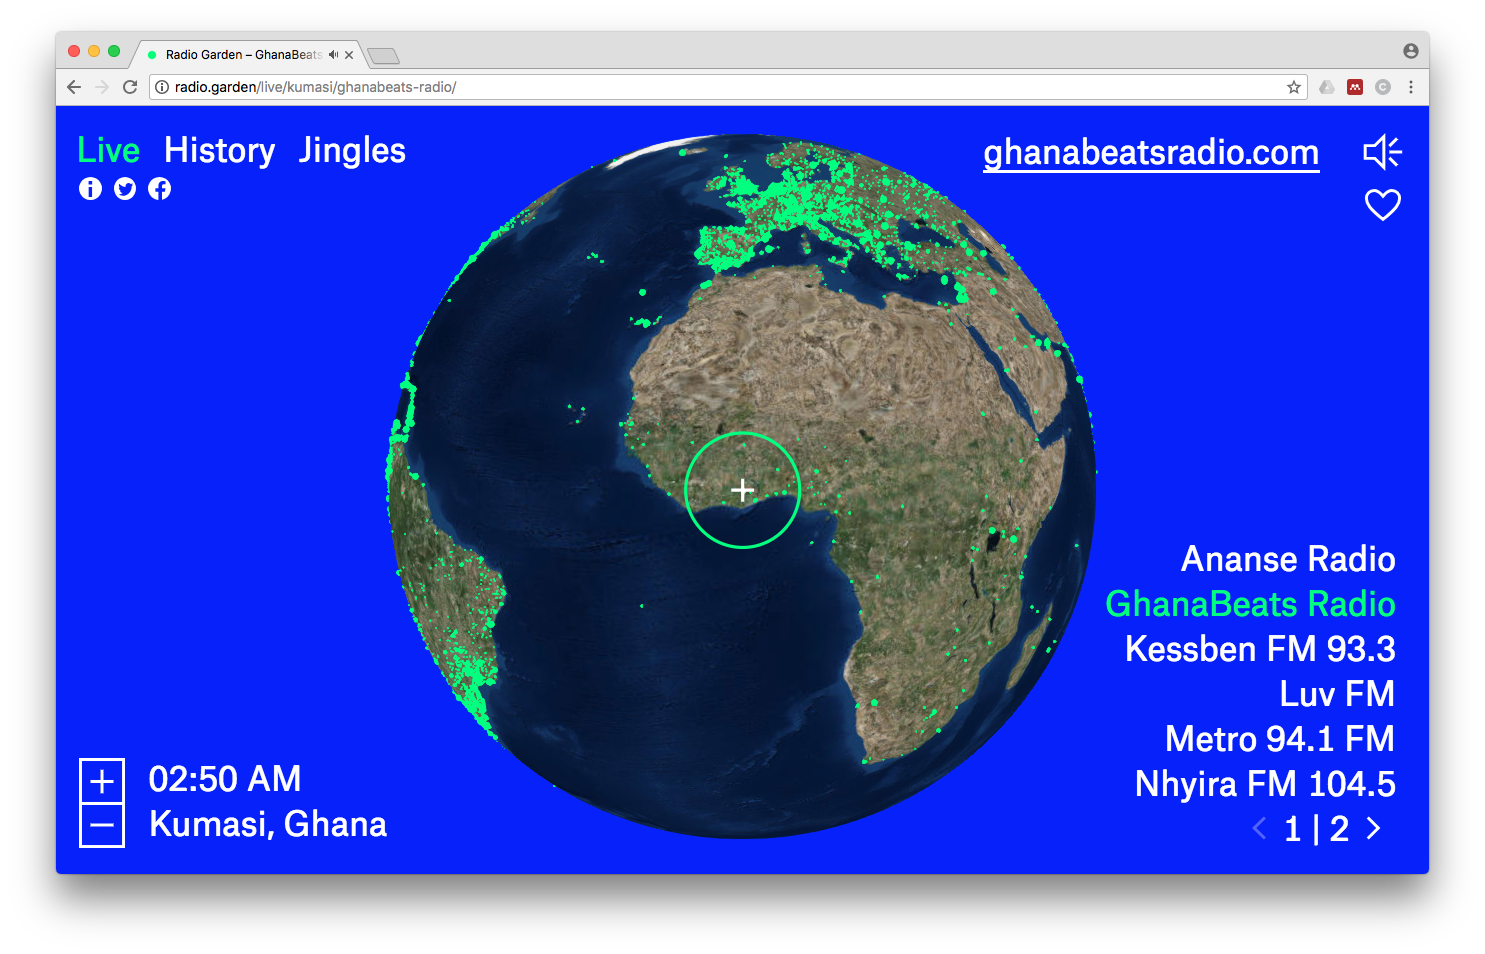
\includegraphics[width=1\linewidth]{pictures/radio_garden_2018-06-10.png}
    \end{center}
    \legend{Fonte: Screenshot da autora, 8 de junho de 2018}
    
\end{figure}
%\legend{Fonte: \citeonline[p. 24]{araujo2012}}

Posso também acessar uma base de dados extensiva da produção humana em música, cinema e televisão construída a partir do trabalho de pessoas em todo o planeta, reunida em grandes portais como o Youtube, onde segundo estatísticas atuais são depositadas 300 horas de conteúdo a cada minuto, mas, como bem apontou a compositora Pauline Oliveros em ``Software for people", ``As mídias e a maior mobilidade obviamente acomodam mais informação, mas não necessariamente mais sabedoria"\cite[179]{Oliveros2012}. 

Os teóricos da sociedade da informação professavam que a internet teria um papel demiúrgico, que ``libertaria a humanidade sem qualquer necessidade de luta de classes" \cite[275]{Barbrook2009}, mas sob a neoliberal "ideologia californiana", a internet se transformou na apoteose do mercado (idem, p. 353). Há quem inclusive culpe a mídia eletrônica por exacerbar uma série de de males da sociedade como: "elitismo, pedofilia, terrorismo, deficiência educacional e solidão" (idem, p. 59). 

\todo[inline]{fake news}

Não é difícil de concordar com essa visão. Uma simples tecnologia que permite ao usuário deixar sua opinião nas notícias dos grandes portais é suficiente para nos assombrar com o nível de barbárie latente na sociedade, a cada notícia veiculada na supostamente isenta ``grande mídia". Abre espaço para a voz do Zé Ninguém, como definido por Wilhem Reich \cite{reich1998escute}, aquele ser de mentalidade tacanha, que "está sempre do lado dos perseguidores" (p. 27), que persegue mães solteiras, por serem imorais, ao mesmo tempo que cultua Jesus, que ``é tolerante com a sua própria religião mas com nenhuma outra (p.51)":

\begin{citacao}
como não tem memória para coisas que aconteceram há dez ou vinte anos, você ainda repete os mesmos disparates de dois mil anos atrás. Pior, você se agarra com unhas e dentes a absurdos como "raça", "classe", "nação" e à obrigação de seguir uma religião e reprimir sua desgraça. \cite[101]{reich1998escute} 
\end{citacao}

Apesar disso, nós, que somos artistas, pesquisadores e pessoas que criam, não podemos nos sujeitar passivamente à essa visão apocalíptica de que a internet está nos levando à barbárie, e podemos pensar nos meios tecnológicos como ponto de partida para novas proposições éticas e estéticas. Concordamos com arquiteto e pintor Sérgio Ferro quando afirma: que a expressão humana na arte é ``pegar a necessidade histórica que está no material e trabalhá-la até o fundo", \cite{FerroSergio2002} e que isto é a própria essência da liberdade.

 \todo[inline]{programação como potencia}

A música, dentre as demais formas de arte é muito potente, no sentido de que o som é quase impossível de se bloquear. Ela tem a capacidade de atingir as pessoas circundantes de uma maneira geral e compulsória, a energia sonora é das mais difíceis de se conter em termos coletivos. É possível um indivíduo tampar seus próprios ouvidos, mas é muito difícil tapar os ouvidos alheios, e mesmo tampando os ouvidos, nunca haverá silêncio. Levinson (1999) aponta que o som tem como característica "emanar de todos ambientes", e enquanto a visão nos dá detalhes preciso, ponto-a-ponto do ambiente ao nosso redor, é a audição que ``nos mantém em contato com o mundo vinte e quatro horas por dia" \cite[47]{Levinson2001}. 

\todo[inline]{Acredito que esse poder pode ser uma das razões pela qual a sociedade patriarcal tende a manter as mulheres longe dos instrumentos musicais.}  

Minha relação com a produção musical teve muita relação com esse potencial de agregação que a música traz, primeiro, como dj, organizando festas que eram essenciais para o financiamento do grêmio dos estudantes da FAU, depois, no Urbando, grupo de maracatu que intervinha também em atos estudantis, e sempre foi muito nítido pra mim o potencial de um tambor ou um xequerê como instrumento de organização de massas em atos, como instrumentos para colocar as pessoas em movimento. Não é atoa que os exércitos usam marchas como forma de elevar a moral dos soldados, e que também as igrejas usem música para encantar os fiéis. O discurso verbal pode ser cansativo, o texto pode ser ignorado, enquanto a música é capaz de colocar uma multidão em uníssono. Em uma sociedade como a nossa, esse poder é exercido principalmente pela indústria cultural, que afasta esse sentido político que a música pode ter, convertendo tudo em mercadoria, como aponta Marilena Chauí no seu artigo "Cultura e Democracia": 

\begin{citacao}

Como cultura de massa, as obras de pensamento e de arte tendem: de expressivas, tornarem-se reprodutivas e repetitivas; de trabalho da criação, tornarem-se eventos para consumo; de experimentação do novo, tornarem-se consagração do consagrado pela moda e pelo consumo; de duradouras, tornarem-se parte do mercado da moda, passageiro, efêmero, sem passado e sem futuro; de formas de conhecimento que desvendam a realidade e instituem relações com o verdadeiro, tornarem-se dissimulação, ilusão falsificadora, publicidade e propaganda. mais do que isso. A chamada cultura de massa se apropria das obras culturais para consumi-las, devorá-las, destruí-las, nulificá-las em simulacros. Justamente porque o espetáculo se torna simulacro e o simulacro se põe como entretenimento, os meios de comunicação de massa transformam tudo em entretenimento (guerras, genocídios, greves, festas, cerimônias religiosas, tragédias, políticas, catástrofes naturais e das cidades, obras de arte, obras de pensamento). É isto o mercado cultural. \cite[61]{MarilenaChaui2008}
\end{citacao}

Uma cultura democrática, seria aquela, segundo ela, onde as pessoas tenham acesso aos meios de produção cultural, e não somente aos produtos de seu mercado. Tendo uma formação em arquitetura e design, e sendo assim de certo modo estranha ao contexto e aos códigos da música tradicional, foi fácil notar o alto grau de fechamento da cena musical, especialmente para mulheres, como aponta Pauline Oliveros no texto ``And don't call them Lady Composers" \cite[48]{Oliveros2012}. Uma das coisas que colabora com esse hermetismo é a dificuldade de acesso aos instrumentos musicais, que podem ser muito caros, pesados ou de difícil manipulação. 

\todo[inline]{Parti minha pesquisa então dessa questão do acesso, uma vez que sendo mulher, pequena e trabalhadora, é uma questão fundamental na minha prática artística cotidiana.}


O acesso aos meios de produção certamente é uma das barreiras que afasta as pessoas de uma vivência musical cotidiana. Instrumentos musicais, equipamentos de áudio em geral e controladores, podem ser muito caros, complexos e de difícil manipulação\cite{Fiebrink2007} . "Ubiquitous music research is not just yet
another approach to musical interaction. It is a new way to foster music making in contexts
that were previously not accessible to artistic endeavors." \cite{Keller2018}

A digitalização das tecnologias de produção musical, no entanto, tornou acessível aos usuários de computadores pessoais, tecnologias que só eram disponíveis para grandes estúdios musicais. A partir dos anos 80, isso causou um crescimento exponencial do engajamento da juventude com meios de produção musical digitais, como aponta Georgina Born \cite[143]{Born2015}, mas também causa a uma "tecnofilia fetichista" em relação a equipamentos e tecnologias (idem, p. 145).

Como aponta Baudrillard em ``O sistema de objetos", ``os consumidores não têm acesso à igualdade diante do objeto depois da Revolução Industrial" \cite[162]{Baudrillard2012}. Podemos dizer que a revolução digital, tem permitido concentrar uma série de funcionalidades em gadgets como celulares ou laptops, cada vez menores e mais complexos, que exercem cada vez mais uma dominação dos sentidos individuais das pessoas – que ficam dependentes e absortas em complexas tramas de dados e dramas. O gadget para Baudrillard é um objeto que faz parte de um universo de delírio funcional, um tecnicismo excêntrico e formalismo gratuito, objetos tomados totalmente pelo imaginário, ou obsessões pura e simples, aberrações funcionais. (idem p.121). 

Meu projeto parte de um desejo de libertação dessa dependência de toda uma uma parafernália tecnológica, concentrando esforços em desenvolver protótipos experimentais para produção musical em tecnologias para a rede. Soluções deste tipo podem ser mais acessíveis, já que um instrumento musical online poderia ser acessado por qualquer dispositivo que tenha acesso à internet -- como computadores ou smartphones -- gadgets que ganharam muito poder de processamento, nos quais já estamos absortos. Além disso, tinha um desejo sobretudo de investigar novas formas de interface, por considerar que muitas das interfaces existentes, que são em maioria baseadas nas de equipamentos eletrônicos \cite{Stolfi2016}, também exigem a necessidade de saberes bastante específicos em tecnologias musicais, além de imporem certos parâmetros da música tradicional, como notas, timbres e tempos. 

Com o desenvolvimento da pesquisa, e o meu contínuo envolvimento com práticas musicais como a da improvisação livre, ``uma pragmática musical aberta à variação infinita em que os sistemas e as linguagens deixam de impor suas gramáticas abstratas e se renderem a um fazer fecundo" \cite[2]{Costa2016} esse desejo de construção de instrumentos genéricos foi se direcionando para a construção de instrumentos específicos para suprir necessidades pessoais musicais -- como é o caso do projeto Banda Aberta e o Playsound, projetos que descreverei mais a frente nesta tese -- sempre buscando portabilidade e facilidade de uso.


\subsection{interfaces não gesturais}

Na música tradicional, o gesto -- do performer ou do intérprete -- é tradicionalmente o gerador do som. O domínio do ato de tocar, principalmente instrumentos tradicionais, envolve um domínio de uma linguagem corporal que gera o som desejado de acordo com o desejo do musicista. Na música instrumental e vocal, sempre há um gesto físico que gera o som, o que não acontece necessariamente na música eletrônica \cite[85]{Smalley1996}. Isto é uma preocupação de quem desenvolve aplicativos para música interativa, como aponta Schnell (2013). 


\begin{citacao}
Two principal concerns constitute the design of interactive audio applications and musical in- struments of virtually any kind. One deals with creating real-time interactive sound processes and the other with the way these sound processes are influenced by the bodily movements and gestures of their players. In this sense, the essence of designing interactive audio applications lies in the creation of meaningful relationships between movement – or gestures – and sound. \cite{Schnell2013}
\end{citacao}
Essa questão já é discutida no âmbito das laptop orchestras, como aponta Trueman (2007):
\begin{citacao}
For the laptop performer, this seems to pose a
deep problem. If we look like we are simply doing e- mail while generating sounds that provoke the motor-mimetic response of, say, striking an enormous hammer, what will the ‘listener’ make of it all? What kind of vicarious performance could this possibly inspire?What would the ‘air-laptop’ dance look like? 
But perhaps this is an opportunity instead of a problem, a challenge for which the laptop orchestra is a musically and socially charged gymnasium. On the one hand, we can go at it head-on and endeavour to create challenging instruments that generate sounds which somehow seem tangibly (even acoustically) related to the physicality they demand.





\cite[6]{Trueman2007}
\end{citacao}

\subsection{agência}


A noção de virtuosidade, para Smalley (1996) é baseada na identificação de um controle consumado na articulação de morfologias sonoras. No seu modelo do espectro de sons, Smalley considera como sons musicais, aqueles gerados com intenção pelos homens, mesmo sons naturais, podem ser convertidos em música desde que sejam resultado de uma agência humana. O campo da música eletroacústica foi responsável por inserir na música uma ampla gama de sons sintetizados e da natureza que não necessariamente podem nem ter tido uma existência material. Muitos trabalhos acusmáticos, inclusive, não possuem nenhuma fonte sonora gestual visível em tempo real \cite[95, 101]{Smalley1996}.



\todo[inline]{Para estruturar essa pesquisa em uma tese de doutorado, partirei de uma conceituação teórica a respeito de alguns temas que norteiam essa pesquisa: 
o princípio da antropofagia, que envolve procedimentos práticos e teóricos da nossa metodologia; 
a idéia de interdisciplinaridade como prática, e relações estabelecidas entre design, música e tecnologia; 
a idéia de cultura livre, defendida por uma série de ativistas da cultura digital; 
a estética do brutalismo digital verbivocovisual e suas referências históricas; 
a noção de música prática e experimental como espaço de liberdade.
Em seguida, vou reunir alguns recursos utilizados durante esta pesquisa, de modo a fornecer uma base de conhecimentos para quem se interesse por práticas semelhantes. Tratarei de recursos como servidores de internet, ferramentas e linguagens úteis até e recursos para produção de performance e apresentações tentado buscar um set-list mínimo de equipamentos e cabos. 
O capítulo seguinte, tratará do processo de pesquisa em si, partindo de primeiras experiências de pesquisa em redes e em interfaces para produção e difusão musical, como a música me levou à internet e como a internet me levou à música, através de práticas junto a coletivos, grupos de discussão e práticas artísticas em grupo, até os experimentos desenvolvidos junto ao grupo de pesquisa NuSom, na Universidade de São Paulo, como o projeto Banda Aberta, o Spectrogram player e outras experiências em música interativa que estou desenvolvendo. 
Por fim, apresentarei nas considerações finais, algumas questões éticas e estéticas levantadas  ao longo da pesquisa, conclusões e resultados dos experimentos aqui desenvolvidos, bem como limitações e potencialidades para desenvolvimentos futuros.
}


\subsection{Cultura Livre}

Procuramos defender uma idéia de cultura livre, que permeia uma série de práticas, desde a escolha das linguagens, do repertório e dos projetos, até a publicação de código aberto e conteúdo em licenças livres. A própria adoção de práticas de improvisação livre tem relação com essa idéia. A digitalização da arte leva à possibilidade de livre reprodução, e amplia sua sua exponibilidade, como já apontava Benjamin (1987). A própria web foi construída com base em idéia de livre circulação da informação, na adoção de uma estrutura não hierárquica e de linguagens livres de marcação (Berners-lee, 1989).
A cultura livre é defendida por uma comunidade de pensadores, programadores e artistas, como Lawrence Lessig (2004), e a iniciativa Creative Commons, Richard Stallman e a comunidade do software livre, e mesmo Alexandra Elbakyan com o Scihub que desafia constantemente a propriedade da informação, (Barok et al, 2015) entre vários outros que têm constantemente militado por diversas práticas culturais libertárias.



\subsection{Brutalismo Digital}
Neste subtema, procurarei falar de referências estéticas, e especialmente da influência da arquitetura moderna e do brutalismo de Vilanova Artigas e da precariedade radical de Lina Bo Bardi, dos concretistas russos como El Lissitsky e Rodchenko e brasileiros como Sacilotto, Athos Bulcão e Lygia Pape, Erthos Albino de Souza, Augusto de Campos, Haroldo de Campos e Décio Pignatari. Trabalhar a partir de  referências do passado pode trazer certas questões ideológicas, como aponta Plaza (idem, p. 6):
Operar sobre o passado encerra um problema de valor. Não é escolher um dado do passado, uma referência passada; é uma referência a uma situação passada de forma que seja capaz de resolver um problema presente e tenha afinidade com suas necessidades precisas e concretas, de modo a projetar o presente sobre o futuro. Toda época distingue entre formas conservadoras e mais inovadoras. As inovadoras são as que se projetam para o futuro através do caráter inacabado que aponta para um possível leitor, o que é também uma forma de ``perceber na cultura de hoje os traços reais e inconfundíveis do amanhã''. Operar sobre o passado, além de um problema de valor, constitui-se também numa operação ideológica através da qual podemos confirmar a produção do presente ou encobrir essa realidade. Se, no primeiro caso se favorece um encontro dialético com o passado para preparar o futuro, no segundo, trata-se de distanciar esse futuro indefinidamente. No primeiro caso, os valores da história constituem-se num modelo para a ação, já no segundo, trata-se de um fantasma a ser evocado como nostalgia, moda ou revival.
Aqui, não queremos trazer essas referências como inspiração ou nostalgia, mas como apontamentos para pensar possibilidades estéticas. Como os princípios de racionalidade,  e sobretudo uma postura anti-decorativa, anti-ornamental e de procurar um mínimo de elementos necessários. 

\subsection{Trans-disciplinaridade}
No artigo "Logics of interdisciplinarity", Barry, Born e Weszalnys apontam o campo interdisciplinar da Arte-ciência, como um campo emergente, onde "a prática corre na frente da teoria" (BARRY, A.; BORN, G.; WESZKALNYS, G, 2008, p. 38), que pode ter como um dos objetivos "desafiar e transformar formas existentes de pensar sobre a natureza da arte e da ciência, bem como as relações entre artistas e cientistas e seus objetos e públicos" , segundo eles, invenção e originalidade na arte-ciência se sustentam melhor nas práticas onde os artistas conseguem fazer uso de laboratórios, oficinas e computadores (idem, p. 39). Isto é reforçado se observarmos os trabalhos de alguns pioneiros da arte digital, como Erthos Albino de Souza, Waldemar Cordeiro, Nam Jum Paik e Júlio Plaza. 
Plaza aponta que intermídia e multimídia são "categorias interdisciplinares  que colocam em questão as formas de produção-criação individual"  (Plaza, 2013 p. 66) e que as formas eletrônicas tem um caráter abrangente que dialoga "intersensorialmente" com vários códigos da informação, "uma hibridização de meios, códigos e linguagens que justapõem e se combinam" (idem, p. 13)

\subsection{Antropofagia}

    % Write epigraphs
    \begin{flushright}
        \textit{``A síntese
O equilíbrio
O acabamento de carrosserie
A invenção
A surpresa
Uma nova perspectiva
Uma nova escala
Qualquer esforço natural nesse sentido será bom.''} \\
Oswald de Andrade – Manifesto Pau Brasil    \end{flushright}

``A alegria é a prova dos nove'', aponta Oswald no Manifesto Antropófago. Desde meus primeiros envolvimentos com música e performance no Coro de Carcarás, por volta de 2005, a influência da antropofagia Oswaldiana foi bastante significativa. Neste capítulo procurarei tratar especificamente desta influência, bem como da de artistas que tomaram esse princípio para suas práticas, como Lygia Clark e Hélio Oiticica, neste que tem um certo aspecto de devoração do outro e um sentido de busca de alegria e liberdade, relacionando também com práticas correntes junto a redes como a do tecnoxamanismo, que trouxeram novas perspectivas neste sentido.

\subsection{Música Prática}

\begin{citacao}


The hardest thing for a digital musician to decide is not what skills should be acquired but what not to learn. Given that the skill set draws upon so many different and well- established disciplines, it is always possible to go further into any one of them in order to specialise in a particular area. A theme that emerges, there- fore, is the sheer number and variety of employment situations or careers. Here is a quick list of just some of them: programmer, music and effects for games, music and effects for cinema (location sound, ADR, Foley, sound effects, re-recording engineer, composer, session engineer, etc.), music and effects for industrial video, audio- loops designer, audio- effects designer, mobilephone ringtone designer, radio producer, studio engineer, record producer, mastering engineer, music- related retail sales, music software support, jingle writing, music- events producer, live- sound engineer, band member, session musician, arts administrator, self- promoted musician, Internet- based microsales, record- label manager, talent scout, A\&R (artist and repertoire) representative, acoustic designer, arts/sound museum\/events coordinator, events\/festivals technical support, PA system con- sulting and installation, DSP inventor, instrument inventor, writer for electronic music magazines, sound for web (commercial record sales samples, sound design for sites, interactive sound), bulk media reproduction, teaching, music therapy, new- age market (relaxation tapes, mind manipulation, etc.), Muzak, corporate sonic environments, multimedia development, busking, lawyer, music librarian, artist.\cite[191]{Hugill2012}
\end{citacao}


gravação, edição e sequenciamento
processamento de sinais (incluindo plugins)
samplers
instrumentos virtuais (vst)
sintetizadores
performance ao vivo
notação
composição
análise e representação
modulares ou construíveis

\begin{citacao}
Music production relies on software. To specify precisely which music software packages might be useful to the musician is futile, because the software market changes so rapidly. However, it is possible to identify generic types of music soft- ware, as follows:
• sound recording, editing and sequencing software • processing applications (including plug- ins) • software samplers • virtual instruments • synthesis software • live- performance software • notation software • composition software • analysis or representation software • modular or build- it- yourself software.\cite[195]{Hugill2012}
Additions
\end{citacao}


The digital musician will need to be aware that such software can try to steer musical content in a particular direction, even towards a specifi c genre or style. Sometimes music production is a matter of fi nding ways to achieve some- thing original in spite of the software design. \cite[195]{Hugill2012}


\begin{citacao}
A nosso ver, se devemos operar \emph{em} e \emph{para} um mundo construído na medida humana, essa medida será individuada não adaptando o homem a essas condições de fato mas \emph{a partir dessas condições de fato}. O universo das comunicações de massa é -- reconheçamo-lo ou não -- o nosso universo; e se quisermos falar de valores, as condiçnoes objetivas das comunicações são aquelas fornecidas pela existência dos jornais, do rádio, da televisão, da música reproduzida e reproduzível, das novas formas de comunicação visiva e auditiva. Ninguém foge a essas condições, nem mesmo o virtuoso, que, indignado com a natureza inumana desse universo da informação, transmite o próprio protesto através dos canais de comunicação em massa, pelas colunas do grande diário, ou nas páginas do volume em \emph{paperback}, impresso em linotipo e difundido nos quiosques das estações.\cite[13]{Eco1970}


\end{citacao}

estamos em plena indústria cultural, e um operador de cultura, deve segundo Eco
\begin{citacao}
Colocar se em relação dialética, ativa e consicente com os condicionamentos da indústria cultural tornou-se para o operador de cultura o único caminho para cumprir sua função. \cite[14]{Eco1970}
\end{citacao}


    \newpage

     \emph{}

    \section*[Some encoding tests]{Some encoding tests}

    % Why latex is letting my text goes out of the screen?
    % https://tex.stackexchange.com/questions/386762/why-latex-is-letting-my-text-goes-out-of-the-screen
    \sloppy
    \textbf{textbf:  }
    \fussy

\end{otherlanguage*}




A Tabela~\ref{tab:a_table_formatacao_de_texto} mostra mais informações do template BU.

% What does [t] and [ht] mean?
% https://tex.stackexchange.com/questions/8652/what-does-t-and-ht-mean
%
% How can I get rid of the LaTeX warning: Float too large for page?
% https://tex.stackexchange.com/questions/36252/how-can-i-get-rid-of-the-latex-warning-float-too-large-for-page
%
% "warning: Text page X contains only floats" How to suppress this warning?
% https://tex.stackexchange.com/questions/223149/warning-text-page-x-contains-only-floats-how-to-suppress-this-warning
%
% Make a table span multiple pages
% https://tex.stackexchange.com/questions/26462/make-a-table-span-multiple-pages
%
% How to make the longtable to work with centering & caption on memoir class?
% https://tex.stackexchange.com/questions/386541/how-to-make-the-longtable-to-work-with-centering-caption-on-memoir-class
%
% How to fix this Package array Error: Only one column-spec allowed?
% https://tex.stackexchange.com/questions/367069/how-to-fix-this-package-array-error-only-one-column-spec-allowed
%
% How to auto adjust my last table column width, and why is there Underfull \vbox badness on this table?
% https://tex.stackexchange.com/questions/387238/how-to-auto-adjust-my-last-table-column-width-and-why-is-there-underfull-vbox/387251
\setlength\extrarowheight{2pt}
\begin{tabularx}{\linewidth}{>{\RaggedRight}p{3cm}|>{\arraybackslash}X}

\caption{Formatação do texto \protect }
\label{tab:a_table_formatacao_de_texto} \\
\hline
\endfirsthead

% How to set font size of footnotes correctly in memoir?
% https://tex.stackexchange.com/questions/213927/how-to-set-font-size-of-footnotes-correctly-in-memoir
\multicolumn{2}{p{\dimexpr\textwidth-2\tabcolsep\relax}}{\ufsccaptionsize\tablename~\thetable:
Formatação do texto (continuação) \protect } \\
\hline
\endhead

% Set multicolumn width to default table width
% https://tex.stackexchange.com/questions/99326/set-multicolumn-width-to-default-table-width
\hline
\multicolumn{2}{p{\dimexpr\textwidth-2\tabcolsep\relax}}{\footnotesize continua na próxima página\protect }
\endfoot

\hline
\endlastfoot

    Cor                          & Branco -                                                 \\ \hline
    Formato do papel             & A5                                                               \\ \hline
    Gramatura                    & 75                                                               \\ \hline
    Impressão                    & Frente e verso                                                   \\ \hline
    Margens                      & Espelhadas: superior 2, Inferior: 1,5, Externa 1,5 e Externa: 2. \\ \hline
    Cabeçalho                    & 0,7                                                              \\ \hline
    Rodapé                       & 0,7                                                              \\ \hline
    Paginação                    & Externa                                                          \\ \hline
    Alinhamento vertical         & Superior                                                         \\ \hline
    Alinhamento do texto         & Justificado                                                      \\ \hline
    Fonte sugerida               & Times New Roman                                                  \\ \hline
    Tamanho da fonte             & 10,5 para o texto incluindo os títulos das seções e subseções.
                                   As citações com mais de três linhas as legendas das ilustrações
                                   e tabelas, fonte 9,5.                                            \\ \hline
    Espaçamento entre linhas     & Um (1) simples                                                   \\ \hline
    Espaçamento entre parágrafos & Anterior 0,0; Posterior 0,0                                      \\ \hline
    Numeração da seção           & As seções  primárias devem  começar  sempre em páginas ímpares.
                                   Deixar um espaço (simples) entre o título da seção e o texto e
                                   entre o texto e o título da subseção.                            \\ \hline

\end{tabularx}













    % PARTE
    % \ifforcedinclude\else\part{Preparação da pesquisa}\fi

    % Capitulo com exemplos de comandos inseridos de arquivo externo
    % The \phantomsection command is needed to create a link to a place in the document that is not a
% figure, equation, table, section, subsection, chapter, etc.
%
% When do I need to invoke \phantomsection?
% https://tex.stackexchange.com/questions/44088/when-do-i-need-to-invoke-phantomsection
\phantomsection


% Multiple-language document - babel - selectlanguage vs begin/end{otherlanguage}
% https://tex.stackexchange.com/questions/36526/multiple-language-document-babel-selectlanguage-vs-begin-endotherlanguage
\begin{otherlanguage*}{brazil}

    \chapter
    [Percurso]
    {Perscurso}


    \begin{flushright}
     
    \end{flushright}


    % \newpage

\linespread{1.5}

    \section{A música me levou à rede}
    
    Meus primeiros contatos com a World Wide Web foram em 1996, na época, tínhamos que ir até uma das salas em um laboratório da Poli, usar a rede em uns computadores Sun, já que não havia ainda servidores acessíveis em casa. Lembro, que minha atividade preferida na época era a coleta de letras de música, que eu imprimia e levava para a escola para cantarmos nos intervalos. Para ouvir música, no entanto, haviam as rádios, a MTV, uns poucos discos e CDs comprados ao longo dos anos e as fitinhas gravadas do rádio. O repertório acessível era muito reduzido, embora uma inclinação familiar para música "séria" garantiu um certo contato com um repertório tradicional da música contemporânea, jazz e música popular brasileira. Em casa, usava os computadores principalmente para jogar.


\todo[inline]{desenvolver sobre pirataria}
    \begin{citacao}
Comparados aos seus antecessores, as ambições dessa subcultura jovem aparentemente apolítica pareciam muito mais modestas: compartilhar músicas bacanas pela Internet. Entretanto, para a indústria da música, essa utopia hacker era um negócio desastroso. Pregar a revolução, tomar drogas e a perversão sexual eram práticas que podiam ser toleradas dentro desse empreendimento capitalista descolado. Tudo era permitido no maravilhoso mundo pop, com somente uma exceção: a música livre.\cite[370]{Barbrook2009}
\end{citacao}

Quando surgiu o Audiogalaxy, que inaugurou a era dos softwares peer-to-peer, é que para mim ter internet realmente começou a fazer sentido. Na tela azul do site, um mapa de possibilidades que iam surgindo a cada download; o site oferecia um sistema de de sugestões, que mostrava outros artistas que ouvintes de uma determinada canção gostavam. Nesse período, consegui ter uma ampliação gigante do repertório, passando de uma centena de cds para milhares, descobrindo coisas tão diversas como as primeiras gravações de blues americanas, as várias nuances de música eletrônica do começo dos anos 2000 e a música popular brasileira. 



Com essa pesquisa de repertório adquirido na internet, através da nova cultura de dádiva que se estabelecia, acabei assumindo a posição de DJ em alguns happy hours quando em 2001 participei pela primeira vez da gestão do Gfau, o grêmio de estudantes da FAU, junto à chapa "Estúdio 5". Foi nesse ano também que comecei a desenvolver um interesse especial pelo design de interfaces, fazendo algumas experiências com animações em flash, entre elas o site para a Expofau 2001, que aconteceu naquele ano com cerca de 150 trabalhos inscritos. Mas ainda era para a mídia impressa que eu dedicava mais atenção e força de trabalho. Fiz uma iniciação científica bem técnica em design gráfico, investigando legibilidade de texto e me engajei em diversas comissões do Gfau, grupos de extensão e organizações estudantis dos quais fiz parte – Revista Caramelo, Jornal 1:100, Labhab gfau, Grupo Anita Garibaldi, Revista Contravento e da fundação da Negação da Negação – pude experimentar com várias técnicas de composição gráfica digitais e analógicas. Foi uma época de extensa produção estudantil, do surgimento da "Fau Paralela", "expressão dessa consciência de que a escola e o aprendizado estão em grande parte fora da instituição, do curricular", como aponta Ana Carolina Ribeiro (2006) no seu TTG "trans Forma Ação, que analisa a produção gráfica da FAU na época. 

Nessa época, comecei a desenvolver as primeiras pesquisas em composição gráfica modular, que chamava de "Concretismo Tosco", pela inspiração concreta e a precariedade no acabamento, uma influência do pensamento do arquiteto Sérgio Ferro, que defendia a manutenção do erro como um marca do trabalho na obra de arte (Ferro, 2001). 

Em 2005, o professor belga Etienne Delacroix veio ao Brasil oferecer a disciplina "Oficina de Arte e Programação" na Poli, que tive oportunidade de cursar como optativa. Ele instalou numa sala o Atellier Labs, uma mistura de laboratório e atelier, onde os alunos poderiam desenvolver projetos de seu interesse, relacionados com os temas que o professor nos apresentava, que iam de reciclagem de computadores, instrumentos musicais DIY, robôs, software livre e programação para web. O Atellier Labs foi um verdadeiro centro difusor de cultura livre em São Paulo, tendo colaborado com a formação de uma rede de ativistas em cultura digital que atuam até hoje em diversas cidades do Brasil. 

Em 2005, o professor belga Etienne Delacroix veio ao Brasil oferecer a disciplina "Oficina de Arte e Programação" na Poli, que tive oportunidade de cursar como optativa. Ele instalou numa sala o Atellier Labs, uma mistura de laboratório e atelier, onde os alunos poderiam desenvolver projetos de seu interesse, relacionados com os temas que o professor nos apresentava, que iam de reciclagem de computadores, instrumentos musicais DIY, robôs, software livre e programação para web. O Atellier Labs foi um verdadeiro centro difusor de cultura livre em São Paulo, tendo colaborado com a formação de uma rede de ativistas em cultura digital que atuam até hoje em diversas cidades do Brasil. 

\section{A rede me levou à música}
O envolvimento nas atividades políticas estudantis, levou à participação em uma série de atividades musicais, inicialmente com a organização de festas, depois como percussionista no grupo Urbando, um núcleo do Gfau que atuava em festas e manifestações estudantis e posteriormente em atividades de livre improvisação que aconteciam às quintas feiras no gramado da FAU, o Som de Quinta. Esse engajamento me levou a uma paixão pela música como atividade prática e cotidiana, não mais somente como ouvinte. 
Comecei também a produzir música eletrônica, em um software que se chamava Jeskola Buzz, um software gratuito meio obscuro, que era usado por alguns artistas da cena eletrônica, funcionava uma plataforma aberta – embora não open-source – para a criação de instrumentos, chamadas machines, e oferecia uma ampla gama de sintetizadores e efeitos de áudio. O Buzz tinha uma interface bastante peculiar, que alternava três espaços:

um para estabelecer rotas de comunicação entre de processamentos de sinais digitais (DSP) (figura x);
um para desenhar padrões para os instrumentos e efeitos, que lembrava um cartão perfurado. Os parâmetros eram definidos em linguagem Hexadecimal e as notas no sistema de notação americano (Ex: C-3, etc) (figura x);
uma linha do tempo, onde se podia distribuir os padrões desenhado ao longo do tempo;

Com ele, pude desenvolver uma série de conhecimentos práticos em métodos de síntese e processamento de áudio, que organizei em experimentos sonoros metalinguísticos, chamados de Protomúsica. Metalinguísticos porque o próprio processo de composição levava em conta uma experimentação com os instrumentos e os materiais musicais, por exemplo:
Em estudo de harmonia e dissonância num ré. Disponível em: \url{http://finetanks.com/records/2005_2010/protomusica/estudo\%20de\%20harmonia\%20e\%20dissonancia\%20num\%20re.mp3} >, procurei explorar as possibilidades de intervalos musicais em um sintetizador aditivo;
Em Dodecafunk, procurei fazer uma batida funk com uma melodia que seguisse regras dodecafônicas. Disponível em: \url{http://finetanks.com/records/2005_2010/protomusica/dodecafunk.mp3}
Em percussiva, explorei as possibilidades de variação de timbre a partir de um padrão rítmico de apenas uma nota no sintetizador percussive FM. Disponível em: \url{http://finetanks.com/records/2005_2010/protomusica/percussiva.mp3}

Com o provedor, comecei a organizar um site para colocar materiais de produções minhas, e convidei alguns colegas que produziam também para publicar online no site Finetanks.com, que tinha também algumas ilustrações de Guilherme Garbato, minha pesquisa de iniciação científica, "Legibilidade e Evolução das Mídias, desenvolvida entre 2000 e 2001, e alguns primeiros experimentos em arte interativa; uns painéis modulares randômicos programados em php, inspirados nas obras de Athos Bulcão.  
Os primeiros projetos hospedados no Finetanks foram duas bandas punks, Os Otávios e Desprezíveis, de amigos do movimento estudantil, o Cabeça de Câncer, projeto de improvisação com Guilherme Garbato e Fernando Bizarri e o meu projeto solo de música eletrônica, Protomúsica. Com o tempo, foram anexados outros projetos como o JazzMetak e Freetools, de free jazz e Organograma, projeto de música eletrônica de Fernando Bizarri.

\subsection{Cultura Digital}

Depois logo após a graduação, comecei a trabalhar como pesquisadora na equipe do Hacklab, um grupo de desenvolvedores web que atuava em São paulo financiados pelo projeto Cultura Digital, do Ministério da Cultura (MinC), para fornecer recursos para os pontos de cultura, que chegavam a 1000 unidades em 2006 (LIMA e SANTINI, 2009, p. 5). Os pontos de cultura foram criados em 2004 na gestão de Gilberto Gil do MinC, para fomentar espaços culturais independentes em todas as regiões do país, ou segundo ele próprio Gil:
\begin{citacao}

``Para fazer uma espécie de do-in antropológico, massageando pontos vitais, mas momentaneamente desprezados ou adormecidos, do corpo cultural do País. Enfim, para avivar o velho e atiçar o novo. (Gil 2003)" 
\end{citacao}


Entre os projetos que estavam sendo desenvolvidos pela equipe do hacklab estava o \url{Estudiolivre.org}, que tinha como objetivo "a formação de espaços reais e virtuais que estimulem e permitam a produção, a distribuição e o desenvolvimento de meios de comunicação e de informação livres" (idem, p. 12) e oferecia ferramentas para download e compartilhamento de arquivos de imagem, som e vídeo, além de manuals, fóruns e páginas pessoais, e é considerado um projeto pioneiro na cultural digital no Brasil. 

O trabalho no Hacklab me colocou em contato com grupos diferentes de pessoas atuantes nos circuitos de produção de cultura livre, em diferentes redes, como a Merareciclagem, Estudiolivre, Coletivo Coro, CMI e a Rede Saravá. Foi também uma época de intensa produção musical amadora, de marchinhas carnavalescas e músicas pop, muitas das quais não foram gravadas. 

\todo[inline]{cultura livre/pontos de cultura e cultura digital}

\subsection{Records}
Em 2010, comprei um gravador estéreo portátil e comecei a fazer algumas gravações em campo. Durante os festivais Submidialogias, em Arraial D'Ajuda e em Paranaguá e o Ruidocracia no Rio de Janeiro, gravei uma série de encontros musicais, jams e processos um tanto catárticos de improvisação e composição coletiva, em conjunto com Felipe Ribeiro, Jerônimo Barbosa, Fabiane Borges, Ricardo Brasileiro, Glerm Soares, Kaloan Menochite, entre outros. Passei então a editar o material gravado e transformei o Finetanks em uma pequena gravadora independente. Não havia suporte para áudio ainda na linguagem HTML, e para construir as páginas dos projetos era preciso inserir iframes com o endereço dos arquivos originais, processo que era relativamente trabalhoso e bastante artesanal, então, em 2010 o site foi transformado em um repositório, sem páginas em HTML para cada projeto, e o material passou a ser organizado em em subpastas, com os links diretos para os arquivos em mp3, sem nenhuma informação extra além do nome do arquivo, data de modificação e tamanho. 

Records
Em 2010, comprei um gravador estéreo portátil e comecei a fazer algumas gravações em campo. Durante os festivais Submidialogias, em Arraial D'Ajuda e em Paranaguá e o Ruidocracia no Rio de Janeiro, gravei uma série de encontros musicais, jams e processos um tanto catárticos de improvisação e composição coletiva, em conjunto com Felipe Ribeiro, Jerônimo Barbosa, Fabiane Borges, Ricardo Brasileiro, Glerm Soares, Kaloan Menochite, entre outros. Passei então a editar o material gravado e transformei o Finetanks em uma pequena gravadora independente. Não havia suporte para áudio ainda na linguagem HTML, e para construir as páginas dos projetos era preciso inserir iframes com o endereço dos arquivos originais, processo que era relativamente trabalhoso e bastante artesanal, então, em 2010 o site foi transformado em um repositório, sem páginas em HTML para cada projeto, e o material passou a ser organizado em em subpastas, com os links diretos para os arquivos em mp3, sem nenhuma informação extra além do nome do arquivo, data de modificação e tamanho. 

Página http://finetanks/records é o endereço do diretório, que não contém nenhuma página HTML, somente links para os arquivos em mp3. Screenshot da autora, 6 de janeiro de 2017.
Os arquivos de áudio são acessados pela interface padrão do navegador. Screenshot da autora, 6 de janeiro de 2017
Apesar de uma aparência até meio tosca, a estrutura é bastante funcional, pois permite um rápido compartilhamento e acesso, com muito pouco uso de dados, além de ser compatível com a imensa maioria dos sistemas e dispositivos, é, como a estrutura exposta de um edifício brutalista. Surpreendentemente, a audiência do site aumentou bastante, chegando a 2000 acessos diários em 2011 e até hoje ainda contando com uma média de 600 acesso por dia.

Entre 2010 e 2011 editei e postei músicas do festival de Submidialogias de Arraial D'Ajuda e do Ruidocracia no Rio de janeiro (\/sub\/); das apresentações com o Coletivo 24h do projeto cromocinética, que desenvolvi em puredata e Buzz Machines em conjunto com Fernando Bizzarri (Organograma) e Amer Moussa, e de Ricardo Carioba, na Virada Cultural no MIS (virada\_2010\/); apresentações musicais no sebo Elea com Gabriel Kerhart, Rômulo Alexis e Felipe Ribeiro (nosebo\/); arquivos da banda (tiadiraja\_mazela\/) de Kaloan Menochite e Pilantropov Pausanias, gravações do ritual final de encerramento do festival de Submidialogias de Paranaguá, com participação de Glerm Soares, Felipe Ribeiro, Fabiane Borges, Roger Bagé, Lucida Sans e membros da comunidade caiçara da ilha (\/sub\_valadares\/); jam sessions do grupo Membrana Experimental Fiat Lux, coordenados por Rômulo Alexis e Leila Monsegur (membrana\_experimental\_fiatlux\/); gravações de Bruno Araújo (Walter Rego), em seções de improvisações de rap no Gfau (bruno\/) e seção no piano com Marco Aurélio Lagonegro; a apresentação de Retrigger na festa de aniversário de 4 anos do site (finetanks\_4\_anos\/); diversas gravações dos encontros Eleialeu, organizado por Gabriel Kerhart, na biblioteca Alceu Amoroso Lima e na galeria Bordô, que inclui participações de Amélia Monteiro, Ana Gold, Bruno Schiavo, Gabriel Kolyniak, Diego Sampaio, Marcelo Maccaferri, Felipe Ribeiro entre outros (\/eleialeu\/) até as gravações feitas na Fazenda Santa Maria, de Thereza Amaral, que incluiu uma experiência lisérgica pesada que que envolveu um certo grau de incorporação, que batizamos de Exu na Cozinha (\/fazenda\_santa\_maria\/), uma experiência que foi bastante catártica e de certa forma amedrontadora. 
Interrompi as atividades do selo por um tempo após ter o gravador digital furtado depois de uma apresentação solo realizada no 2o Festival \#Dis Experimental, tendo retomado somente em 2015, depois de iniciar as pesquisas neste doutorado. 

Apesar todo esse interesse em música e de começar a estabelecer uma produção voltada para ela, o campo disciplinar onde estava inserida como pesquisadora ainda era o do design, e a partir dele comecei a desenvolver algumas práticas em vídeo e música visual. Em parceria com Amer Moussa, no Coletivo 24h, fizemos em 2009 experimentos com colagens de vídeos como Pink Flamingos, Copacabana Mon Amour e A Mulher de Todos, sobrepostas a animações geométricas psicodélicas, que apresentamos na festa Perversa, no clube Glória (Perversa hum 01 - Coletivo 24h). Na época, fazíamos as animações em flash, e utilizamos softwares de edição de vídeo para criar vídeos estáticos, inspirados em trabalhos como os de Marcel Duchamp e Norman McLaren. 

\subsection{Pure Data}

Pure Data
A experiência prática junto ao Hacklab em software livre me fez propor ao recém inaugurado Lab-C, no CCJ da Prefeitura Municipal de São Paulo (PMSP), que procurando desenvolver a "produção cultural integrada às práticas de difusão do conhecimento a partir do uso de softwares livres", oferecia oficinas práticas de ``metareciclagem, áudio, vídeo, rádio e gráfico" (PMSP, 2008), duas oficinas de design gráfico baseadas em software livre: ``PRINCÍPIOS DE DESIGN GRÁFICO: LINGUAGEM E EXPRESSÃO", onde abordava questões relacionadas à formação de uma linguagem de expressão individual do artista gráfico, como a criação de um repertório formal, a utilização de elementos gráficos na produção de imagens e na formação de uma linguagem de comunicação e expressão próprias e ``PRINCÍPIOS DE DESIGN GRÁFICO: PROPAGANDA",  onde trataria de  questões mais práticas técnicas de design como teoria da forma, teoria da cor, princípios de legibilidade de texto e organização de caixas de conteúdo por meio de exercícios práticos de execução de materiais de propaganda. (PMSP, 2008). 
Na prática, desenvolvi uma oficina que sintetizava os conteúdos das duas, onde sempre procurava apresentar um certo repertório da história do design como El Lissitzky, Alexandr Rodchenko, Josef Muller Brockmann, Paul Rand, Aluízio Magalhães, Rogério Duarte e César Vilela, alguns conceitos teóricos de Gestalt e Semiótica, e questões técnicas como tipografia e diagramação, realizando exercícios práticos como fazer uma capa de disco, um flyer, um cartaz, de acordo com os interesses dos grupos majoritariamente de jovens que frequentavam a oficina. 

Nesse período, pude participar também participar da oficina  "DESIGN E INTERAÇÃO SONORA", Ministrado por Giuliano Obici:
Curso de programação e invenção musical com o intuito de apresentar conhecimentos técnicos e teóricos sobre o áudio no meio digital e de alguns dispositivos como microfone, interfaces, controlador MIDI, sensores e circuitos envolvendo o ambiente de programação Pure Data (PD). (PMSP, 2008)
O ambiente de programação Pure Data (Pd), assim como o Max, oferece a possibilidade de programar processos de síntese e controle de áudio vídeo e dados, em uma interface gráfica que interliga objetos representados por caixas de texto através de linhas em uma tela, possibilitando ao programador controlar fluxos de informação em um esquema de hierarquias semelhante aos diagramas de arquitetura de informação. Essa possibilidade de programação visual foi bastante estimulante, pois a linguagem de blocos interligados que sua interface oferecia era um tanto semelhante à do Buzz, e para mim era mais fácil de compreender do que a programação por escrito, pela visualidade da informação. Ao mesmo tempo, a lógica era totalmente diferente; enquanto o Buzz é uma ferramenta de composição linear, com linha do tempo e instrumentos pré-programado, Pd é um ambiente de programação complexo, cuja interface, como analisamos no artigo "Graphic Interfaces for Computer Music: Two Models", não comunica muito ao usuário o que se é possível fazer (Stolfi, 2016). 
Em 2009 aconteceu uma conferência internacional de Pd em São Paulo, onde pude entrar em contato com uma série de trabalhos inovadores em arte sonora e música experimental, como os trabalhos dos duos CHDH de Cyrile Henry e Nicolas Montgermont, que tocam um sintetizador audiovisual com correspondência entre os processos de síntese sonora e de movimento e Hp-Process de Philippe Boisnard e Hortense Gauthier, onde a performer nua e grávida era transposta para dentro de um universo poético tipográfico construído em 3 dimensões e manipulado em tempo real através de sensores adaptados de kinetics e interface em Pure Data. Tive também a oportunidade de participar de um workshop no CMU com Miller Puckette – criador do Pd – que ensinou a usar alguns objetos para análise de som em tempo real.

A partir desse contato, comecei a desenvolver um patch para processamento de áudio e vídeo em tempo real, que foi utilizado nas performances do projeto Cromocinética do Coletivo 24h. O patch interligava até três computadores: em um deles era feito o controle da ordem dos vídeos, a partir de uma biblioteca de loops de vídeo produzidos por Amer Moussa; no outro era controlado o som, produzido por Fernando Bizarri (Organograma) no Buzz; o Buzz enviava o sinal de áudio e informação MIDI para um terceiro, onde se controlava as formas geométricas que eram processadas em tempo real a partir do envelope sonoro do áudio, passando por um filtro que separava as frequências graves e as agudas, gerando sempre uma composição de formas diferentes – mas sempre muito concretas – em movimento frenético sincronizado com o áudio. Um trecho do vídeo da performance ocorrida no MIS está disponível no youtube em:  \url{https://www.youtube.com/watch?v=_ZsqAX7roBM}.

O patch foi construído de forma modular. Comecei desenvolvendo figuras mais simples, como os círculos e triângulos até chegar em estruturas mais complexas como grids e listras, conforme ia desenvolvendo o aprendizado em programação no software. Essas primeiras experiências com Pd começaram a tornar a possibilidade pesquisa na música mais palpável, mas ainda estavam muito distantes do percurso acadêmico que estava percorrendo até então, que tinha como questão central a world wide web e suas tecnologias.

\subsection{essa é pra tocar}
Quando fui convidada por Daniel Scandurra e Gabriel Kerhart para pensar no desenvolvimento de uma obra de arte interativa para compor a exposição Gil 70, de curadoria de André Vallias, em comemoração dos 70 anos do cantor Gilberto Gil, que aconteceu em 2014, pensamos em construir uma espécie de instrumento audiovisual que funcionasse como uma máquina de montagem a partir de fragmentos sonoros. O Daniel estava desenvolvendo um projeto chamado Moisacages, onde compunha moisaicos com vários vídeos no youtube, para serem tocados simultaneamente pelos visitantes de seu blog, e a idéia era produzir alguma obra interativa nesse sentido. (http://mosaicages.blogspot.com.br/). 

Era importante para nós que a obra fosse interativa em um sentido imersivo, que convidasse o público a participar e desse possibilidade de se passar um tempo mergulhado, e não queríamos que fosse uma coisa que ficasse soando constantemente durante a exposição, uma obra viva que só funcionasse a partir de uma ação concreta. 
Naquele ano, haviam sido lançadas as especificações do HTML5 e o navegador Firefox tinha passado a dar suporte à tag <audio> em páginas da internet, o que abriu perspectiva para desenvolver a obra diretamente usando um navegador de internet como suporte. Pensamos em criar uma página que funcionasse como um instrumento musical, onde o público poderia compor com fragmentos da obra do cantor, criando novas sonoridades a partir da sobreposição de samples. 
Como designer, atuando na produção de jornais e revistas acadêmicas durante a graduação, um processo que foi fundamental na prática compositiva de grupos que participei foi o da fotomontagem, especialmente durante a produção da Revista Contravento HUM!. Usávamos uma técnica de fotomontagem com recortes de xerox, apresentada pelo professor Vicente Gil Filho, que, em oposição ao computador, que é uma ferramenta de uso individual, permitia que uma equipe de pessoas trabalhasse de forma coletiva com os mesmos materiais, manipulando-os na mesa, na sala do Gfau. Posteriormente, como docente na Universidade Nove Julho, ministrando a disciplina Projeto da Imagem, utilizava a mesma técnica em para exercícios onde os alunos deveriam desenvolver imagens que pudessem transmitir certos conceitos de linguagem visual. O que eu constatei foi que, se a base original de imagens apresentadas para as montagens fosse consistente, a qualidade estética dos trabalhos apresentados melhorava significativamente. 
Um princípio semelhante poderia ser utilizado para pensar em montagem sonora, procurando trechos significativos que funcionassem de maneira autônoma, fazendo uma seleção de um repertório prévio. Fizemos uma varredura na obra musical de Gilberto Gil, separando fragmentos de som que dividimos em 6 diferentes grupos: 

\begin{description}
\item[falas,]{ como trechos de discurso e falas significativas, sem som de fundo;
}
\item[gilbertália,]{ que reunía tudo que fosse relacionado à outras pessoas, como gil cantando outros compositores;
}
\item[banda,]{ com trechos de canções com fundo musical com banda;
}
\item[voz e violão;]{}
\item[onomatopeias,]{ com trechos de gritos, berros, ou outros sons curtos muito característicos do cantor;}
\item[bases,]{ com trechos de áudio mais longos; 
}

\end{description}


Pensamos em uma estrutura em seis faixas, em uma referência ao I CHING, que chamamos de "Hexagrama 'Essa é pra tocar'".  Cada faixa correspondia a uma categoria de samples, de modo que na tela sempre haveria a possibilidade de combinar arquivos de grupos diferentes. Desenvolvi uma estrutura em JavaScript que separava cada faixa de samples em arquivos HTML diferentes, de forma que os arquivos pudessem ser desenvolvidos em paralelo e um sistema de códigos para estilos e tamanho de texto que possibilitou que toda equipe trabalhasse diretamente no código, mesmo sem ter conhecimentos desenvolvidos em HTML. 
Cada arquivo HTML correspondia a uma faixa do hexagrama, que por si continha muitos samples. As faixas podiam ser arrastadas continuamente para cima e para baixo, infinitamente, de modo a permitir variadas combinações entre as elas, mas oferecendo sempre um número limitado de possibilidades na tela. Para criar esse efeito de rolagem infinita era necessário multiplicar os elementos na tela, então para não sobrecarregar o sistema, os objetos de áudio ficavam todos em um arquivo separado, e apenas as faixas eram processadas em tempo real manipuladas. 
Desse modo, conseguimos chegar em cerca de 800 samples de áudio, que na tela eram representados por trechos das letras, imagens ou símbolos, e GIFs animados. quando tocados, alguns dos samples disparavam em conjunto vídeos, que convidamos o videoartista Gregório Grananian para fazer, que podiam ocupar toda a tela ou parte dela. Os GIFs às vezes se sobrepunham aos vídeos,  criando uma montagem audiovisual em tempo real, uma espécie de cinema expandido. 
Durante a exposição, o site rodava em um totem com tela sensível ao toque no Firefox, a partir de arquivos em um computador local, sem necessidade de internet. Por ser baseado somente em HTML, CSS e JavaScript, o Hexagrama não depende de nenhuma tecnologia de processamento no servidor, então é bastante portável, podendo ser tocado diretamente de um pendrive, por exemplo. Isto facilitou sua montagem nos diversos locais onde foi exposto. Apesar de ter sido pensado como uma instalação interativa, existem algumas versões online que podem ser utilizadas abertamente até hoje. \footnote{Disponível em: \url{http://finetanks.com/gil70}.}
Além do totem com tela sensível ao toque, onde o público interagia com a obra, nas exposições no Rio de Janeiro, no Centro Cultural dos Correios e em São Paulo, no Itaú Cultural, usamos também um projetor, que reproduzia o site em tamanho grande e duas caixas de som omnidirecionais, que contaminavam todo ambiente expositivo com os sons disparados pela obra.

Esta primeira experiência em arte sonora baseada em tecnologias web, que também foi uma experiência de desenvolvimento de um projeto de interface de invenção, foi a ponta de lança para esse projeto de pesquisa. A partir da constatação práticas dos potenciais do uso de HTML, CSS e Javasçript, tendo o navegador como suporte, comecei a pensar na ideia de desenvolver instrumentos musicais, e isso pareceu o caminho que poderia unir o meu percurso de pesquisadora em design de interfaces web, que segui durante o mestrado, com o interesse nas práticas musicais, sobretudo experimentais, que estava desenvolvendo.


    \newpage

\end{otherlanguage*}



    % PARTE
    % \ifforcedinclude\else\part{Referenciais teóricos}\fi

    % Capitulo de revisão de literatura
    % The \phantomsection command is needed to create a link to a place in the document that is not a
% figure, equation, table, section, subsection, chapter, etc.
%
% When do I need to invoke \phantomsection?
% https://tex.stackexchange.com/questions/44088/when-do-i-need-to-invoke-phantomsection
\phantomsection


% Multiple-language document - babel - selectlanguage vs begin/end{otherlanguage}
% https://tex.stackexchange.com/questions/36526/multiple-language-document-babel-selectlanguage-vs-begin-endotherlanguage
\begin{otherlanguage*}{brazil}

    \chapter{Pesquisa}

    \begin{flushright}
         
    \end{flushright}


    % \newpage

    \section{Início da Pesquisa}

    Tendo pesquisado extensivamente tecnologias para web durante o mestrado, o desenvolvimento do trabalho em homenagem a Gilberto Gil, aliado ao surgimento do HTML5 e das tecnologias de web audio me apontaram para uma possibilidade concreta de dar prosseguimento às minhas pesquisas acadêmicas na área da música, e a experiência com o hexagrama mostrou que havia muita possibilidade na utilização criativa dessas novas tecnologias. 

Antes do HTML5, tudo que envolvia processamento de áudio em tempo real em páginas de internet era embasada em softwares proprietários como o Flash, ou plugins programados em alguma linguagem de baixo nível como Java, Python ou C++. O HTML5, junto com a WebAudio API, que estabelece parâmetros para processamento de áudio em JavaScript, permite que agora seja possível o controle de processos de áudio diretamente pelos navegadores, sem a necessidade de instalação de nenhum programa adicional. Um site como o Radio.garden, que mencionamos na introdução deste trabalho, possui uma interface que só é possível graças ao desenvolvimento dessas novas tecnologias de \emph{streamming} de áudio e geoprocessamento em 3D via JavaScript, que faz com que o grosso do processamento aconteça no computador do usuário, e não no servidor, diminuindo os custos com hospedagem.

Nossa hipótese era que utilizando essas tecnologias, poderíamos criar instrumentos musicais que explorassem possibilidades de inter-relação audiovisuais, acessíveis e que possam funcionar em qualquer computador que tenha instalado um navegador que suporte esses novos recursos, podendo funcionar inclusive localmente em máquinas sem acesso à internet e dispositivos móveis. Partíamos da ideia de que seria possível utilizar criativamente essas tecnologias para propor novas interfaces para expressão musical.
    
A ideia inicial, era trabalhar em alguns projetos de instrumentos musicais, que pudessem ser usados por qualquer um para compor ou performar música eletrônica. Desde o início, ficou claro que essa pesquisa tinha um caráter bastante interdisciplinar, partindo do design, mas abarcando questões como interação humano computador (IHC), semiótica, computação musical, música experimental, filosóficas e políticas. 

\subsubsection{Interface como pesquisa}
A interface é considerada pelo campo de estudos de IHC, como “uma fronteira através da qual dois sistemas se comunicam (o humano e o programa)” (Magnussom, 2005), ou a parte visível de um sistema complexo, método ou classe, segundo a definição da engenharia de software, uma base de controle simples e inteligível que permite às pessoas um controle de alto nível sobre estruturas subjacentes. Ela pode ser considerada um sistema de comunicação, pois “conecta dois agentes e objetos” criando “um espaço sígnico comum a esses agentes” (IAZZETTA, 1997: 105). Ao mesmo tempo que ela permite que uma pessoa comunique certas coisas a um software, por exemplo, ela também é o que comunica coisas à pessoa sobre o software. Magnusson (2005 p. 212) defende que a própria interface pode ser vista como uma ideologia musical: 

\begin{citacao}
A interface é um instrumento. É uma manifestação gráfica de ideias musicais e processos de trabalho. A interface é ao mesmo tempo a plataforma estética definindo as estruturas musicais e a base prática de controle para o sistema sonoro subjacente. De um certo modo pode ser vista como uma ideologia musical. Ela define possibilidades, mas também define as limitações do que pode ser composto ou tocado. Aqui nós estamos pensando principalmente nas interfaces gráficas de softwares de áudio, mas esse argumento pode ser estendido às linguagens de programação de áudio também: os objetos e classes pré-programados à disposição em uma dada linguagem definem o que pode ser expressado. (tradução nossa)
\end{citacao}

Uma grande referência no campo de pesquisa do design de interfaces é Douglas Engelbarth, que com o trabalho no Augmentation Research Center (ARC), deu origem a uma série de desenvolvimentos fundamentais nas interfaces para computadores. Foi lá que foram desenvolvidos os primeiros editores de texto, o mouse e o conceito de espaço visual no computador, entre outros recursos que foram fundamentais na história da computação. O trabalho do laboratório, que desencadeou em mudanças radicais em todas tecnologias posteriores era baseado em uma metodologia que chamavam de \emph{bootstrapping}, que se tratava basicamente em buscar construir ferramentas para o próprio trabalho, no caso, o de programação dos computadores compartilhados da época. Em 1962, as companhias já tinham desenvolvido o computador, que era ainda utilizado principalmente para ferramentas militares, e eram grandes máquinas compartilhadas com interface mediada somente por texto. A pesquisa deles procurava desenvolver o potencial do computador como ferramenta para ampliação do intelecto humano \cite{Engelbart1962}.

O conceito de \emph{bootstraping} fez, de uma certa maneira, que eu mudasse o foco inicial da pesquisa, que era de construir coisas genéricas para um usuário genérico, como é tradicionalmente a metodologia do design, para procurar construir instrumentos que fossem acima de tudo, ferramentas para a nossa própria pesquisa prática em música experimental, individual e junto a redes como NuSom, Sonora, Tecnoxamanismo, BlóKõKê, Orquestra Errante entre outras.

Na história da música existe uma série de casos onde a ideia de desenvolver seus próprias tecnologias para produção sonora moveu parte da pesquisa dos músicos.

John and James whitney, por exemplo, considerados precursores da musica visual, criaram um sistema mecanizado, baseado em conjunto de pêndulos que capaz de escrever ondas senoidais na faixa de som, uma impressora sonora, como ele explica abaixo:
\begin{citacao}
Nosso instrumento de som subsônico consistia em uma série de pendulos ligados mecanicamente a uma cunha ótica. (...) Nenhum som audível era gerado pelo instrumento. Ao invés disso, uma trilha sonora ótica de dimensões padrão era sintéticamente exposta no filme, que depois de processado podia ser tocado em um projetor de filmes padrão."\cite[152]{Whitney1980} 
\end{citacao}

Com esse instrumento, os irmãos fizeram ``Five Abstract Film Exercises''. O resultado sonoro, que trazia ondas pura senoidais e até glissandos foram chocantes para época, e garantiu à dupla o prêmio pelo som na competição de filmes experimentais de Bruxelas de 1949.

Enquanto seu irmão James – assim como Fischinger – foi com o tempo passando a se voltar mais à pintura e a questões mísiticas e de espiritualidade, John procurou a se dedicar mais ao desenvolvimento tecnológico e a sistematizar um pensamento sobre música e linguagem visual. Ao longo dos anos ele foi desenvolvendo um computador mecânico analógico, especialmente para animação com tipografia de ``design concreto'' (Youngblood, 1970), prestando serviços para a indústria de filmes, assim como Fischinger. Ele colaborou com Saul Bass na famosa abertura para o filme Vertigo, de Hitchcock, por exemplo. Sua máquina era formada por câmeras e mecanismos rotativos capazes de produzir imagens em movimento no filme a partir de moldes de cartolina e cálculos matemáticos complexos. Era, na visão de Youngblood \cite{Youngblood1970}, ``um homem de amanhã no mundo de hoje''. Whitney usou como base para seu primeiro computador analálogico um dispositivo antimísseis M-5, ressignificando um equipamento militar, ou nas palavras de Youngblood, ``uma arma da morte'' em uma máquina capaz de produzir beleza.

Outra referência histórica importante é o trabalho de Daphne Oram, precursora da música eletrônica que desenvolveu um sintetizador de música baseado em desenhos. O Oramics funcionava através de desenhos que definiam envelope, e perfil melódico do som. Oram observou que a música eletrônica dital na época era regida principalmente por ``processos impositivos", principalmente baseados em tom, volume e duração, ou baseados em sons puros, como de osciladores, ou em desenhos de onda definidos digitalmente, que segundo ela ``tinham pouca finesse'' \cite[101]{Oram1972}: 

\begin{citacao}
One of the points to notice in digital computer music is the
quality of each note ... its timbre, its subtlety, its individual shape and phrasing. When you come to program your digital computer will you, mostly, be concerned with the regulation of pitch and rhythm and interval relationship? Will you be able to give time, also, to considering the beauty of each individual note... the subtleindividuality of each note ... as well as its place in the main scheme? Will each note, each phrase or melisma, be able to affirm the richness and the character of its own individuality, while it is taking its balanced position in the overall structure? 

We wish to design this machine-with-humanising-factors so that the composer can instruct it by means of a direct and simple language. He will want to transduce his thoughts as quickly as possible, via a channel which is logical. \cite[97]{Oram1972}
\end{citacao}

Seu desejo era de criar uma máquina em que ela pudesse desenhar os sons, e para tanto, ela passou muitos anos desenvolvendo a ideia dessa máquina até que conseguiu recursos para construí-la. 


\todo[inline]{
outras práticas da comunidade NIME
} 



\subsubsection{Interfaces gráficas para produção musical}

Nos primeiros computadores a interface era física e a programação era operada por meio de cabos e potenciômetros diretamente no nível do hardware, \cite[110]{Henrique1996}. O ENIAC (1943 - 1946) (figura 1), um dos primeiros computadores construídos durante a Segunda Guerra Mundial com fins militares \cite[24]{Stolfi}, era operado por pessoas com grau avançado de domínio da matemática, muitas das quais mulheres que já trabalhavam na guerra como computadoras fazendo manualmente cálculos de balística \cite{HayleyWilliams2015}, sua interface tem uma certa semelhança com a dos grandes sintetizadores modulares construídos anos depois, como o feito por Joseph Paradiso a partir de 1974, e que foi remontado em 2012 em uma exposição no MIT \ref{analogicos}. 

\begin{figure}[ht]
    \caption{\label{analogicos}À esquerda, interface do ENIAC, a programação era feita diretamente no nível do hardware, através de cabos e potenciômetros.  À direita o sintetizador modular montado por Joseph Paradiso, um dos maiores, montado no museu do MIT de janeiro a abril de 2012.}
    \begin{center}
        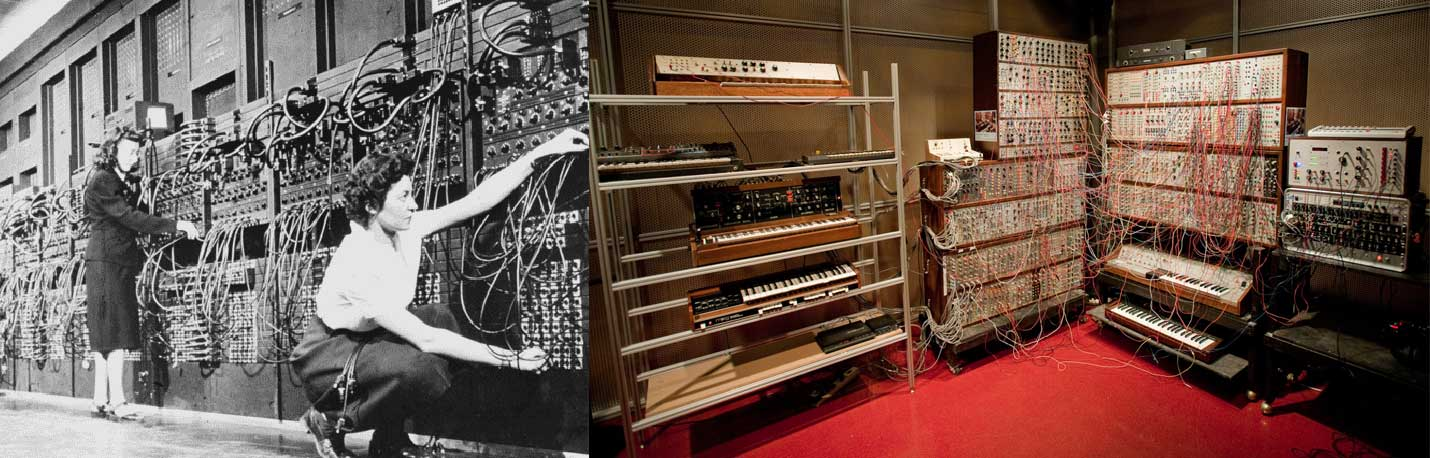
\includegraphics[width=1\linewidth]{pictures/analogicos}
    \end{center}
    \legend{Fonte: \cite{HayleyWilliams2015} e http://web.media.mit.edu/~joep/pics/ FullSynthMIT-Museum.jpg}
\end{figure}

As primeiras experiências musicais em computadores digitais foram realizadas na década de 50 por Max Mathews no Bell Telecom Lab. Para gerar os primeiros sons computadorizados, Max teve que desenvolver uma linguagem de programação própria, que chamou de \emph{Music I} \cite[253]{Holmes1985}. Depois de uma década desenvolvendo essa linguagem de programação musical, em 1968 passou a trabalhar no desenvolvimento do GROOVE ou \emph{General Real-time Output Operations on Voltage-controlled Equipment}, um equipamento que funcionava na plataforma \emph{Graphic 1}, ``um sistema computadorizado interativo que podia traduzir imagens desenhadas com uma caneta luminosa em uma tela'' \cite[253]{Holmes1985}, que era similar à plataforma utilizada por Ivan Sutherland no \emph{Sketchpad}. O GROOVE teve a primeira interface gráfica interativa para computação musical. 

\begin{figure}[ht]
    \caption{\label{max}Max Mathews e L. Rosler com a estação de trabalho Graphic 1. }
    \begin{center}
        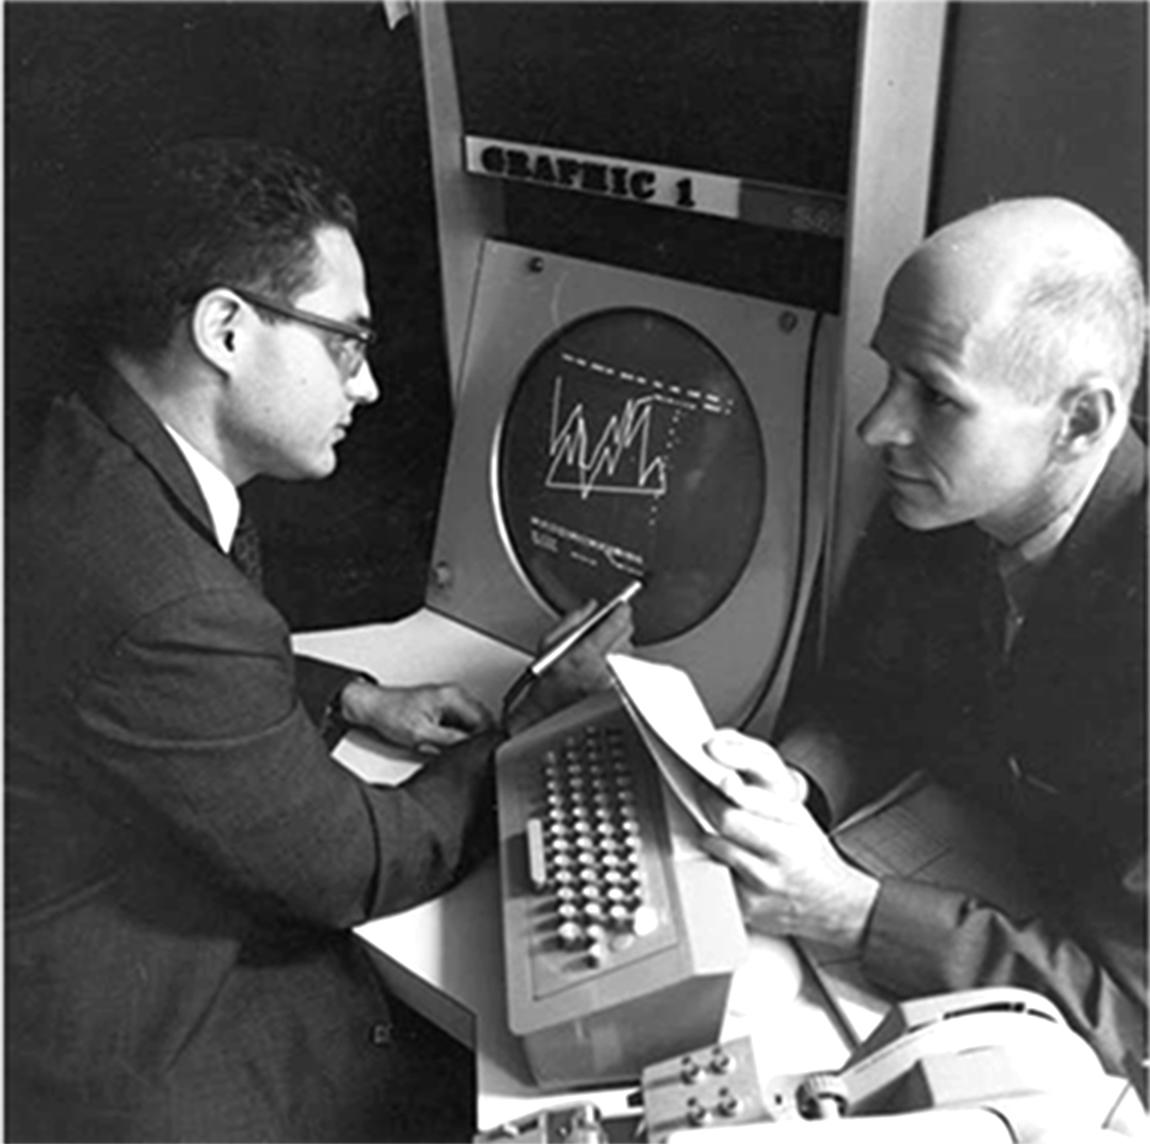
\includegraphics[width=0.5\linewidth]{pictures/MaxHolmes-251}
    \end{center}
    \legend{Fonte: Holmes, 1985 p. 251}
\end{figure}

Com o desenvolvimento da computação surgiram também novas formas de interação, como a alimentação e impressão de dados através de cartões perfurados e posteriormente o teletipo, um terminal parecido com o teclado dos computadores atuais, além da impressão de dados em tela por meio do tubo de raios catódicos. Com elas, a operação do computador não acontece mais no nível do hardware, e são desenvolvidas ``linguagens de programação mais eficiente e acessíveis'' (IAZZETTA, 1997 : 111). As próprias linguagens são interfaces que permitem a interação do programador com processos da máquina em um estágio mais bruto.

Até o final da década de 70, compositores precisavam trabalhar diretamente com programadores para realizar qualquer tipo de trabalho em computação musical. Foi o caso de James Tenney, que trabalhou com Mathews no Bell Telecom Lab para a composição de 6 peças ou o caso de Yannis Xenakis, que compôs \emph{Metastasis} quando teve acesso aos laboratórios da IBM em Paris\cite{Holmes1985}. Curtis Abbott, que escreveu o software da máquina 4C utilizada no final da década de 70 pelo IRCAN, começa seu artigo Music System Programming afirmando enfaticamente que ``programar é necessário para fazer qualquer coisa realmente nova em música computadorizada" \cite[51]{Roads1996}. A computação musical é um das vertentes desse campo que desponta na produção artística moderna, que Abbot já define como ``programação criativa'', um campo da computação que vai lidar com questões artísticas e estéticas. 

Na metade da década de 70, A New England Digital Corp. lançou comercialmente o primeiro sintetizador digital portátil, o Synclavier \cite[265]{Holmes1985}, com a interface que havia se tornado dominante entre os sintetizadores analógicos que dominavam o mercado, o teclado similar ao do piano \cite{JosephParadiso1998}. Com ele, a síntese digital era possível de ser acessada diretamente pelos músicos, através de sua interface familiar, mas apesar disso, seu preço na época estava entre \$200.000 e \$300.000 dólares, o que o tornava extremamente proibitivo. No começo da década de 80, já havia sido lançado também um sistema concorrente, o Fairlight CMI, que consistia em um sistema de processamento computadorizado, um monitor com caneta luminosa (lightpen), um teclado alfanumérico QWERTY, um teclado de 6 oitavas, além de um sistema de síntese analógica com 6 osciladores.

O Fairlight, apesar de mais acessível do que o Synclavier, era também um instrumento caro. Na época de seu lançamento o CMI original custava a partir de \$16.000 libras, o que não impediu que músicos famosos como Peter Gabriel, Kate Bush, Queen, Stevie Wonder, Herbie Hancock, Kraftwerk, Grace Jones, Frankie Goes To Hollywood, Thompson Twins, Human League, Tears for Fears entre outros o adotassem. \cite[18]{Twyman2004}(LEETE, 1999 e TWYMAN, 2004 : 18) O CMI era uma ferramenta atrativa tanto para engenheiros da computação, pelo processador sofisticado, quanto para compositores, que podiam utilizá-lo para fazer orquestração complexa de suas peças, quanto para músicos, que podiam utilizá-lo em estúdio ou em performances ao vivo. Mas não era uma ferramenta tão simples de se operar como anunciava. \cite[55]{Twyman2004}

Desde o lançamento do primeiro Macintosh, que tinha uma interface gráfica mais amigável, uma gama de softwares para a produção musical floresceu, voltadas para profissionais de música, desenvolvimento de jogos e performers. Em 1990, uma parceria entre a Digidesign, uma empresa que já desenvolvia softwares para produção musical e a Opcode, que era a maior fabricante de interfaces MIDI na década de 80 gerou o Studio Vision, que podia ser comprado por \$950 dólares e foi o primeiro a integrar gravação e edição de áudio e MIDI, sendo considerado o primeiro software do tipo digital audio workstation (DAW). Sua interface gráfica misturava conceitos desenvolvidos nos primeiros editores de áudio, como a representação do som através dos gráficos de amplitude por tempo, com um piano-roll, para marcação de notas em função do tempo. Isso ajudou a aproximar músicos que usavam editores de partitura digitais \cite{ChrisHalaby2011}. A interface de edição multipista permite gravar várias faixas e sobrepô-las paralelamente no espaço gráfico da tela, o que dá ao produtor musical a possibilidade de organização visual do fluxo sonoro ao longo do tempo, permitindo ajustes mais precisos de sincronização e mixagem.

No começo da década de 90, a tecnologia de gravação em disco rígido era extremamente cara e limitada, e as grandes empresas que dominavam o mercado de gravação em fita como a OTARI e a TASCAM não acreditavam que as pessoas iriam abandonar tão cedo as fitas magnéticas. Esse desinteresse permitiu que a Digidesign, que posteriormente veio se tornar a AVID, fosse se desenvolvendo continuamente e viesse a dominar o mercado de gravação digital até hoje, com as várias versões do Pro Tools que foram lançadas desde 1991 com sistemas integrados de hardware e software voltados para estúdios. Graças a uma placa de áudio que podia ser acoplada exteriormente ao Mac, o sistema de áudio permitia gravação multipista, processamento de sinal e sistema de mixagem sofisticados, que eram mais baratos que os sistemas de hardware disponíveis na época. (HALABY, 2011).

Para facilitar uma aproximação com os profissionais que já trabalhavam nos estúdios analógicos tradicionais, o sistema contava com uma interface gráfica de usuário que se apoiava na mímese do estúdio tradicional de gravação em fita. Assim, elementos familiares dos técnicos de estúdio foram copiados de uma maneira literal, sliders, displays luminosos, potenciômetros rotativos, botões de controle como play, pause e stop e somados ao modelo de interface de edição multipista desenvolvida no Studio Vision. 

Embora o discurso seja de uma revolução, na prática a interface se acomoda para ficar cada vez mais parecida ao estúdio tradicional. A cada versão do software lançada há um pequeno redesenho da interface gráfica, no sentido de acomodar mais recursos que são incluídos, mas também no sentido de tornar a interface mais “realista”, ou mais similar como imitação do estúdio de gravação analógica, com a inclusão de sombras, reflexos e degradés. Na figura abaixo, que mostra uma versão mais recente do software, podemos ver que os botões rotativos tem mais detalhes, como sombras e reflexos, e podemos ver também uma pequena tela similar à tela de um osciloscópio físico, que também possui um leve reflexo no canto superior esquerdo. Esses detalhes na prática não acrescentam nenhuma funcionalidade extra ao programa, na prática é possível que até prejudiquem, na medida que exigem gráficos mais pesados em termo de resolução e processamento gráfico, e nesse sentido servem somente para alimentar uma ideia de materialidade, dando ao software uma característica fantasiosa de objeto físico. 

Ferramentas como o ProTools, se enquadram no modelo que é chamado de \emph{Digital Audio Workstation} (DAW). DAWs são ferramentas que procuram emular de alguma maneira ferramentas do estúdio tradicional de fita, e como discuti no artigo ``Graphic Interfaces for Computer Music'' \cite{Stolfi2016}, tendem também a ter uma interface que busca mimetizar o equipamento de estúdio, em especial os controles giratórios e sliders, que são de difícil manipulação com mouse e teclados. Músicos profissionais no entanto, dispõe ainda em geral de uma série de equipamentos auxiliares para isso, como controladores MIDI, mesas de som automatizadas e toda uma gama de novas interfaces. O Pro Tools, por exemplo que foi por muitos anos um dos principais softwares de apoio aos estúdios tradicionais, era propagandeado como um sistema que integrado de hardware e software para produção musical. Sua interface imitava a tradicional mesa de mixagem de uma maneira quase literal, incorporando o desenho de amplitude de onda como forma de visualização padrão para os arquivos digitais como podemos ver na figura \ref{protools}, abaixo, retirada do site da empresa no início desta pesquisa.




\begin{figure}[ht]
    \caption{\label{protools}Interface do ProTools em 2015 }
    \begin{center}
        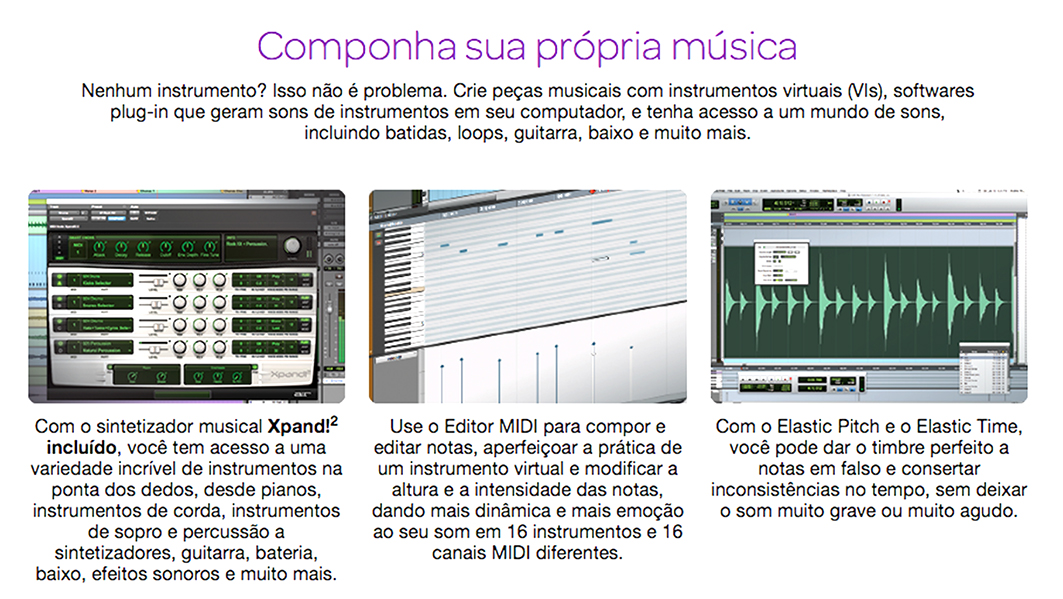
\includegraphics[width=1\linewidth]{pictures/protools}
        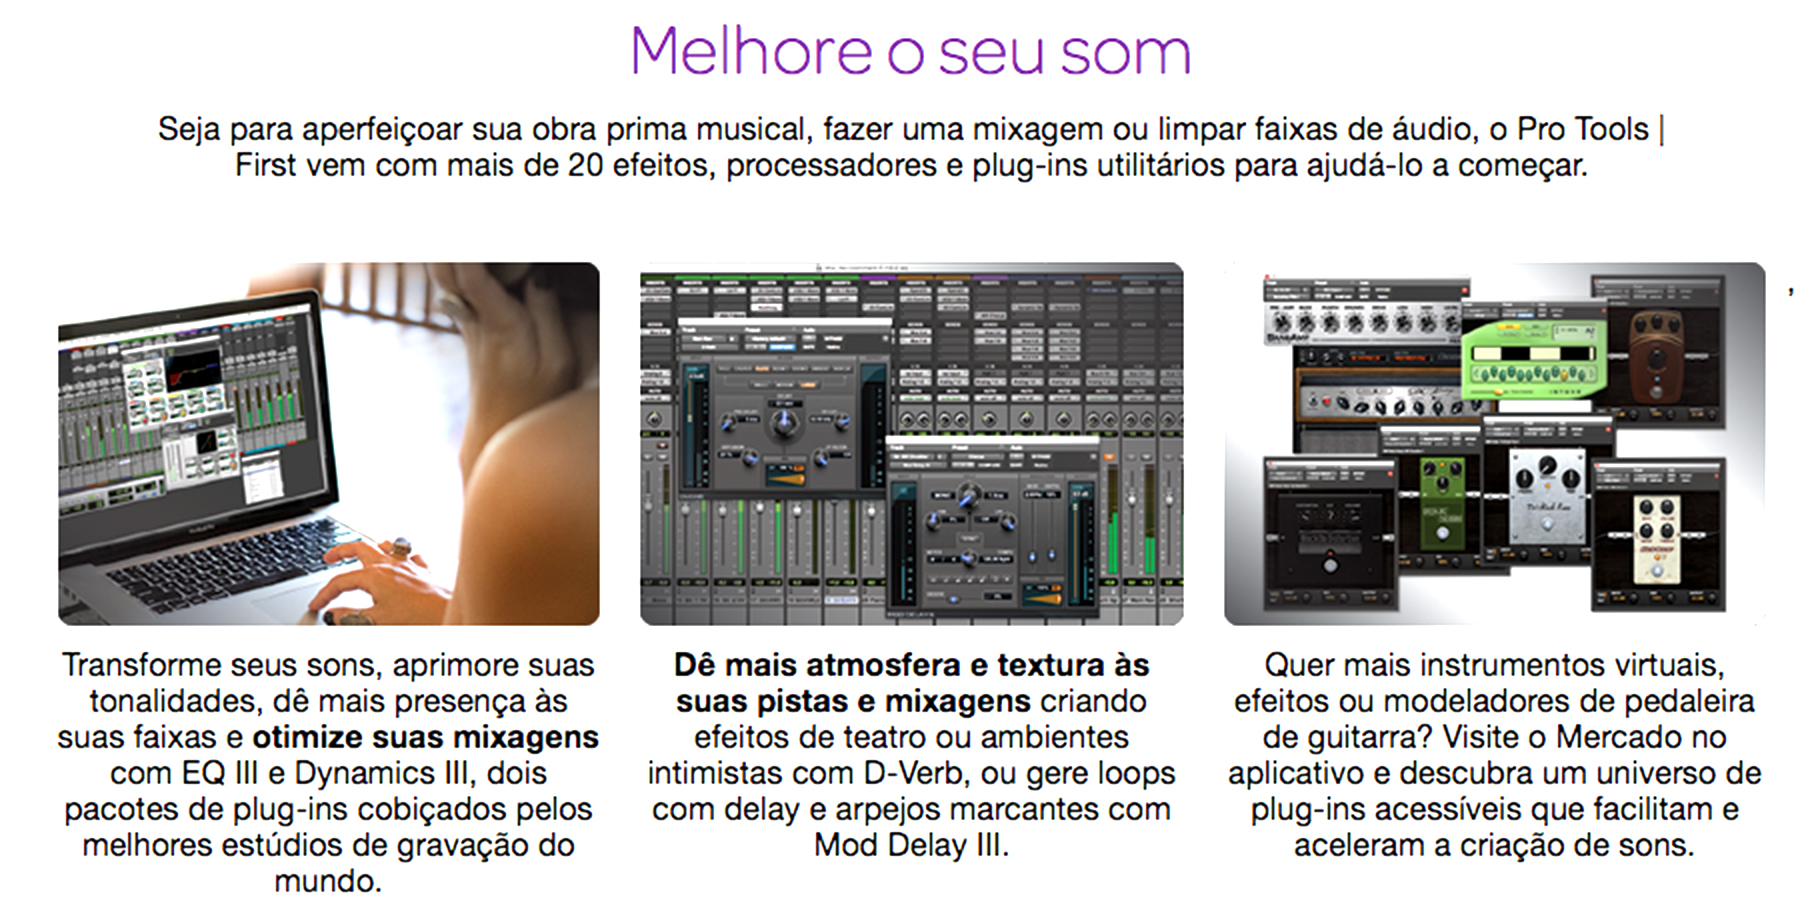
\includegraphics[width=1\linewidth]{pictures/protools2}
    \end{center}
    \legend{Fonte: Print Screen da Autora em 17 de dezembro de 2015. Site: https://www.avid.com/pro-tools-first}
\end{figure}

Outro paradigma de software voltado para produção musical é o dos programas que permitem ao usuário o design de suas próprias interfaces gráficas para controle de seus próprios aplicativos, como o Pd e o Max. Em 1986, Miller Puckette estava no IRCAN desenvolvendo um software chamado Patcher, um sistema gráfico para produção musical em tempo real para controlar a configurações de objetos no sistema MAX – um ambiente de programação orientada a objetos baseado em janelas voltado para produção musical, que na época rodava em um Macintosh, mas que já rodava no Synclavier II. O Patcher criava um sistema gráfico que simulava o sistema de cabos dos sintetizadores analógicos (figura 2) e mecanismos de abstração que permitiam condensar módulos criando entradas e saídas que poderiam ser conectadas entre si. Tratava-se na visão de Puckette, um sistema que permitiria que ``os músicos escolhessem em uma ampla gama de possibilidade, desenhando diagramas de fluxo de mensagem" \cite[5]{PucketteMiller}. 

\begin{figure}[ht]
    \caption{\label{patcher}À esquerda, um exemplo de patch feito no software Patcher de 1988, e à direita, objetos pré-programados e elementos de controle para configuração da interface gráfica.}
    \begin{center}
        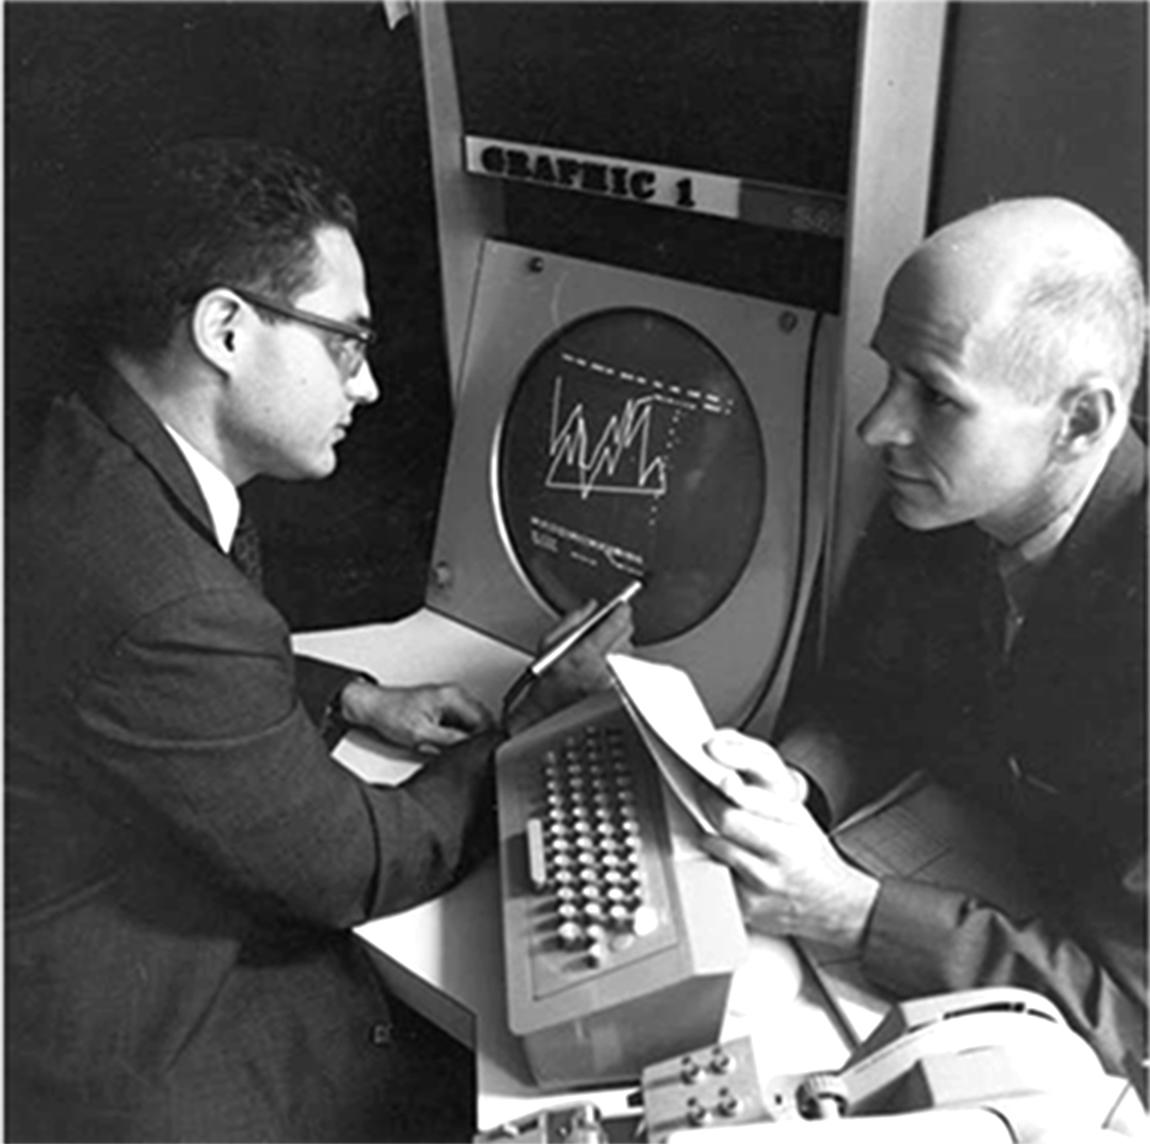
\includegraphics[width=0.5\linewidth]{pictures/MaxHolmes-251}
    \end{center}
    \legend{Fonte: \cite[6,9]{PucketteMiller}}
\end{figure}


Em 1990 o Patcher foi licenciado à Opcode e foi comercializado como Max\/Opcode, passando a ser desenvolvido por David Zicarelli. Em meados dos anos 90 a produção do software foi descontinuada pela Opcode, enquanto Miller Puckette continuou o desenvolvimento do programa no IRCAN que levou ao Max\/FTS (Faster than sound). Em 1996, Miller redesenhou totalmente o software e o lançou como um programa gratuito de código aberto chamado PureData (Pd), com uma interface gráfica muito semelhante à do Patcher original e das primeiras versões do Max. No ano seguinte, David Zicarelli fundou a Cycling 74, que continou o desenvolvimento e comercialização do Max\/MSP (abreviação tanto de Max Signal Processing ou de Miller S. Puckette) até os dias de hoje como software proprietário \cite{Cryer2018}.


Patchers, como o Pd e o Max, podem permitir a construção de interfaces complexas e adaptadas para necessidades específicas de músicos e artistas, mas possuem uma linguagem mais complexa e exigem um conhecimento especializado de quem as programa. O Pd apesar de apresentar essa modularidade também em uma metáfora de ``bancada para o design de instrumentos musicais eletrônicos para performance musical ao vivo", com objetos pré programados que podem ser conectados para que os artistas criem seus próprios instrumentos de acordo com necessidades específicas. \cite{PucketteMiller}
 
\begin{citacao}
Musicians can’t do much today without software, and so they are dependent on software developers. Software developers in turn are dependent on “users” (the musicians) to make artistic creations with their software; without that, the work of software development is pointless. The software developer strives to impose as few stylistic restrictions as possible on the musician. Yet every new generation of software that comes along reveals possibilities that were somehow not made possible, or at least not encouraged, by the previous generation. Soon we will learn that, no matter how general and powerful we believe today’s software to be, it was in fact steeped in tacit assumptions about music making that restrict the field of musical possibility. \cite{PucketteMiller}
\end{citacao}

\begin{citacao}
There is also a more subtle, and perhaps more fundamental, aim: to make it so that the software doesn’t impose one or another stylistic bias on the musician. Such a bias might be easy to spot (a built-in set of available time signatures or musical scales, for instance), or might be so ingrained as to be almost invisible (for example, Max’s and Pd’s orientation toward reactivity that seems to privilege some approaches to real-time performance over others).
\end{citacao}

\subsubsection{Interfaces para produção musical na web}
No primeiro ano desta pesquisa, além da pesquisa sobre interfaces gráficas para produção musical através de computadores, procuramos também estudar novas potencialidades que já surgiam utilizando a web como suporte.  fizemos um levantamento de experimentos organizados pelo site ``Chrome Experiments'' que reúne milhares de \emph{showcases} produzidos pela comunidade de ``programação criativa''\footnote{Disponível na url: \url{https://experiments.withgoogle.com/experiments}}. Em julho de 2016, apenas na categoria ``Sound and Music''""  haviam listados 138 experimentos. Entre experimentos estéticos com música generativa, jogos sonoros, videoclipes interativos, visualizadores de áudio, mixers e tocadores de MIDI, alguns podiam ser considerados instrumentos musicais. 

Entre eles encontramos vários exemplos de sintetizadores, samplers, processadores de áudio e sequenciadores, mas a maioria deles tinha como interface algo que mimetizava algum instrumento analógico ou eletrônico, principalmente o piano.

Encontrei algumas possibilidades interessantes como as experiências ``Lalo.li'' \footnote{Disponível em: <http://lalo.li/> }, que faz síntese de voz a partir de texto digitado na tela; ``Spectrogram and Oscillator''\footnote{Disponível em: <http://smus.com/spectrogram-and-oscillator/>}, que desenha um gráfico do espectro das frequências do som em tempo real a partir da entrada do microfone ou de um oscilador por clique ; Patatap\footnote{Disponível em: <http://patatap.com/ >}, uma espécie de bateria eletrônica audiovisual, que usa o teclado como input . Achei especialmente divertidas experiências multiusuário, como o Plink, onde cada pessoa que entra no site controlava um instrumento e vai tocando notas a partir de faixas verticais dispostas na tela (figura x) e o Multiplayer Piano\footnote{Disponível em: http://www.multiplayerpiano.com/}, um piano online aberto, que permite conexão através de midi, e tem um chat, onde diversos usuários podem tocar em uma jam coletiva ou conversarem enquanto ouvem alguém tocando.


\textbf{(ii) Instrumentos musicais online.} Nos últimos anos, principalmente depois do lançamento da Web Audio API, muitas pesquisas têm sido conduzidas no desenvolvimento de plataformas para tocar música na rede. Uma parte delas são baseadas em tipos existentes de instrumentos musicais digitais, como emuladores de DAW \cite{Jillings2017} ou sequenciadores \cite{Feenstra2016}.
\todo{incluir mais referencias aqui}

Essa diversidade de trabalhos demonstra o potencial das tecnologias web para o desenvolvimento de novas interfaces para produção musical, no entanto, a maioria dos instrumentos desenvolvidos até agora ou exigem um conhecimento prévio de técnicas musicais, ou são muitos simples e restritas em termos de expressividade musical \cite{Dobrian2006}. 


Apesar de mostraram que existe uma imensa potencialidade latente em explorar essas novas tecnologias, permitindo processos complexos de síntese de áudio e sampleamento, esses experimentos ainda são relativamente precários em termos de potencialidades de produção musical, se compararmos às ferramentas disponíveis para produção musical em software, como os chamados digital audio workstations (DAW) ou os patchers.

\end{otherlanguage*}


    % PARTE
    % \ifforcedinclude\else\part{Resultados}\fi

    % Primeiro capitulo de Resultados
    % The \phantomsection command is needed to create a link to a place in the document that is not a
% figure, equation, table, section, subsection, chapter, etc.
%
% When do I need to invoke \phantomsection?
% https://tex.stackexchange.com/questions/44088/when-do-i-need-to-invoke-phantomsection
\phantomsection


% Multiple-language document - babel - selectlanguage vs begin/end{otherlanguage}
% https://tex.stackexchange.com/questions/36526/multiple-language-document-babel-selectlanguage-vs-begin-endotherlanguage
\begin{otherlanguage*}{brazil}

    \chapter[Experimentos]{Experimentos}


    \begin{flushright}
         
    \end{flushright}

    % \newpage

\section{Primeiros Experimentos}

Partindo desta pesquisa inicial, procurei desenvolver alguns experimentos musicais iniciais.  Por um lado, haviam as tecnologias de programação, que estavam surgindo naquele momento, mas também havia um repertório e teorias da música que se colocavam com meu ingresso no Doutorado. Esses primeiros estudos que eram projetos bastante simples, foram importantes como exercícios estéticos e para começar um aprendizado dessas novas tecnologias.


\subsection{Bandas Críticas}
Bandas Críticas pode ser considera a primeira ``peça'' musical que escrevi. Até então, fazia apenas ``música''. Foi um primeiro exercício de escrita de uma partitura gráfica e o primeiro exercício de composição para uma equipe tocar. A peça foi composta a partir da proposta apresentada pelo Estúdio Fita Crepe \footnote{O Estúdio Fita Crepe foi um expaço dedicado à produção e performance de música experimental na cidade de São Paulo. \url{http://www.estudiofitacrepesp.com/}} de através do músico Ricardo Garcia ao NuSom, de um concerto de ``Música Silenciosa'', que seria uma ``música para acariciar os ouvidos'' que se embasaria em sutilezas de timbres e volumes.

A proposta foi de explorar metalinguisticamente o conceito de bandas críticas da audição, como apontamos em uma proposta de apresentação para o Simpósio Brasileiro de Computação Musical de 2015, que ocorreu em Campinas:


\begin{citacao}
A peça explora as frequências centrais e limítrofes das bandas críticas da audição, sobrepondo harmônicos e criando dissonâncias a partir de sons fora das escalas musicais tradicionais. Surge de um processo de composição metalinguístico, de investigar a própria percepção acústica, em um desejo de materialização de conceitos psicoacústicos em objetos sonoros.
Surge de um processo de composição metalinguístico, de investigar a própria percepção acústica, em um desejo de materialização dos conceitos psicoacústicos em objetos sonoros. No caso, representa uma materialização do conceito de bandas críticas, buscando explorar sensações audíveis e artefatos emergentes da exploração desse conceito. A performance é programada para 3 músicos, cada um conectado a uma caixa de som diferente, para enfatizar as diferenças entre as frequências exploradas. \cite{ArianeStolfi2015}
\end{citacao}

Também foi uma experiência de composição abstrata, a partida da idéia de buscar uma saturação sensória formada a partir de frequências puras mas não necessariamente harmônicas, que fosse estimular todas as regiões da cóclea. A peça é estruturada em quatro partes, um primeiro movimento introdutório onde os músicos não performam e o processamento acontece de forma automatizada pelo \emph{patch}, com todos os 44 osciladores ligando em um volume ascendente; num segundo momento, os músicos vão deligando os osciladores de acordo com uma ordem pré-estabelecidas, causando uma rarefação, até restarem apenas poucos osciladores ligados; na terceira parte os músicos improvisam a parti de harmônicos desses osciladores ligados; por fim, há um momento de ``destruição da onda'', onde os músicos passam a improvisar desenhando a onda, o que gera uma harmonia de ruídos, até a destruição completa dessas harmonias com a busca do silêncio.

Fizemos uma apresentação no Estúdio Fita Crepe, no evento ``Música? 11'', onde performaram junto comigo Davi Dontato e Sérgio Abdalla, no dia 29 de agosto de 2015 e outra no Simpósio Brasileiro de Computação Musical no dia 24 de novembro em Campinas, com a participação de Davi Donato e Luzilei Aliel. Análise do registro das gravações mostraram que o espectrograma da peça ficou bem próximo ao desenho da partitura pensado originalmente, como podemos ver na imagem \ref{bandasciticasspec}. 

\begin{figure}[htb]
    \caption{\label{bandasciticasspec}Spectrogramas gerados a partir das gravações da peça no Estúdio Fita Crepe (acima) e no SBCM (abaixo). }
    \begin{center}
    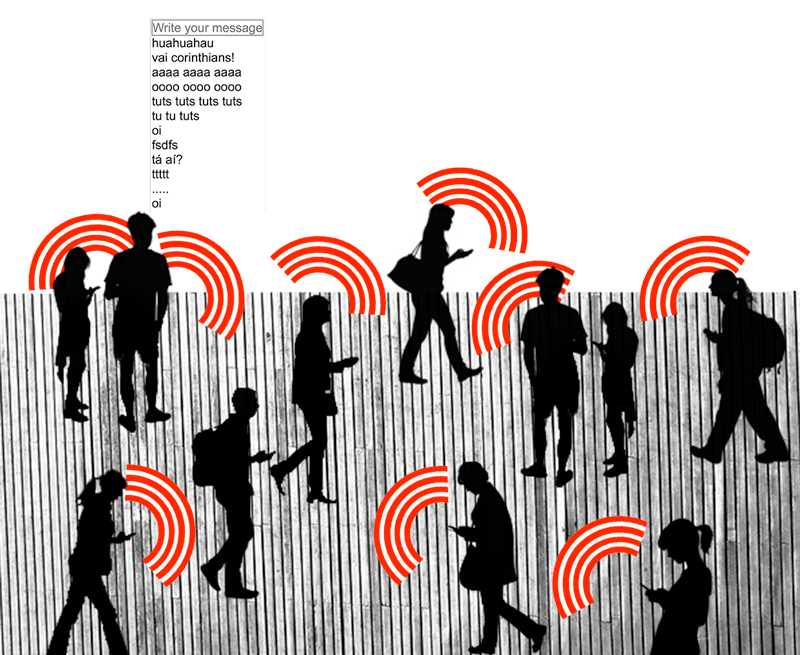
\includegraphics[width=1\linewidth]{pictures/banda_aberta_mob_crowd.png}
    \end{center}
    \legend{Fonte: Screenshot da autora, Janeiro de 2016}
\end{figure}



\subsection{QWERTY}
\label{sec:QWERTY}
Qwerty foi o primeiro experimento em web áudio desenvolvido após entrar no programa de doutorado. Como a idéia inicial do projeto era buscar formas de explorar os inputs dos computadores pessoais, partimos da principal forma de input que é o teclado QWERTY, que tem a disposição ainda das tradicionais máquinas de escrever. A idéia era transformar o teclado em uma máquina sonora, que não é em si uma coisa nova. O site Patatap, por exemplo, que mencionamos no capítulo anterior, é uma plataforma que funciona dessa maneira. Outro exemplo é o ``Typedrummer'' de Kyle Stetz \footnote{Disponível em: \url{http://typedrummer.com/}} , onde o usuário digita um texto, e para cada letra há um sample, e o texto é tocado em loop.


Para essa máquina, me inspirei nas leituras de Haroldo de Campos do seu poema épico Galáxias \cite{Campos2004}, que tem como estrutura um bloco contínuo de frases sinestésicas, sem qualquer tipo de pontuação ou espaçamento. 

Naquele momento, estava envolvida também no projeto de digitalização das revistas de poesia concreta Código \ref{codigo}, da revista de vanguarda lançada em 1973 e editada por Erthos Albino de Souza e Antônio Risério, que contém obras e traduções de vários poetas concretos desta geração. A revista Código, é como aponta Augusto de Campos ``acolheu materiais de vanguarda que não encontrariam guarida nas publicações convencionais alternativas" \cite{Scandurra2016}. Para a versão online da revista, para o qual programei a interface, seguindo uma idéia de design de navegação paratática, ou seja, que permitisse a re-combinação e re-montagem dos poemas de acordo com a vontade do leitor. Por conta deste projeto, estava em contato constante com as obras dos poetas desta geração, então partimos a pesquisa desta inspiração.

Parti do poema Galáxias porque ele é sobretudo extremamente sonoro. O livro acompanha um CD com as leituras de Haroldo de alguns fragmentos do seu texto, e foi de onde partimos para a extração dos primeiros samples, buscando uma atomização do discurso, em uma relação com a própria estrutura do poema, que como apontou o poeta Augusto de Campos em conversa com a autora, poderia ter tido sua primeira edição publicada em folhas soltas para ser recombinado, ideia que foi abandonada posteriormente.

\begin{figure}[htb]
    \caption{\label{codigo}Interface do site da digitalização da revista Código. }
    \begin{center}
    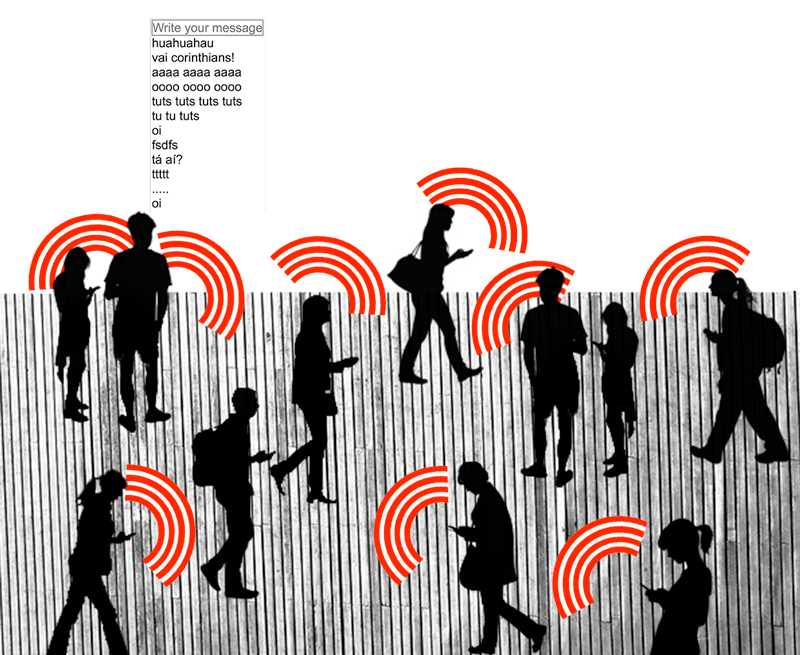
\includegraphics[width=1\linewidth]{pictures/banda_aberta_mob_crowd.png}
    \end{center}
    \legend{Fonte: Screenshot da autora, Janeiro de 2016}
\end{figure}

Partimos de um processo de escuta buscado encontrar os sons correspondentes a cada letra em forma de token nas leituras do poeta e fizemos um mapa onde cada letra digitada do teclado corresponde a um fonema relacionado, criando um sampler de 26 botões, que são disparados ao digitar.

A interface desenvolvida foi a mais enxuta possível (figura \ref{qwerty}), pensando em um minimalismo radical que se relaciona com a estética da poesia concreta, e também em uma idéia de brutalismo digital que defendemos nesta pesquisa.

\begin{figure}[htb]
    \caption{\label{qwerty}Interface do experimento Querty, com fragmento de texto do Galáxias digitado. }
    \begin{center}
    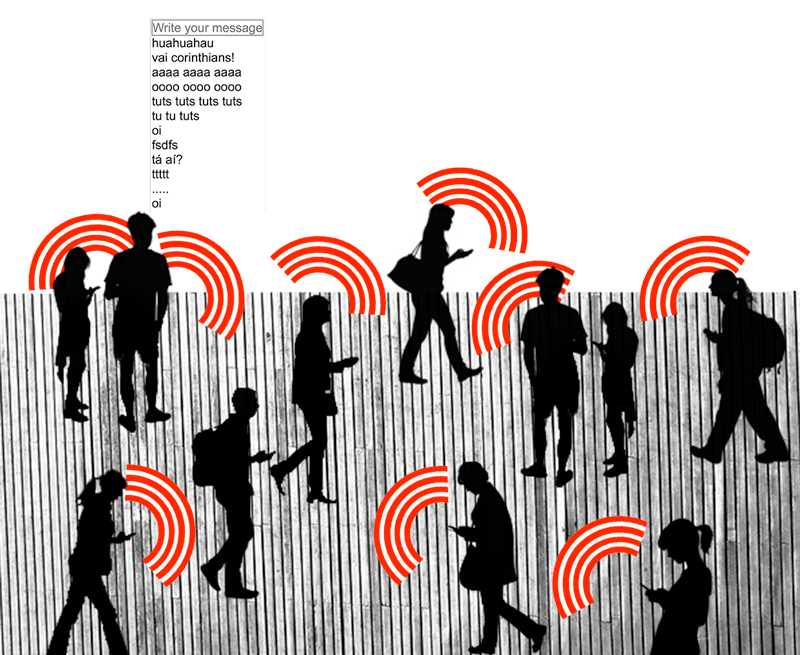
\includegraphics[width=1\linewidth]{pictures/banda_aberta_mob_crowd.png}
    \end{center}
    \legend{Fonte: Screenshot da autora, Janeiro de 2016}
\end{figure}





\subsection{Protesta Fora Temer}
Durante o mês de outubro de 2016, surgiu uma discussão na lista de emails da rede sonora sobre a possibilidade de se posicionar contra o impeachment da presidenta Dilma Rousseff, após uma breve discussão, verificou-se a dificuldade de elaborar um texto que fosse consenso entre as pessoas da rede, devido à ausência de um debate qualificado sobre o assunto e a divergência de opiniões políticas. 
Surgiu então a proposta de organizar um protesto sonoro, e foi lançado um pedido na lista, pela compositora Valéria Bonafé, para quem quisesse participar, que enviasse algum sample em mp3: 
\begin{citacao}
Conversei com algumas membras aqui da Sonora e propus que a gente organizasse um protesto-sonoro-fora-temer. Nossa ideia é montar um protesto sonoro colaborativo e interativo a partir de samples de áudio. O convite está aberto a todo mundo aqui da lista! Quem quiser participar basta enviar um (ou mais!) sample(s) de áudio. As indicações técnicas são apenas duas: que seja curto (questão de alguns segundos) e que esteja em MP3. A ideia é fazer algo leve (no sentido técnico) para não sobrecarregar o sistema de interação que vamos usar para articular esse banco de samples. Como relação ao conteúdo, a única coisa que combinamos é que o mot é “fora temer”. Mas também não precisa ser literal! Não é que precisa gravar apenas falando “fora temer”. Pode ser! Mas pode ser também algo em torno disso. Enfim, temos um tema. Mas cada um pode pensar algo a partir disso. O uso da criatividade, da imaginação, da exploração, da experimentação, da espontaneidade e tudo mais está em aberto! Assim como a “forma”. Pode ser uma gravação nua e crua, pode ser processada, por ser um recorte de algo etc. Enfim, a única diretriz de conteúdo é “fora temer” e a única diretriz técnica é “um sample curto e leve”.
\end{citacao}
Várias pessoas da lista mandaram contribuições e a partir do material enviado, e propus que fizéssemos, ao invés de uma faixa estática, um protesto sonoro interativo. Selecionei 25 samples de áudio e criei uma página html onde o movimento do mouse vai soltando aleatoriamente os samples cada vez que passa por cima de uma das palavras do site. O resultado pode ser uma massa de vozes – a maioria femininas – ou um coro protestante, dependendo da velocidade que o internauta percorre a página (figura \ref{protesta}). O site está disponível no endereço \url{http://www.sonora.me/protesta/foratemer/}. 

\begin{figure}[htb]
    \caption{\label{protesta}Protesta Sonora. }
    \begin{center}
    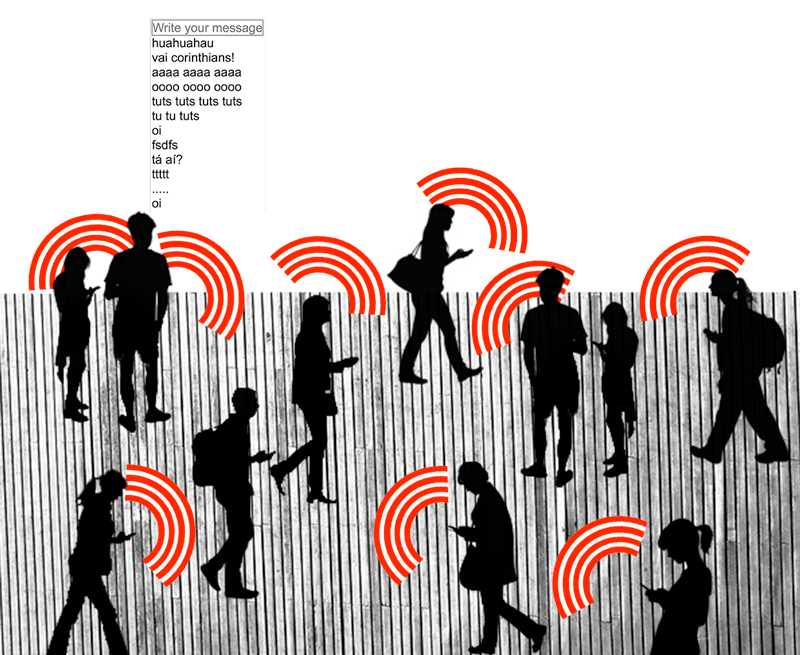
\includegraphics[width=1\linewidth]{pictures/banda_aberta_mob_crowd.png}
    \end{center}
    \legend{Fonte: Screenshot da autora dia 5 de janeiro de 2016}
\end{figure}



\section{Banda Aberta}
\begin{figure}[htb]
    \caption{\label{bandaabertamob}Banda aberta, imagem conceito para a proposta de intervenção pública}
    \begin{center}
    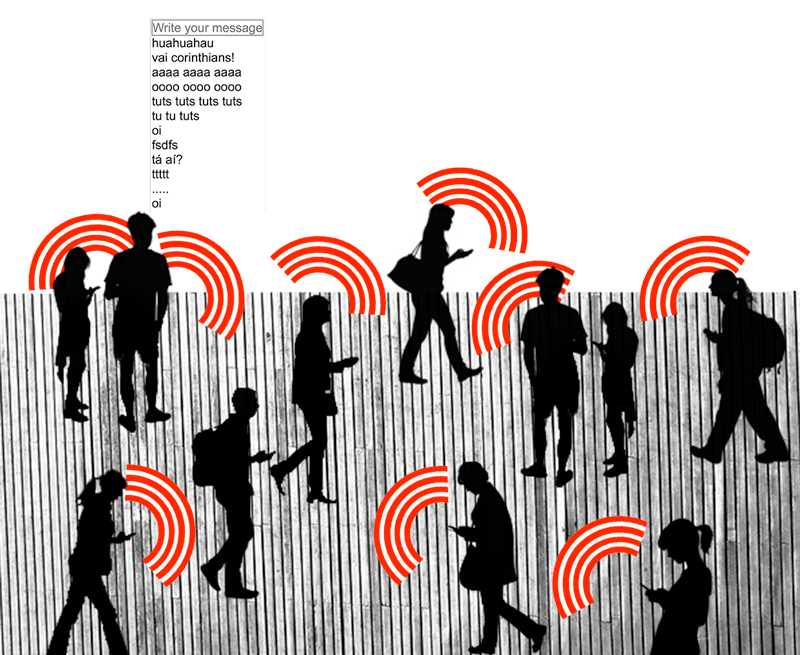
\includegraphics[width=1\linewidth]{pictures/banda_aberta_mob_crowd.png}
    \end{center}
    \legend{Fonte: desenho da autora}
\end{figure}

\subsection{Introdução}
O projeto Banda Aberta começou a ser desenvolvido como parte da proposta do NuSom para o Festival Bigorna na Praça, organizado pelo Estúdio Fita Crepe na praça José Molina. A ideia inicial era conectar os dispositivos pessoais das pessoas pela internet, de modo a potencializar os amplificadores individuais dos celulares e pensar em uma proposta de performance participativa que envolvesse a audiência. Foi o primeiro projeto realizado em parceria com outro programador, o engenheiro de computação Fábio Goródscy, que estava realizando mestrado na Computação musical no IME e o primeiro grande projeto desenvolvido no âmbito desta pesquisa. A parceria com um cientista da computação permitiu que desenvolvêssemos uma estrutura mais complexa do que a dos primeiros experimentos, que ainda eram baseados princialmente em HTML5, e partir para a exploração de recursos mais complexos da Web Audio API \cite{Adenot2015}.

O principal objetivo desta performance era o dar voz ao coletivo, liberdade de fala, criando possibilidades de comunicação musical sem significado. Visamos permitir que pessoas em um espaço público venham a interagir em um contexto musical, fazendo um espetáculo produzido por elas mesmas, sem necessidade de nenhum conhecimento musical, utilizando seus próprios celulares, via wifi através de um sistema \emph{open-source} de chat sonoro. A figura abaixo apresenta uma representação da performance em um ambiente aberto. 

Performance com participação da audiência mediada por tecnologia é um tópico emergente no campo da tecnologia musical \cite{wu2017open} e na esfera da arte contemporânea. Em contraste com performances tradicionais, onde há uma divisão estrita entre audiência e performer, as performances participativas tendem a diluir os limites entre a audiência e o performer \cite{kattwinkel2003audience}. 

Na tradição artística brasileira, esse assunto têm sido explorado desde os anos 60, principalmente no trabalho artístico de neoconcretos como Hélio Oiticica e Lígia Clark. Os parangolés de Oiticica, desenvolvidos a partir de um trabalho do artista com a comunidade da mangueira no final dos anos 60 eram peças vestíveis, cujo sentido se dava na dança e na manipulação das formas pela comunidade, assim como os Bichos, de Lígia Clark, que são esculturas articuladas que podem ser manipuladas e re-compostas pelo público. \cite{Braga2008}

Atualmente, o desenvolvimento da tecnologia trouxe novos recursos para facilitar e encorajar processos participativos em performances e instalações como: dispositivos computacionais portáteis como Arduino\footnote{Plataforma eletrôncia em código aberto Arduino: \url{https://www.arduino.cc/}} ou Bela{Plataforma para processamento de áudio de baixa latência Bela: \url{http://bela.io/}}; smartphones; sensores de dimensão reduzida e novas linguagens versáteis de alto nível como Python e JavaScript, que também ajudaram a criar as bases para o campo de pesquisa da computação ubíqua. Diversos projetos utilizam tecnologias deste tipo para o emprego criativo da participação da audiência em performances ao vivo, como os projetos massMobile \cite{Weitzner2012}, Mood Conductor \cite{Fazekas:2014}, Open Symphony \cite{wu2017open}, Crowd in Cloud \cite{Lee2016} e TweetDreams \cite{Dahl2011}. Em condições ideais, os participante são capazes de interagir durante as performances interferindo na narrativa de modo sensível. 

O projeto de ambientes colaborativos para produção musical pode ser desafiador, no sentido de que a audiência não necessariamente compartilha de domínio de técnicas e processos musicais. O projeto Banda Aberta é uma tentativa de explorar esse tema, usando a música como ponto de partida, pela função social que ela tem de comunhão e comunicação \cite{Koelsch:2014}. A idéia era de propor uma obra ``aberta'', como defendida por Umberto Eco \cite{Eco1991}, que, de acordo com Robey \cite{Eco1991}, requer do público um grau muito maior de envolvimento pessoal e colaboração do que qualquer obra de arte tradicional do passado. Segundo Eco, em uma obra aberta, ``é decisão do artista de deixar com que parte da organização de seus constituintes seja relegada ao público ou ao acaso, dando a elas assim não uma ordenação definitiva, mas uma multiplicidade de ordens possíveis" \cite{Eco1991}.

Com o projeto Banda Aberta, nós queríamos criar um sistema que pudesse ser facilmente utilizado como um instrumento musical pelos participantes, independente de qualquer conhecimento musical a priori. Existem vários tipos de interface para participação musical que partem de gestos de toque, simulando um processo de interação similar ao dos instrumentos tradicionais, como por exemplo a performance ``88 Fingers'' de Norbert Schnell e Benjamin Matuszewki \cite{Schnell2017}, onde cada participante pode controlar através do celular uma das teclas de um piano MIDI, ou ``Hyperconnected Action Painting", de Anna Xambó e Gerard Roma \cite{Xambo2017}, onde a audiência usa gestos com o celular para disparar sons pré definidos. Apesar de ambas serem divertidas como experiência participativa, o resultado sonoro nesses dois casos, na minha impressão pessoal, foi de uma massa de sons desordenada e fora de ritmo. Acredito que isso aconteceu em parte pela falta de prática em processos musicais coletivos por parte da audiência, que não necessariamente domina o gestual musical. Pensando nessa questão, queríamos propor uma ferramenta que pudesse ser acessada por qualquer usuário, independente de qualquer formação ou treinamento em práticas musicais, e para isso, procuramos partir de tecnologias que as pessoas já usam com mais desenvoltura.

\subsection{Descrição do Projeto}
Como já apontava McLuhan\cite{mcluhan1968comunicaccoes}, o alfabeto fonético é uma tecnologia fundamental para o desenvolvimento da cultura ocidental. Ele é fácil de se aprender e ajustável a várias linguages, sendo a sim, a base de toda cultura literata. Neste trabalho, nós fazemos uso do alfabeto como tecnologia para produzir música experimental. Texto e mensagens instantâneas se tornaram a principal forma de comunicação nos celulares hoje em dia, seja em comunicações síncronas ou assíncronas \cite{Madell:2007}, e por isso, decidimos experimentar com  o texto através de mensagens como forma de interação musical nesta primeira proposta. Muitos tipos de interfaces para produção musical usam o texto como forma de \emph{input}, como nos processos de \emph{live coding} \cite{Collins2003}, em processos participativos que usam feedback verbal da audiência \cite{noauthor_transglasphone_nodate}, em composições algorítmicas geradas por dados textuais ou sistemas que usam o teclado como controlador musical \cite{Fiebrink2007}. Neste projeto, nós procuramos criar um sistema que funcionasse para a produção musical de uma maneira análoga à relação entre o alfabeto e a linguagem oral.

A comunicação \emph{online} por texto se aproxima muito da comunicação oral, pela facilidade de escrita, e pela velocidade quase instantânea,\cite[33]{Levinson2001} Como aponta McLuhan, o conteúdo de um meio sempre agrega um meio anterior. O discurso, que é o meio mais antigo, está contido em quase todos meios subsequentes, como o livro, o telégrafo, o cinema e a televisão, e, é claro, a internet \cite[42]{Levinson2001}. 

McLuhan aponta que o espaço visual surge quando as consoantes foram criadas, ``como uma abstração sem significado", permitindo a análise das unidades silábicas em cada um de seus componentes. A consoante é para ele um não-som, algo que necessariamente ``soa junto". \cite[13-14]{mcluhan1968comunicaccoes} A base do discurso, segundo ele é o fonema, a unidade mínima do som, que seria a unidade mínima do som, na música, no entanto, Tenney  propõe em ``Meta-Hodos and Meta Hodos" o conceito de ``clang", que seria uma unidade \emph{gestalt} mínima reconhecível \cite[23]{Tenney1988}. 

Neste projeto, ao buscarmos o som das consoantes de um modo isolado, criamos uma desconstrução do discurso e procuramos reforçar esse caráter atomizante da linguagem escrita através de um duplo processo de conversão: discurso convertido em texto e posteriormente convertido em música.

A digitação é um processo muito mais simples para a maioria dos usuários de computadores e dispositivos digitais, em relação à operação de interfaces musicais, assim como a digitação na máquina de escrever era mais acessível para o homem comum do que o tocar de instrumentos analógicos. \cite[172]{Levinson2001}. Nossa ideia foi utilizar o \emph{input} de texto como forma de interação musical. 

Num projeto realizado previamente, o QWERTY, já tinha começado a explorar a digitação como forma de input, mapeando casa letra do teclado para um sample, que eram disparados de acordo com a digitação. Nós percebemos que isto exige do performer uma certa habilidade de controle do gesto, para que os sons saiam em um ritmo definido. Além disso, como as interfaces dos \emph{smartphones} não facilitam a digitação, queríamos pensar um sistema que não dependesse de agilidade para funcionar. Para encorajar a participação, nós projetamos um sistema que funcionava a partir de simples mensagens de texto.

No nosso projeto, utilizamos as frases como disparadores para uma sequência de samples, que são já compostos com durações fixas, num processo análogo ao de composição de frases musicais. Ao colocar um mecanismo de chat, as pessoas podem acessar o instrumento simultaneamente e participar de um diálogo sonoro. Conforme mais pessoas vão escrevendo simultaneamente, a camada de samples se torna mais densa e entrópica.

Diferente de processos de síntese vocal, nosso chat não concatena as sílabas, somente toca os sons pré-determinados em uma sequência, de modo que as palavras não são compreendidas como palavras, mas como frases musicais. Para adicionar um certo grau de controle à performance, utilizamos uma lógica da interface por linha de comando, através de certos comandos especiais que podem alterar a dinâmica da peça, ou alternar entre os conjuntos de samples compostos.

O projeto é construído a partir de dois dispositivos, o servidor de mensagens, que é programado em \emph{Ruby} e necessita de instalação em um servidor web, e a interface que faz o processamento das mensagens e é construída em HTML e \emph{JavaScript}  e funciona a partir da Web Audio API. O sistema está disponível como código aberto\footnote{O código fonte está disponível em: \url{https://github.com/fabiogoro/bandaserver}}   

\begin{figure}[htb]
    \caption{\label{bandaabertaserver}Diagrama esquemático dos servidores do projeto Banda Aberta}
    \begin{center}
        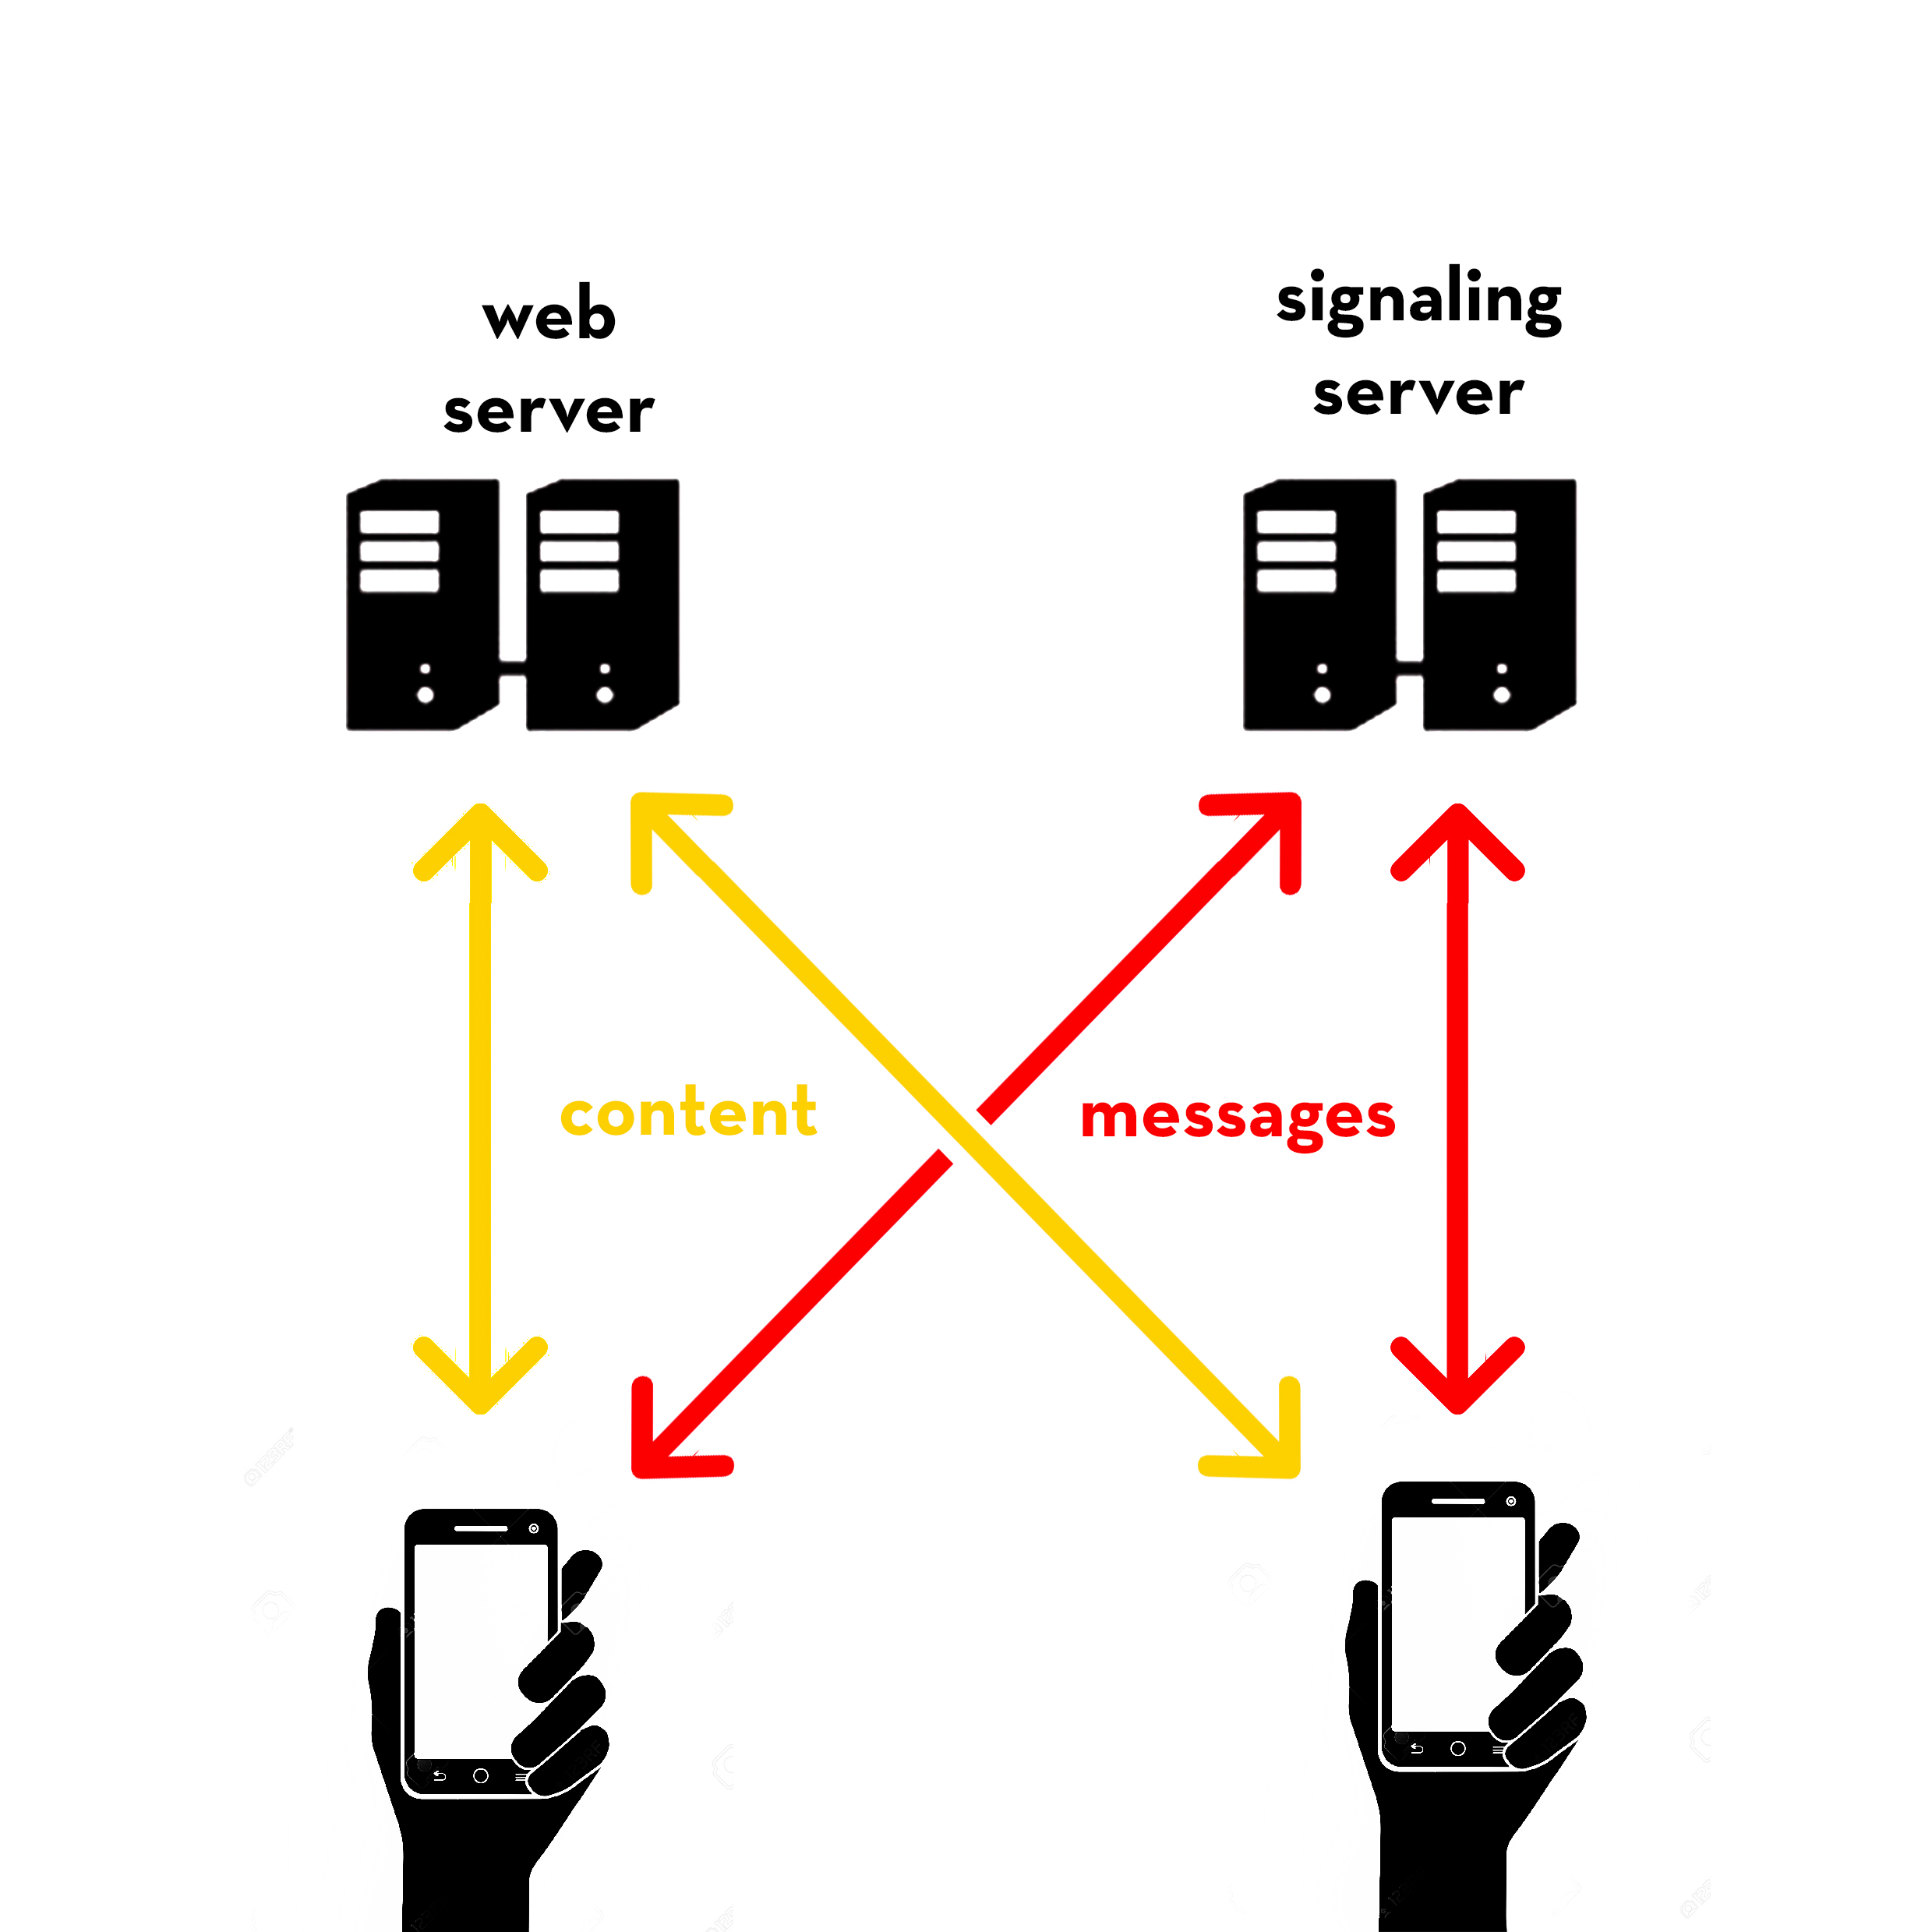
\includegraphics[width=0.5\linewidth]{pictures/server.jpg}
    \end{center}
    \legend{Fonte: desenho da autora}
\end{figure}

Na primeira versão, o processamento de áudio funciona somente por sampleamento. Os samples são numerados de acordo com a tabela ASCII e estabeleci um sample para caractere da tabela. O sistema converte as letras nos números equivalentes segundo a tabela, e toca o sample respectivo segundo a ordem estabelecida por cada frase que é enviada ao chat. Posteriormente, desenvolvemos também uma segunda versão baseada somente em síntese que também funciona da mesma forma, com um mapeamento um-para-um, de um som para cada letra.

\subsection{Desenvolvimento do Projeto}
Para o desenvolvimento do projeto Banda Aberta, adotamos ``Lean UX'' como metodologia de design. Lean UX é uma metologia ágil de desenvolvimento de software que tem sido aplicada em muitos projetos de webdesign \cite{leanux}. Envolve a criação de um protótipo mínimo e viável a partir de um estágio muito inicial do projeto. Este protótipo de vem então ser testado em condições reais de uso e melhorias são feitas de modo iterativo, baseando-se em observações e feedbacks recolhidos. O projeto foi desenvolvido como software de código aberto e está disponível no Github. \footnote{Os códigos-fonte do projeto estão disponíveis em: \url{https://github.com/fabiogoro/bandaserver}}. A arquitetura do sistema foi descrita com mais detalhes no artigo publicado na conferência Audio Mostly de 2017 ``Open Band: A Platform for Collective Sound Dialogues''~\cite{Stolfi2017}.

Nosso primeiro protótipo contava apenas com o conjunto inicial de samples nomeado de ``Galáxias'', e pudemos testa-lo menos de um mês após a proposta inicial em uma reunião do NuSom. Os samples utilizados nessa primeira versão eram os mesmos reunidos para o experimento QWERTY, descrito na seção \ref{sec:QWERTY}. A experiência foi registrada e fizemos uma análise dos comentários dos participantes\footnote{Registro da experiência pode ser visto em: \url{https://www.youtube.com/watch?v=Utc_4mT5b8s}}. Pudemos notar desde o princípio que a performance tinha um certo grau de ludicidade, pelas reações de riso e divertimento dos presentes. 


Neste primeiro teste em público, notamos que haviam alguns problemas com relação à compatibilidade de aparelhos, que foram posteriormente corrigidos. Recebemos também a opinião de alguns usuários que notaram que após alguns minutos a experiência sonora passava a ser um pouco entediante, com a repetição constante dos mesmos sons. Propusemos então a criação de outros bancos de sons, que seriam alternados durante a performance, e que um deles fosse criado colaborativamente por um grupo de estudantes da Universidade Anhembi Morumbi, orientados pelo professor Vítor Kisil,  que também apresentariam uma peça no Festival Bigorna. A partir daí, compusemos os demais pacotes de samples discutidos na seção \ref{sec:trad}

Nós queríamos assegurar a acessibilidade da audiência e garantir uma flexibilidade na montagem da performance, garantindo seu funcionamento mesmo em locais sem disponibilidade de acesso à Internet, o que era o caso do Festival Bigorna. Para isso, utilizamos um roteador Wifi para criar uma rede local aberta onde os usuários podiam ter acesso ao sistema em um servidor local (esta prática é frequentemente utilizada como estratégia para permitir a participação da audiência em sistemas de música móvel\cite{Lambert:2016}). Uma questão em performances participativas via celulares é que muitas vezes os usuários podem se distrair durante a se usar internet em dispositivos celulares para performances participativas e que usuários frequentemente podem se distrair por informações vindas de outros aplicativos como de trocas de mensagens ou redes sociais\cite{wu2017open}, e isto também é evitado pela rede local, que isola os usuários da internet, deixando os mais focados na performance e na experiência resultante. Durante as performances, os participantes acessavam o sistema através de um endereço IP que direcionava para uma máquina local com o servidor.

Nossa intenção era de que os participantes pudessem interagir com pouca ou nenhuma explicação anterior. No começo das era passada somente instruções de qual endereço acessar, onde havia a informação ``envie sua mensagem''. O endereço IP e o nome da rede eram informado em uma projeção na tela (na maioria das performances) para auxiliar os participantes a entrar mesmo depois do início da mesma. Um site com uma versão online é mantido no ar desde o lançamento do projeto e pode ser acessado no endereço: \url{banda.codigo.xyz}




\subsubsection{Tradução Inter Semiótica}
\label{sec:trad}

O uso do teclado do computador como \emph{input} para produzir sons em instrumentos musicais digitais pode ser relacionado muitas vezes com o teclado de piano. A maioria dos softwares do tipo DAW, como o ``Logic Audio" ou o ``Pro Tools" propõe uma interface de ``digitação musical" onde o teclado pode ser usado como um controlador MIDI precário (no sentido de que não possui sensibilidade à pressão) que relaciona teclas a notas musicais determinadas. Neste paradigma, a associação entre letras e sons é geralmente arbitrariamente determinada pela posição das teclas do teclado em comparação com a posição das teclas do piano, sem nenhuma relação semântica entre o som gerado e as próprias letras. Neste projeto, queríamos manter uma relação semântica entre as letras utilizadas nas mensagens e o resultado sonoro gerado. Para isso, buscamos algumas formas de tradução inter-semiótica entre os caracteres e os sons, que fosse além dessa analogia com as teclas de piano. A traduçnao semiótica é um procedimento utilizado para traduzir diferentes códigos, como aponta Plaza: 

\begin{citacao}
Na tradução intersemiótica como transcriação de formas o que se visa é penetrar pelas entranhas dos diferentes signos, buscando iluminar suas relações estruturais, pois são essas relações que mais interessam quando se trata de focalizar os procedimentos que regem a tradução. Traduzir criativamente é, sobretudo, inteligir estruturas que visam à transformação de formas. \cite[71]{JulioPlaza1969}
\end{citacao}

Aplicar um processo de tradução inter-semiótica de texto para som se relaciona com a idéia de áudio semântico \cite{Kostek:2010}, mas não no sentido tradicional, já que o objetivo aqui não foi o de dar sentido semântico aos sons, mas sim o de explorar quais poderiam ser os significados das letras quando essas fossem transformadas em sons. A abordagem foi de produzir os samples de acordo com o conceito de James Tenney \cite{Tenney1988} de Clang, ou ``gestalt aural", que é similar ao conceito de objeto celular de Pierre Schaeffer, que são objetos sonoros breves ou redundantes \cite{Chion1983}. A ideia foi pensar em átomos que pudessem ser recombinados livremente na medida em que as mensagens fossem escritas. Este procedimento aumenta as possibilidades paratáticas do sistema ao permitir re-combinações para além das possibilitadas pela linguagem escrita.


No sistema fonético, Schaeffer \cite{Schaeffer2007} aponta que as vogais em geral servem como sons de suporte e as consoantes como articulação. Segui esse princípio guia para o mapeamento das letras em sons, buscando cobrir uma grande variação de ``clangs", para deixar espaço para o acaso. Para a primeira versão do projeto, foram feitos 4 grupos de samples com sonoridades diferentes que podem ser mudados em tempo real por quem souber os comandos especiais: 

\begin{description}
 \item[Galáxias] A primeira estratégia foi de construir um alfabeto sonoro, usando processo de analogia com os sons do alfabeto fonético. Apesar de existirem muitos sistemas de síntese de discurso, a tentativa foi de isolar os sons, atomizando o discurso e consequentemente, o transformando em música através do encadeamento sucessivo de sons em uma estrutura rítmica. 
Em uma homenagem à poesia concreta, como definida por Augusto de Campos: ``tensão de palaras-coisas no espaço-tempo'' \cite[45]{campos_teoria_2014}, começamos a samplear os sons desse alfabeto das leituras de Haroldo de Campos do Poema Galáxias \cite{Campos2004}, um poema épico longo que se situa entre a prosa e a poesia, com várias páginas de texto sem nenhuma divisão de parágrafos ou marcas de pontuação. Sua leitura calma e grave foi percebida como uma fonte rica para um conjunto consistente de sons, e dessas gravações conseguimos extrair um conjunto que cobriu todas as letras em caixa baixa. Para as letras maiúsculas, procurei buscar sons mais poderosos, parte dos quais retirei de uma demonstração de técnicas vocais estendidas gravada por Stênio Biazon e outros que gravei especialmente para isso usando minha própria voz.  

Para os caracteres, a relação direta entre os sons e os samples não é tão clara, uma vez que não são represantações fonéticas, então optei por procurar outras relações possíveis bem como outras fontes de sons. Em alguns casos seguimos uma lógica de relação mais simbólica, como de caixa registradora para o signo \$ e em outros, associações mais icônicas, utilizando uma técnica de síntese subtrativa por corte visual de espectro. Este é o conjunto padrão de samples, e é usado como introdução para tornar as pessoas familiares com o sistema de associação. Exemplos deste pacote de sons podem ser ouvidos em: \url{http://spectro.codigo.xyz/spectrogramplayer/}

\begin{figure}[htb]
    \caption{\label{samplesgalaxias}Espectrogramas do Conjunto de Samples Galáxias}
    \begin{center}
        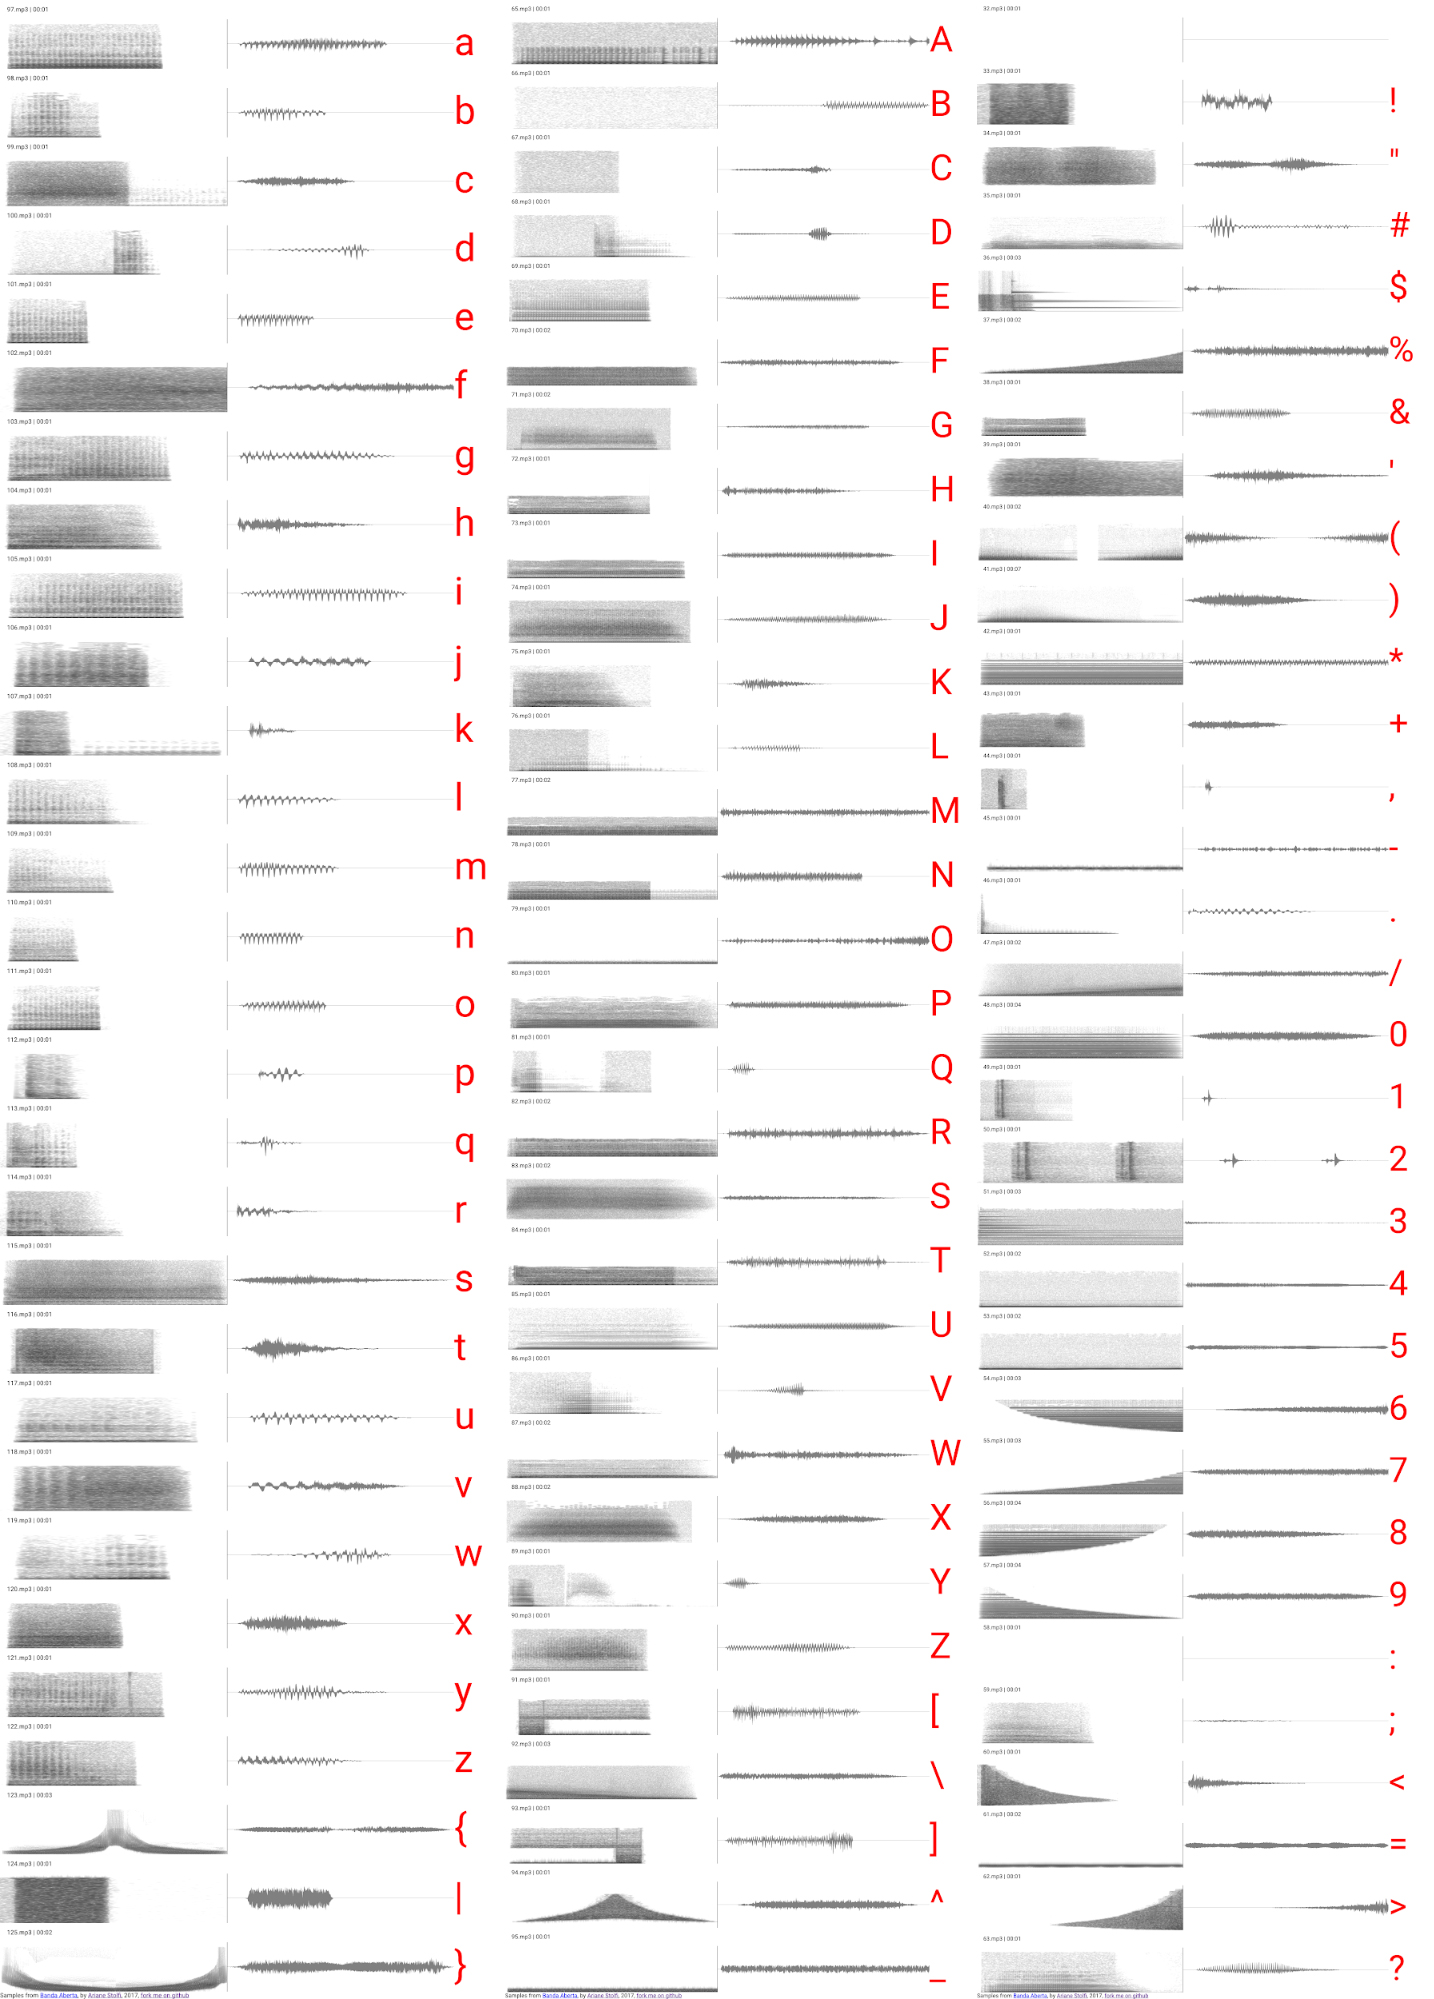
\includegraphics[width=0.7\linewidth]{pictures/cap3/bandagalaxias.jpg}
    \end{center}
    \legend{Fonte: screenshot da autora}
\end{figure}


\item[Percussão e Acordes] Para o segundo conjunto de samples, procurei lidar com materiais mais tradicionais do repertório da música popular eletrônica, como samples de percussão e acordes de sintetizadores extraídos de bancos de samples. Para manter uma estrutura lógica coerente na relação entre sons e letras, sons percussivos foram empregados no papel de articulação (nas consoantes) e acordes de sons contínuos como suporte (nas vogais). Nesta experiência, usamos uma progressão de Dó maior para a composição dos acordes das vogais, com samples gerados por síntese aditiva, e para as letras maiúsculas utilizamos um timbre com mais harmônicos do que os das letras em caixa baixa. \footnote{Exemplos deste pacote podem ser ouvidos em: \url{http://spectro.codigo.xyz/spectrogramplayer/perc.html} }
A associação entre as consoantes e os sons percussivos foi feita através de uma escuta reduzida de uma coleção grande de samples, buscando identificar sons que lembrassem características fonéticas das letras originais, como um bumbo para a letra ``B'' e pratos para ``S''. Mais uma vez aqui, fizemos essa associação mais direta entre sons e fonemas nos caracteres do alfabeto, enquanto para os caracteres especiais procuramos outras relações, como por exemplo entre sua forma visual e o desenho espectral dos sons. Alguns caracteres especiais foram extraídos da peça de Velimir Khleibnikov ``Radio of the Future''\footnote{Disponível em: \url{http://www.ubu.com/sound/russian_avant.html}}.

\begin{figure}[htb]
    \caption{\label{samplespercussao}Espectrogramas do Conjunto de Samples Percussão e Acordes}
    \begin{center}
        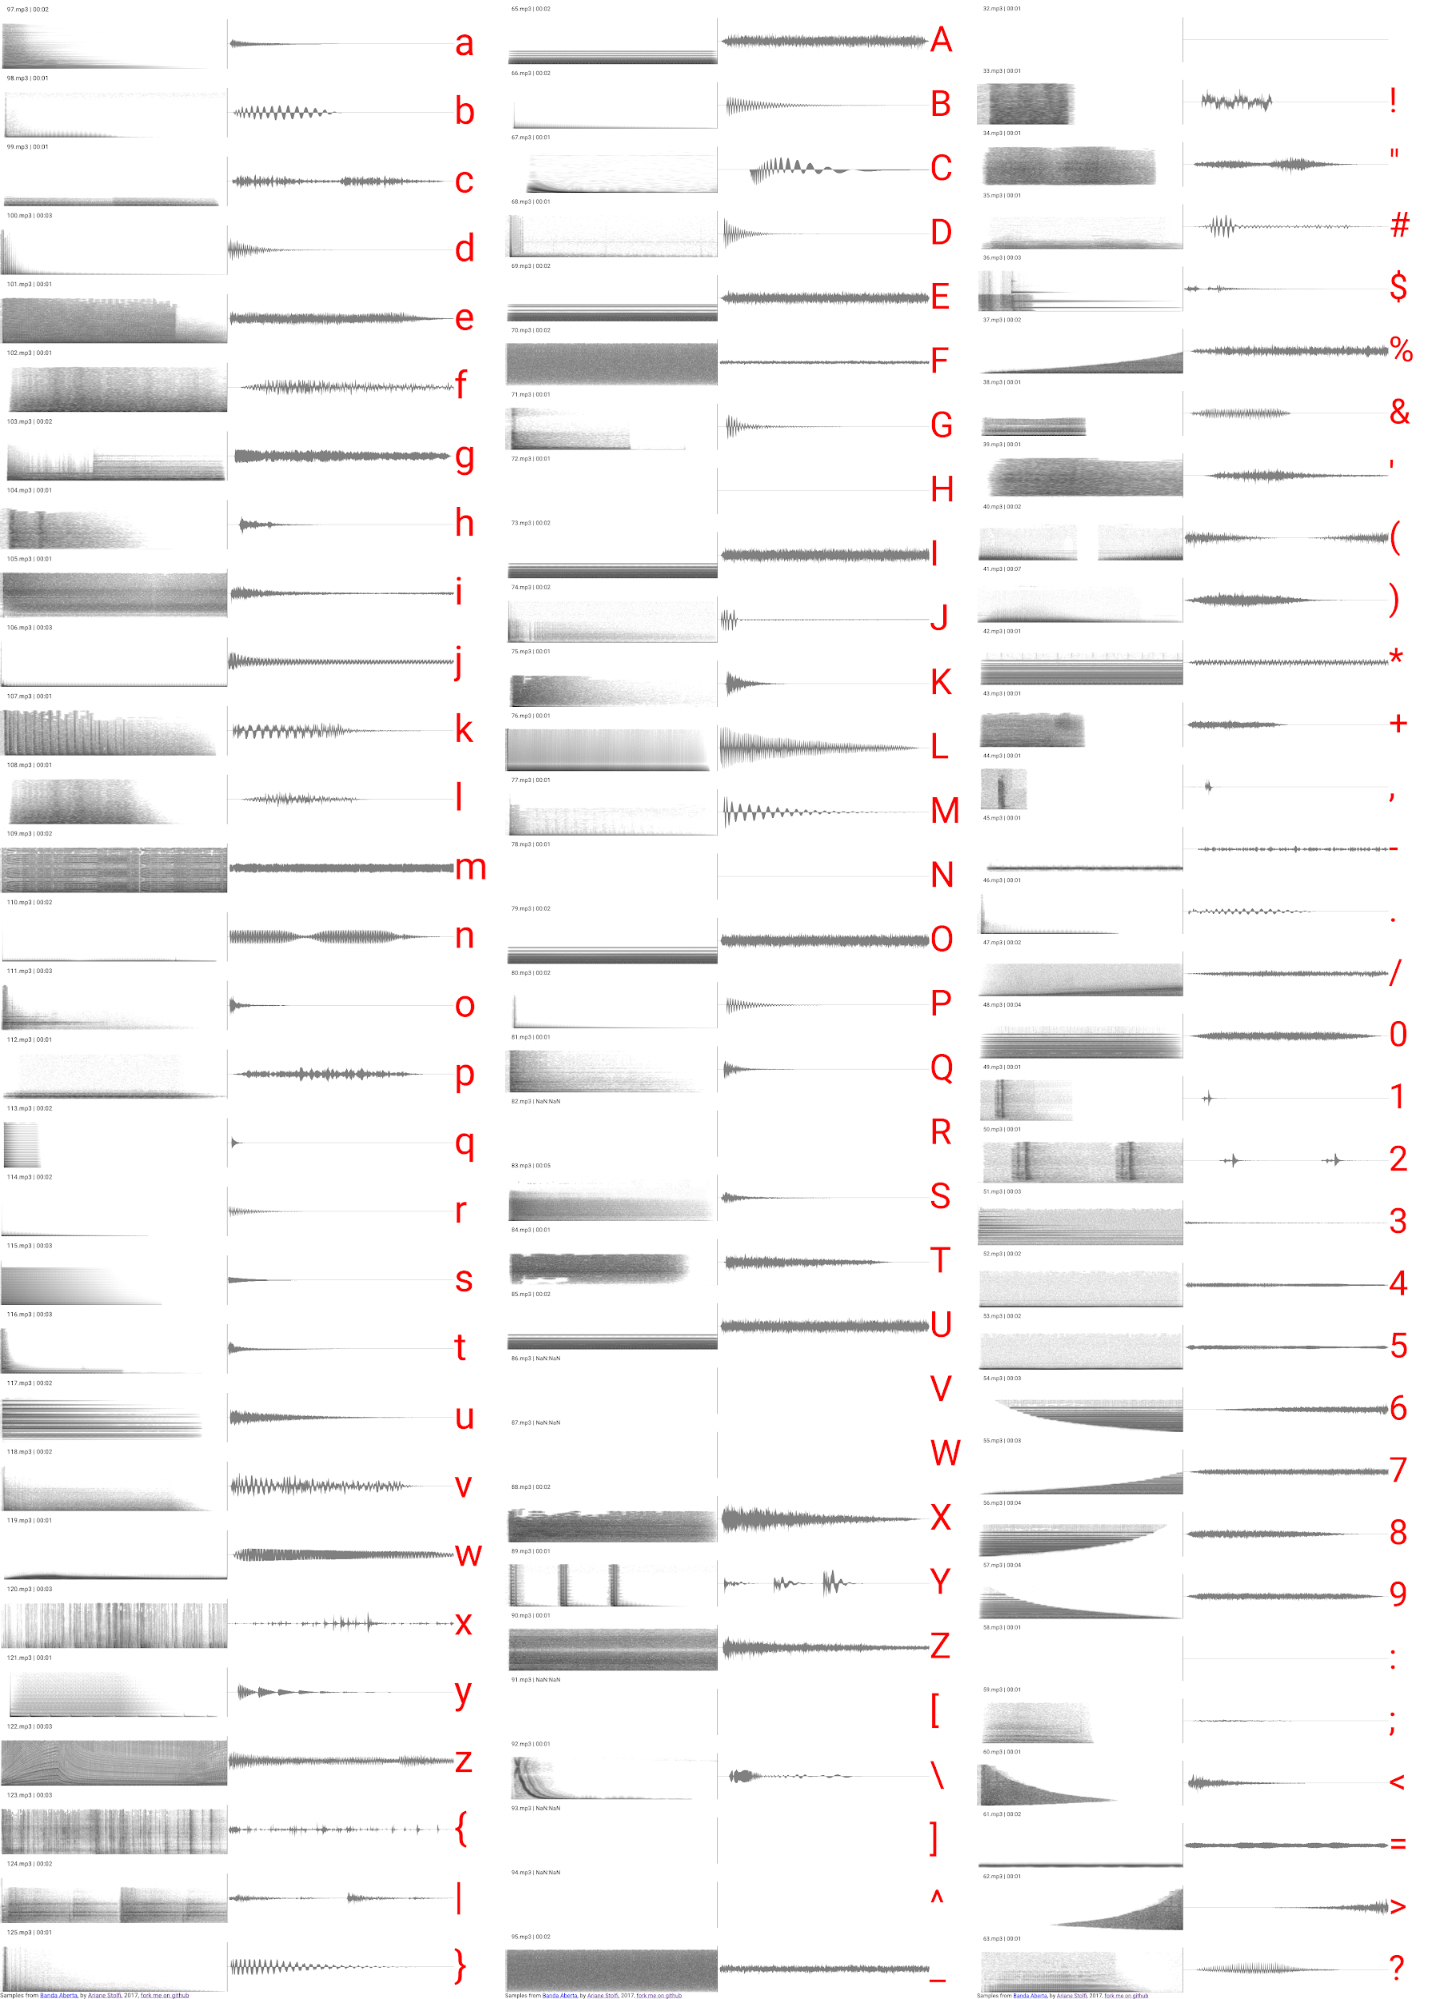
\includegraphics[width=0.7\linewidth]{pictures/cap3/bandapercussao.jpg}
    \end{center}
    \legend{Fonte: screenshot da autora}
\end{figure}

\item[Pacote Colaborativo]O terceiro conjunto de samples foi montado a partir da colaboração de alunos da turma de Produção Musical da Unviersidade Anhembi Morumbi, sob orientação do professor Viktor Kisil, que solicitou da turma samples para a composição deste conjunto de sons. Este pacote contém samples de fontes sonoras muito variadas, de concretos a sintetizados. A associação entre letras e sons não foi feita procurando analogias como nos outros conjuntos, e sendo assim, ele provém sons mais excêntricos. \footnote{Exemplos podem ser ouvidos em: \url{http://spectro.codigo.xyz/spectrogramplayer/fx.html}} 

\begin{figure}[htb]
    \caption{\label{samplescolab}Espectrogramas do Conjunto de Samples Colaborativo}
    \begin{center}
        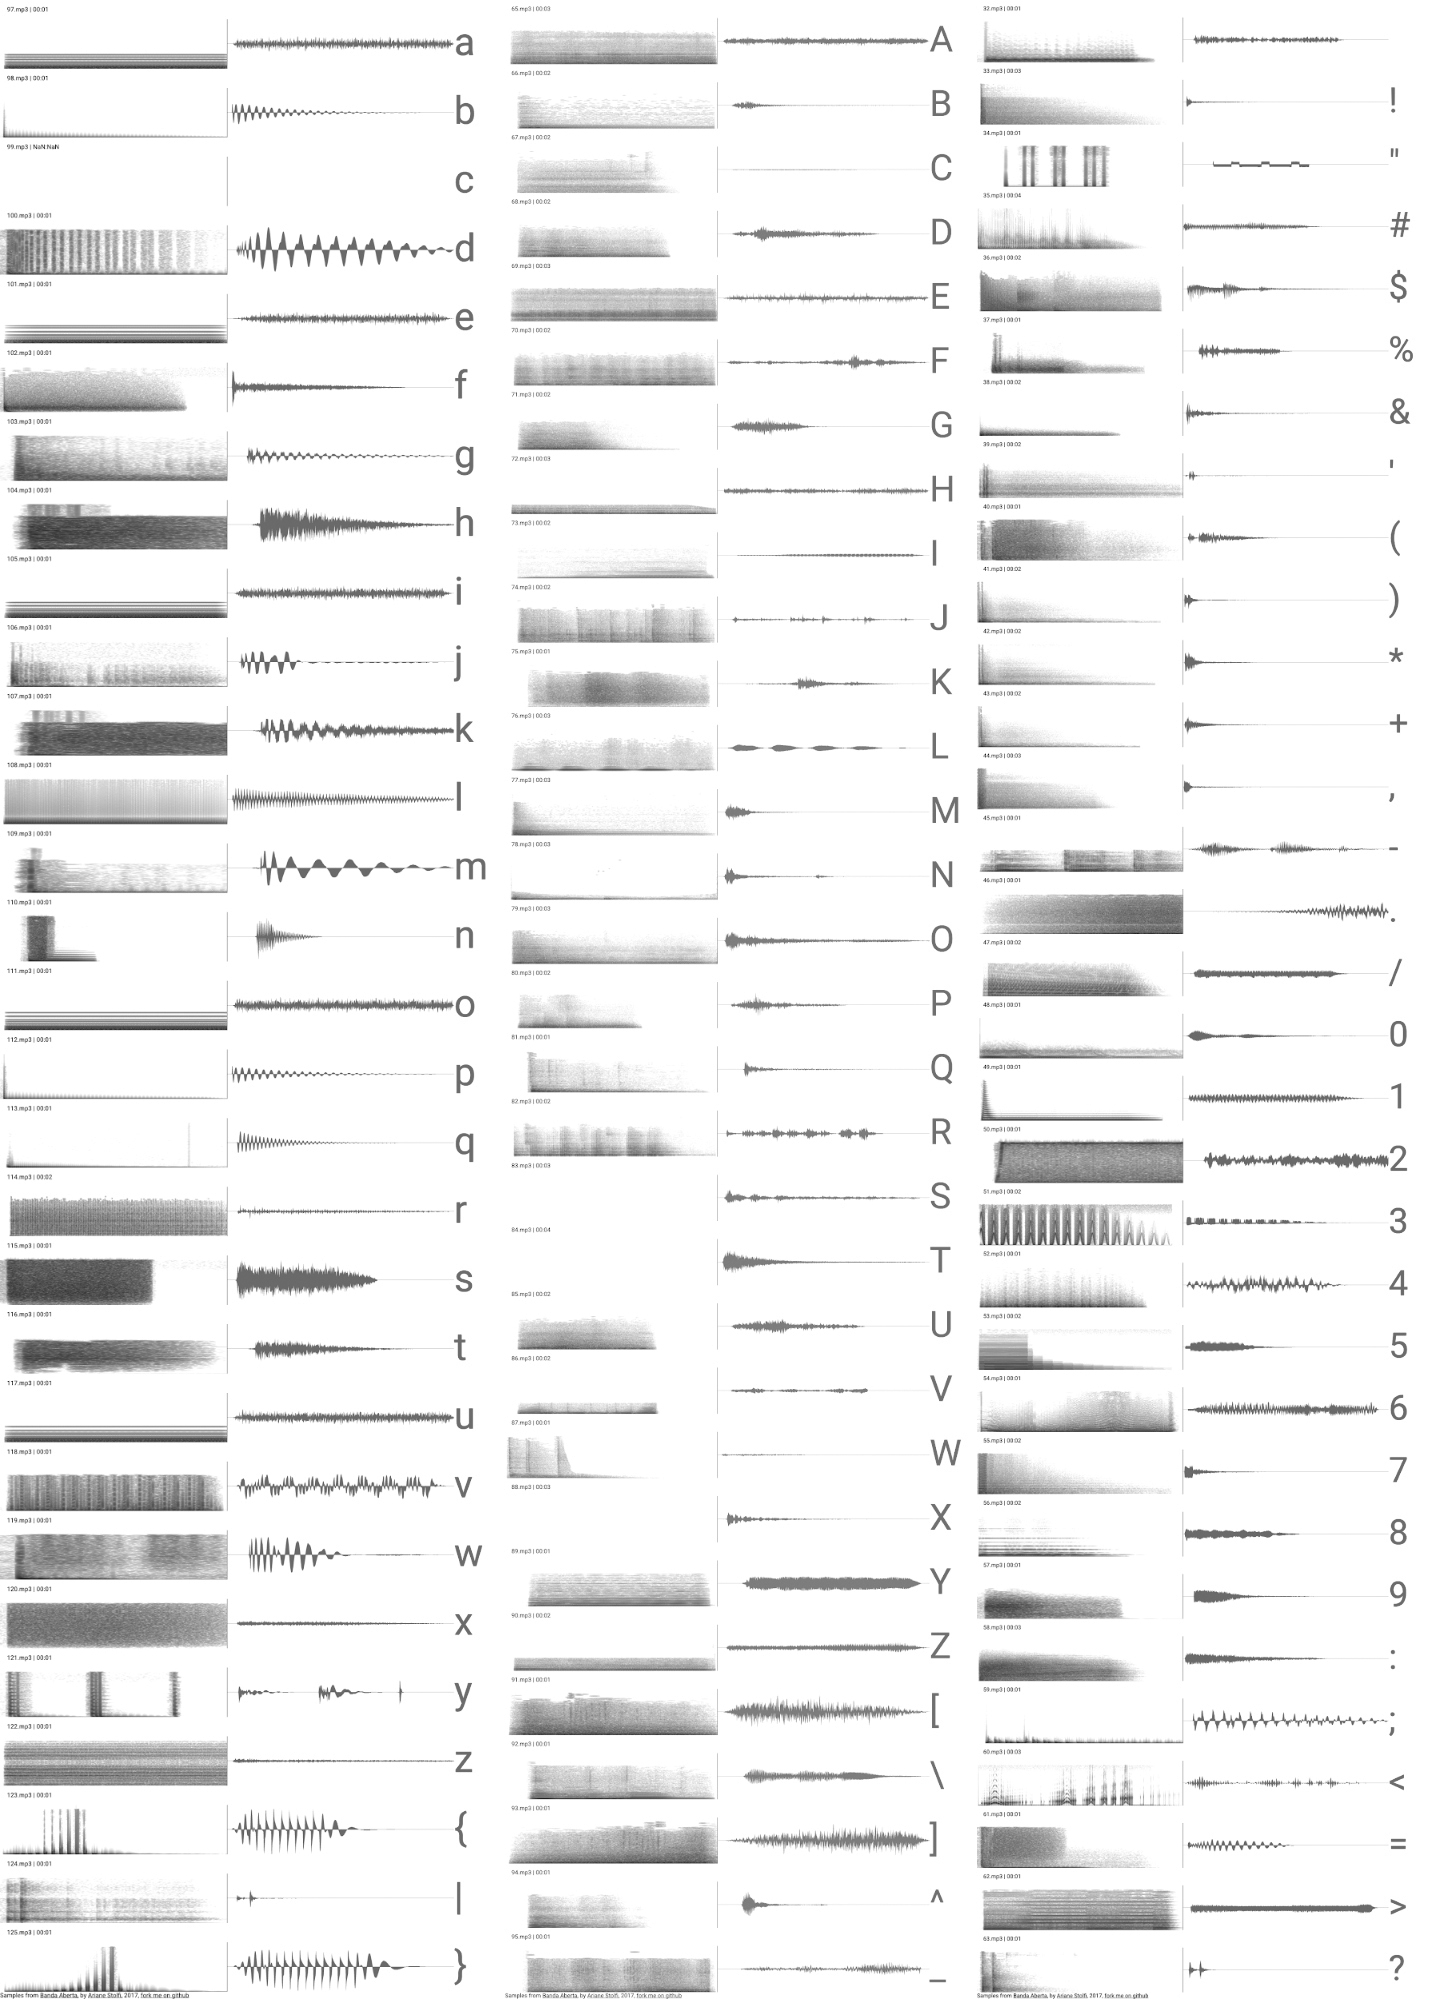
\includegraphics[width=0.7\linewidth]{pictures/cap3/bandaabertacolab.jpg}
    \end{center}
    \legend{Fonte: screenshot da autora}
\end{figure}

\item[Orquestra Errante] O quarto conjunto é formado por samples recortados de gravações de sessões de improvisação musical da Orquestra Errante, conduzida pelo professor Rogério Costa. Eles foram produzidos em sua maioria por instrumentos acústicos, como saxofone, flauta, piano, trombone, contrabaixo, percussão e voz. As gravações base que utilizei foram feitas durante ensaios da orquestra no estúdio do CMU, muitas vezes utilizando técnicas estendidas. Nós obtivemos um arquivo com várias gravações passadas desses ensaios, e empregamos técnicas de escuta reduzida e análise espectrográfica pra identificar ``clangs" que pudessem ser isolados para funcionar como átomos. Aqui novamente aplicamos uma analogia entre os fonemas e os sons sampleados e as funções de articulação para as consoantes e de suporte para as vogais. Para os numerais, usamos analogia entre batimentos e a quantidade representada. Exemplos deste conjunto podem ser ouvidos em: \url{http://spectro.codigo.xyz/spectrogramplayer/orquestra.html}
\end{description}

\begin{figure}[htb]
    \caption{\label{samplesorquestra}Espectrogramas do Conjunto de Samples Orquestra Errante}
    \begin{center}
        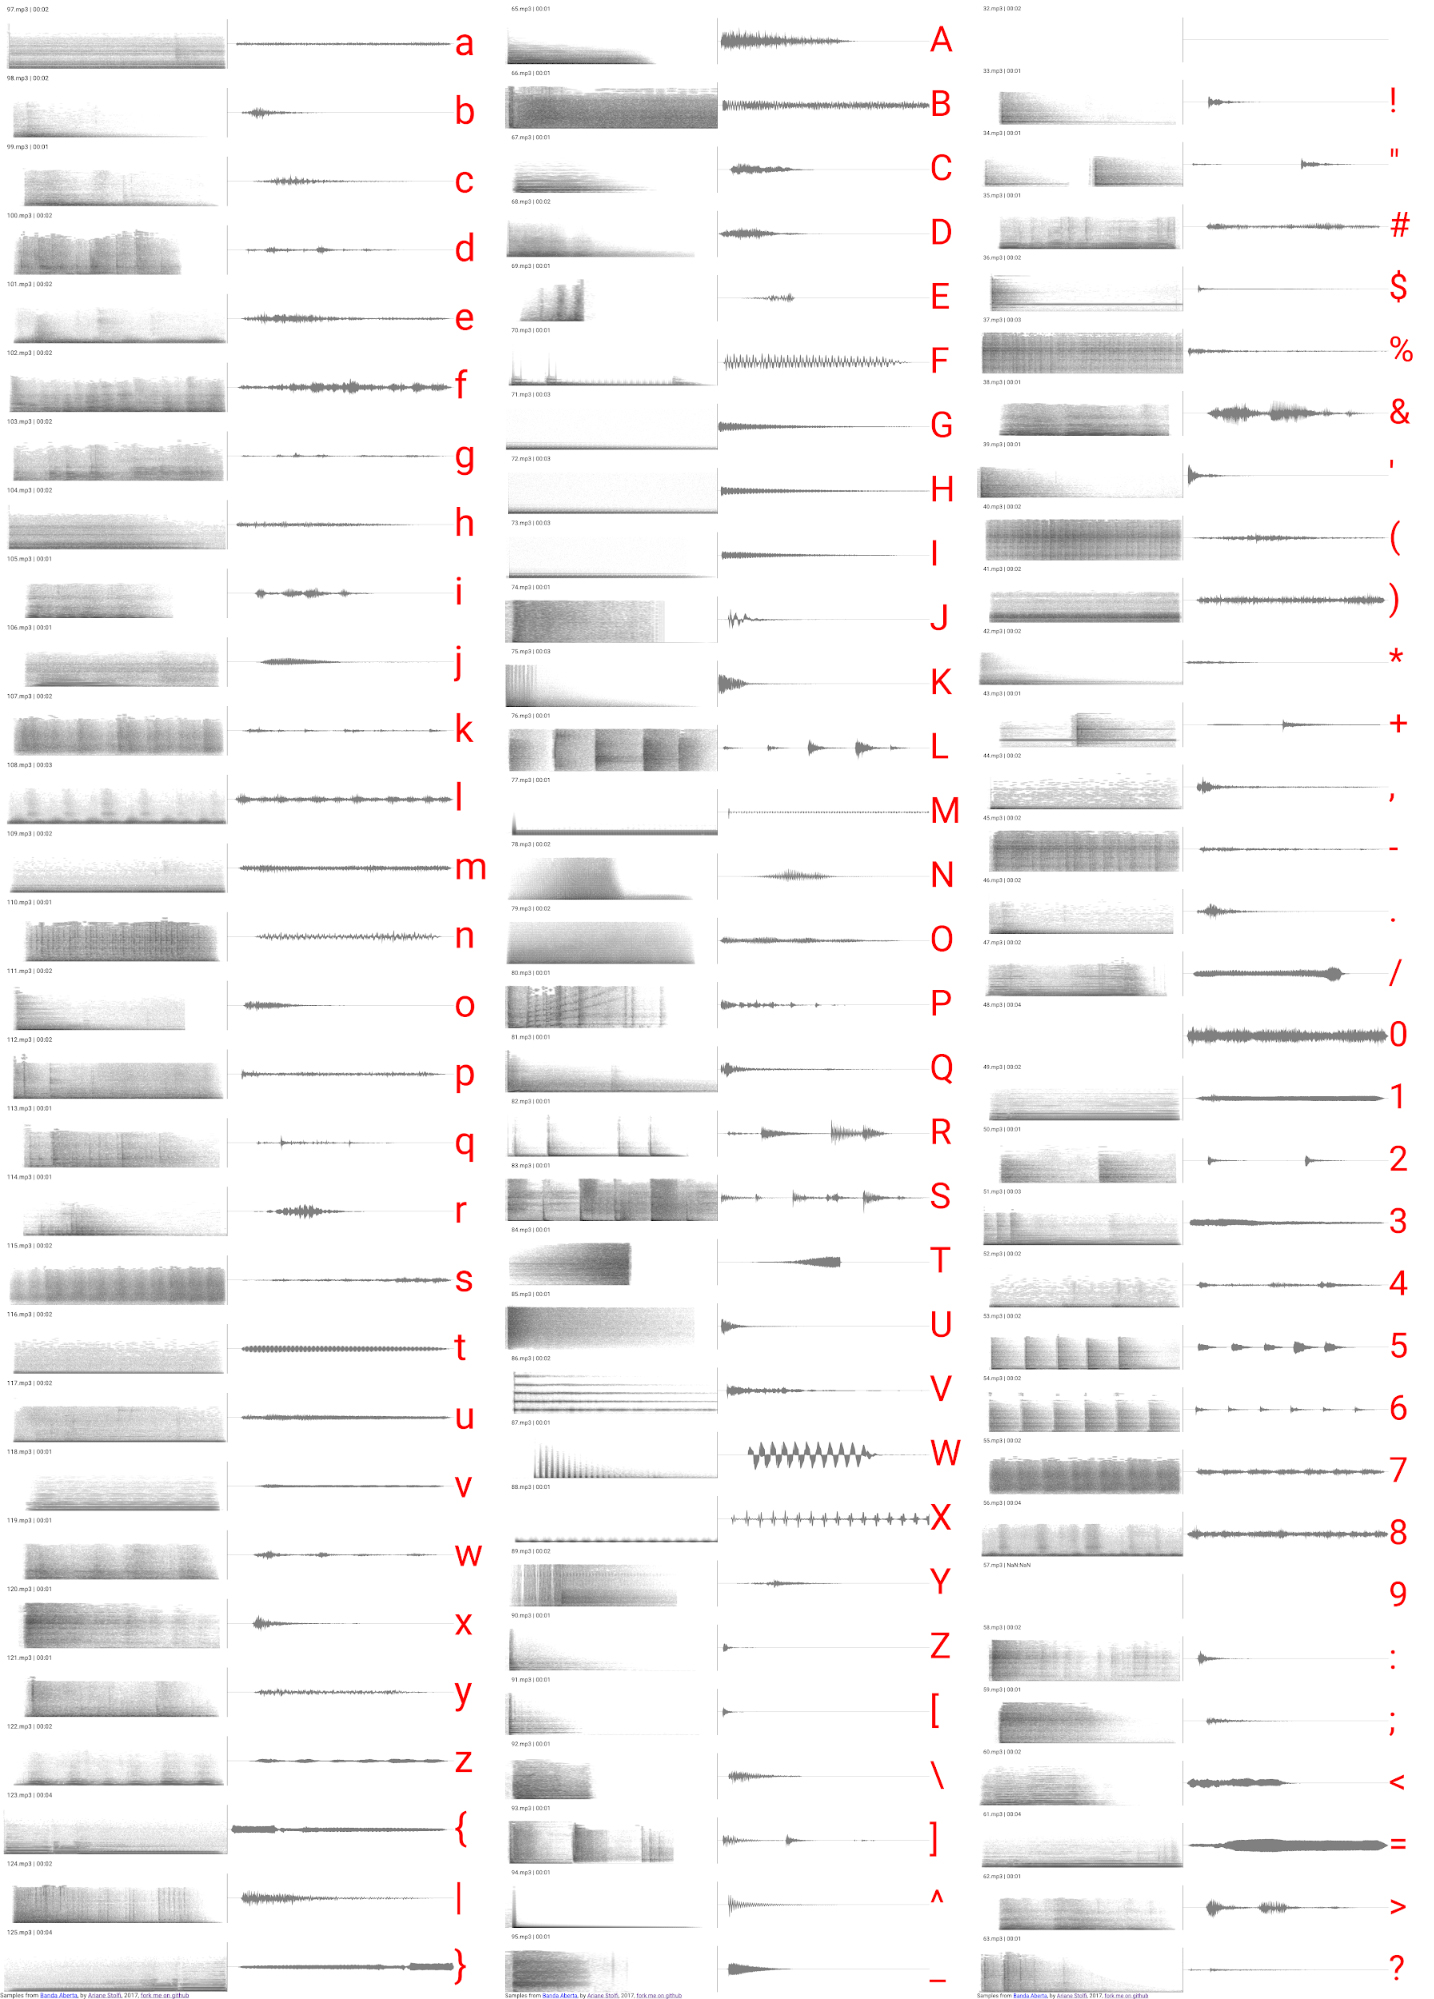
\includegraphics[width=0.7\linewidth]{pictures/cap3/bandaorquestra.jpg}
    \end{center}
    \legend{Fonte: screenshot da autora}
\end{figure}

%It is important to emphasize that the browser used by the participants can make a real difference on the performance itself. Most current browsers do enable web audio synthesis, however they are incompatible with many parameters. That said, the participants are recommended to use Google Chrome and take advantage of its full compatibility with current web audio standards.
\subsection{Segunda Versão: Web Audio Type -- Tipografia sonora}
Em uma segunda versão do projeto \cite{Stolfi2017w}, onde nosso objetivo era testar uma versão totalmente baseada em síntese sonora no browser, procuramos explorar uma abordagem diferente para o processo de tradução intersemiótica. Nesta segunda versão, desenvolvemos um sistema de analogia direta entre as formas das letras e o perfil espectral dos sons gerados, criando um ``alfabeto sonoro'' que ao mesmo tempo em que soava, desenhava a forma do texto no espectro. Para tanto, fizemos uma associação entre osciladores -- que desenhavam as linhas horizontais e as inclinadas -- e um sintetizador de rúido baseado em FFT que foi desenvolvido especialmente para o projeto -- que construía os blocos verticais das letras desse alfabeto sonoro.

Durante o desenvolvimento desta nova versão, nós optamos por avaliar a possibilidade de integração com algumas soluções pré programadas para síntese sonora via web, como os \emph{frameworks} Gibber \cite{Roberts2012gibberlivecoding}, Waax~\cite{Choi2013waax}, e meSpeak.js~\footnote{meSpeak.js website: \url{http://www.masswerk.at/mespeak/}}. Utilizar soluções prontas para síntese sonora poderia faciliar o uso e compatibilidade da tecnologia, mas ao mesmo tempo também criariam certas barreiras e imporiam algumas limitações que não são oferecidas pelo uso de web audio ``puro''. Além disso, algumas desses frameworks ofereciam muito ais recursos do que o necessário pelo projeto, que poderia dificultar o processo de desenvolvimento. Nós tentamos usar o framework meSpeak como uma ferramenta simples para conversão de texto em discurso, mas o resultado sonoro final não foi musicalmente satisfatório, e ele não permitia que se tocassem mensagens umas em cima das outras. No final, decidimos desenvolver uma solução toda em Web Audio, para a programação do processamento de áudio.



%During the development of this new version we opted to evaluate some ready-made solutions for web audio synthesis like Gibber~\cite{Roberts2012gibberlivecoding}, Waax~\cite{Choi2013waax}, and meSpeak.js~\footnote{meSpeak.js website: \url{http://www.masswerk.at/mespeak/}}.
%These solutions are able to facilitate the use of web audio technology and other browser facilities, but also create barriers and sometimes limitations that weren't imposed by pure web audio. Furthermore, sometimes frameworks could offer more than what was required by the application, which can lead to more confusion during development. We tried to use, meSpeak.js as a simple and interesting text-to-speech library but the resulting sound was not musically satisfactory, and we couldn't make messages play one on top of each other, due to limitations of the framework, so we choose to focus on pure web audio for sound programming.

Após as primeiras experiências com síntese de voz, decidimos por uma outra abordagem estética, baseadas em conceitos de design tipográfico \cite{ruder_typography:_2009} para propor uma ``tipografia sonora'', e também para experimentar com novas formas de fazer música, evitando acordes e escalas tradicionais da música ocidental. Essa idéia guiou toda a proposta de desenvolvimeto dessa nova versão e causou um grande impacto no resultado obtido.

Essa idéia de ``tipografia sonora'' já havia sido explorada em um trabalho anterior que eu desenvolvi em 2014, chamado ``Utopia'', onde trabalhei a com síntese subtrativa a partir de uma base ruidosa, que era a gravação de uma serra de fita em atividade, para desenhar a palavra UTOPIA no espectro sonoro. Nesse caso, bem como na versão em web audio do Banda Aberta, nós também partimos de uma idéia de tradução intersemiótica, assim como na outra versão, mas aqui, procuramos uma relação de isomorfia entre o desenho das letras e som, dispensando a relação fonética. Para tanto, projetamos ``letras'' formadas por blocos de sons pré-determinados, através de síntese aditiva e síntese de ruído, para sonificar o desenho das letras do alfabeto.



%We also decided to follow some aesthetic concepts based on type design~\cite{ruder_typography:_2009} to propose ``an audio typograph", and also to experiment with new kind of music, avoiding traditional chords and scales. These concepts surrounded the whole development of this current version of Open Band and had a great impact in the new result obtained.

%In this particular version, we are also using a concept of audio typography as base to this inter-semiotic translation, to decode letters into sounds, building spectral designed ``letters" made of predetermined sound blocks. Trough this path, we are abstracting the aural aspects of the typed characters and grabbing only the shape of the letters as information for the sound synthesis.

%The effect of typography on written texts acted as a motivation in the present artifact to experiment with ways in which timbre could affect the sound produced by musicians. We use additive and noise synthesis to sonify ``drawings" of the shapes of the letters.


\begin{figure}[!ht]
    \centering
        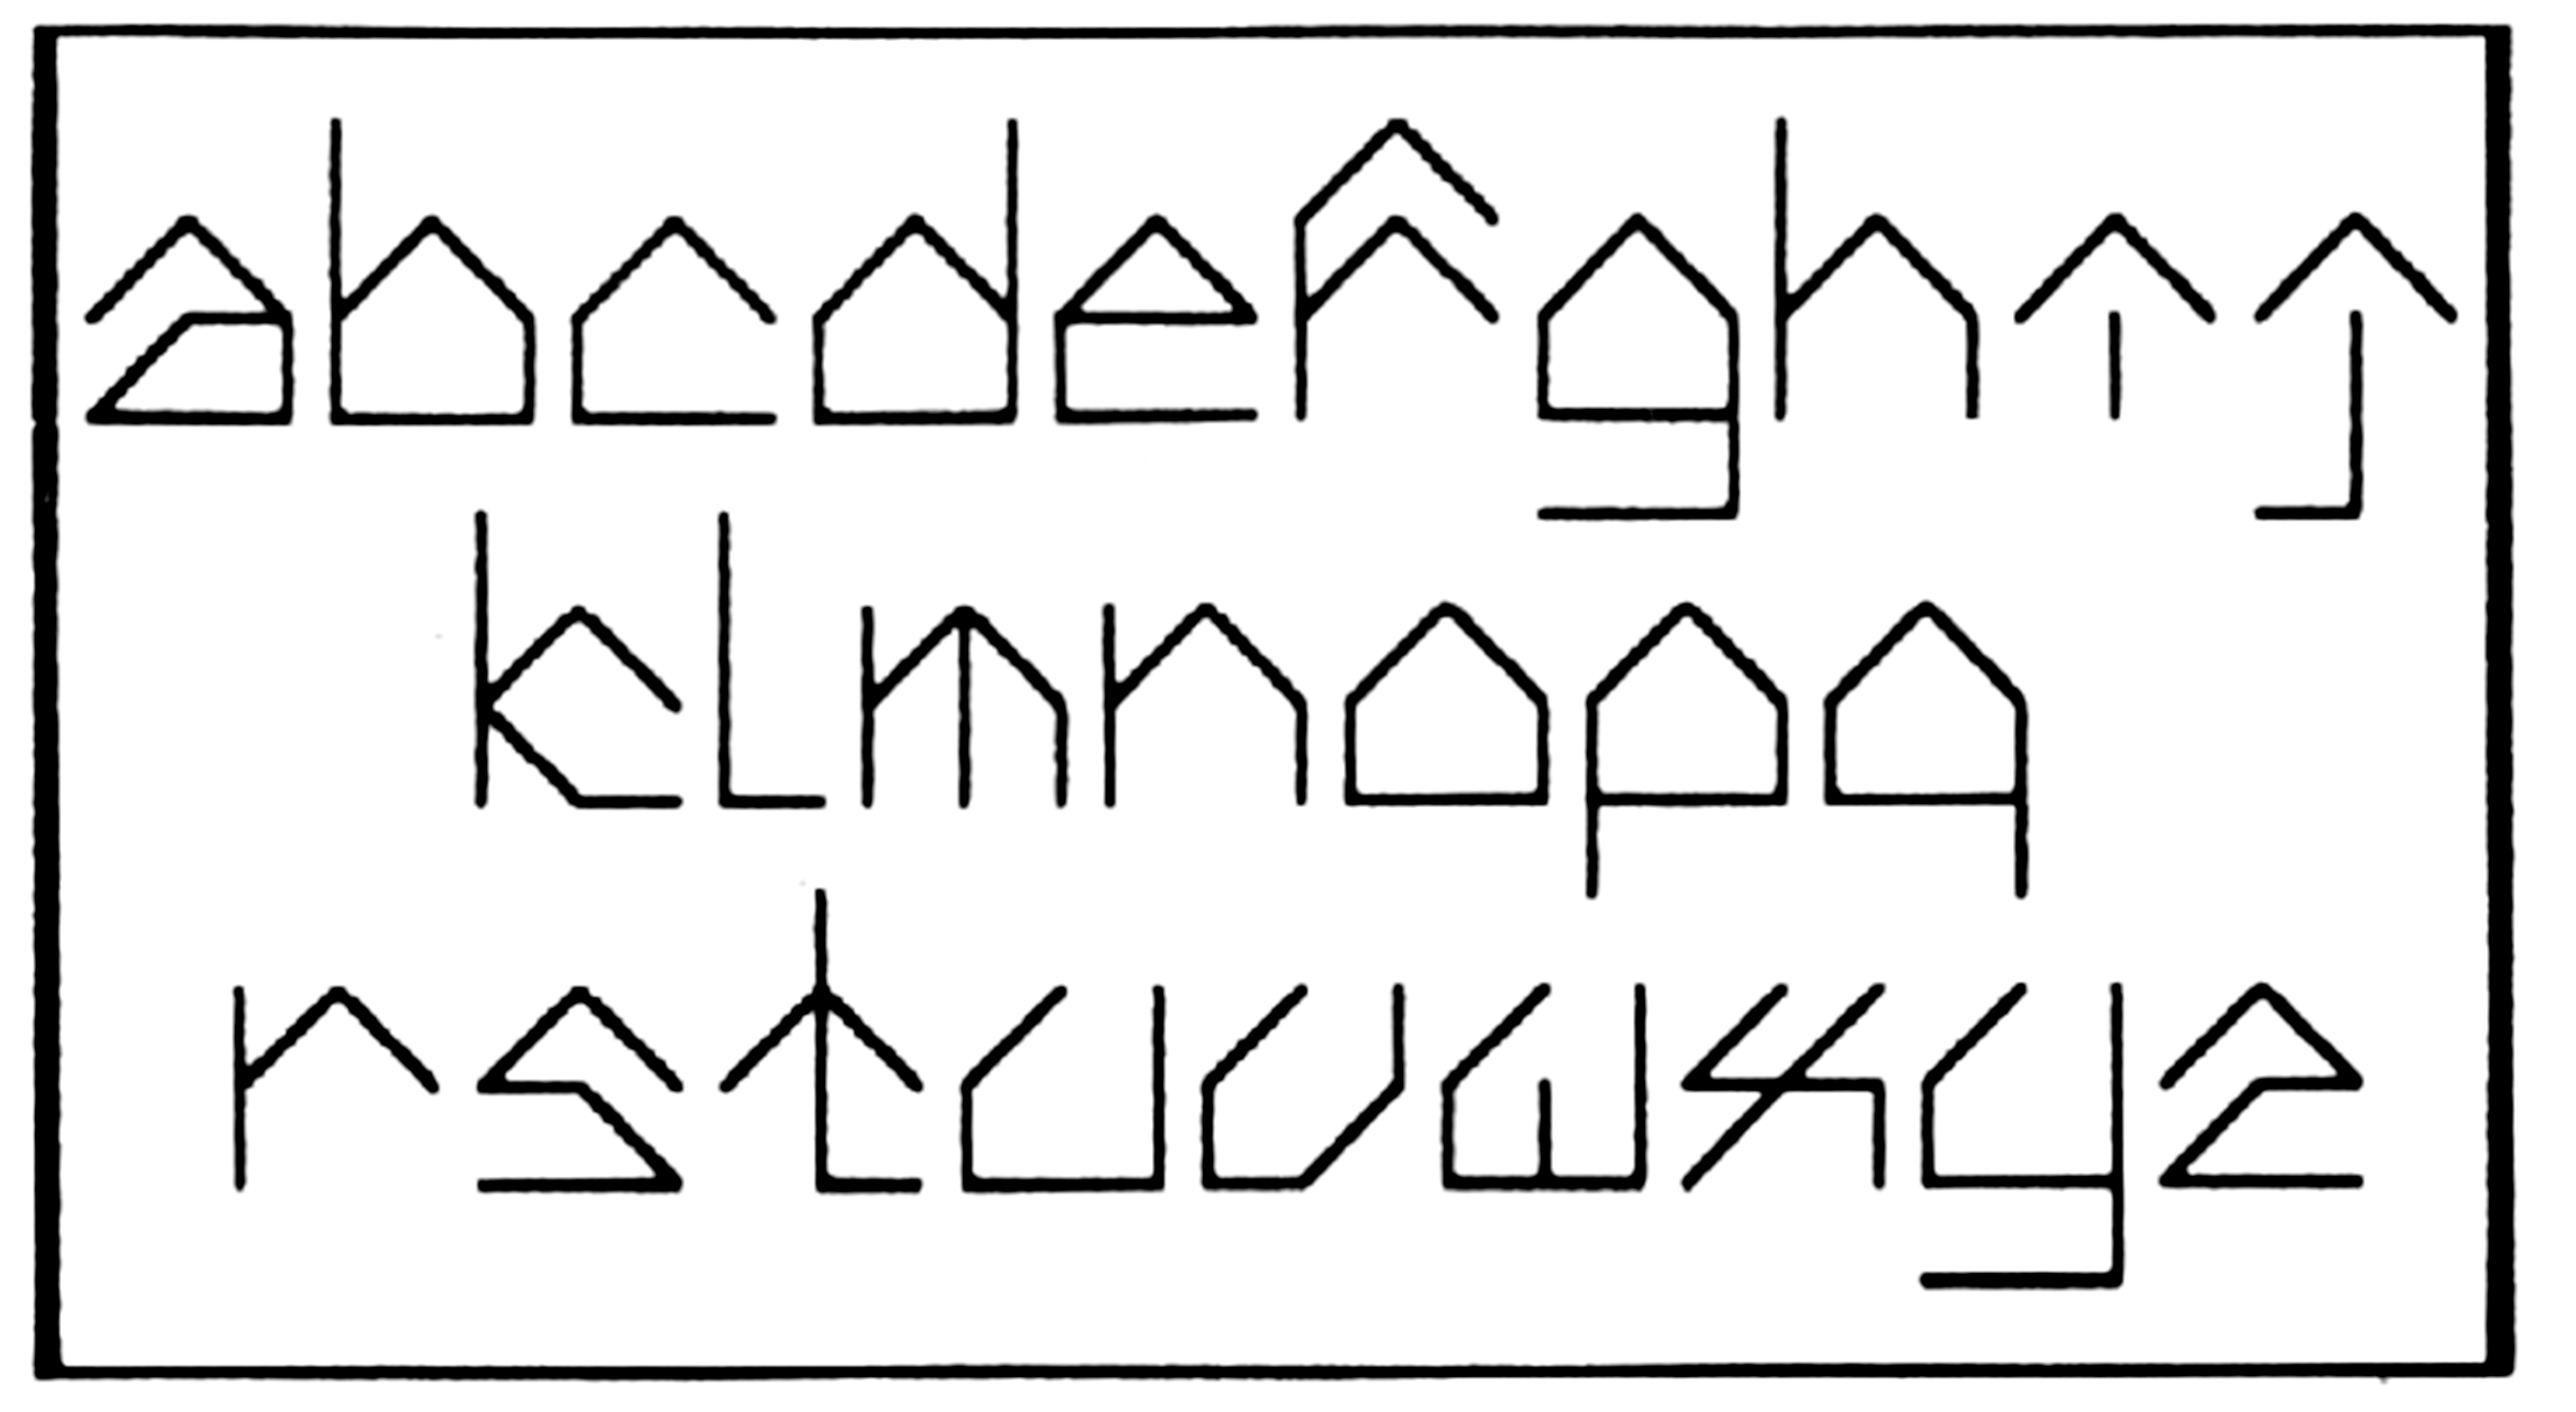
\includegraphics[width=0.8\linewidth]{pictures/metamagical}
        \vspace{-10pt}
    \caption{One of the modular alphabets proposed by Douglas Hoefstader in the book Metamagical Themas, page 90}
    \label{fig:metamagical}
\end{figure} 

Um dos pontos de partida para essa idéia foi o trabalho de Donald Knuth, um cientista da computação que trabalhou com questões de tipografia, e desenvolveu o conceito da ``meta-fonte'', um tipo que não era desenhado estaticamente, mas cujo desenho poderia variar de acordo com parâmetros tipográficos\cite{knuth-meta-font_1982}. A partir do design dessa ``meta-fonte'', muitas famílias tipográficas diferentes poderiam ser geradas, simplesmente pela mudança de parâmetros como: altura, largura, espessura, linha de base, altura de x etc. Como aponta Douglas Hesfstader:

\begin{citacao}
Knuth's purpose is not to give the ultimate parametrization of the letters of the alphabet (indeed, I suspect that he would be the first to laugh at the very notion), but to allow a user to make ``knobbed letters" -- we could call them letter schemas. This means that you can choose for yourself what the variable aspects of a letter are, and then, with Metafont's aid, you can easily construct knobs that allow those aspects to vary. 
(...)
Knuth's purpose is not to give the ultimate parametrization of the letters of the alphabet (indeed, I suspect that he would be the first to laugh at the very notion), but to allow a user to make ``knobbed letters" -- we could call them letter schemas. This means that you can choose for yourself what the variable aspects of a letter are, and then, with Metafont's aid, you can easily construct knobs that allow those aspects to vary~\cite{Metamagical1986}. 
\end{citacao}

%Donald Knuth, a computer scientist and artist who worked on typesetting issues, developed the concept of a ``meta-font", a typeface that was not statically drawn, but that could be changed trough typographical parameters\cite{knuth-meta-font_1982}. Following the rules of meta-fonts, many different typefaces could be generated simply by varying the type parameters. As says Douglas Hoefstader in ~\cite{Metamagical1986}, \textit{``Knuth's purpose is not to give the ultimate parametrization of the letters of the alphabet (indeed, I suspect that he would be the first to laugh at the very notion), but to allow a user to make ``knobbed letters" -- we could call them letter schemas. This means that you can choose for yourself what the variable aspects of a letter are, and then, with Metafont's aid, you can easily construct knobs that allow those aspects to vary."}.





\begin{figure}[!ht]
   \centering
       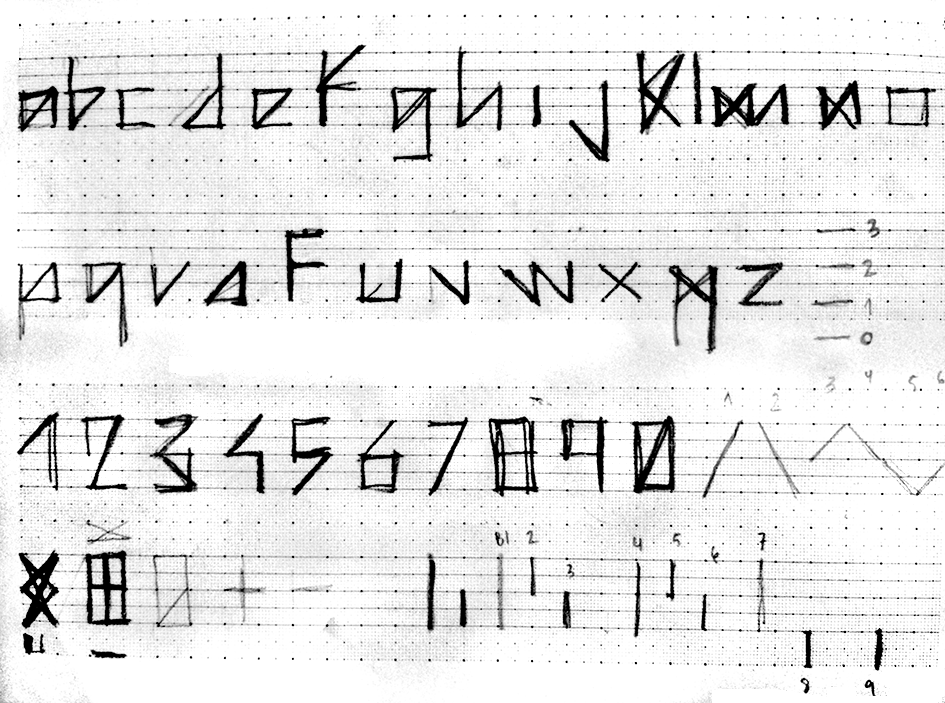
\includegraphics[width=0.8\linewidth]{pictures/audiotype_sketch}
   \caption{Sketch for the modular font to be base for audio synthesis.}
    \label{fig:sketch}
 \end{figure}


%\begin{figure}[!hb]
%   \centering
%       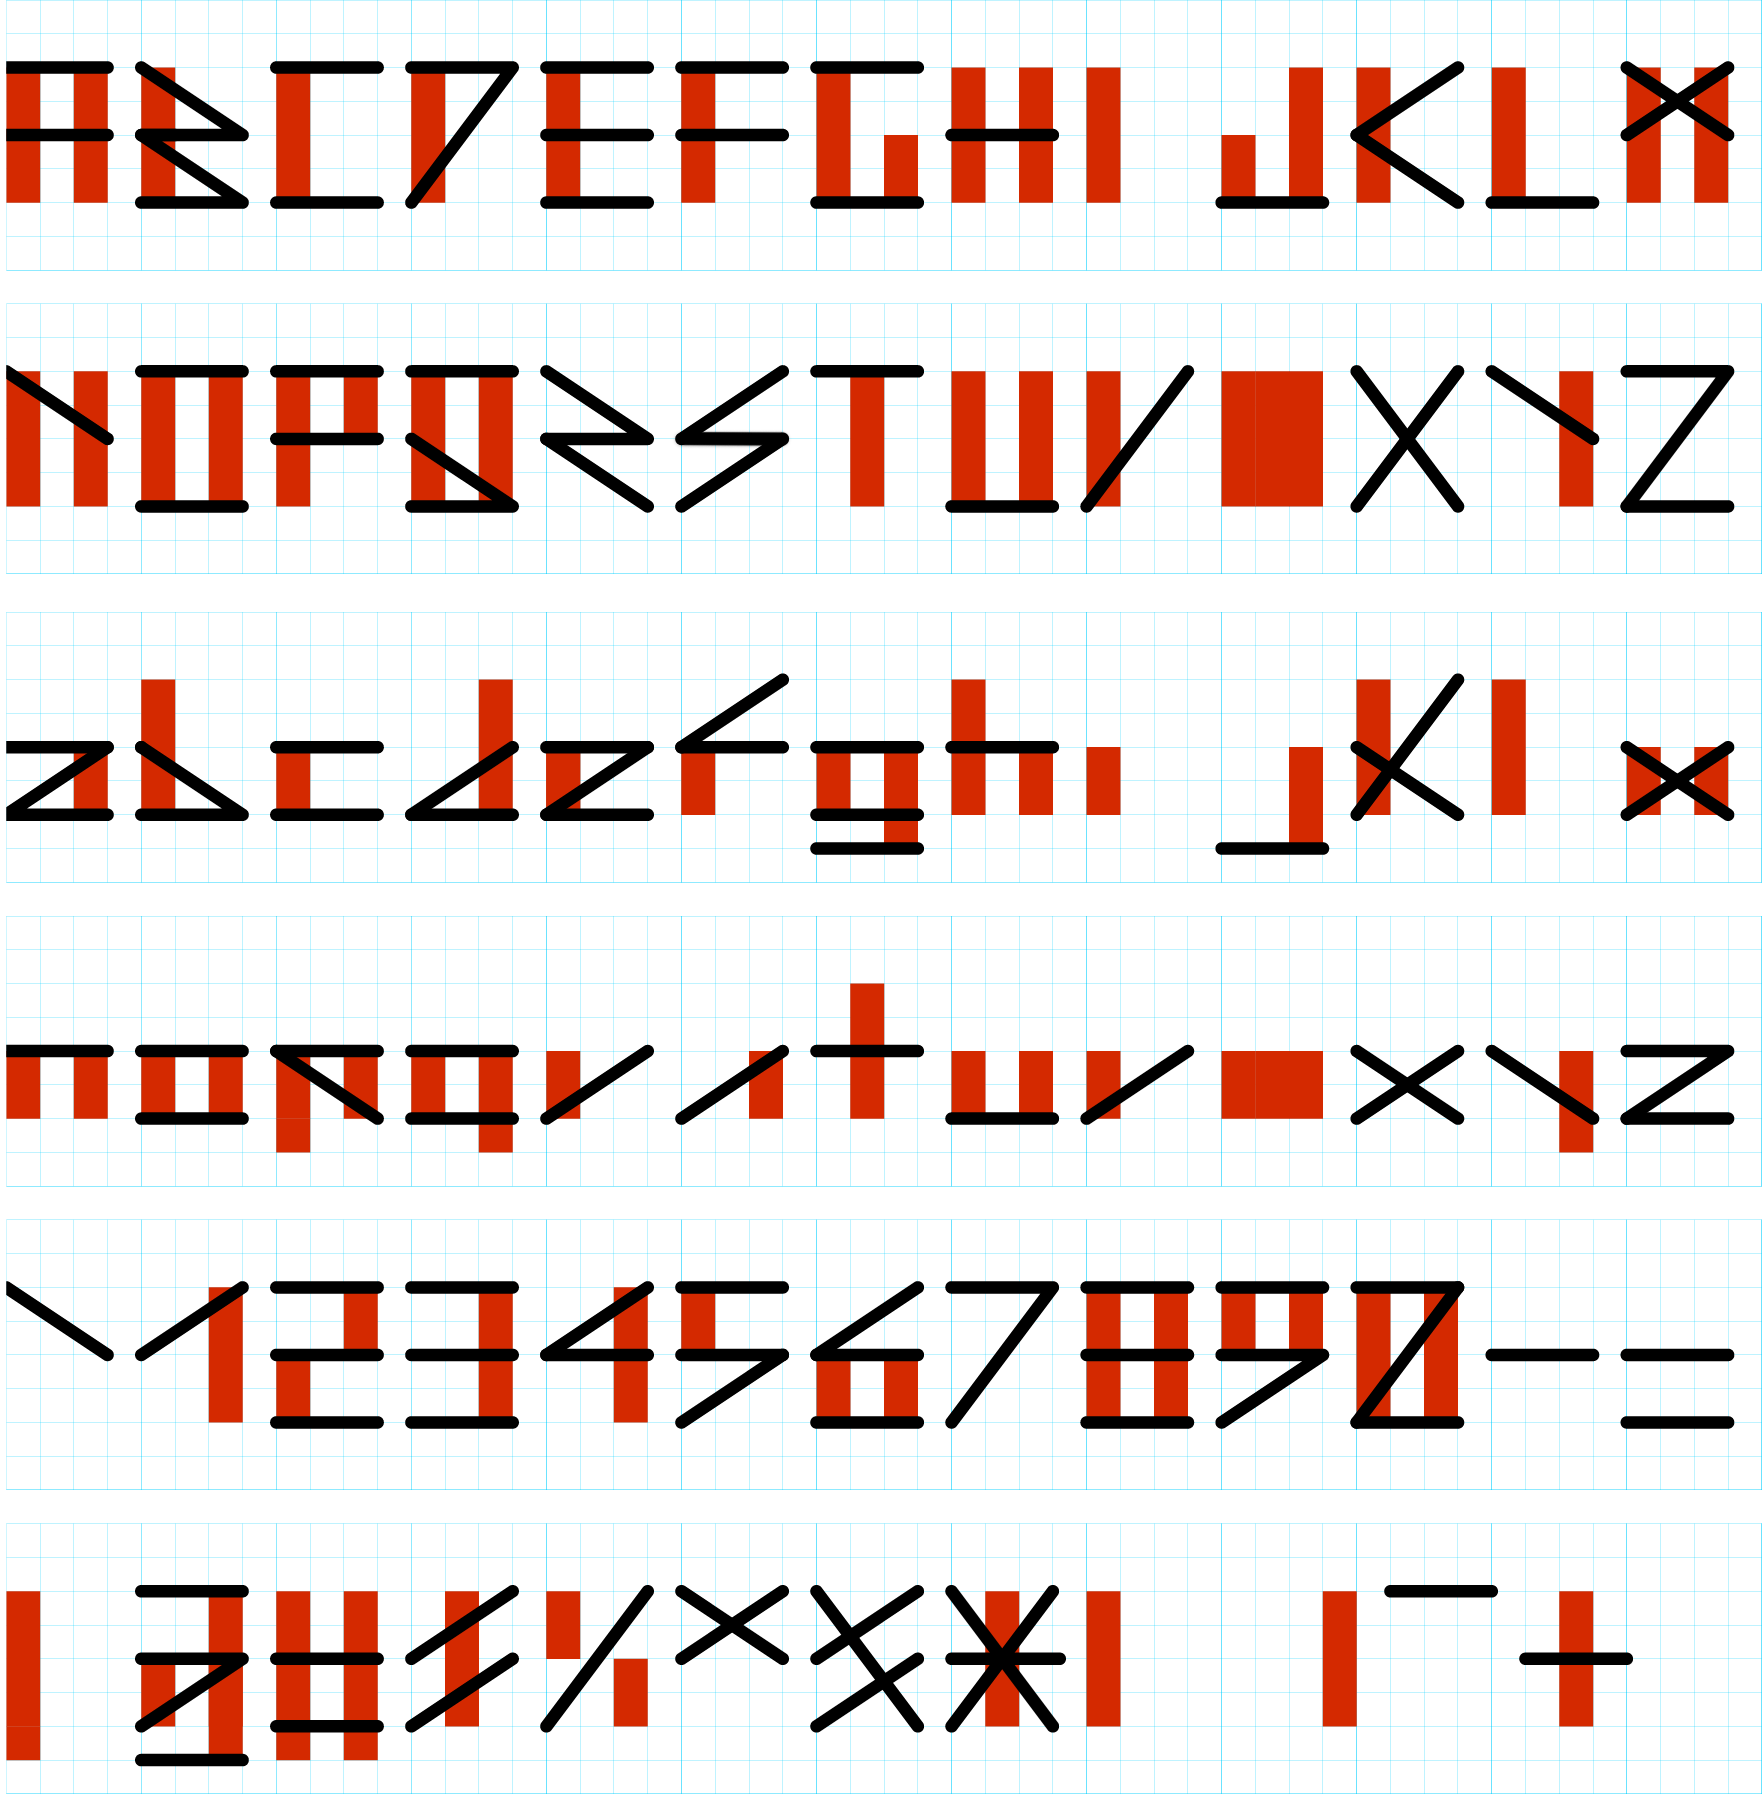
\includegraphics[width=0.45\textwidth]{pictures/audiotype_v1_2_2}
%       \vspace{-10pt}
%   \caption{Project for audio typography, made of blocks of noise, sine waves and glissandi. The red blocks represent noise and the black lines solenoids and glissandi.}
%   \vspace{-10pt}
 %   \label{fig:project}
%\end{figure}

Nós usamos alguns desses parâmetros tipográficos definidos por Knuth para estabelecer frequências geradoras para os sons puros: as frquências mais baixas corresponderiam às linhas dos descendentes, a linha de base para a segunda, a altura de x para a terceira e a altura da caixa para a quarta frequência, em ordem ascendente. Os parâmetros horizontais, por sua vez, foram convertidos em medidas temporais, para determinar a duração dos eventos sonoros e dos intervalos entre as letras.

%We used the basic parameters defined by Knuth~\cite{Metamagical1986} such as x-height, baseline, height of ascendants and descendants, as measures to establish frequencies for tone sounds (one low, one at the baseline, one at the x-height an one at the uppercase line of each letter). The horizontal parameters of the type are translated into temporal measures, to determine duration of the sound events and intervals between the letters.   

A meta-font proposta por Knuth é uma fonte complexa com cerca de 36 parâmetros tipográficos variáveis. Para a nossa ``tipografia sonora'', no tentanto, propus uma analogia mais simples, semelhante às propostas por Douglas Hoefstader no seu livro ``Metamagical Themas''\cite{Metamagical1986}(ver Figura \ref{fig:metamagical}), baseada em uma estrutura de grelha. Na nossa proposta, as letras seriam desenhadas a partir de poucos elementos básicos, como no rascunho apresentado na figura \ref{fig:sketch}. As linhas das letras foram mapeadas em dois tipos de funções: síntese de noise (noise())baseada em FFT para os blocos verticais, e senóides (sine()) para as linhas horintoais e diagonais (que soam como glissandos), como pode ser visto nas Figuras \ref{fig:noise} e \ref{fig:sine}. 


%A meta-font is a complex font with several typographic parameters. In this work, we are using a simpler analogy by proposing a modular type, similar to the ones Douglas Hoefstader~\cite{Metamagical1986} proposes in his book ``Metamagical Themas", based on simple grid structures (see Figure \ref{fig:metamagical}). We propose a model that can work only with a few building blocks (see Figure in which they are sketched). The line of the letters was mapped into two basic types of functions: noise synthesis for the verticals and solenoids for the horizontal lines and glissandi, as defined by the composer project in Figure x.


A função ``sine()'' tem um \emph{buffer} de oscilador e podem gerar frequências estáticas ou em rampas lineares, deste modo, geram linhas horizontais ou diagonais no spectro. As funções ``noise()'' geram blocos de ruído que vão de faixas de frequencia determinadas. Como processo de programação, definimos 20 funções específicas para cada módulo das letras e cada letra é então formada pelos seus módulos correspondentes. 





%Sine function has one oscillator buffer that can have static frequencies or linearly ramping frequencies. This creates diagonal and horizontal lines in the spectrum. Then, frequencies are defined as the bottom and top limit, some steps are defined in the middle. The length of spectral letters are as well defined. By the end, letters are translated as a group of functions, and the result is played one after another. We built 20 predetermined functions to correspond at each ``type block", and each letter plays as many functions as are determined by the typeface project. Thus, we created a system of mapping letters to the functions.

Cada nó de saída de audio passa também por um envelope ADSR \cite{Lee2016} para gerar uma forma mais natural de ataque e release, e também passa por um nó de ganho que pode ser controlado durante a performance. A figura \ref{fig:spectro}, mostra um espectrograma gerado pelo sistema com os resultados obtidos.

%Every output node goes through an ADSR class \cite{Lee2016} that creates a more natural attack/release, and also goes through a gain node, that can be changed during a performance. On Figure \ref{fig:spectro} is shown a spectrogram generated by the application with the results obtained.

\begin{figure}[!ht]
    \centering
        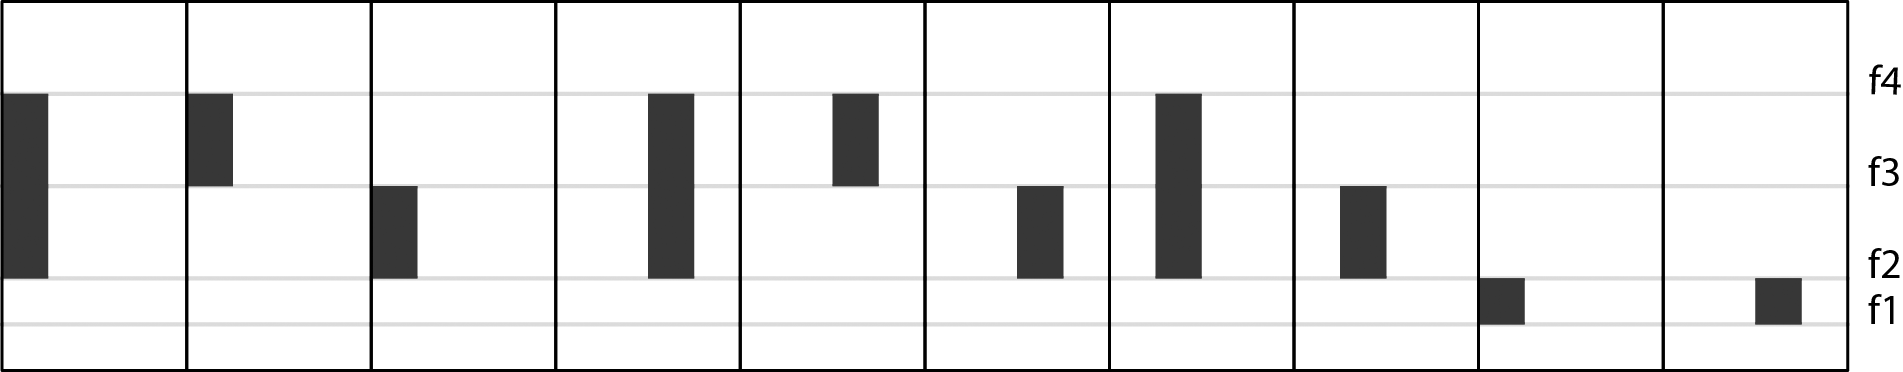
\includegraphics[width=1\textwidth]{pictures/audiotype_v1_noise}
        \vspace{-10pt}
    \caption{Functions for playing vertical blocks with noise synthesis}
    \vspace{10pt}
    \label{fig:noise}
        \centering
        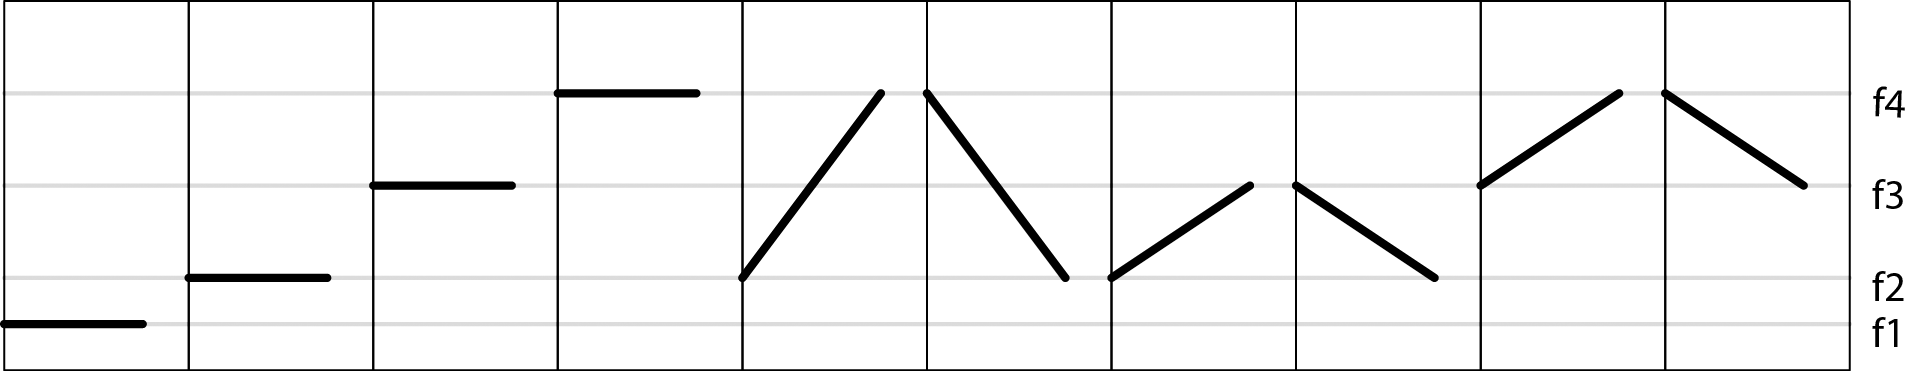
\includegraphics[width=1\textwidth]{pictures/audiotype_v1_sine}
    \caption{Functions for playing horizontal and diagonal lines with oscillators}
    \vspace{-10pt}
    \label{fig:sine}
\vspace{10pt}
\end{figure}

\begin{figure}[!ht]
    \centering
        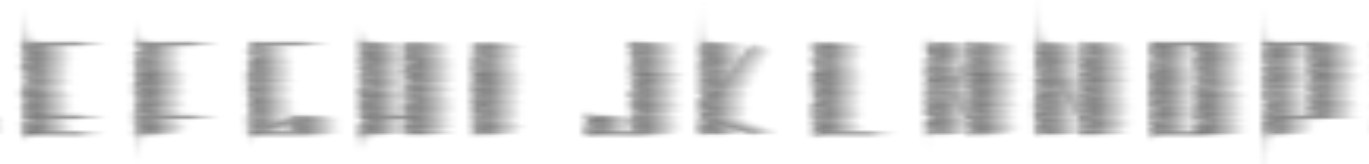
\includegraphics[width=1\textwidth]{pictures/spectrogram}
        \vspace{-10pt}
    \caption{Spectrograms generated by the application}
    \vspace{-10pt}
    \label{fig:spectro}
\end{figure}

%As every letter from every message is translated into a group of playing Web Audio nodes, the number of oscillators that plays simultaneously can grow really quickly depending on the number of participants sending messages. As this application was intended to play in many different mobile devices, this led to the necessity of limiting the creation of nodes, as this could take more processing than some devices could take, and in some cases could make the device stop playing, which is undesirable behavior for such application.






\subsection{Apresentações públicas}
Nós apresentamos o Banda aberta em diferentes ocasiões, para diferentes perfis de público. Dependendo do perfil dos participantes, a conversa foi para direções diferentes. Em uma primeira fase, apresentamos o projeto rodando em um servidor local, que era acessado através do endereço IP, para reduzir a latência e manter o público reunido em uma mesma rede. Posteriormente, passamos a usar a versão online do sistema em outras performances, para facilitar o processo de montagem. Até o momento, realizamos as performance seguintes:

\begin{description}

\item[Ensaio no Nusom] 
A primeira apresentação informal do projeto aconteceu na reunião do NuSom do dia 9 de maio de 2016. O público presente era de pesquisadores do grupo, e cerca de 9 pessoas participaram da experiência. Notamos uma diferença considerável de tocabilidade entre quem estava com laptop em relação a quem estava com celulares. O site também não funcionava em todos celulares, especialmente modelos de iphone mais antigos. \footnote{Registro da apresentação em \url{https://www.youtube.com/watch?v=Utc_4mT5b8s}}

\item[Festival Bigorna]
No dia 26 de junho de 2016, estreamos publicamente o projeto no Festival Bigorna, que aconteceu na Praça José Molina, próxima à Avenida Paulista em São Paulo. O Estúdio Fita Crepe, um pequeno espaço dedicado à produção e difusão de música experimental organizou o festival que ocupava essa praça considerada subutilizada, pela sua localização\footnote{A programação do festival está disponível em: \url{http://www.festivalbigorna.com/2016/}}.

\begin{figure}[!ht]
	\centering
		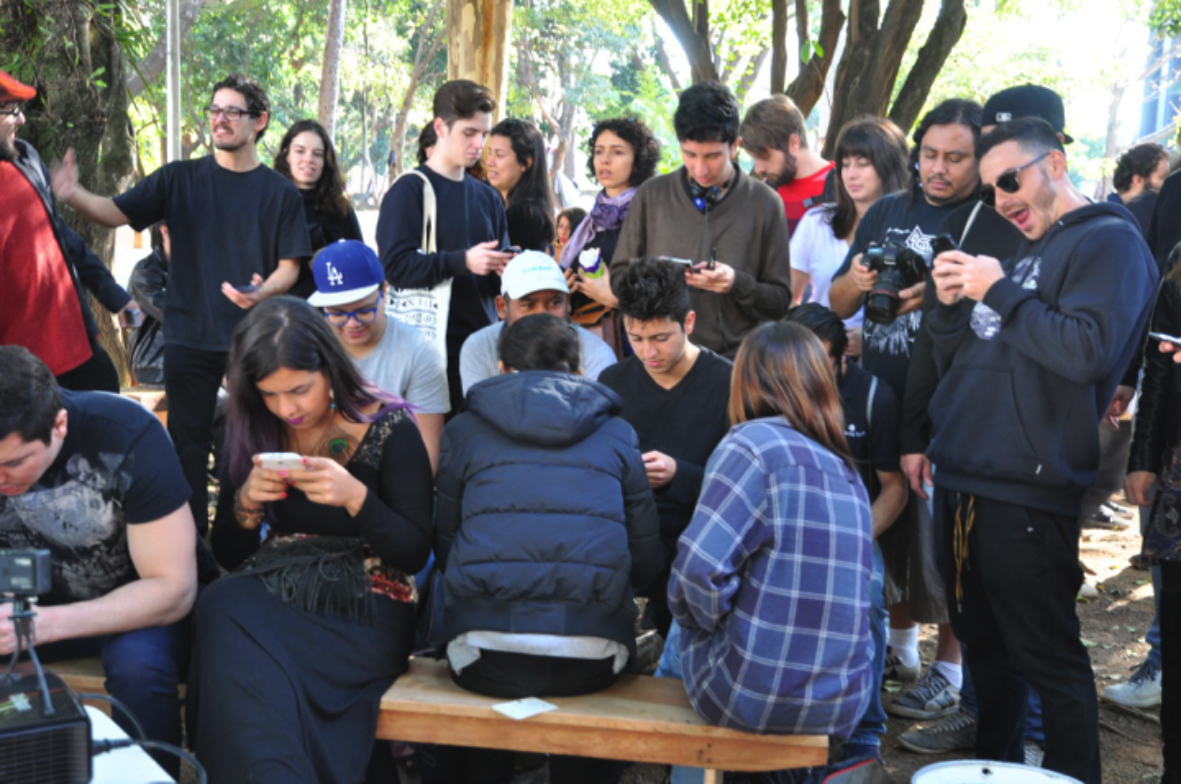
\includegraphics[width=1\textwidth]{pictures/bigorna}
		\vspace{-10pt}
	\caption{people interacting within the piece}
    \label{fig:performer}
\end{figure}

O público presente no momento era de cerca de 80 pessoas, mais do que o roteador podia comportar (30 pessoas ao mesmo tempo), o que deixou várias pessoas de fora da interação. A audiência incluía membros do NuSom, músicos da cena experimental e o público geral do festival, mas grande parte era formada pelos estudantes de produção musical que colaboraram com o terceiro conjunto de samples. Jovens, ficaram bastante eufóricos com a possibilidade do anonimato e praticaram um certo nível de \emph{bulling} entre eles. 

\item[Rádio grave] 30 - 6 -2016
Fomos fazer uma performance também na Rádio Grave, uma rádio web que foi montada no Gfau para ajudar na mobilização dos  estudantes durante a greve do ano passado. Os locutores simulavam a ráfio era uma nave espacial, e a ``aterrisagem'' do Banda Aberta por lá rendeu um episódio que ficou conhecido como ``reset do universo'', pela surpresa gerada pelos sons fora do comum. Uma gravação do áudio da performance pode ser ouvido no seguinte link: https://soundcloud.com/asss/banda-aberta-na-radiograve-reset-do-universo.


\item[¿Musica? 12]
No festival, que faz parte de uma série organizada pelo NuSom, apresentamos pela primeira vez a segunda versão do projeto, com síntese sonora em Web Audio, para um público formado principalmente por alunos e professores da Música. 
\url{https://www.youtube.com/watch?v=hRELFhQm6M0&t=639s}


\item[Web Audio Conference] 


\item[Female Laptop Orchestra]
Na performance ``Trasnmusiking'', realizada pelo grupo Female Laptop Orchestra, utilizamos o projeto Banda Aberta em uma apresentação realizada em Londres durante a conferência ``Audio Mostly'' de 2017. A peça contou com a participação remota de 12 pessas, que mandavam streams de áudio de lugares diferentes do globo, esses streams eram mixados em tempo real por Anna Xambó. Além disso, utilizávamos o Banda aberta em uma versão com síntese por web audio, mas somente de ruído, para receber feedback em tempo real da audiência, e também performei com técnicas vocais estendidas e percussão. A audiência era formada principalmente por participantes da conferência, em sua maioria acadêmicos da área de tecnologia musical. A audiência utilizou o chat para dar opiniões sobre a performance e também para piadas com membros da equipe, pricipalmente Alo, que era um dos organizadores da parte musical.


\item[Audio Mostly Workshop]
Durante o workshop Sounds in the Cloud, organizado em um trabalho conjunto pela equipe do projeto Audio Commons da Queen Mary University of Londo e pela equipe de pesquisadores do sistema de \emph{Machine Learning} RapidMix da Universidade Golsdmith, os participantes foram convidados a explorar ferramentas desenvolvidas pelos pesquisadores em grupos. Nossa equipe desenvolveu uma versão do projeto Banda Aberta que utilizava a ferramenta RapidMix para mudar parâmetros sonoros através da captura de movimentos pela câmera. Com isso, era prossível treinar o sistema para reconhecer certos movimentos em tempo real. Com a experiência, foi possível verificar tanto a facilidade de adaptação do nosso sistema para incorporar tecnologias ded terceiros, quanto a facilidade de utilização do sistema RapidMix para ser incorporado em demais projetos de interação através de sua API em JavaScript.

\item[Encontro da rede de Tecnoxamanismo] 12-8-2016
O encontro da Rede de Tecnoxamanismo na Dinamarca aconteceu na cidade de Aarhus, no ``Dome of visions'', um domo geodésico na região portuária da cidade, onde acontecem uma série de eventos ligados à sustentabilidade, agroecologia, ecologia e temas afins. Além de colaborar na produção do Evento, apresentei a performance para um público que incuía músicos, produtores, performers e interessados de uma maneira geral. O público foi muito comportado no sentido de não escrever muitas bobagens no chat. Nesta performance, utilizamos a versão online da ferramenta, sem o servidor local.


\item[SHA Festival] 7-8-2017
O Festival ``Still Hacking Anyway'' é um encontro de hacker, programadores, pensadores e ativistas que acontece de quatro em quatro anos na Europa. Na edição de 2017 do evento, apresentamos o projeto em uma performance de 45 minutos, onde participaram interessados de diversas partes do mundo. Por ser um festival hacker, a maior parte do público portava laptops ao invés de celulares, o que permitiu uma maior agilidade na digitação das mensagens. Alguns dos presentes passaram a performance tentando hackear com o intuito de derrubar o sistema, o que ocorreu a cerca de 40 minutos depois do início, através de um script que sobrecarregava o sistema e causou uma pane no audio buffer. Pelas características do evento, já esperávamos um comportamento deste tipo por parte da audiência, que ocorreu até mais devagar do que o esperado. O ataque, no entanto, não causou nenhum tipo de dano ao servidor, que voltou ao normal logo que a performance se encerrou.

\item[aMostra Sonora] 2-7-2016
Na apresentação que fiz solo no festival aMostra Sonora em 2016, utilizei um patch de Pure Data que venho desenvolvendo desde 2006, chamado modulari, que se baseia em samplers, sintetizadores por \emph{waveshaping}, efeitos para o microfone e osciladores, em conjundo com o Banda aberta. Durante a performance, que durou 40 minutos, utilizei os dois sistemas e técnicas vocais expandidas em conjunto. Apesar de ter corrido normalmente, considerei que os resultados sonoros do conjunto ainda eram limitados, na possibiliade de variação sonora, e passei a planejar um sistema alternativo que fosse mais rico também para performances solo, que descreverei na próxima seção desta tese.




\item[Congresso da Abrapem]

No congresso da Associação Brasileira de Performance musical (30 de junho de 2016), o público de cerca de 23 pessoas, era majoritariamente formado por músicos tradicionais, que ficaram perguntando sobre as referências musicais, de onde vieram os samples, e experiemntaram bastante com possibilidades rítmicas. Um registro da performance pode ser visto em:  \url{https://www.youtube.com/watch?v=NOWapLq6eiU}.



\item[Concerto de Computação Musical no IME] (22-9-2016)
No concerto de computação musical no IME aconteceu uma coisa inusitada, o público era formado majoritariamente por programadores e um dos participantes percebeu que era possível inserir comandos em HTML e CSS através do chat. Logo, os participantes começaram a encher a tela com formas geométricas e letras em movimento, e ficaram eufóricos com essa possibilidades de hackear o chat. A gravação da tela da apresentação pode ser vista em: https://www.youtube.com/watch?v=xs23z1IfPfY. A facilidade de uso levou a um grande engajamento do público durante as performances, e traz também um grande nível de divertimento, aproximando assim, como desejávamos, atividade musical de um contexto mais lúdico como o de jogo.

\item[Áudio Insurgência] (7-10-2016)

No festival Áudio insurgência (8 de outubro de 2016), o público era formado principalmente por membros e entusiastas da cena de música experimental e noise de São Paulo. A mesa de som da casa estava com defeito, então ligamos ligamos o celular diretamente nas caixas de som. Também não havia projeção, então não se estabeleceu um ponto focal, e as pessoas ocuparam todos os espaços da casa com seus dispositivos. A gravação do chat pode ser vista em: https://www.youtube.com/watch?v=DpCuU41tWM8 

\end{description}







\section{Análise preliminar}

%comment: In section 4, the authors allude to issues of cross-browser compatibility, but in 3.3.8 they suggest it "is working correctly" on all major browsers. This seeming contradiction needs to be resolved, and hopefully in a way that explains in more detail the issues encountered, the solutions, and any broader take-aways in terms of the future of web audio API.

Em uma análise inicial, foi perceptível que em contextos onde a audiência tinha mais relação com o meio musical, havia uma tendência maior dos participates passarem mais tempo experimentando com os sons e com o ritmo, digitando mensagens sem significado discursivo. Quando o público era mais jovem, os participantes tendiam a jogar mais com a possibilidade de escrever anonimamente. Quando as conversações começavam a esquentas, camadas de sons eram sobrepostas, tornando o ritmo mais frentético.

Como em uma conversa real, se as pessoas não param para ouvir uns aos outros, a comunicação se torna mais confusa. Nós recbemos atrav´s do chat, durante as performances, uma boa quantidade de \emph{feedback} dos usuários, com pessoas perguntando tanto sobre o sistema quanto sobre os sons, e elogiando a performance.

%We observed that in musical contexts, the audience keeps more time experiencing with the samples and rhythm, typing meaningless phrases, and when the public is younger, the participants tend to play with the ability to speak anonymously. 
%As the conversation ``warms" up, layers of sounds are overlapped, turning the rhythm into something more frenetic. 

%Like in a real conversation, if people don't take time to listen to the others, the sound becomes more difficult to distinguish. We received a lot of feedback from the public on the chat, with people asking things about the project and supporting it.

Um problema da primeira versão do projeto era de que ela era baseada em um volume grande de dados dos samples (cerca de 60 mB), então era necessário criar uma rede local, pelo menos no Brasil, onde a qualidade das redes de internet é menor, e mesmo assim o sistema ainda demorava significativamente para carregar. Na segunda versão do projeto, que era baseada em síntese, o volume de dados foi reduzido dramaticamente, para apelas alguns kilobytes, o que reduziu também o tempo de carregamento do sistema. O uso de dados durante a performance, no entanto é baixo em ambas versões, uma vez que não há transmissão de áudio entre os usuários, somente de mensagens de texto, que em geral não são muito pesadas. 

%One problem of the previous version was that been based on heavy volume of data from samples, we had always to create a local network and even with that we had a long time of download before playing. With the present version relying only on web audio synthesis, the size of the project reduced dramatically --- from 60 megabytes to kilobytes --- and also the downloading time when compared with the previous version.
%This new aspect of the Open Band facilitates users to participate using 4G data plan as the data consumption is now comprised of text messages only as no samples files are downloaded. 

É importante emfatizar que o navegador utilizado pelos participantes pode causar uma diferença real durante as performances. A maioria dos navegadores atuais já suporta a webAudio API, mas alguns ainda são incompatíveis com certos parâmetros. Por este motivo, recomendamos a utilização do navegador Google Chrome, que é atualmente o mais compatível com os padrões definidos pelo W3C \footnote{W3C é a organização que define os padrões para as linguagens base da web, como HTML, CSS, JavaScript etc.}


%


\subsection{Análise da interação com a audiência}
%As described before, one of the design aims of the project is to facilitate participatory musical experiences for audiences who don't necessarily have a musical background. We aim to engage participants in situated playful interactions. In this Section we first describe the Open Band performances and then present our evaluation methodology.

Seguida a uma análise preliminar, procuramos fazer uma análise mais sistemática de algumas das performances apresentadas. Se olharmos para o projeto da perspectiva de um trabalho artístistico, nós procuramos analisá-lo como ``uma prática participativa, culturalmente posicinada em sem regras e gradações explícitas''\cite{McCullough1998}, ao invés de procurar analisar o projeto em termos de usabilidade, que seria um critário mais adequado a produtos de design. No entanto, nós procuramos buscar evidências de apreciação e engajamento. Uma das formas possíveis de se analisar segundo esses critérios foi analizando os registros de dados das mensagens enviadas durante as performances apresentadas ao público. Pensando no projeto como um aparato de comunicação, nós estávamos interessados em investigar a natureza dessas interações multi-usuários que aconteceram atráves do sistema de chat em alguns dos contextos dados. Para isso, procuramos investigar padrões linguísticos, para verificar como e se eles se relacionariam também como interações sonoras.


%When looking at the project from the perspective of an artwork, we are interested in analysing it as ``a participatory practice, culturally positioned, and without explicit rules or grading" \cite{McCullough1998}, rather than in terms of usability, a dimension more adapted to product design. We however also aspire to search for evidence of appreciation and engagement which have to do with usability, to an extent. One of the access points to study how people engaged in the Open Band performances is to analyse data logs of the messages that were sent during interactions. As a communication device, we are interested in the nature of the multi-user interactions occurring through the chat system in given contexts. We namely want to investigate linguistic patterns and if and how they are inter-related to specific audio interactions.

Para essa análise mais detalhada, contamos com o auxílio de um pós graduando em Ciência da Computação, Janis Sokolovskis, além do superfvisor do meu estágio na Queen Mary University of London, Mathieu Barthet. Nó utilizamos um método misto que combinou análises qualitativas e quantitativas dos padrões de interação dutante as performances. Analizando a frequência e o conteúdo das mensagens, procuramos descobrir dados a respeito do engajamento da audiência e de como os participantes utilizaram sua liberdade de expressão em um contexto de interação sonora. 

%We use a mixed methods approach by combining qualitative analyses of semantic content, and quantitative analyses of interaction patterns. By analyzing the frequency and the content of the messages sent by participants, we hope to infer knowledge about their degree of implication in the performance and how they articulate free expression in the context of sonic interactions. 

Para essa avaliação, avaliamos quatro das primeiras performances públicas do projeto, envolvendo cerca de 100 participantes de diferentes idades e perfis Elas ocorreram no Brasil em 2016 como parte de festivais e conferências: a performance durante o Festival Bigorna na Praça (p1), no Congresso da ABRAPEM (p2), no Concerto de Computação Musical no IME (p3) e no festival Áudio Insurgência (p4) e. A mesma versão do software foi utilizada em todas elas com alguns pequenos ajuste para correção de pequenos \emph{bugs}.







\begin{table*}[ht!]
%\tabcolsep8.1pt
\ABNTEXfontereduzida
\setlength\extrarowheight{-2pt}
\caption{Participação no projeto Banda Aberta, inspirada pelas dimensões de participação propostas por Wu \cite{wu2017open}}{%
\begin{tabular}{p{3cm}p{3cm}p{4cm}}
\hline
\textbf{Dimensão } & \textbf{Banda Aberta} & \textbf{Descrição} \\
Nível de agência & Média & Participantes têm os mesmos controles, mas os condutores têm controles específicos.\\
Interação Social & Ação Conjunta & Mensagens de texto podem ser mandadas simultaneamente ou não.\\
Agência social  & Nível individual & A performance é resultante a contribuição doa participantes individualmente.\\
Mediação da agência & Direta & Os inputs da audiência afetam diretamente os sons tocados. \\
Narrativa & Centrada na audiência & Toda performance é resultado das interações da audiência.\\
Constrições & Escolha limitada de sons & Os pacotes de samples são pré-compostos e escolihdos pelo condutor.\\
Mídia & Audio e Visual (chat) & \\
Oportunidade criativa & Expressão linguístiva & O controle do fluxo sonoro é dado por mensagens instâneas através do chat.\\
Interface & Web, tela, linha de comando & \\
Situação & Co-locada & \\
\hline
%\\\botrule
\end{tabular}}
\label{tab:participation}
\end{table*}

\newpage

\subsubsection{Resultados}

O software não registrava o endereço IP dos usuários, mas funcionava atrás de mensagens que eram enviadas ao servidor, que ficam registradas em um arquivo na raiz do servidor. No código abaixo está um pequeno extrato das mensagens registradas no servidor. 


\begin{verbatim}

[:message, "{\"text\":\"Com consciência na mente, a mente não mente!!!!\",\"touch\":0}"]
[:message, "{\"text\":\"Piiiiiu\",\"touch\":0}"]
[:message, "{\"text\":\"Pedro\",\"touch\":0}"]
[:open, 19830440]
[:message, "{\"text\":\"/samples\",\"touch\":0}"]
[:message, "{\"text\":\"11111112222221111122\",\"touch\":0}"]
[:message, "{\"text\":\"HOMOFOBICO RSCROTOOOO\",\"touch\":0}"]
[:message, "{\"text\":\"Hahahaha\",\"touch\":0}"]
[:message, "{\"text\":\"Solta o som DJ!!!\",\"touch\":0}"]
[:message, "{\"text\":\"ACORDAAAAAA!!!!!\",\"touch\":0}"]
[:message, "{\"text\":\"Kkkkkkk\",\"touch\":0}"]
[:message, "{\"text\":\"NO LOGIC \",\"touch\":0}"]
[:message, "{\"text\":\"$\",\"touch\":0}"]
[:message, "{\"text\":\"$\",\"touch\":0}"]
[:message, "{\"text\":\"#\",\"touch\":0}"]
[:message, "{\"text\":\"#\",\"touch\":0}"]
[:message, "{\"text\":\"#\",\"touch\":1}"]
[:message, "{\"text\":\"\#$\",\"touch\":0}"]
[:message, "{\"text\":\"#\",\"touch\":0}"]
[:message, "{\"text\":\"$\",\"touch\":0}"]
[:message, "{\"text\":\"HOMOFBICO ESCRITO.. e EU\",\"touch\":0}"]
[:message, "{\"text\":\"\#$\",\"touch\":0}"]
[:message, "{\"text\":\"\#$\",\"touch\":0}"]
[:close, 19491000, 1006, ""]
[:message, "{\"text\":\"#÷\",\"touch\":0}"]
[:message, "{\"text\":\"NO LOGIC\",\"touch\":0}"]
[:message, "{\"text\":\"#÷\",\"touch\":0}"]
[:message, "{\"text\":\"#\",\"touch\":0}"]
[:message, "{\"text\":\"÷×\",\"touch\":0}"]
[:open, 15358820]
[:message, "{\"text\":\"÷×\",\"touch\":0}"]
[:message, "{\"text\":\"/samples\",\"touch\":0}"]

\end{verbatim}


Para o tratamento dos dados brutos, utilizamos um script em Python para extrair o conteúdo textual das mensagens de cada performance. Nossa primeira abordagem em relação aos dados gerados pela performance foi o de gerar núvens de tags a partir dos dados das mensagens. Em seguida, fizemos uma análise temática \cite{Braun2006} para identificar temas e tópicos recorrentes durante as performances que apresentamos na seção \ref. O processo de análise temática envolve a ``codificação'' do texto em temas comuns, e para isso, construímos tabelas em excel com listas de cada performance onde marcamos os códigos correspondentes a cada mensagem. Os resultados dessa análise temática será apresentado mais adiante na seção \ref{sec:thematic}. 

%We analyzed the server message logs using descriptive statistics and generated tag clouds related to each performance \footnote{Log data is formated to send only the text and info about the type of message. A new message typed is stored as: [:message, "\{\textbackslash''text\textbackslash":\textbackslash''BASS\textbackslash",\textbackslash''touch\textbackslash":0\}'']; and a message clicked on the screen is stored as: [:message, "\{\textbackslash''text\textbackslash":\textbackslash''Som\textbackslash",\textbackslash''touch\textbackslash":1\}''].}. We then conducted a thematic analysis \cite{Braun2006} to identify recurring themes and topics during the performances.%We sorted and parsed the messages to extract semantic metadata information and analyzed the textual parts.

Como o anonimato era importante dentro da proposta do projeto, nós não guradamos dados a respeito dos usuários individuais do sistema, como endereço IP, por exemplo. Desse modo, não era possível relacionar mensagens determinadas com usuários específicos, e nem também analisar comportamentos individuais durante as performances. O que foi possível, no entanto, foi analizar a frequência e os tipos de mensagens enviadas.

%As maintaining anonymity in the message of the participants was one of the requirements in the design, we did not store any data enabling to identify users such as IP addresses. Hence we cannot relate specific messages to users. However we can analyze trends in the data through frequency and pattern analysis.

\begin{table}[ht!]
\tabcolsep8.1pt
\caption{Quantidade de mensagens, seções e número máximo de usuários simultâneos durante as performances.}{%
\begin{tabular}{@{}lc@{}}\hline
 Número de mensagens de usuários & 7322\\
 Número de sessões individuais & 865\\
 Número de usuários máximo simultâneos & 31\\
 Média de mensagens por sessão única & 8.26\\
\end{tabular}}
% \begin{tabnote}
% Quantitative data about the performance.
% \end{tabnote}
\label{tab:overallmsg}
\end{table}

A Tabela \ref{tab:overallmsg} mostra o número total de mensagens (7322) enviadas pelo chat em todas as performances. No total, houveram 865 sessões únicas que acessaam o sistema, ese número pode corresponder a mais de uma sessão por usuário. Baseado no registro dos ID das sessões, não é possível calcular o número total de usuários, mas somente o número de pessoas utilizando o sistema simultaneamente, que chegou a 31.

%Table  shows the overall number of messages (7322) sent through the chat system across all four performances. In total, there were 865 unique web sessions that accessed the Open Band application. It is not possible to infer the number of participants from the number of sessions as users may have used several sessions during a same performance with different IP addresses. Based on the number of IP addresses allocated to users by the router, the maximum number of simultaneous users in the performances reached 31.

O sistema de mensagem do projeto permite dois tipos de interação dos usuários, eles podem tanto digitar um texto e mandá-lo para o servidor, fazendo com que a mensagem chege para os demais usuários e apareça escrito no site, ou então apenas repetir um determinado som, clicando nas mensagens já enviadas. A tabela \ref{tab:msgtype} registra o número de mensagens de cada tipo entre as performances. A duração e o número de participantes difere em cada performance, o que ajuda a explicar as diferenças na frequência de mensagens.

%The messaging process in Open Band can be twofold, either new content is written and sent to the server, or previously written messages are repeated. The latter can be done by tapping on a specific message on the mobile phone interface. Repeating a message re-triggers the sounds generated by the message. Table \ref{tab:msgtype} reports the number of messages from each type across performances. As the duration and number of participants differed in each performance, these count amongst the factors explaining the differences message frequency. 

\begin{table}[ht!]
\tabcolsep6.1pt
%\tbl{General data about the performances}{%
\caption{Numero de mensagens escritas e repetidas em cada performance}{%
\begin{tabular}{@{}lccccc@{}}
\hline
Performances 	    & 1 & 2 & 3 & 4 & Total \\
\hline
Mensagens escritas &	1558&   849  &  594  &  723 & 3724 \\
Mensagens clicadas &	841 &   562  &  1298 &  897 & 3598 \\
Total &				2399&   1411 &  1892 & 1620 & 7322 \\
\end{tabular}}
\label{tab:msgtype}
\end{table}


Todas performances aconteceram no Brasil, portanto a maior parte das mensagens foi escrita em português. Antes de fazer a anáise temática das mensagens, fizemos uma análise computacional utilizando técnicas de processamento de linguagem natural com auxílio de scripts em Python\footnote{http://www.nltk.org/}. 

A Tabela \ref{tab:words} relata o número de \emph{tokens} \footnote{Um token é uma instância de uma sequência de caracteres.} de cada perfromance. Nós descobrimos que apenas uma pequena quantidade desses tokens (variando de 20 a 30\% em cada performance) podia ser encontrado no dicionário que utilizamos para comparação\footnote{Utilizamos o Hunspell Dictionary, disponível em: \url{http://hunspell.github.io/}.}. A partir desta constatação inicial, prosseguimos para uma análise temática das mensagens para uma compreensão melhor do conteúdo das mesmas.


%As all the performances were held in Brazil, the collected textual data is in Portuguese. We first conducted a computational analysis of the messages using natural language processing techniques in Python \footnote{http://www.nltk.org/}

%Table \ref{tab:words} reports the number of tokens\footnote{A token is an instance of a sequence of characters.} in each performance. We found that only a small amount of these tokens (from 20\% to 30\%) could be found in the Hunspell\footnote{http://hunspell.github.io/} dictionary. In order to obtain a more comprehensive analysis of the messages we further conducted a thematic analysis (see Section \ref{sec:thematic}).

\begin{table}[ht!]
\tabcolsep5.1pt
\caption{Words Usage}{%
\begin{tabular}{@{}lcccc@{}}
\hline
Performances & 1 & 2 & 3 & 4 \\
\hline
Número total de tokens&		2836&   1615&  1764&   1494\\
Numbero de tokens únicos& 1274& 1110& 960& 822\\
Tokens no dictionário &		404&   240&  292&   358\\
\% dos tokens no dictionário &		31\%&   21\%&  30\%&   43\%\\
\end{tabular}}
% \begin{tabnote}
% Words Usage on the performances.
% \end{tabnote}
\label{tab:words}
\end{table}

Utilizando o texto total das mensagens, geramos uma núvem de tags com a ferramenta online Word Cloud \cite{JasonDavies}. Fizemos nuvens de tags individuais para cada performance, mostradas na figura \ref{fig:clouds} eu uma geral, mostrada na figura \ref{fig:cloud}. A nuvem geral apresenta alguns termos inesperados, como por ezemplo a tag HTML \texttt{</marquee>}, que é utilizada para mover elementos em uma interface web. Isto foi utilizado pelos estudantes de ciência da computação na terceira performance analizada, após um dos participantes descobrir que era possível a inserção de código HTML e CSS no chat. A audiência então passou a \emph{hackear} o chat produzindo formas geométricas em tempo real\footnote{A possibilidade de inserção de códigos HTML e Javascript foi suprimida nas versões posteriores do software}. outras palavras notadas foram nomes ou apelidos de pessoas presentes na audiência como ``DJ", ``Johnny" e ``Maestro", palavras com cunho político como ``Fora'' e o caractere de coração. 


%We generated a tag cloud of tokens using the Word Cloud online tool~\cite{JasonDavies}. The tag cloud, displayed in Figure \ref{fig:cloud}, shows some unexpected terms, such as th{}e HTML \texttt{</marquee>} which is used to move elements in a web interface. The process was used by the Computer Science students in the third performance at IME after one of them realized that it was possible to insert CSS and HTML code in the chat. The audience then started to hack the chat by producing shapes in a live coding fashion\footnote{We later modified the application to avoid the possibility to hack the interface in this way -- how to use these HTML functions in a meaningful way could however be the object of further investigations}. Other unexpected terms recurring frequently include the heart character, the expression ``Fora (Out)", which has a clear political meaning (see Section \ref{sec:thematic}), and people's nicknames, such as ``DJ", ``Johnny" and ``Maestro".

\begin{figure}[ht!]
\centering
\includegraphics[width=1\linewidth]{pictures/cap3/wordcloud_performances}
\caption{Nuvem de tags gerada pelas palavras utilizadas nas performances analisadas. (Gerada pela autora utilizando a ferramenta Word Cloud).}
\label{fig:clouds}
\end{figure}

\begin{figure}[ht!]
\centering
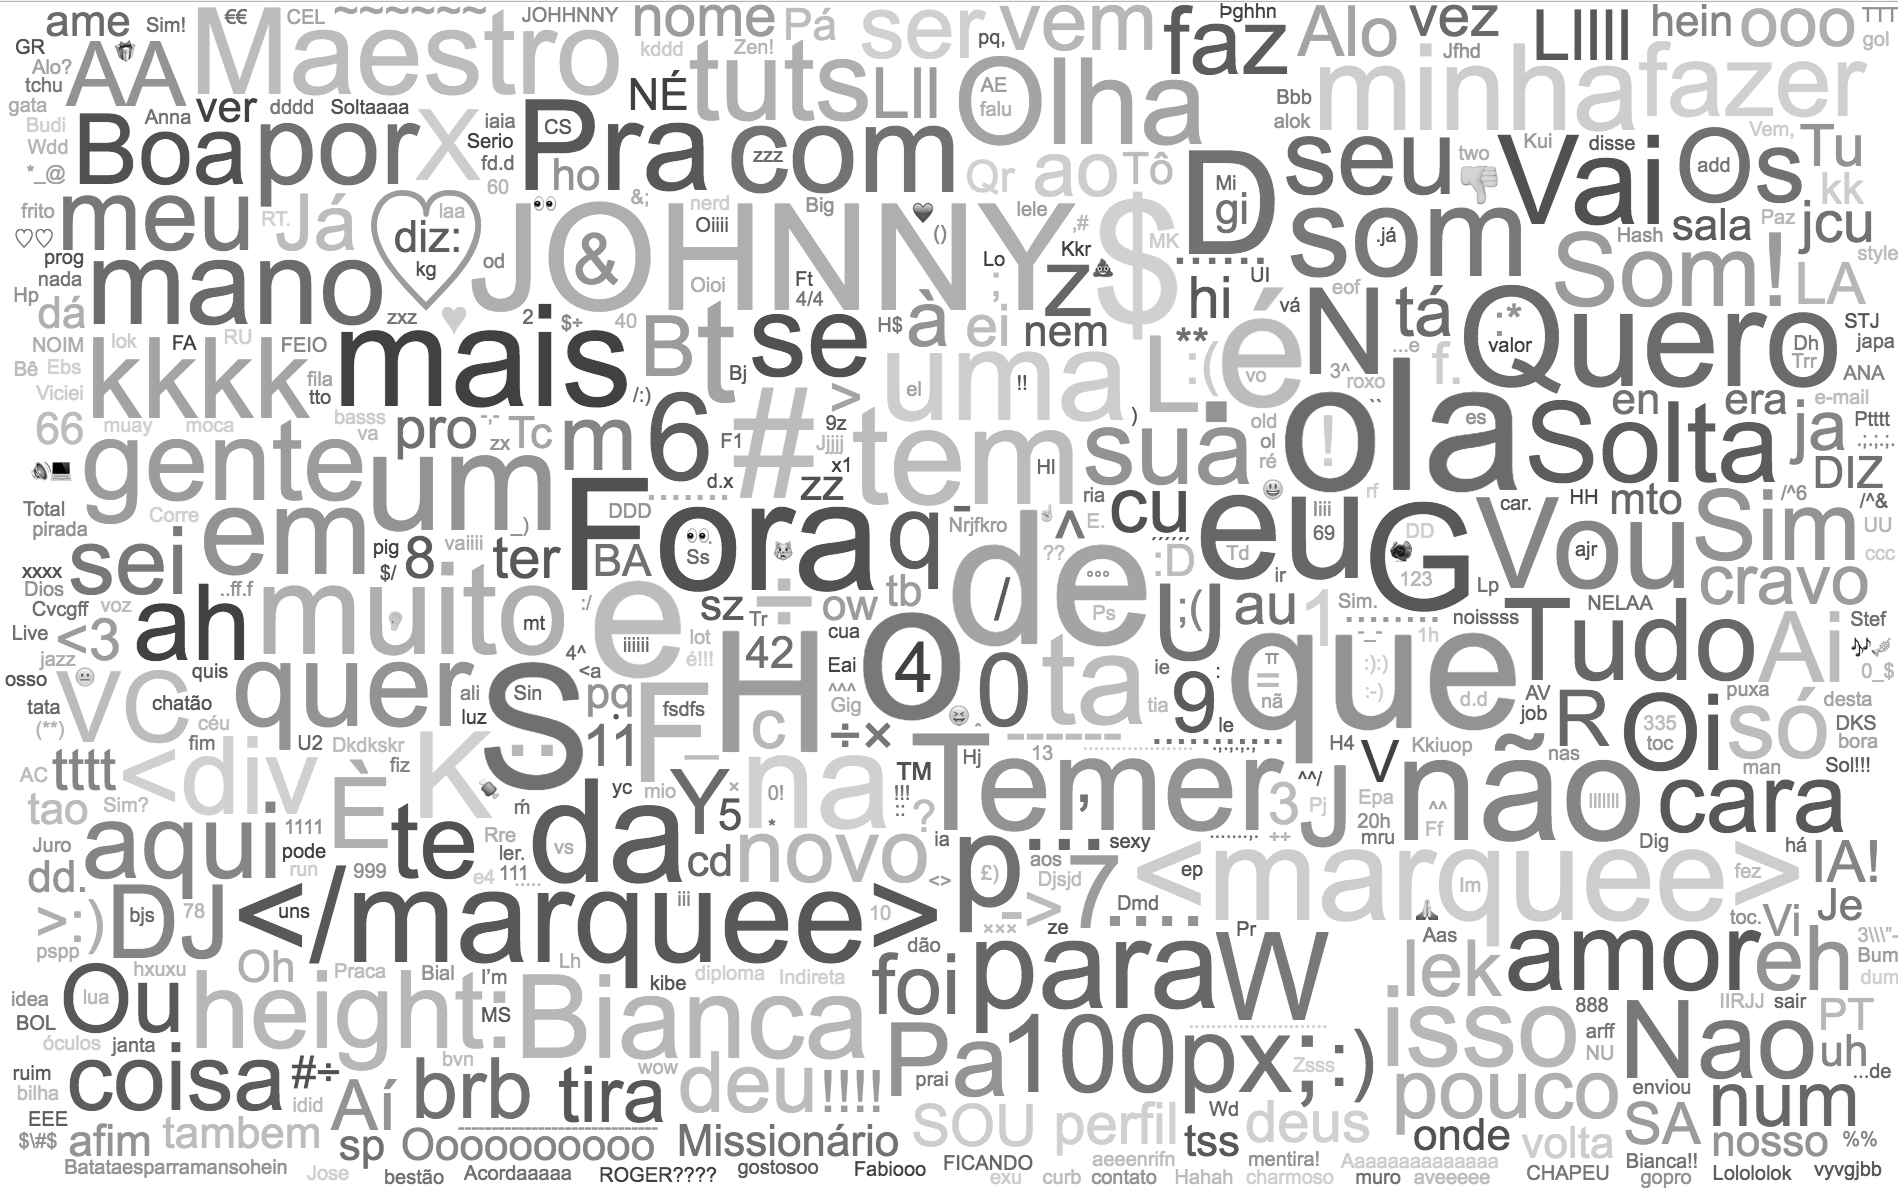
\includegraphics[width=1\linewidth]{pictures/cap3/wordcloud_pb}
\caption{Nuvem de tags gerada pelas palavras utilizadas nas performances analisadas. (Gerada pela autora utilizando a ferramenta Word Cloud).}
\label{fig:cloud}
\end{figure}

A análise revelou que uma grande quantidade de \emph{tokens}, eram palavras de apenas um caractere, que representavam cerca de 19 dos 30 tokens mais usados. Nós acreditamos que isso se deu pela natureza do projeto, uma vez que cada caractere representava um som, então os participantes poderiam usar desta estratégia para gerar um som específico. 

%The analysis revealed that a large number of tokens are single characters which represent 19 out of the 30 most used tokens. We believe that this relates to the specific nature of the Open Band chat application which turns any single character into sounds. This indicates that intent of participants could either focused on semantic meaning or on the resulting sonorities, which we analyzed further in the thematic analysis.

\subsubsection{Análise temática}
\label{sec:thematic}

Para investigar o conteúdo das mensagens, utilizamos uma metodologia de análise temática proposta por Braun e Clarke \cite{Braun2006}. Inicialmente fizemos uma análise da função linguística das mensagens, e posteriormente analizamos fatores mais relacionados ao seu conteúdo semântico.

%We analyzed the message log data using a thematic analysis following the methodology proposed by Braun and Clarke~\cite{Braun2006}. The analysis was conducted at two levels, one looking at the function of the messages, the other looking more closely at the semantic content.

%\subsubsection{Functional analysis}

Inicialmente, identificamos dois grandes grupos de mensagens, um com mensagens com conteúdo semântico explícito, e outro cujas mensagens não pareciam ter conteúdo semântico. As mensagens do primeiro grupo foram divididas nos seguintes grupos:

%We first identified two major groups of messages, depending on whether they included explicit semantic content or if their content was not semantical. The semantic messages were categorized according to their functions, as follows:

\begin{description}
\item[Fática] -- mensagens utilizadas com a principal função de testagem do canal, como:``Oi", ``Olá", etc.
\item[Metelinguística] -- mensagens que referenciavam o projeto ou a perfromance propriamente dita, como comentários e elogios, por exemplo.
\item[Denominante] -- mensagens que identificavam indivíduos, que podiam ser membors da audiência ou celebridades.
\item[Política] -- mensagens com conteúdo político.
\item[Onomatopaica] -- mensagens com onomatopéias em português ou palavras representando sons.
\item[Risadas] -- mensagens com expressões de risada, um tipo específico de onomatopéia, que foi separado do grupo pela quantidade significante de mensagens. 
\item[Declarações] -- declarações ou afirmações em geral; esta categoria inclui um conteúdo discursivo mais variado.
\item[Código] -- mensagens com códigos de programação ou comandos para mudar os sons.
\item[Emoticons] -- mensagens com emoticons pictóricos, que não eram mapeados em sons, e mensagens formadas por emoticons desenhados por caracteres.
\end{description}

As mensagens de conteúdo não semântico foram divididas em três sungrupos:

\begin{description}
\item[Letras únicas] -- mensagens consistindo de apenas um caractere.
\item[Padrões] -- mensagens que incluíam repetições de caracteres ou de sequências de letras, como um loop de letras.
\item[Aleatórios] -- sequências de caracteres sem lógica.
\end{description}

\begin{figure}[ht!]
\centering
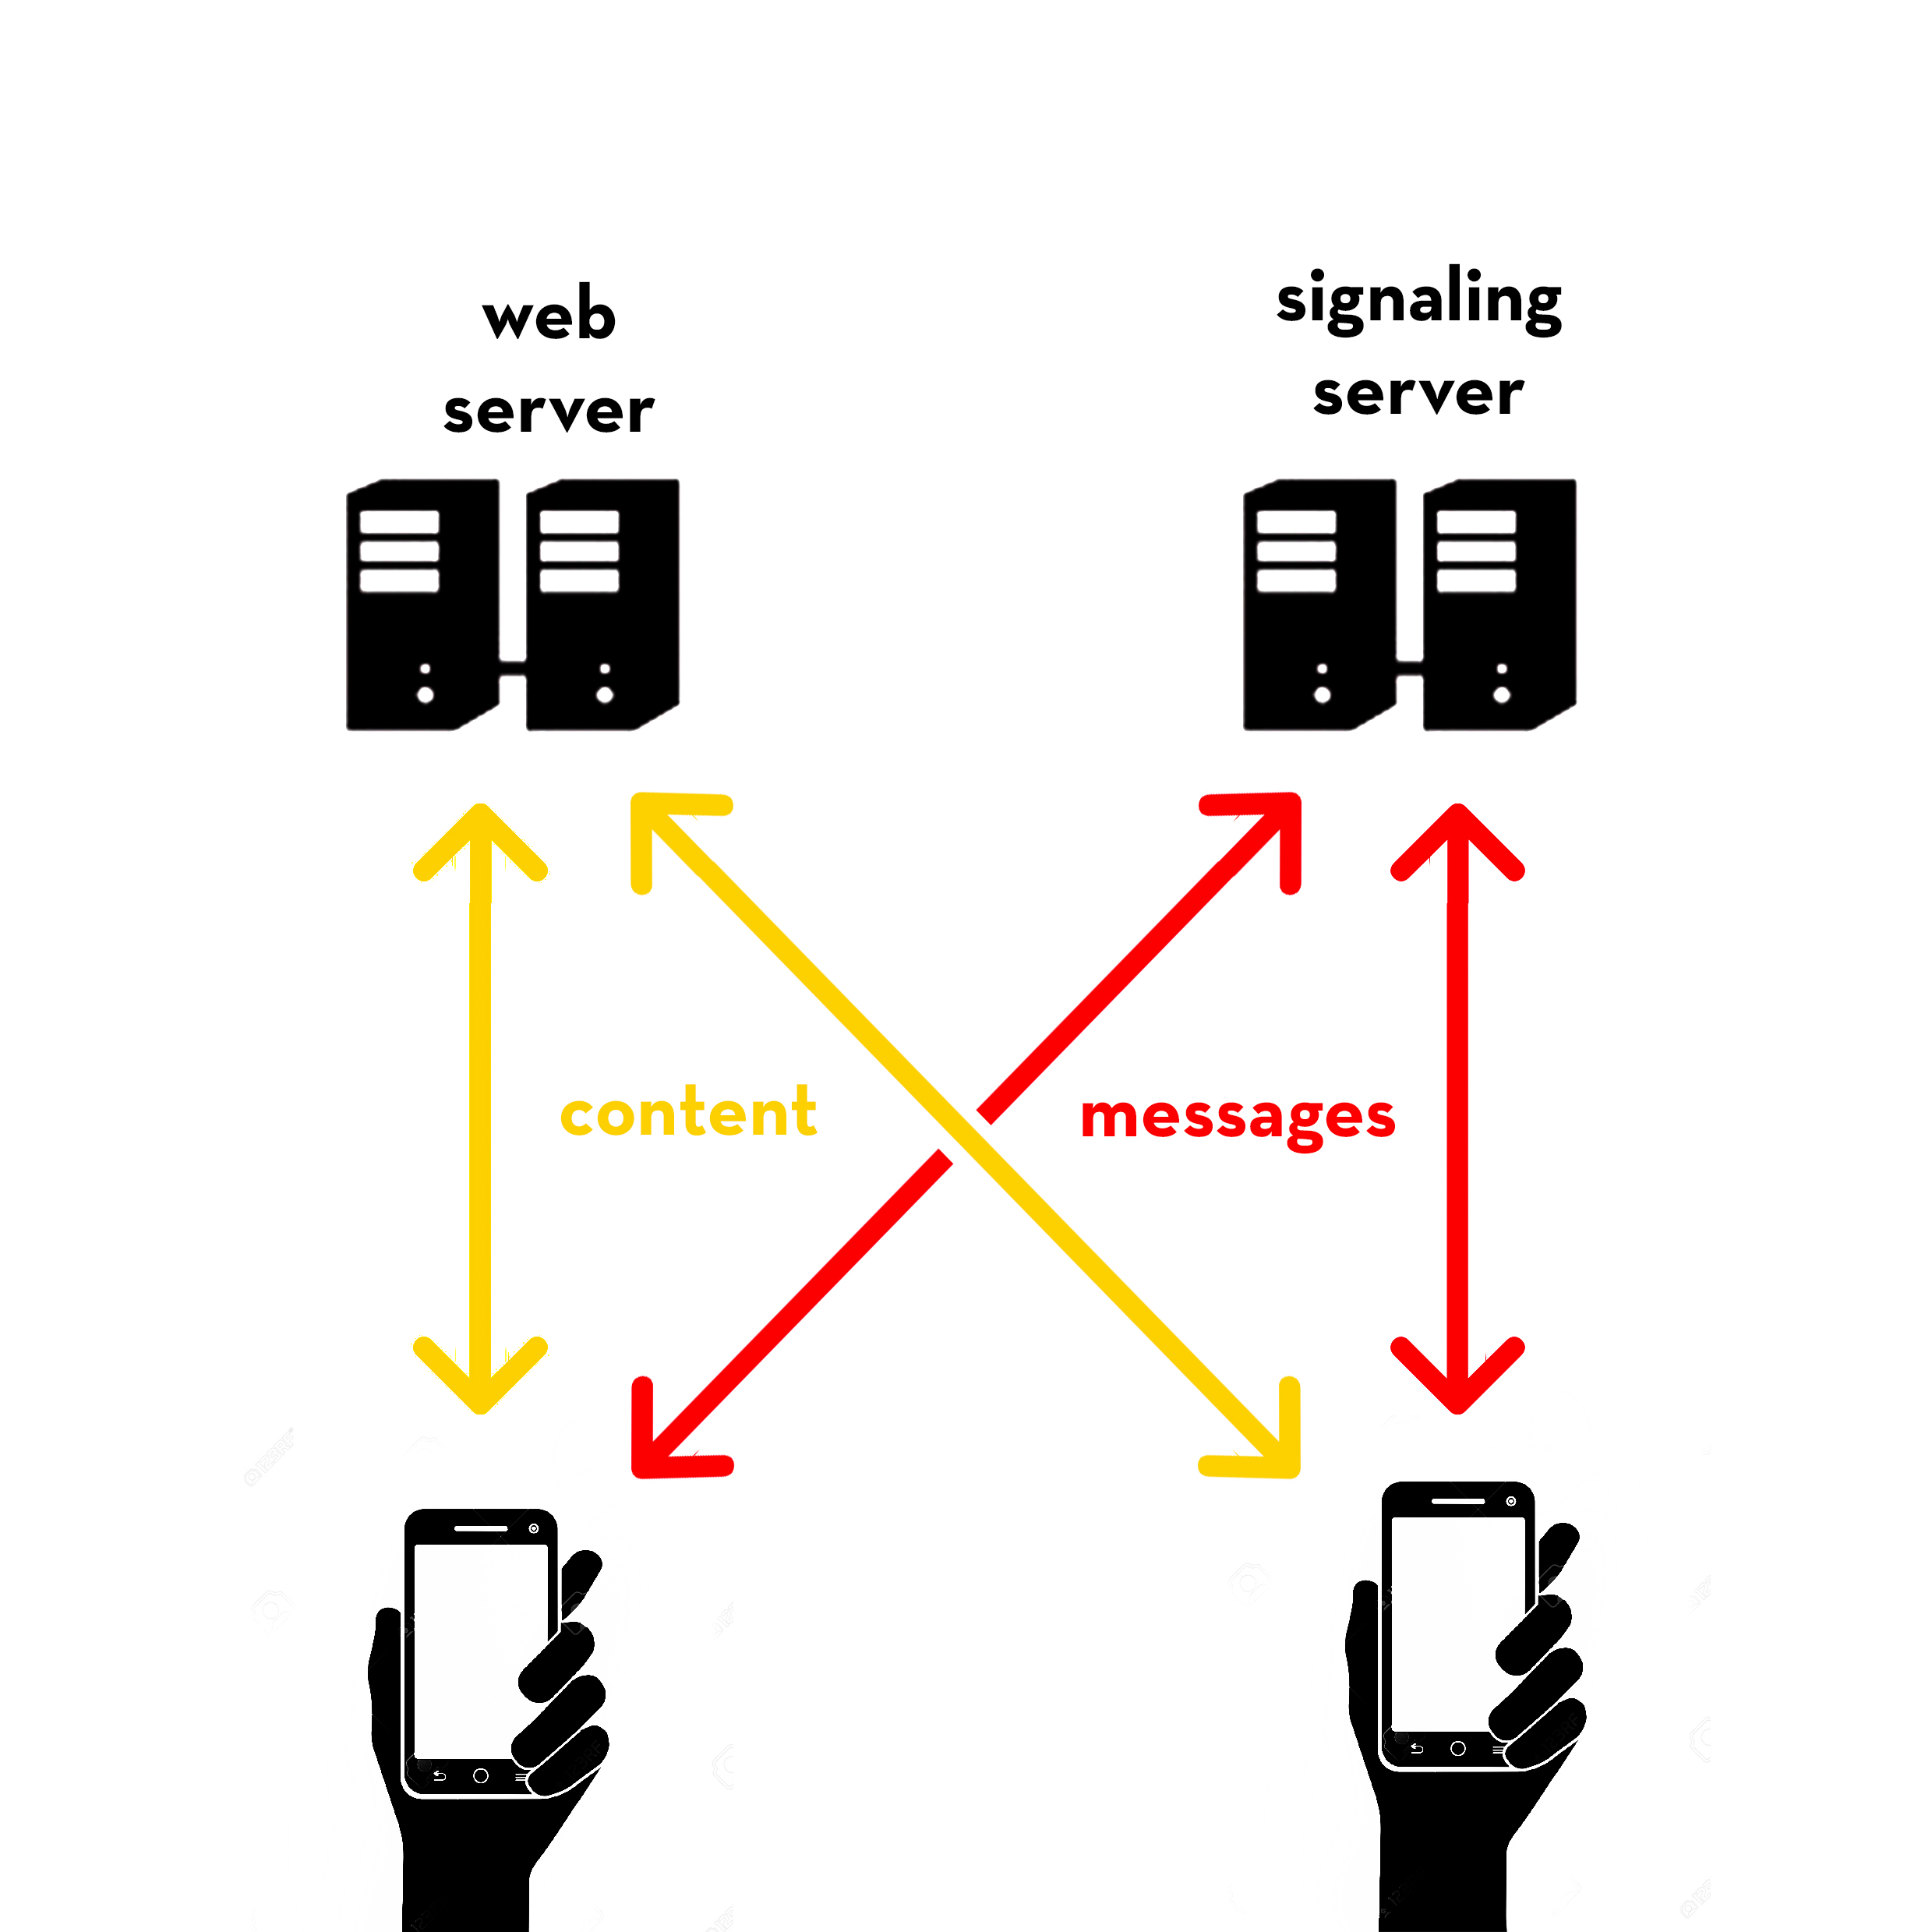
\includegraphics[width=1\linewidth]{pictures/server.jpg}
\caption{Gráfico mostrando as proporções dos temas recorrentes nas performances.}
\label{donut}
\end{figure}

O gráfico representado na Figura \ref{donut} mostra a proporção de mensagens em cada tema identificado na média das performances. De uma maneira geral, podemos notar que a mair quantidade de mensagens em todas performances foram as mensasgens de caracteres sozinhos. Nós pudemos também notar que as audiências tiveram comportamentos diferentes com relação à proporção de temas durante as performances. Por exemplo, na performance p1, os caracteres sozinhos foram mais explorados, enquanto na p3 foram menos, mensagens de conteúdo de código foram mais utilizadas na p3, onde a audiência era de cientistas da computação.

 %the proportion of the messages in each of the identified themes considering all the performances on average. Overall we can see that messages containing a single character is the most dominating theme. We can note that the audience had different behaviors in respect of the proportion of themes used during the performances. For example, much more exploring "single character'' messages in p1 and less in p3, and much more use of "code'' in p3.  

Depois de categorizar as mensagens em temas de acordo com suas funções linguísticas, fizemos uma nova análise temática, desta vez procurando buscar mais especificamente mensagens de suporte ou crítica, e também com a tentativa de perceber diferenças de comportamentos entre os diferentes conjuntos de samples. Nós identificamos os seguintes temas\footnote{Os temas não são exclsivos, podendo ser aplicados a mais de uma menagem, número total de mensagens entre parêntesis}: sem sentido (1989), slogans (180), questões (73), bullying (77), imperativo (99), auto-presença (81), reclamações (89), amor (84), humor (284), música (174), satisfação (518), and teste/condução (237). Examples incluem slogans (e.g. ``Do it"), amor (e.g. ``Paz e amor"), expressões de auto-presença (e.g.``Estou online"), referencias a outros músicos (``Lady gaga") e programas de TV (``Winter is coming" referência à série Game of Thrones), questões (``tem alguém aí?"). 

%After categorizing the messages into functional themes, we further analyzed their content to search for differences in expressions of support from the audience and how the sample packs affected the nature of the messages. We identified  the following (non exclusive) themes (total number of messages reported in brackets): senseless (1989), slogan (180), questioning (73), bullying (77), commanding (99), self-presence (81), complaining (89), love (84), humor (284), music (174), satisfaction (518), and testing/conduction (237). Examples include slogans (e.g. ``Do it"), love (e.g. ``Paz e amor": `` Peace and love"), expressions of self-presence (e.g.``I'm online"), references to musicians (``Lady gaga") and TV shows (``Winter is coming" referring to the Game of Thrones series), questions (``Is there anybody out there?"). %Some out of context copy/pasted text also appeared on the logs now and then.

\begin{table}[ht!]
\tabcolsep8.1pt
\caption{Tabela de frequência de mensagens em cada performance (p) e cada pacote de samples (sp)}{
\begin{tabular}{ c|c|c|c|c|c  }
		& \multicolumn{4}{ c| }{Performance} \\ 
  Pacote de samples & p1 & p2 & p3 & p4& TOTAL\\ \hline     
  sp0	&613 & 430 & 126 & 385 & 1154\\
  sp1	&20 & 81 & 39 & 135 & 275\\
  sp2	&142 & 82 & 143 & 64 & 431\\
  sp3	&783 & 256 & 286 & 139& 1464 \\ \hline
  TOTAL	&1558& 849 & 594 & 723& 3724\\
\end{tabular}}
% \begin{tabnote}
% Crosstable of Message Occurrence Per Sample Pack (sp) and Performances (p).
% \end{tabnote}
\label{tbl:perf_sample_xtab}
\end{table}

%\subsection{Link Between Message Content and Sample Pack}

Para investigar como os conjuntos de samples afetaram a nataureza e o conteúdo das mensagens enviadas pelos participantes, nós separamos as mensagens enviadas em cada conjunto de samples (ver Tabela \ref{tbl:perf_sample_xtab}). No total, foram 3724 mensagens enviadas no total pelo sistema. 

%In order to investigate how the various sample packs affect the nature and content of messages sent by participants, we broke down the amount of unique sent messages according to the sample pack (sp) to which they were associated (see Table~\ref{tbl:perf_sample_xtab}). In total, there were 3724 written messages sent during all four performances with various proportions for each sample pack. 


\begin{figure}
\centering
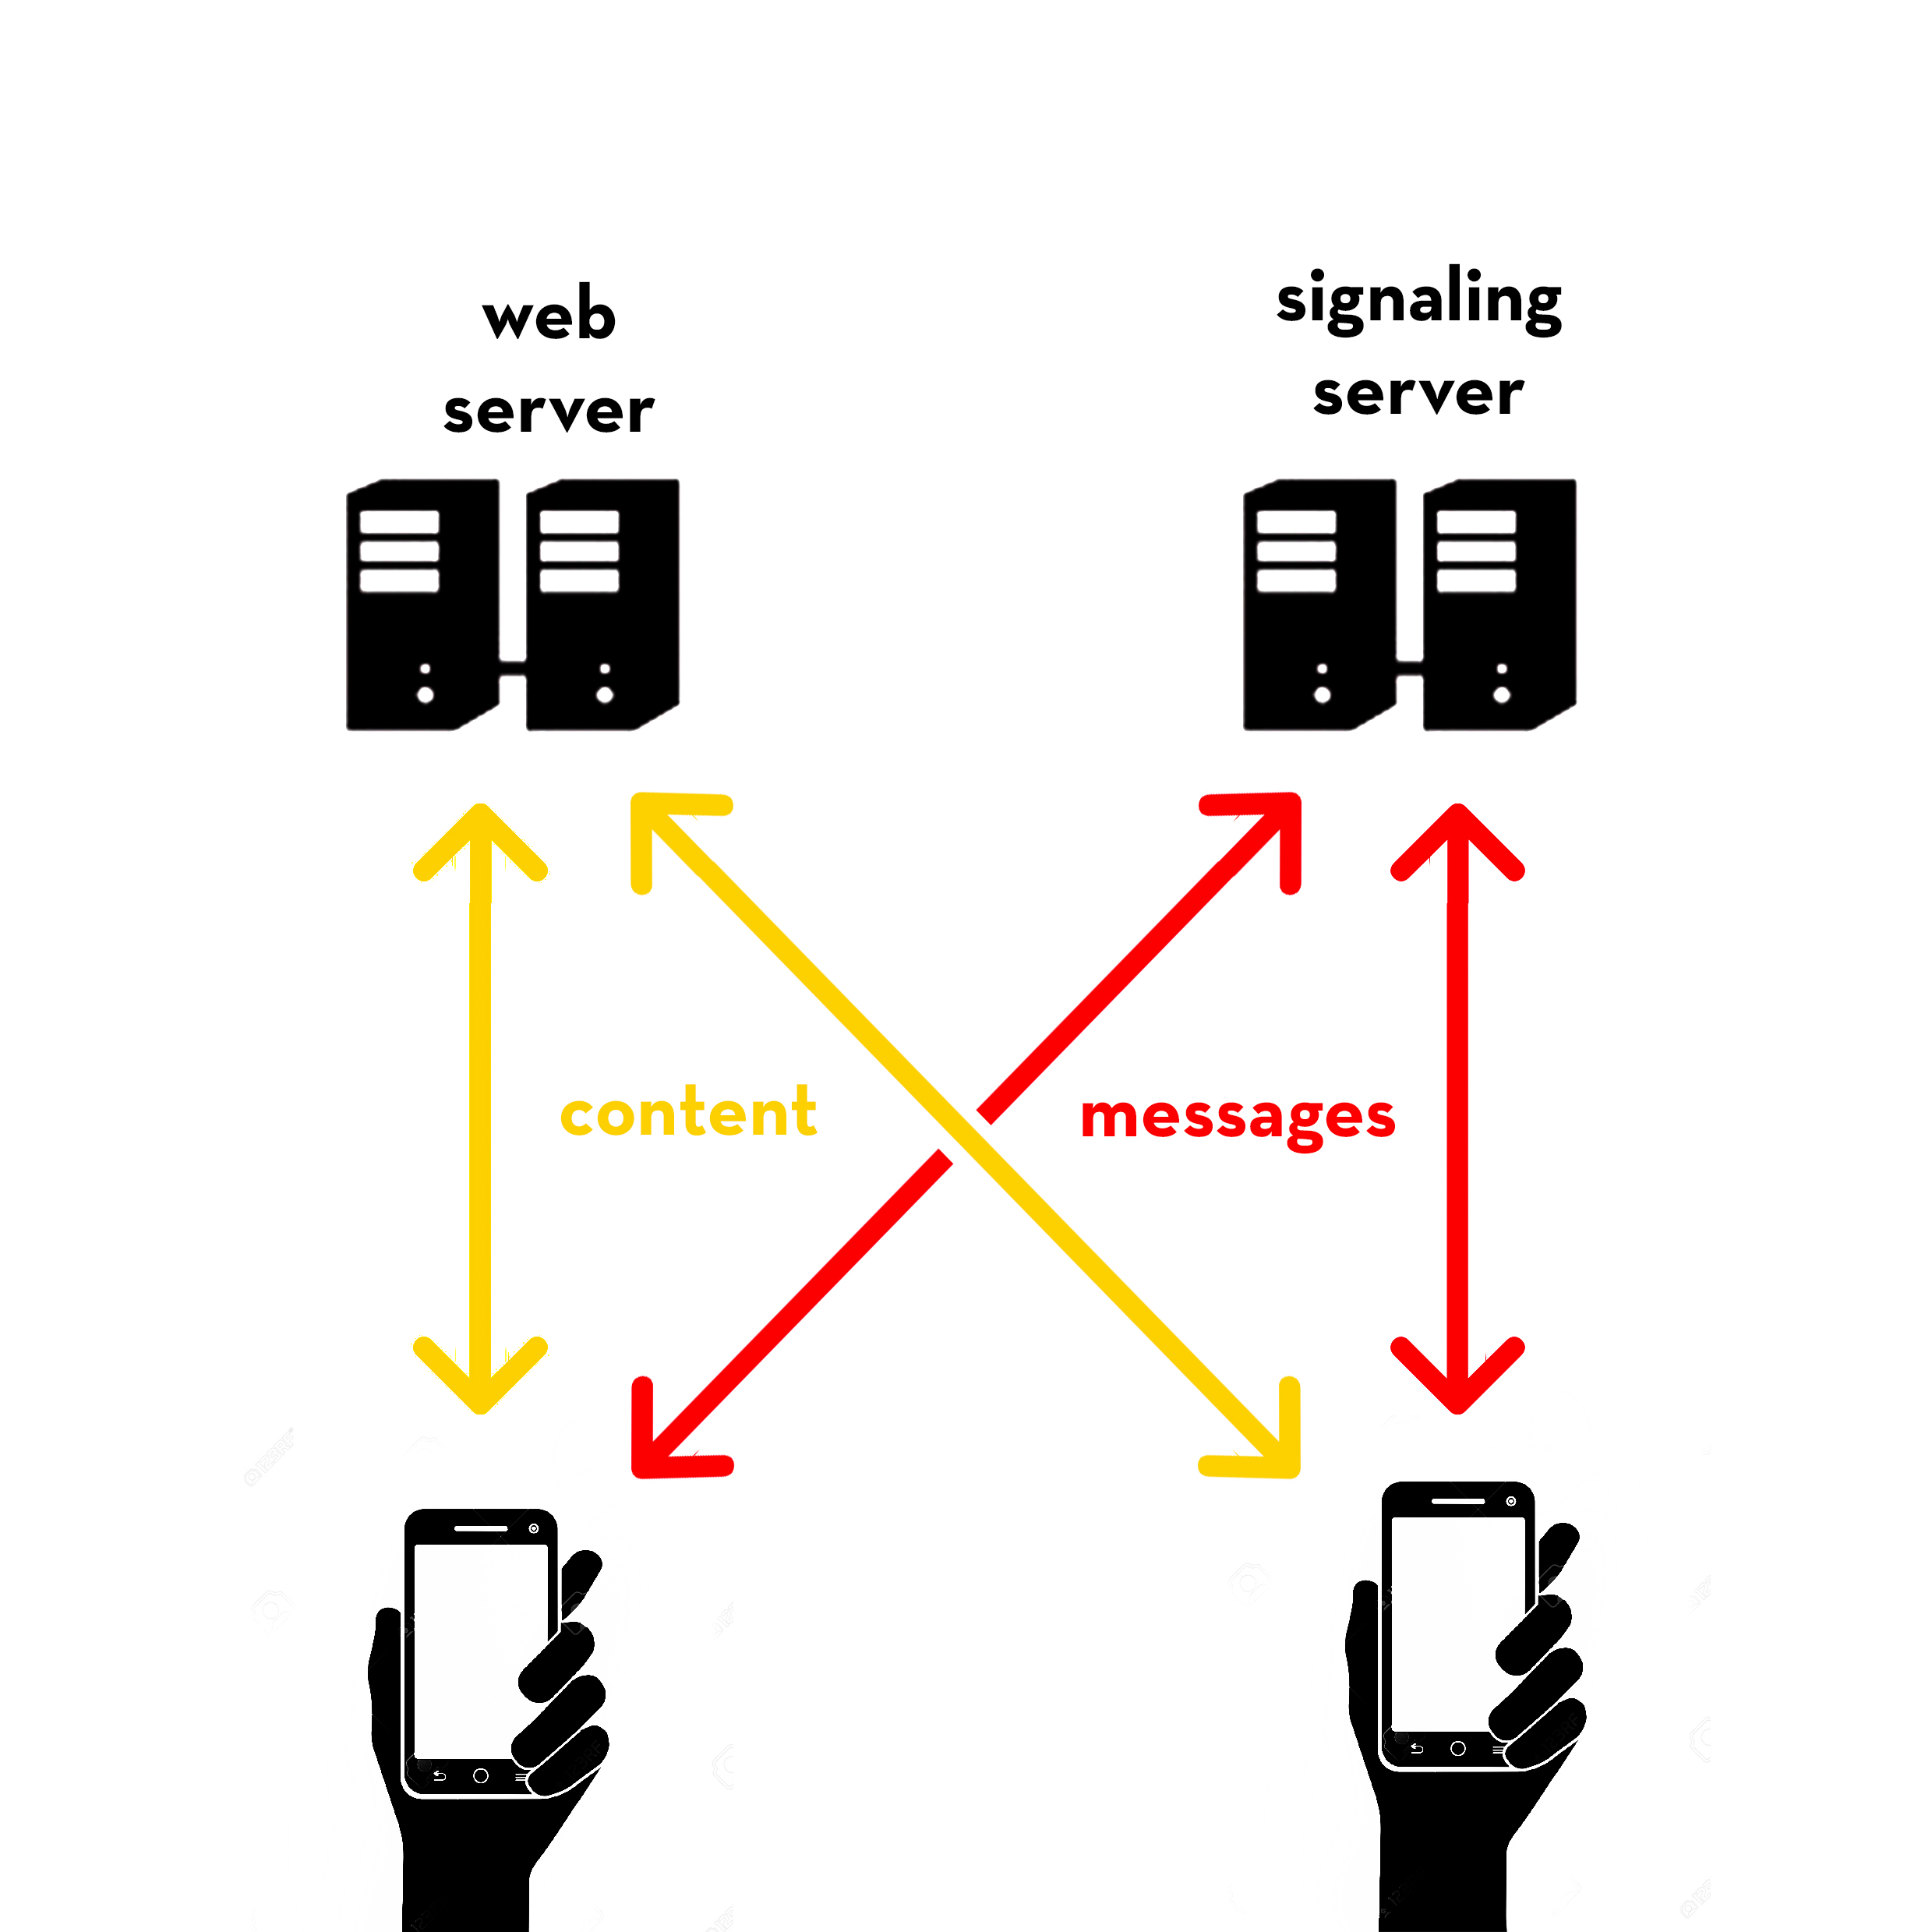
\includegraphics[width=1.1\linewidth]{pictures/server.jpg}
\caption{Frequências de conteúdos por paote de sample.}
\label{subj_themes}
\end{figure}

A Tabela \ref{subj_themes} apresenta a frequência dos temas entre os conjuntos de samples. Nós usamos análise estatística para checar se haviam diferenças entre a frequência dos temas de acordo com a mudança de conjunto de samples durante as performances. Como a quantidade de mensagens e o tempo de cada conjunto de samples era variável entre as apresentações, comparamos as frquências dos temas utilizando um teste qui-quadrado de independência. Como referência, utilizamos testes estatísticos descritos em \cite{beasley1995multiple} e \cite{garcia2003cellwise}. 

%Table \ref{subj_themes} presents the content theme frequencies across sample packs. Several differences can be noted and their significance was tested using statistical analyses. A Chi-square test of independence was calculated to compare the theme frequencies across sample packs. A significant interaction effect was found ($\chi^2$ (33) = 181.97, $p < .00001$). We performed the post-hoc test described in \cite{beasley1995multiple} and \cite{garcia2003cellwise} using Bonferroni adjusted alpha levels of 0.001.

\begin{figure}
\centering
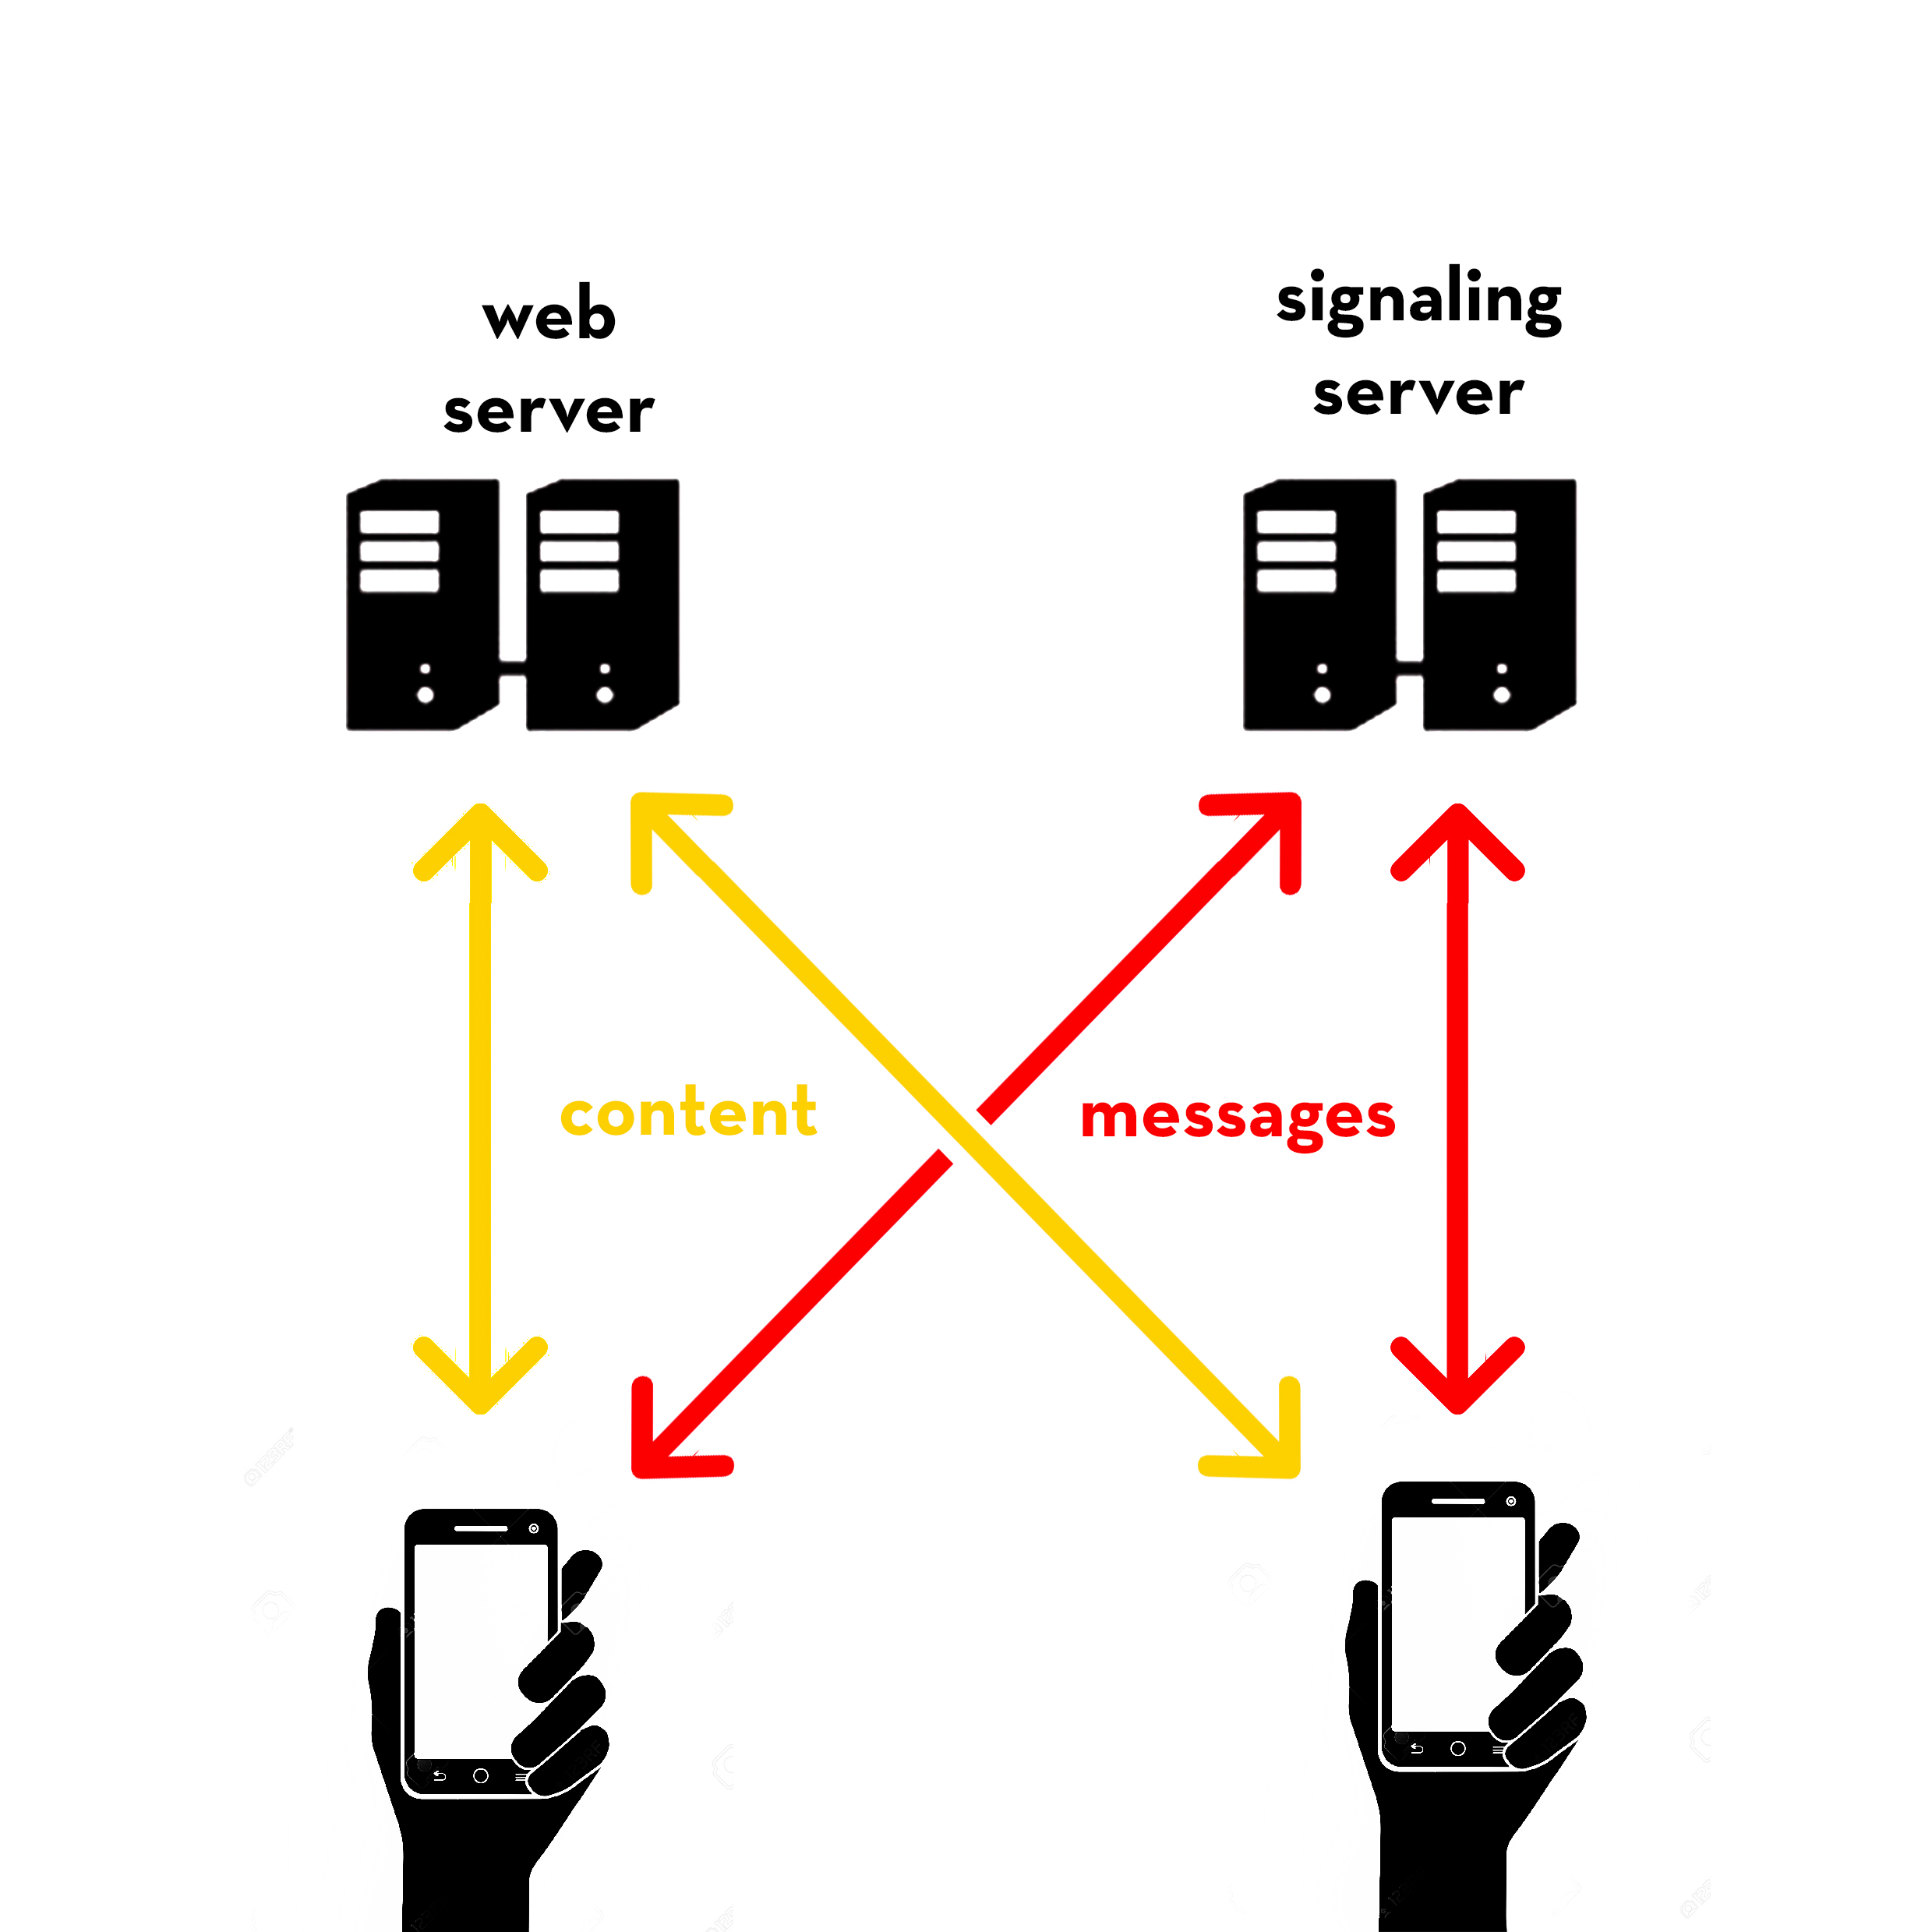
\includegraphics[width=1\linewidth]{pictures/server.jpg}
\caption{Variação na frequência de temas entre pacotes de samples. O tamanho dos círculos representa o tamanho do resíduo padrão (quanto maior o círculo, maior a diferença de frequência). A gradação de cor representa diminuição (vermelho) e ampliação (azul).}
\label{fig:bblplot2}
\end{figure}

A Figura \ref{fig:bblplot2} mostra as variações entre frequências de temas entre pacotes de samples, expressa pelo tamanho do resíduo padrão. As diferenças mais siginficativas foram encontradas entre os conjuntos sp0 e sp2. no caso do conjunto 0 (galáxias), mensagens sem sentido foram mais frequentes do que nos demais samples, e mensagens de amor menos. Isto talvez possa ser explicado pelo fato de que os sons mais estranhos estivessem nos caracteres especiais e numerais, fazendo com que os participantes explorassem efeitos sonoros utilizando esses caracteres, que criavam um contraste com os demais sons vocais. Quanto ao sp1 (percussão e acordes), não houve diferença significante, isso pode ser porque ele foi usado menos tempo durante todas as performances, por desejo dos próprios condutores, pois os sons eram mais repetitivos e tradicionais. O conjunto sp2 (colaborativo) apresentou mais mensagens de amor e menos mensagens sem sentido, o que pode ser devido ao fato de não haer uma co-relaçnao esperada entre sons e letras. Isso pode ter feito com que os participantes usassem mais discurso formal ao invés de experimentarem com padrões de ritmo. De fato, os conjuntos sp0, sp1 e sp3 foram produzidos por um método mais rigoroso de tradução intersemiótica, e foram os que levaram a mais experimentação fora do campo do discurso nas performances analizadas. 

%Figure~\ref{fig:bblplot2} displays the sources of variations of theme frequency across sample packs expressed as the size of the standardized residual. The post hoc analysis showed that significant differences of theme frequency occurred for Sample Packs 0 and 2, and for Sample Pack 3, to a lesser extent. With sp0 differences were obtained for the themes 'Love', 'Senseless' and 'Testing/Conductor' ($p < .001$). As Figure ~\ref{fig:bblplot2} shows, 'Love'-themed messages were less frequent for sp0 while 'Senseless'-themed messages occurred more frequently. This may be explained by the fact that for this sample pack, special characters were  mapped to sound effects creating unexpected contrasts compared to letters that were associated to vocal sounds. Participants may have preferred to use the special characters for these reasons leading to a more frequent occurrence of messages without semantic meaning (senseless).

%No significant changes were found for sp1. This may be because this sample pack was on overall less used for musical purposes, given that its sounds are repetitive and conductors preferred to use the pack for introduction to the system and short durations. Contrary to sp0, for sp2 'Love'-themed messages were used more frequently and there were less 'Senseless' messages in this sample pack. This may come from the fact that for this sound pack there is no expected association between letters and sounds. Participants may hence have employed a more discursive style instead of exploring letter to sound association in a rhythmic way like for other sample packs. Indeed the sample packs sp0, sp1 and sp3 which were composed using a rigorous inter-semiotic translation approach (see Section ) lead more consistently to non-semantic expressions in the chat system, contrasting with sp2 which includes sounds composed collaboratively. For sp3, the only significant difference was related to the 'Testing/Conductor' theme. As sp3 was used mostly at the end of the pieces, this is connected to the commands entered by conductors to direct the closure of the performances.

Não houve nenhuma variação significativa na frequência dos temas ``satisfação'', ``humor'' e ``reclamações'' entre os pacotes de samples, o que pode indicar que a escolha dos conjuntos não influenciou a esperiência hedônica dos usuários de uma maneira geral

%There weren't any significant theme frequency variations for 'Satisfaction', 'Humor' and 'Complaint' messages between sample packs. This may indicate that the choice of sample packs did not influence the overall hedonic experience of the participants.



%\subsection{Design}

%Various text-to-sound mappings were investigated throughout the development of Open Band: by (i) mapping letters to sounds using sample-based synthesis ~\cite{Stolfi2017} following a procedure of inter-semiotic translation~\cite{JulioPlaza1969}, or by (ii) using web audio synthesis following an isomorphic relation between the sound spectrum and the letters~\cite{Stolfi2017b}. In both cases, the mappings between the letters and the sounds were established a priori by the author and experimenters, so the only creative sonic control for the audience consisted in proposing combinations of sounds over time. Although analyses of data collected during performances indicated that the experience was fun and engaging for the audience~\cite{Stolfi2018}, we found that the capabilities of the system to support creative musical composition were limited due to the constraints and limited sonic agency. 


\subsubsection{Conclusões}

Um dos nossos objetivos era de prover uma plataforma para livre expressão da audiência, como uma ``web ágora''. A diversidade de temas que surgiram nas análises indicam que este objetivo foi atingido, uma vez que os participantes expressaram diversas posições e discutiram temas que variaram de amor a opiniões políticas.

A análise temática das mensagens, revelou um grande grau de suporte dos usuários, que pudemos medir pela quantidade significante de mensagens e satisfação (cerca de 14\% de todas mensagens). A quantidade de mensagens também indica um grande engajamento do público, com mais de mil mensagens enviadas a cada performance (ver tabela \ref{tab:msgtype}). Esses dados indicam que a plataforma foi acessada com facilidade e acessibilidade, mesmo em casos onde a audiência não tinha necessariamente conhecimentos musicais prévios. 

%One of our design goals was to provide a platform for free audience expression as a web ``agora". The various themes which emerged from the analyses endorse this idea as participants felt free to discuss subjects ranging from love to political opinions.

%The thematic analysis revealed a high degree of appreciation and support from participants; the second most frequently occurring theme was 'Satisfaction' with 518 messages across performances (14\% of all messages). Log data analyses revealed that participants actively engaged in the performances as over a thousand messages were played in each performance (see Table \ref{tab:msgtype}). Such behavior and the expressions of support in the chat communication are signs that the tool was easily accessible by audience members and that no previous musical knowledge is necessary to engage with it.

Ficou claro que a interface de chat encorajou os participantes a usar a plataforma como um meio de comunicação para conversaerm entre si, mas apesar das semelhanças que o sistema pode ter com outros sistemas de comunicação online, quase metade das mensagens escritas não tinham significado semântico. Essas mensagens, que dividimos em três sub-categorias (caracteres sozinhos, padrões e aleatórias) indicam que a audiência também utilizou o sistema para explorar o sistema de forma musical, explorando ritmos e sons de maneira estética.

%The two categories of semantic and non-semantic messages appear in almost equal proportions across performances. It is clear that the chat interface encouraged participants to use Open Band as a way to communicate with each other. Screen projection of the chat made Open Band a compelling means for posting messages to be shared with ones's entourage, as is done in other social media platforms. However, although Open Band's interface shares similarity with other web-based platforms for verbal communication, approximately half of the messages did not show any explicit semantic content. These messages, which can be divided into three sub-categories (single characters, patterns, and random-like) point to the exploration of the musical potential of Open Band, since they served to engage with the system's sonic features and to performatively explore these features.

Tocar repetidamente a mesma letra pode ser visto como uma forma de testar o sistema, mas também como forma de disparar sons em um ritmo específico, e também de ouvir aquele som único no meio da massa sonora composta pelas frases. é similar à função fática no contexto semântico, como aponta Jakobson que serve principalmente para estabelecer, prolongar ou encerrar a comunicação \cite{Jakobson}. Também permite com que os usuários reconheçam a sua contribuição específica dentro da performance e reconhecer os sons individuais. Padrões, por outro lado, ou repetições de sequências curtas permitem aos participantes a criação de motivos rítmicos ou frases musicais, que também se destacam do conteúdo textual que em geral não tem muita repetição, se aproximando da linguagem musical.

%Repeatedly typing the same letter can be seen as a way to test the system and check its communicative capabilities. It is similar to the phatic function in the semantic context ``primarily serving to establish, to prolong, or to discontinue communication" \cite{Jakobson}. By repeating a same keyboard key the user could recognize the relationship between individual letters and the sounds they produce. In addition, repetition allows a clear identification of each participant's own sonic contribution within the somewhat complex flow of sounds that can be produced during a performance. On the other hand, the loop repetition of short sequences allows for the creation of rhythmic motifs that stand out from the random sonorities produced at certain moments. Finally, texts with non-semantic content produced by the almost random triggering of the keys are strong indicators of participation in performing Open Band as a music practice.

Como aponta uma das mais importantes referências da cultura moderna brasileira nas artes, o Manifesto Antropófágico de Oswald de Andrade de 1928 \cite{Andrade1928}, ``a alegria é a prova dos nove''. Nesse sentido, os dados recolhidos, assim como a observação do comportamento da audiência apontam uma evidência de que o projeto foi bem sucedido nesse sentido, com várias referências de humor, declarações de apoio e risadas registradas pela audiência. 

%Possibly one of the biggest influences in Brazilian modern culture, the 1928 ``Cannibal Manifest" from poet Oswald de Andrade~\cite{Andrade1928} presents an important standpoint for our work, ``Joy is the real proof". From this standpoint the data provide some evidence that the performances were experienced in a playful way, as there were many statements and declarations of fun and enjoyment in participant messages.

Sob outro ponto de vista, que era o de propor uma ``Obra Aberta'', nós consideramos que o sistema poderia ser mais aberto, uma vez que os usuários tinham liberdade somente para escolher o texto, mas não para fugir dos sons pré-programados pela compositora e escolhidos pelo condutor durante as performances. Em se tratando de uma audiência que não tinha necessariamente treinamento musical, essa opção foi importante para manter a consistência estética do projeto.

%From another standpoint, which was to propose an Open Work, we still consider the current system insufficient, as users have little freedom about the sounds to use since these are restricted to the ones chosen by the composer and the conductors during the performance. We maintained the control of sound production mechanisms fairly simple in favor of ease of use and intuitiveness. With such an approach the system is open to audience without prior musical knowledge, thus minimizing the amount of instructions required to participate. To maintain artistic consistency of live performances, the sample packs' choices were left to the artists facilitating the performances. %The choice of constraints was also decided to maintain the artistic consistency of the live performances in musical terms.



%However to increase the agency of participants, users should be able to map themselves the sound into letters, or at least be able to decide between broader sound options. To attempt to address this issue, we are developing as part of the Audio Commons\footnote{\url{http://audiocommons.org}} project, a new platform using the Freesound Application Programming Interface~\cite{Font2013}. The prototype, Playsound.space, is a web-based interface (Figure ~\ref{playsound}) that let users search sounds in the Freesound database using semantic queries. Future work will investigate how letters can be mapped into sounds in the Playsound platform. Combining the Open Band and Playsound frameworks may lead to new interesting applications for the re-purposing of crowd-sourced content for music making and instant messaging auditory display.


%We wanted to expand it to be a framework to be used in different musical contexts. One of our goals is to integrate the project with the audio Commons API\cite{Akkermans2011} to foster media re-purposing, creating an interface for uploading and mapping sounds to the letters. For the web audio synthesis version, we aim to develop form to control the base frequencies and rhythm trough gestural interfaces, to enhance the musical possibilities given to the audience.

Apesar do projeto Banda Aberta ter se mostrado interessante como experiência participativa e projeto de performances, os resultados sonoros e as possibilidades criativas de produção musical ainda não estavam suficientes para suprir minhas necessidades pessoais como um instrumento para performance ao vivo. Durante minhas atividades práticas musicais, tive a oportunidade de tocar com o sistema em performances de improvisação livre em algumas situações, como na apresentação para o festival aMostra Sonora. Durante a performance, onde utilizei também um patch de Pure Data que desenvolvo há cerca de 10 anos, percebi que a quantidade de sons não era suficiente para proporcionar uma variação sonora satisfatória em performances longas. Para isso, precisaria também de algo que realmente servisse como um intrumento musical, e não somente como sampler. a partir daí, surgiu a idéia de um projeto que envolvesse a API do Freesound, para ampliar as potencialidades sonoras, que vamos descrever na próxima seção desta tese.


%- amostra - limitação de sons para performances longas
%- audio mostly - feedback atrapalhou a performance


\end{otherlanguage*}


    % Segundo capitulo de Resultados
    \begin{otherlanguage*}{brazil}

\section{Playsound}

O desenvolvimento da plataforma Playsound.space começou durante o meu período de estágion o Centre for Digital Music (C4DM) na Queen Mary University of London (QMUL)\footnote{O Estágio aconteceu de junho de 2017 a maio de 2018 e foi financiado pelo Programa de Doutorado Sanduíche da CAPES}, onde tive a oportunidade de participar do grupo de pesquisa ligado ao projeto Audio Commons\cite{Font2016}. Depois de desenvolver o projeto Banda Aberta, o desejo era de trabalhar no desenvolvimento de um sistema que pudesse ser utilizado como um instrumento musical, que fosse capaz de produzir uma gama rica de sonoridades e não mais somente uma plataforma para tocar sons pré determinados. 

A iniciativa Audio Commons visa trazer conteúdo sonoro em Creative Commons (CC) para artistas e indústrias criativas. Licenças CC fornecem uma maneira padronizada para dar permissão ao público no compartilhamento e utilização de trabalho criativo em condições definidas pelos criadores de conteúdo, que pesquisa formas de aproveitamento e utilização de serviços online de distribuição de conteúdo sonoro com licenças em Creative Commons footnote{\url{https://creativecommons.org/}}. O projeto é financiado pela união Européia e tem entre seus obetivos, desenvolver uam ontologia para sons, e criar um mecanismo mediador para pesquisar sons de diversas fontes como as bilbiotecas Freesound.org, um grande repositório de samples; Europeana.org, que reúne um acervo de gravações históricas de diversas intituições européias e Jamendo.com, que reúne músicas novas produzidas em licensas livres.


Nosso principal domínio de aplicação é a improvisação musical que é definida como uma atividade musical autônoma \cite{Canonne2016} que geralmente leva a situações pluralistas, com ênfase no processo de tocar, e na iteração musical no momento \cite{BERGSTROEM-NIELSEN2016}. Em oposição à improvisação idiomática, como aquela praticada em algumas formas de jazz ou hip-hop, a improvisação livre pode levar à formas não metrificadas e sem escala ou tonalidade pré-determinadas, onde muitas vezes a variação de timbre prevalece\cite{Barthet:11a}. Já vinha desenvolvendo atividades em improvisação livre anteriormente, mas depois do início do doutorado, tive oportunidade de participar da Orquestra Errante, grupo conduzido pelo professor Rogério Costa que ensaia semanalmente no estúdio do NuSom na Universidade de São Paulo. 

Durante as práticas de improvisação musical que participei até agora, encontrava algumas dificuldades em utilizar softwares tradicionais como DAW patchers. Uma delas é de que muitos softwares do tipo DAW são baseados em grids temporais fixos, ou seja, existe um tempo que determina o fluxo dos acontecimentos sonoros, e embora esse tempo possa ser mudado, a estrutura rígida conflita com a necessidade da liberdade na improvisação. A estrutura em grade ou se impõe para os demais músicos, como um metrônomo, ou entra em conflito com os demais participantes. Além disso, as estruturas temporais também dificultam a criação de polirritmias. 

Softwares que se comportam como instrumentos virtuais, por outro lado, como sintetizadores e \emph{samplers} são mais fáceis de serem empregados na prática. Por serem baseados em gesto, o controle do fluxo sonoro fica a cargo do musicista, dependendo aí do tipo de controlador que ele usa, de sua expertise técnica em tocar, e da capacidade de variação timbrística do instrumento. No caso dos sintetizadores, as possibilidades de variação de sonoridade são constringidas pelos timbres oferecidos pelo fabricante ou programador, e em geral restritas a sons musicais, dentro de uma escala pré-determinada. Além disso, para se obter um bom controle de dinâmica, é recomendado a utilização de controladores externos, como teclados midi, por exemplo. Minha idéia era desenvolver algo que pudesse ser tocado em tempo real, e que permitisse mais variação sonora do que os softwares e ferramentas disponíveis no mercado.

No Contexto de novas interfaces para produção musical uma série de abordagens diferente têm sido desenvolvidas para o emprego do computador como instrumento musical na prática de improvisação livre. Exemplos incluem \emph{live coding} \cite{freeman2011collaborative} e orquestras de laptop \cite{Albert2012}. \emph{Live Coding} colaborativo ao vivo frequentemente envolve o desenvolvimento de tecnologia pra sincronização entre dispositivos \cite{Wilson2014}, que aqui não foi adotada devido à escolha estética de deixar a estrutura rítmica livre.


A ideia de tocar com uma ``paleta de sons expandida'' tem sido explorada na música desde Luigi Russolo  \cite{Merz2013} e especialmente depois da música concreta. A digitalização e a disponibilização de sons online potencializa essa ideia, como aponta Schnell:
\begin{citacao}
``In the age of digital sound databases and online music publishing services, the total disembodiment of digital sound turns into the promise of perpetual reincarnation of digital sounds through their permanent exchange and transformation."\cite{Schnell2013}
\end{citacao}

Nos instrumentos que funcionam a base de amostras de sons (samplers), as possibilidades sonoras são ampliadas pela possibilidade de utilização de sons não-musicais, ou em outras escalas, mas são dependes de se ter acesso e conhecimento de uma biblioteca grande de sons. Localizar samples em tempo real durante uma improvisação musical pode ser desafiador\cite{Xambo2018}, principalmente porque a improvisação exige do musicista uma reação espontânea e instantânea em tempo real \cite{canonne2011model}. Isso exige que o performer conheça bem e previamente os sons de uma determinada coleção, o que se torna impraticável se a coleção de sons é muito grande. Para contornar este problema, os praticantes normalmente selecionam uma amostra reduzida de sons, o que acaba também por reduzir suas possibilidades criativas durante as performances.

A digitalização do som, em conjunto com tecnologias Web e bancos de dados de áudio digital abre muitas possibilidades critativas, que como Schnell aponta, pode levar à ``promessa de reencarnação perp´tua de sons digitais através da sua permanete troca e transformação'' \cite{Schnell2013}. A utilização de amostras de sons pré-gravados é largamente empregada em uma série de tradições estéticas musicais como no emph{Hip Hop, Plunderphonics, Música Eletrônica, Música Concreta, composição de Paisagens Sonoras}. Bibliotecas online de áudio como Freesound.org, Redpanal.org, Sampleswap.org entre outras são utilizadas por compositores e produtores musicais de vários tipos de aplicações multimídia como cinema, publicidade, video games, e composições musicais \cite{Roma2013}. 

Alguns projetos desenvolvidos recentemente têm também esse norte como paradigma. O projeto API Cultor, por exemplo \cite{Ordiales2017} usa técnicas de \emph{machine learning} para prover um ambiente para re-utilização de sons de blibliotecas online. Lee et al. propõe uma ferramenta para \emph{live coding} com a API do Youtube para improvisação livre \cite{Lee}. Ao prover acesso a seu banco de dados por uma REST API \cite{Akkermans2011}, o site Freesound.org permite que musicistas e designers criem aplicativos que explorem seu conteúdo online para utilização ao vivo. BeatPush \cite{Feenstra2016}, é um exemplo de sequenciador usando esta API e o Freesound Explorer \cite{Font2016}, por exemplo, organiza os sons em uma configuração espacial por similaridade e usa cores para representar aspectos timbrais, no entanto, é uma aplicação mais voltada para navegação e exploração do que para tocar em tempo real, e não permite que os usuários selecionem sons a partir de buscas múltiplas. 


Entre diversos serviços que provém conteúdo sonoro online, uma imensa gama de sons musicais e não musicais são oferecidos pelo Audio Commons Ecossystem \cite{Font2015}. A ideia no desenvolvimento do Playsound era de ser uma tentativa de contornar essas questões, promovendo o acesso a esses sons em tempo real através da API do Freesound \cite{Akkermans2011}, oferecendo feedback visual através de espectrográficos, de uma forma que pusesse ser tocada sem um grid de tempo fixo e por usuários sem domínio de técnicas musicais.

Compor a partir de espectrogramas era uma idéia que acompanhava meu trabalho já faz algum tempo. Em 2011 publiquei um trabalho chamado UTOPIA, onde desenhava a palavra utopia através de síntese subtrativa sobre uma gravação feita de uma serra de fita em funcionamento, que era uma amostra bastante saturada. Essa idéia também voltou outras vezes no meu trabalho, na composição da peça Bandas Críticas e no processo de composição de sons para o Banda Aberta. Quando começamos a publicar os primeiros artigos a respeito do projeto Banda Aberta comecei a buscar ferramentas para conseguir imprimir os conjuntos de samples (ver figuras \ref{samplesgalaxias}, \ref{samplespercussao}, \ref{samplescolab} e \ref{samplesorquestra}) e não consegui encontrar nenhuma ferramenta pronta que pudesse gerar espectrogramas de um conjunto grande de sons que fosse acessível, então para gerar essas imagens, bem como os sites que reúnem os samples do projeto, precisamos desenvolver uma ferramenta própria, que chamamos de spectrogram player, que foi o esboço de um player a partir de spectrogramas, em JavaScript e HTML \footnote{A ferramenta foi desenvolvida em código aberto e está disponível no endereço: \url{https://github.com/arianestolfi/spectrogramplayer}}. Quando comecei a desenvolver este novo projeto, descobri que a API do Freesound já fornecia os spectrogramas dos sons de sua bilbioteca, o que era muito conveniente para o projeto, já que diminui o tempo necessário para a análise via FFT que poderia gerar os spectrogramas em tempo real. Além disso, ao oferecer os spectrogramas como imagens, a API do Freesound permite realizar a pesquisa sonora sem a necessidade de baxar os sons toda vez no computador do usuário.

Além disso, queria desenvolver uma ferramenta que não dependesse de expertise técnica ou virtuosismo, que é um dos objetivos dessa pesquisa. Assim como no projeto Banda Aberta, decidioms manter o texto como forma de interação com o sistema, mas ao invés de fazer um mapeamento de sons por letras, como no projeto anterior, aqui o texto serve como fonte para buscar informações, ao permitir a busca através de significados semânticos ou descritivos, por exemplo: ``chuva pacífica'', ``crowd noise'' ou ``raucous cockatoos''. A solução técnica foi o desenvolvimento de um sistema de busca que provém o acesso a centenas de milhares de sons em Creative Commons baseada na API do Freesound.

\subsection{Motivações}




\subsection{Desenvolvimento do Projeto}


\begin{figure}
\centering
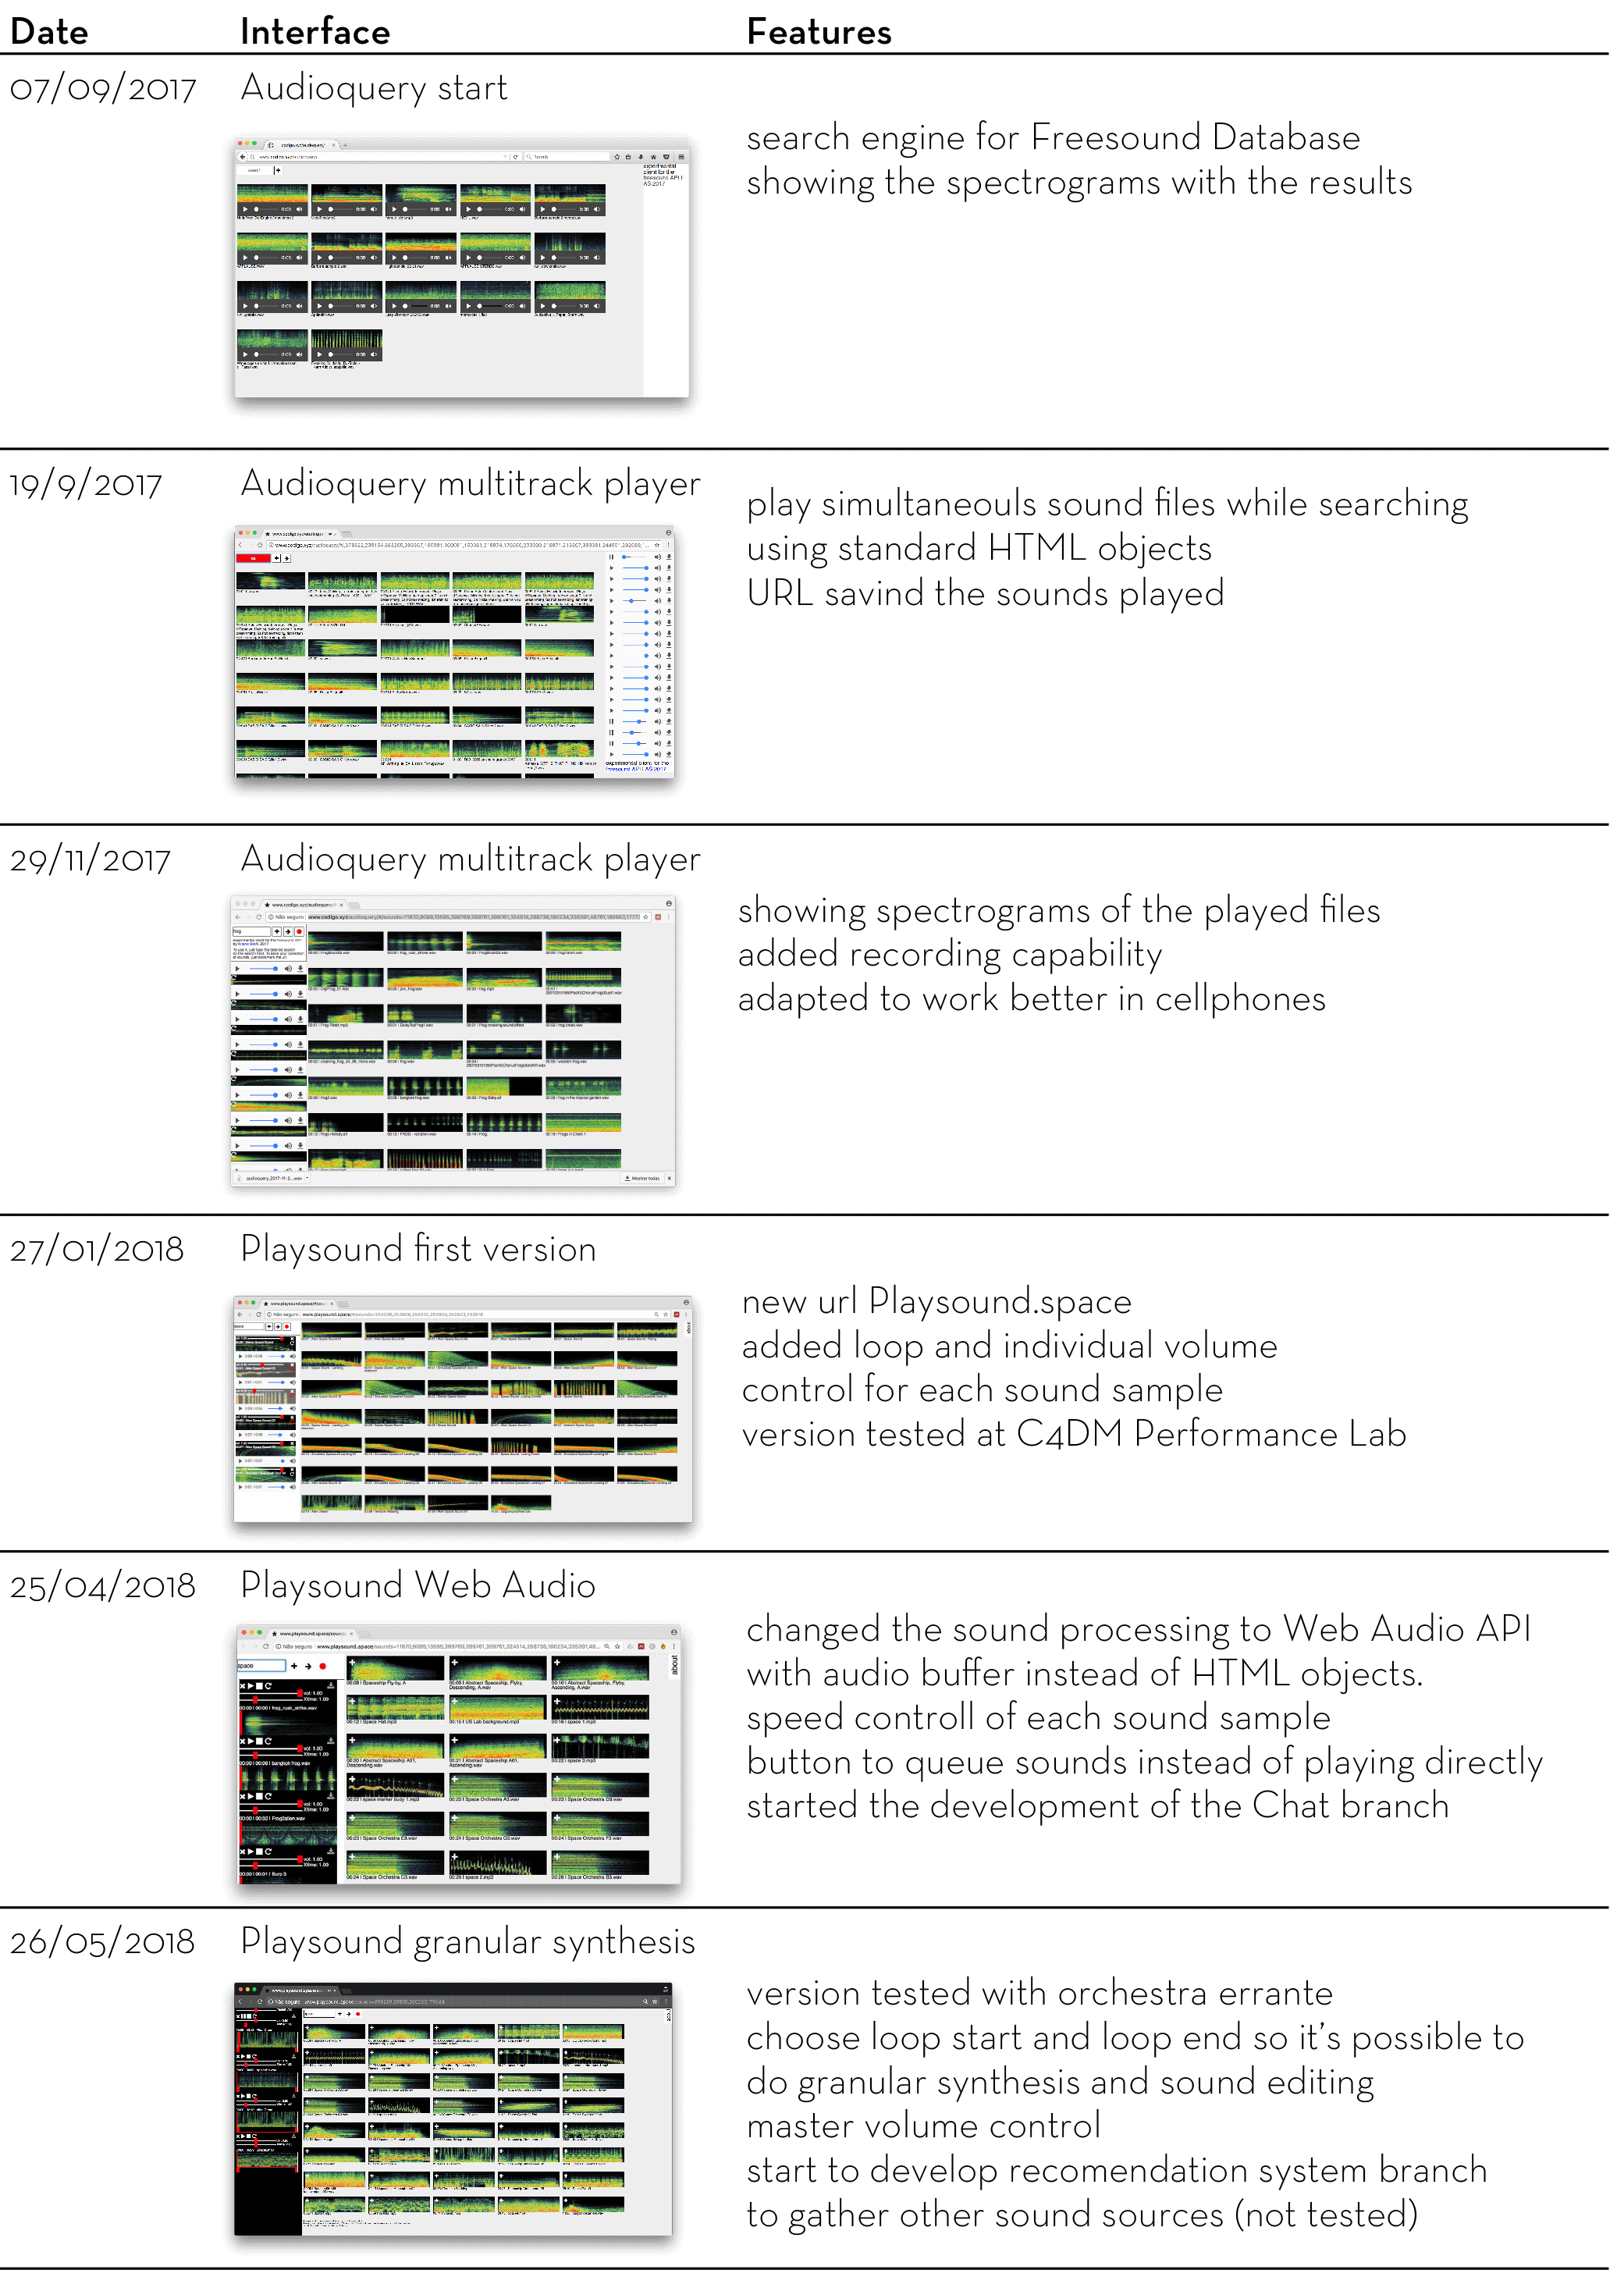
\includegraphics[width=0.8\textwidth]{pictures/playsoundtimeline}
\caption{\label{pstimeline}Playsound development timeline}
\label{fig:timeline}
\end{figure}

Comecei a desenvolver o projeto em Julho de 2018, após apresntar o Banda Aberta em alguns eventos na Europa que descrevi na seção anterior. A figura \ref{fig:timeline} apresenta os principais estágios de desenvolvimento da ferramenta de Setembro de 2017 a Julho de 2018. Utilizei novamente Lean Ux \cite{Liikkanen2014} como metodologia de desenvolvimento de software. Dentro dos princípios desse método, começamos novamente o projeto a partir de um protótipo bem simples, que era apenas um sistema de busca que mostrava o resultado como um conjunto de spectrogramas. Inicialmente, contei com a ajuda do programador Miguel Ceriani para fazer a ligação com a API do freesound.

Utilizamos como \emph{framework} Angular.js\footnote{Angular.js é um \emph{framework} em JavaScript desenvolvido pela Google que permite automatizar certos processos computacionais e facilita a comunicação com bancos de dados}. O Framework fornece o recurso de ligação de dados bidirecional, que faz com que a busca aconteça no servidor simultaneamente ao se digitar o texto na caixa de busca. Deste modo, mesmo antes de se completar uma palavra, resultados já começam a aparecer na janela do navegador. Para o processo de improvisação livre, esse recurso se mostrou muito interessante, uma vez que sons não esperados podem surgir mesmo antes de se estabelecer um vocábulo definitivo. 

Os resultados são apresentados na forma de spectrogramas, que permitem que o usuário do sistema tenha informações sobre ritmo e timbre das amostras recebidas antes de escolher o som para tocar. Os resultados são apresentados em uma matriz, que permite que se compare os sons visualmente. Apesar de a leitura dos spectrogramas não ser uma coisa corriqueira para qualquer usuário do sistema, acreditamos que um aprendizado implícito pode acontecer no simples processo de pesquisar e tocar com o sistema, quando se percebe a co-relação entre a representação gráfica das propriedades espectro-temporais dos dos sons e suas qualidades audíveis. Quando selecionamos uma imagem, o som é adicionado a uma playlist na lateral da interface.

 Assim que colocamos o sistema no ar, começamos a desenvolver recursos adicionais para transformar o sistema em um instrumento musical de fato. O primeiro recurso desenvolvido foi a capacidade de se fazer novas buscas enquanto os sons são tocados, recurso que já não existe no próprio Freesound. Em seguida, criamos um sistema de url para armazernar uma coleção de sons feita previamente. Cada som selecionado gera um código que fica registrado no endereço do navegador. Desta forma, é possível recuperar uma ``composição de sons'' para utilização futura. O próximp passo foi desenvolver a interface para tocar os arquivos. A primeira versão funcionava baseada em objetos HTML, utilizando o \emph{player} padrão dos navegadores para objetos de áudio que oferece controles apenas de pausar tocar, alterar o instante tocado e dependendo do navedagor um controle de volume. Em uma segunda versão utilizamos o tocador do Freesound, que oferecia recursos de loop, mas isso exigia que se recarregasse a página, interrompendo o fluxo musical. 

 Desenvolvemos alguns recursos básicos do tocador, adicionando a imagem do espectro sonoro como recurso mneumônico, e adicionamos controle individual de volume e loop para cada som que era adicionado à playlist. Como recurso de usabilidade, para dar feedback visual, a transparência da imagem é alterada conforme o volume do som aumenta ou abaixa. Adicionamos também um gravador embutido no sistema, que permite que as seções sejam gravadas em arquivos WAV. Esses arquivos podem ser salvos ou re-inseridos na interface para serem tocados. A figura \ref{fig:audioquery} mostra a interface da primeira versão do software no Google Chrome. \footnote{Por questões acadêmicas, mantemos ainda uma versão funcional do software em \url{http://www.codigo.xyz/audioquery/#/sounds=49333,415849}}.

\begin{figure}
\centering
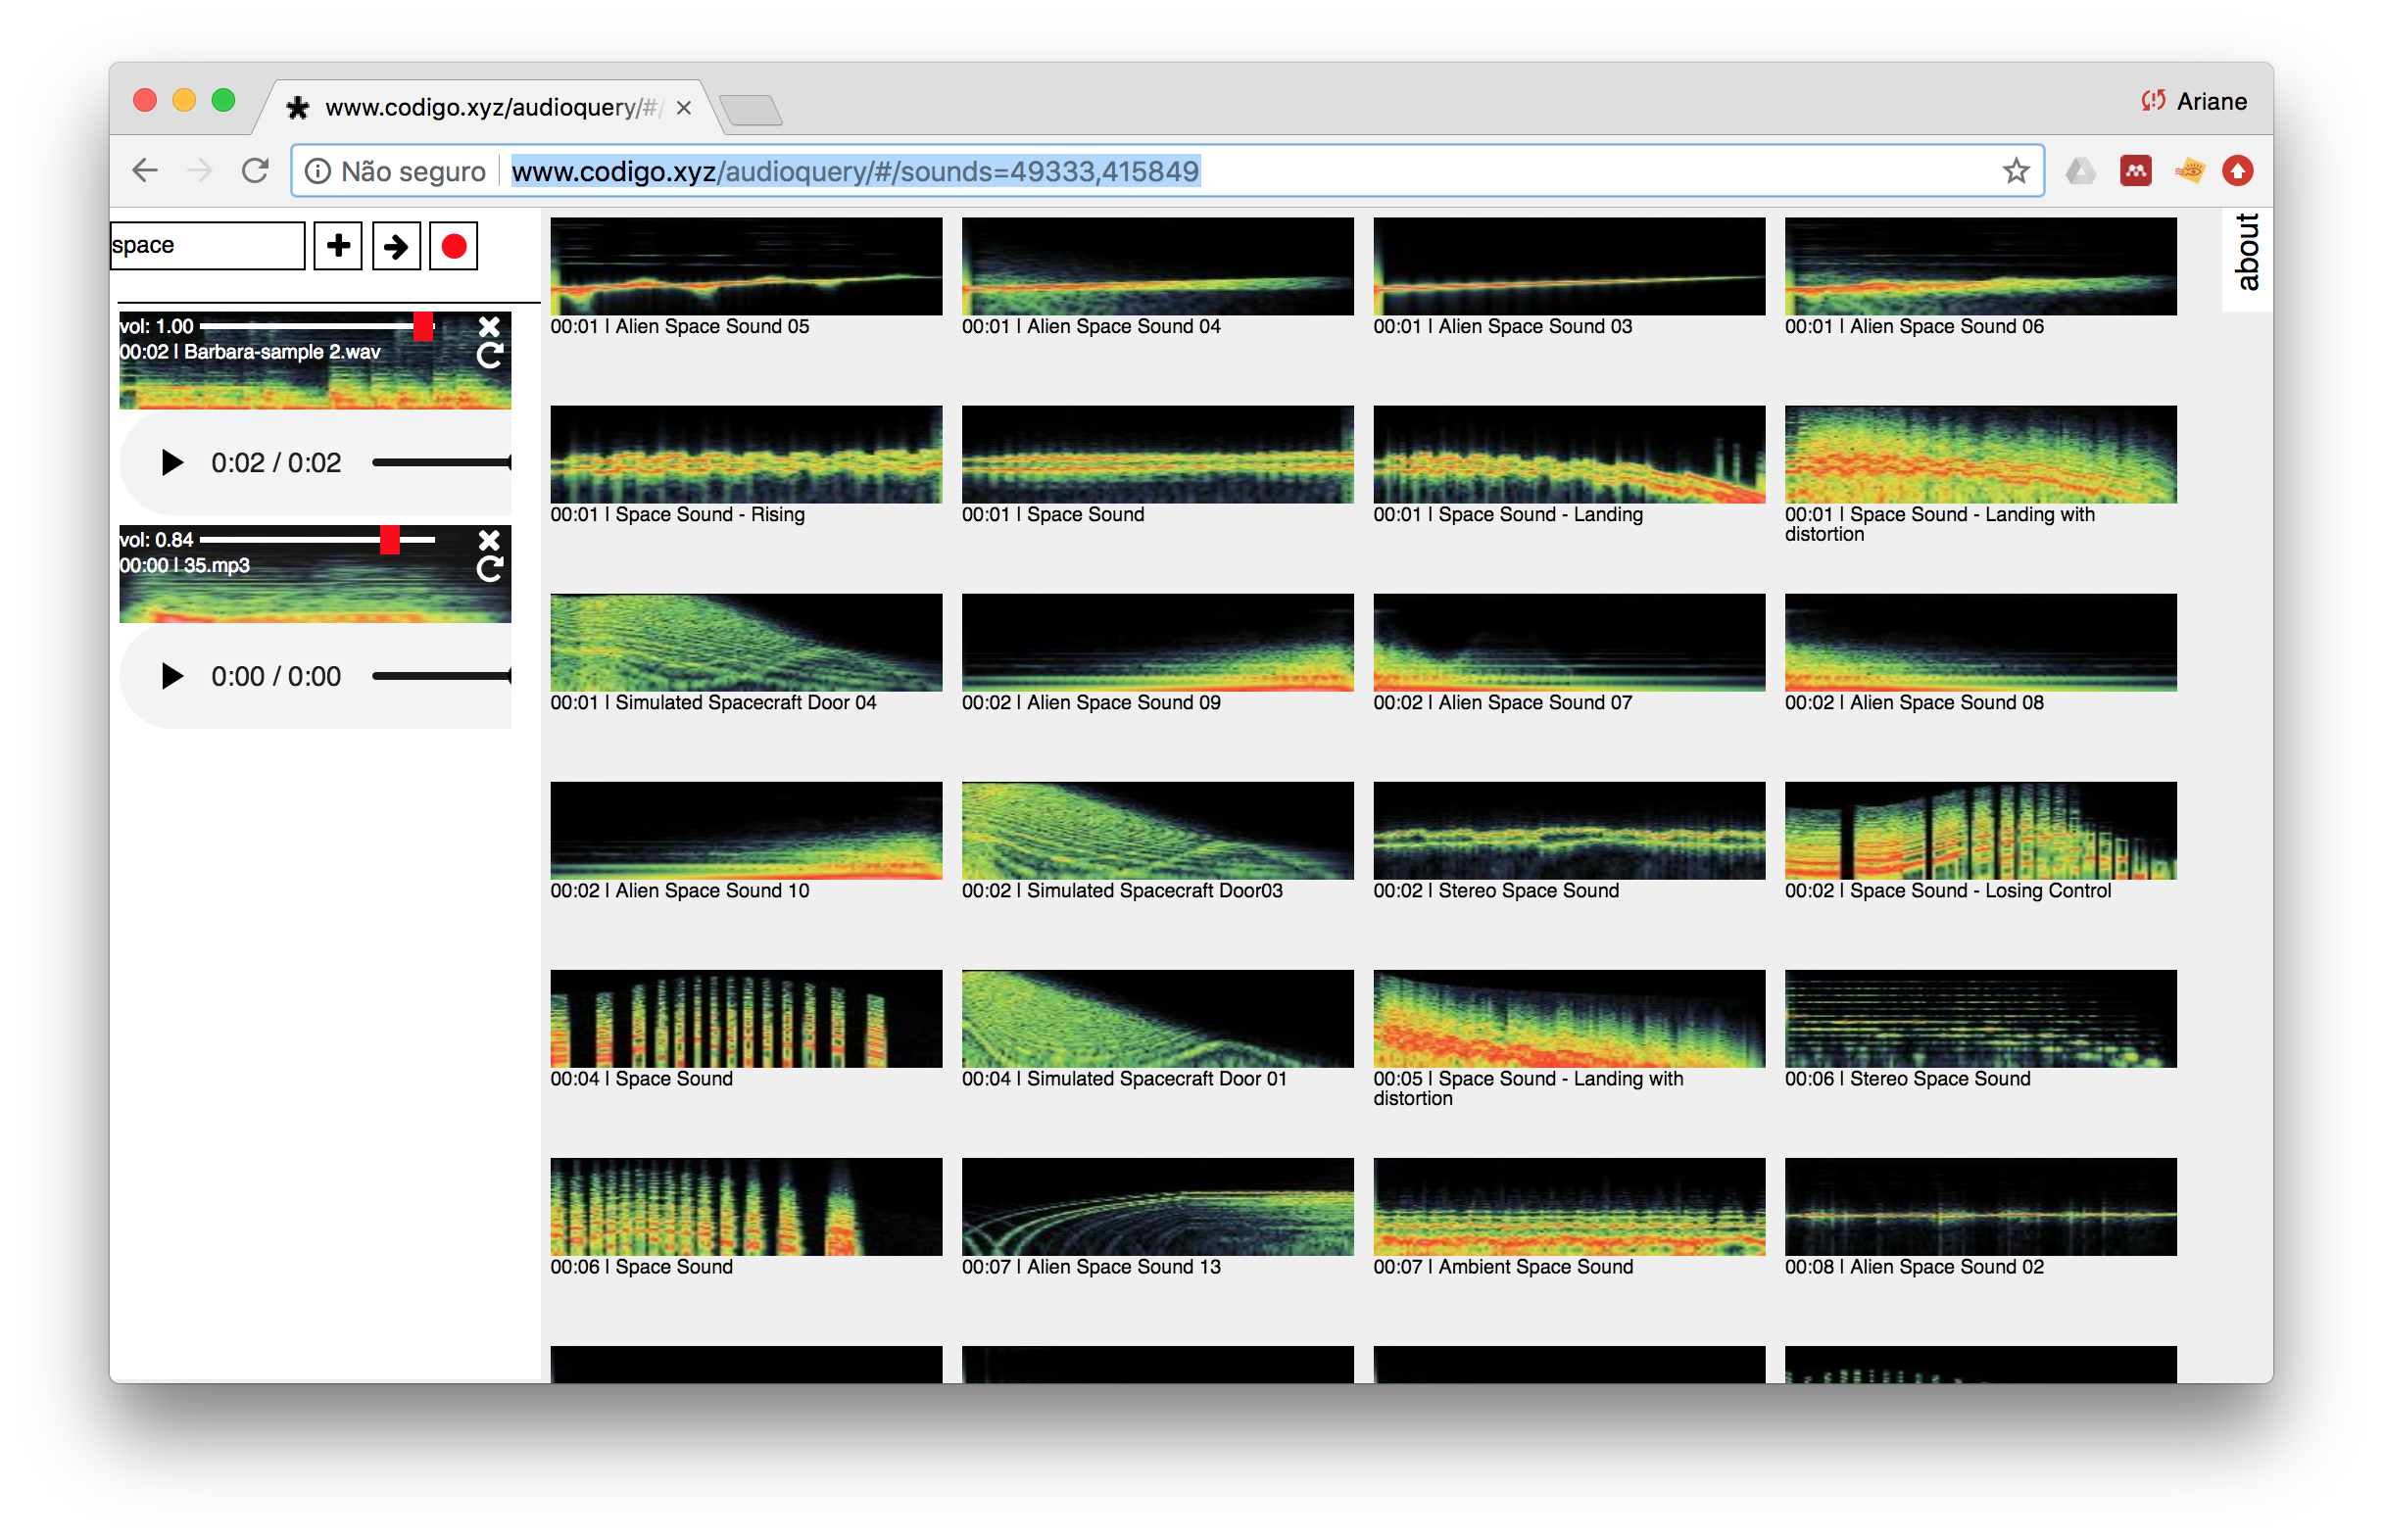
\includegraphics[width=0.8\textwidth]{pictures/cap4/audioquery}
\caption{\label{pstimeline}Primeira versão funcional do software desenvolvida.}
\label{fig:audioquery}
\end{figure}

 %Mais adiante, passei a contar com a ajuda da {}programadora Alessia Millo, que colaborou no desenvolvimento do tocador e de outros recursos que implantamos no sistema. Ela trabalhou na adaptação do sistema para utilizar as tecnologias de Web Audio, ao invés dos objetos HTML, que permitiu uma série de recursos que implementamos posteriormente, como a possibilidade de escolher o começo e o fim dos pontos de loop, alterar a velocidade de reprodução de sons e posição estéreo dos sons.




\end{otherlanguage*}

\phantomsection



    % Finaliza a parte no bookmark do PDF
    % para que se inicie o bookmark na raiz
    % e adiciona espaço de parte no Sumário
    \phantompart

    % Conclusão (outro exemplo de capítulo sem numeração e presente no sumário)
    % The \phantomsection command is needed to create a link to a place in the document that is not a
% figure, equation, table, section, subsection, chapter, etc.
%
% When do I need to invoke \phantomsection?
% https://tex.stackexchange.com/questions/44088/when-do-i-need-to-invoke-phantomsection
\phantomsection

% ---
% Considerações Finais (outro exemplo de capítulo sem numeração e presente no sumário)
% ---
\chapter*[]{\lang{Final Remarks}{Considerações Finais}}
\phantomsection
\addcontentsline{toc}{chapter}{Considerações Finais}%



\section{Porque fazer?}
\begin{citacao}
De volta à metade dos anos 1960, o mcluhanismo fora inventado
como o credo do Centro Vital. Duas décadas depois, o signifi cado dessa teoria essencial no meio da elite dos Estados Unidos moveu-se para a direita. Com a Esquerda da Guerra Fria desacreditada, muitos de seus membros acharam consolo ideológico no renascimento do liberalismo de livre mercado nos anos 1970: o neoliberalismo.\cite[347]{Barbrook2009}
\end{citacao}

\begin{citacao}
Dos sistemas de câmeras de vigilância aos programas de monitoramento de mensagens eletrônicas, o governo dos Estados Unidos e seus aliados sistematicamente adquiriam as ferramentas para uma vigilância constante de toda a população global. No setor privado, as tecnologias da informação similarmente revitalizaram as hierarquias tayloristas. (...) graças ao panóptico em rede, a elite corporativa era agora capaz de controlar suas vidas muito mais detalhadamente do que no passado fordista. O tecno-coletivismo do mcluhanismo metamorfoseou-se no tecno- autoritarismo da consultoria gerencial de McKinsey. \cite[345]{Barbrook2009}
\end{citacao}

``No momento em que todos tivessem acesso à Internet, a democracia participativa e a criatividade cooperativa seriam a ordem do dia. Entretanto'' \cite[360]{Barbrook2009}

\begin{citacao}
Todos os sonhos de democracia participativa e criatividade cooperativa seriam realizados dentro da aldeia global por vir. Em estágios iniciais da modernidade, esses princípios libertários foram somente parcialmente realizados. Felizmente, uma vez que estivessem conectados à Internet, todos – inclusive os descendentes dos escravos – desfrutariam dos benefícios da democracia da alta tecnologia jeffersoniana.
\end{citacao}
  
 \begin{citacao}
 
   A partir das relações do homem com a realidade, resultantes de estar com ela e de estar nela, pelos atos de criação, recriação e decisão, vai ele dinamizando o seu mundo. Vai dominando a realidade. Vai humanizando-a. Vai acrescentando a ela algo de que ele mesmo é o fazedor. Vai temporalizando os espaços geográficos. Faz Cultura. E é ainda o jogo destas relações do homem com o mundo e do mundo e do homem com os homens, desafiado e respondendo ao desafio, alterando, criando, que não permite a imobilidade, a não ser em termos de relativa preponderância, nem das sociedades nem das culturas. E, à medida que cria, recia e decide, vão se conformando as épocas históricas. É também criando, recriando e decidindo o que o homem deve participar destas épocas. \cite[60]{Freire2015}
    \end{citacao} 

   \begin{citacao}
   Uma das grandes, senão a maior, tragédia do homem moderno está em que é hoje dominado pela força dos mitos e comandado pela publicidade organizada, ideológica ou não, e por isso vem renunciando cada vez, sem o saber, à sua capacidade de decidir. Vem sendo expluso da órbita das decisões. As tarefas do seu tempo não são capatadas pelo homem simples, mas a eles apresentadas por uma ``elite" que as interpreta e as entrega em forma de receita, de prescrição a ser seguida. E, quando julga que se salva seguindo as prescrições, afoga-se no anonimato nivelador da massificação, sem esperança e sem fé, domesticado e acomodado: já não é sujeito. Rebaixa-se a puro objeto. Coisifica-se. \cite[60]{Freire2015}
 \end{citacao} 

As eleições de 2018 provaram o potencial destruidor dos novos meios de comunicação, esse sujeito objeto massificado, impulsionado pela era da pós-verdade, em ambientes completamente controlados por algoritmos que não se sabe o que e quem controlam. O projeto Banda Aberta foi uma tentativa de dialogar com isso, propor novas formas de interação, mas a relação de controle imposta pela separação condutor/audiência, compositor intérprete não me deixou ainda confortável. 

\begin{citacao}
A música não pode ser uma linguagem nem fixada, nem meramente codificada pelo uso. A música faz-se e inventa-se constantemente, procura-se um sentido, e qualquer passagem misteriosa e singular — na verdade bastante singular — entre natureza e
cultura. \cite{Schaeffer2007}

Decidir seguir a carreira de professora, de ter um compromisso com a educação e as potências que emanar dessas relações, faz pensar em ferramentas que possam ser apreendidas de uma maneira mais abrangente. Tive felizmente, no final deste processo a oportunidade de lecionar e utilizar minhas própias ferramentas em aula.


\footnote{\url{http://www.playsound.space/sounds=308270,308618,309333,290401,43461,314864,399466,295858,278084,334534,428800,246658,357370,355118,356661,374567,220747}}









\subsection{O que fazer?} 

\todo[inline]{posicionar essa citacao}
\begin{citacao}
Tanto multimídia como intermídia, são categorias interdisciplinares que, como colagem ou síntese-qualitativa, colocam em questão as formas de produção-criação individual e sobretudo a noção de autor. A criação é hoje o resultado da interação dessas práticas, como forma de tradução e inter-relação. O que não quer dizer que já não seja possível instaurar um estilo: ele é hoje a marca invariante que estabelece a diferença transmutadora em quaisquer dos suportes utilizados. O diálogo entre o singular-individual (ego) e o coletivo (superego) é uma das caracterísiticas da prática tecnológica. Por outro lado, os meios tecnológicos absorvem e incorporam os mais diferentes sistemas sígnicos, traduzindo as diferentes linguagens históricas para o novo suporte. Essas linguagens transcodificadas efetivam a colaboração entre os diversos sentidos, possibilitando o trânsito intersemiótico e criativo entre o visual, o verbal, o acústico e o tátil \cite[66]{JulioPlaza1969}
\end{citacao}

Os projetos desenvolvidos no decorrer desta tese também apontam para uma série de desejos de desenvolvimentos futuros. 

- ferramenta colaborativa
- tracker
- sons autorais
- remixagem com faixas 
- sintetizador
- radio
- upload

Playsound não é um produto, 




\end{citacao}





    % ELEMENTOS PÓS-TEXTUAIS
    \postextual
    \setlength\beforechapskip{0pt}
    \setlength\midchapskip{15pt}
    \setlength\afterchapskip{15pt}

    % Referências bibliográficas
    \begingroup
        % Using BibTeX to make a list of references without having citations in the body of the document?
        % https://tex.stackexchange.com/questions/17128/using-bibtex-to-make-a-list-of-references-without
        % \nocite{*}

        % How to modify line spacing per entry of bibliography?
        % https://tex.stackexchange.com/questions/163559/how-to-modify-line-spacing-per-entry-of-bibliography
        \linespread{1.18}\selectfont
        \printbibliography
\endgroup

    % Glossário, consulte o manual da classe abntex2 para orientações sobre o glossário.
    % \ifforcedinclude\else\glossary\fi

    % Apêndices, inicia os apêndices
    \begin{apendicesenv}
        % Imprime uma página indicando o início dos apêndices
        \ifforcedinclude\else\partapendices\fi

        \setlength\beforechapskip{50pt}
        \setlength\midchapskip{20pt}
        \setlength\afterchapskip{20pt}

        %
% How to fix the Underfull \vbox badness has occurred while \output is active on my memoir chapter style?
% https://tex.stackexchange.com/questions/387881/how-to-fix-the-underfull-vbox-badness-has-occurred-while-output-is-active-on-m
%

% ---

\lang
{\chapter[Appendix A]{Resources}}
{\chapter[Apêndice A]{Recursos}}
% ---


% Multiple-language document - babel - selectlanguage vs begin/end{otherlanguage}
% https://tex.stackexchange.com/questions/36526/multiple-language-document-babel-selectlanguage-vs-begin-endotherlanguage

 



% As this page is not being completely filled, it is generating the page bottom bad box.
% Fix Underfull \vbox (badness 10000) has occurred while \output is active
%
% \flushbottom vs \raggedbottom
% https://tex.stackexchange.com/questions/65355/flushbottom-vs-raggedbottom
\newpage

\section{Linguagens}
\subsection{HTML5}


\subsection{JavaScript}
\subsubsection{Node.js}
\subsubsection{Angular}
\subsubsection{JSON}



\subsection{CSS}

\subsection{API's}
\begin{citacao}
Massive amounts of digital data can now be researched, collected, interpreted, reformatted, and displayed for the purpose of art-making. This gives data a chance to be reborn toward aesthetic, communicative, or social purposes. Perhaps the simplest idea of this new art is the idea of copy and paste, allowing digitalized data to move from one location to another. From this core idea the rise of an internet culture, and network capabilities expands this to global dissemination of content. From here, the dynamics of this network culture permits artifacts to become art systems. All these aspects are dependent on the technological capacities. The technologies support these three aspects: cut/paste, networking and dissemination, and artifact/systems while simultaneously advancing the ease by which they can be performed. In this manner the collaboration is growing in both the number of participants as users and the number of participants as creators. Still, due to human practice and change through learning, our relationship to technology is always in fiery negotiation. The public Interface can be regarded as a technological construct as well as a cultural artifact as the elements in cyberspace (such as the dialogue and logic/ language patterns) become revealed via the interface. The art-making public interface is both the media and the message composited, it allows for sharing and repurposing. In this respect it fosters its own cultural artifact—artmaking that can be examined in its own right. The importance of this collective must be acknowledged as a heretofore unknown thing; this public interface has lead to a new art system. This is the foundation of a network aesthetic that will continue to evolve.
\cite[5]{Soon2011}
\end{citacao}

\subsubsection{WebAudio API}

\subsubsection{Freesound API}

\section{Ferramentas}
\subsection{Terminal}

\begin{citacao}
Linha de comando eh o maior maior barato
Você nunca mais vai esquecer
Dar um cat no arquivo
Ls pra listar
E pra mudar o diretório eh o cd (Articuladores, )
\end{citacao}

Operar através de linha de comando, é um dos primeiros aprendizados do hacker. Se estéticamente parece uma coisa obscura, misteriosa para usuário superficial de computadores, é uma tecnologia importante para vários processos de desenvolvimento de software, incluindo também para o controle de servidores, e gerenciamento de repositórios de código. A linha de comando, que é como se chama a interface para controle dos sistemas operacionais via texto remove a interface gráfica do usuário (GUI), que contém todas as metáforas de usabilidade desenvolvidas para tornar a computação um processo mais familiar para os usuário de uma maneira geral.

Ao remover essa camada, a linha de comando exige que o operador saiba os comandos para executar as tarefas necessárias ao seu trabalho, ou pelo menos saiba como procurar como saber, mas também permite um acesso mais direto e não mediado a estruturas de dados, aplicativos e ferramentas diversas. Compreender como funciona a linha de comando é em um certo sentido também libertador, ao passo que pode conferir agilidade e poder sobre meios digitais. 

Neste trabalho, a linha de comando serviu também como inspiração para a interface de controle do projeto Banda Aberta. Nele, os comandos para se trocar som, aumentar ou diminuir o volume funcionavam através de códigos que eram colados na conversação, que apenas algumas pessoas na audiência dominavam. 


\subsection{Git}
Git é uma ferramenta de controlde de versões voltadas para se criar repositórios de códigos fonte. Além do Git existem outras ferramentas similares, como CVN Com o Git, é possível que uma equipe compartilhe os mesmos arquivos, que ficam organizados em um servidor central. O git tem uma interface gráfica, mas é mais prático e eficiente de ser usado através da linha de comando. 

Quando se criamos um repositório, podemos incluir arquivos que podem ser copiados por qualquer pessoa que tiver acesso a ele. Existem repositórios provados, aos quais você em geral precisa ter que pagar, mas se você estiver disposto a disponibilizar seu código como software livre, exitem vários serviços gratuitos para hospedagem online, como Github, Bitbucket etc. 

O sistema permite que se criem galhos ou \emph{branches}, que são versões em paralelo do software em questão, e também guarda todas alterações enviadas pelos colaboradores do projeto. Funciona como sistema de backup, mas é importante principalmente para o desenvolvimento de projetos colaborativos que envolvem mais de um programador. 

Neste projeto, utilizamos o Github como plataforma para disponibilização de todos os códigos fonte desenvolvidos durante o projeto, como os do Banda Aberta, Spectrogram Player e Playsound, e também os próprios códigos fonte desta tese, que foi escrita em LaTex.

\subsection{LaTex}

Latex é uma linguagem de programação voltada para a escrita de textos científicos. Ao escrever em LaTex, a parte burocrática da escrita científica, como numerar figuras, tabelas e notas de rodapé, gerar bibliografias e posicionar figuras é feita automaticamente pelo sistema. A aparência gráfica da página é definida por um modelo, ou \emph{template}, que pode ser copiado ou fornecido por uma instituição ou comitê científico por exemplo.

A descoberta do Latex como ferramenta de produção foi de extrema importância no desenvolvimento deste projeto de pesquisa, e facilitou a produção de nove artigos que foram publicados durante esse processo. Para isso, fiz uso também da ferramenta online Overleaf, que fornece acesso online a uma ferramenta de edição colaborativa e visualização de arquivos LaTex. Para o desenvolvimento desta tese, no entanto, em um determinado momento foi necessária a migração para um ambiente de desenvolvimento local pela quantidade de arquivos que não era suportada pela versão gratuita do sistema. Além disso, com o ambiente de desenvolvimento local foi possível se desvenciliar da necessidade de conecção de internet para a escrita do documento.

\subsection{}




\subsubsection{ }





    \end{apendicesenv}

    % Anexos, inicia os anexos
    \begin{anexosenv}
        % Imprime uma página indicando o início dos anexos
        \ifforcedinclude\else\partanexos\fi

        \setlength\beforechapskip{50pt}
        \setlength\midchapskip{20pt}
        \setlength\afterchapskip{20pt}

        %
% How to fix the Underfull \vbox badness has occurred while \output is active on my memoir chapter style?
% https://tex.stackexchange.com/questions/387881/how-to-fix-the-underfull-vbox-badness-has-occurred-while-output-is-active-on-m
%

% ----------------------------------------------------------
\chapter{\lang{Article published in SOBRAEP magazine}{Artigo publicado}}
% ----------------------------------------------------------


% Multiple-language document - babel - selectlanguage vs begin/end{otherlanguage}
% https://tex.stackexchange.com/questions/36526/multiple-language-document-babel-selectlanguage-vs-begin-endotherlanguage
\begin{otherlanguage*}{english}

% An environment for setting \emergencystretch locally
% https://tex.stackexchange.com/questions/84510/an-environment-for-setting-emergencystretch-locally
{
    \setlength{\emergencystretch}{10pt}
    \section[English guidelines for publication]
    {English guidelines for publication - TITLE HERE (14 PT TYPE SIZE, UPPERCASE, BOLD, CENTERED)}
}
    \noindent\textbf{Abstract:}
    The objective of this document is to instruct the authors about the preparation of the
    manuscript for its submission to the Revista Eletrônica de Potência (Brazilian Power Electronics
    Journal).~The authors should use these guidelines for preparing both the initial and final
    versions of their paper. Additional information about procedures and guidelines for publication
    can be obtained directly with the editor, or through the web site
    \url{http://www.sobraep.org.br/revista}. This text was written according to these guidelines

\end{otherlanguage*}

% What is a “Overfull \hbox (9.89561pt too wide)”?
% https://tex.stackexchange.com/questions/111948/what-is-a-overfull-hbox-9-89561pt-too-wide
interwordspace: \the\fontdimen2\font

interwordstretch: \the\fontdimen3\font

emergencystretch: \the\emergencystretch\par\relax


%|||||||||||||||||||||||||||||||||
%para incluir outro pdf descomentar abaixo

%\modifiedincludepdf{-}{ArtigoSOBRAEP}{pictures/SOBRAEP.pdf}{0.9}



        %
% How to fix the Underfull \vbox badness has occurred while \output is active on my memoir chapter style?
% https://tex.stackexchange.com/questions/387881/how-to-fix-the-underfull-vbox-badness-has-occurred-while-output-is-active-on-m
%

% ----------------------------------------------------------
\lang
{\chapter[Sample example]{How to display the font size in use in the final output}}
{\chapter[Anexo exemplo]{Como exibir o tamanho da fonte em uso na saída final}}
% ----------------------------------------------------------


% Multiple-language document - babel - selectlanguage vs begin/end{otherlanguage}
% https://tex.stackexchange.com/questions/36526/multiple-language-document-babel-selectlanguage-vs-begin-endotherlanguage
\begin{otherlanguage*}{english}

 

1. How to display the font size in use in the final output,
2. How to display the font size in use in the final output,
3. How to display the font size in use in the final output,


\section[Some encoding tests]{ }

1. How to display the font size in use in the final output,
2. How to display the font size in use in the final output,
3. How to display the font size in use in the final output,
4. How to display the font size in use in the final output,
5. How to display the font size in use in the final output,
6. How to display the font size in use in the final output,

7. How to display the font size in use in the final output,
8. How to display the font size in use in the final output,
9. How to display the font size in use in the final output,
10. How to display the font size in use in the final output,
11. How to display the font size in use in the final output,
12. How to display the font size in use in the final output,

\subsection{ }

1. How to display the font size in use in the final output,
2. How to display the font size in use in the final output,
3. How to display the font size in use in the final output,
4. How to display the font size in use in the final output,
5. How to display the font size in use in the final output,
6. How to display the font size in use in the final output,

7. How to display the font size in use in the final output,
8. How to display the font size in use in the final output,
9. How to display the font size in use in the final output,
10. How to display the font size in use in the final output,
11. How to display the font size in use in the final output,
12. How to display the font size in use in the final output,

\subsubsection{ }

1. How to display the font size in use in the final output,
2. How to display the font size in use in the final output,
3. How to display the font size in use in the final output,
4. How to display the font size in use in the final output,
5. How to display the font size in use in the final output,
6. How to display the font size in use in the final output,

7. How to display the font size in use in the final output,
8. How to display the font size in use in the final output,
9. How to display the font size in use in the final output,
10. How to display the font size in use in the final output,
11. How to display the font size in use in the final output,
12. How to display the font size in use in the final output,

\subsubsubsection{ }

1. How to display the font size in use in the final output,
2. How to display the font size in use in the final output,
3. How to display the font size in use in the final output,
4. How to display the font size in use in the final output,
5. How to display the font size in use in the final output,
6. How to display the font size in use in the final output,
7. How to display the font size in use in the final output,

8. How to display the font size in use in the final output,
9. How to display the font size in use in the final output,
10. How to display the font size in use in the final output,
11. How to display the font size in use in the final output,
12. How to display the font size in use in the final output,


Lipsum me [55-65]

\end{otherlanguage*}



    \end{anexosenv}

    % INDICE REMISSIVO
    \ifforcedinclude\else
        \phantompart
        \printindex
    \fi

\end{document}

